\documentclass[12pt,a4paper,twoside,openright]{book}
% the book class has some advantages over the report class
% it defines three styles: frontmatter, mainmatter and backmatter
% the default styles are very convenient
% Load packages
% !TeX root=../main_file.tex
% !TeX TS-program = pdflatex
% !TeX checkspelling = fr-toutesvariantes


%--------------------------------------------------------
%				LANGUAGE SETTINGS
%--------------------------------------------------------
\usepackage[french]{babel}


%--------------------------------------------------------
%				PAGE DIMENSIONS
%--------------------------------------------------------
\usepackage[left=2.5cm, right=2.5cm, top=2cm, bottom=2cm]{geometry}
\usepackage{changepage}

%--------------------------------------------------------
%					GRAPHICS
%--------------------------------------------------------
% Packages for pictures adding
\usepackage{float}
\usepackage{graphicx} %insert images
\usepackage{caption}
\usepackage{subcaption}

\graphicspath{{../../../../1-Bibliography/Pictures/}%
				{./src/mainmatter/chapter_1/figures/}
				{./src/mainmatter/chapter_2/figures/}
				{./src/mainmatter/chapter_3/figures/}
				{./src/mainmatter/chapter_4/figures/}
				{./src/mainmatter/chapter_5/figures/}
}


%--------------------------------------------------------
%					REFERENCES 
%--------------------------------------------------------
%\usepackage[sectionbib]{chapterbib} % add references, sectionbib option adds the references in each chapter
%\usepackage[numbers,square]{natbib}
\usepackage[backend=biber,
bibstyle=ieee, 
citestyle=numeric-comp,
natbib=true,
doi=false, 
url=false,
isbn=false,
mincitenames=1,
maxcitenames=1,
minbibnames=1,
maxbibnames=99,
backref=false,]
{biblatex}
\addbibresource[label=main_bib]{./src/backmatter/PhD.bib}


%--------------------------------------------------------
%				FONT SETTINGS
%--------------------------------------------------------
\usepackage{ifxetex}
% XELATEX SPECIFICATIONS
\ifxetex
	\usepackage{unicode-math}
	\usepackage{fontspec} % Font selection for XeLaTeX; see fontspec.pdf for documentation
	\defaultfontfeatures{Mapping=tex-text} % to support TeX conventions like ``---''
	\usepackage{xunicode} % Unicode support for LaTeX character names 
	\usepackage{unicode-math}
	\usepackage{xltxtra} % Extra customizations for XeLaTeX
	\setmainfont{CMU Concrete} %if the font is installed on the system
	\setmathfont{CMU Concrete}
	\setsansfont{CMU Sans Serif}
	\setmonofont{CMU Typewriter Text}
\else
% PDFLATEX SPECIFICATIONS
	\usepackage{microtype}% better space management
	\usepackage[utf8]{inputenc}%utf encoding
	\usepackage[T1]{fontenc}
	%\usepackage{default} %load the default police pack
	%\usepackage[amsfonts,amssymb,exscale]{concmath}
	\usepackage{mathastext}
	%\renewcommand*\familydefault{\ttdefault}
	%available packs: default, bookman, charter, newcent, lmodern, mathpazo, mathptmx
	
\fi

%--------------------------------------------------------
%		HEADERS AND FOOTERS 
%--------------------------------------------------------

%Custom headers and footers
\usepackage{fancyhdr} %custom headers and footers layout
\usepackage{lastpage} %package to print the last page
\pagestyle{fancy} %fancy page style
\fancyhf{}
\fancyhead[LE, LO]{\leftmark}
\fancyfoot[CO,CE]{\thepage}
%redefine headers for 
%No capitalization
\renewcommand{\sectionmark}[1]{%
\markright{
\ \thesection.\ #1}{}}

\renewcommand{\chaptermark}[1]{%
\markboth{\chaptername
\ \thechapter.\ #1}{}}


%--------------------------------------------------------
%				MATHS TOOLS
%--------------------------------------------------------
% amsmath and amsfont have to be loaded before the xunicode package when XeTeX is used. 
% The experimental package unicode-math will subsitute those packages when XeTeX is used. 
% It is available in TeX Live 2012.
\usepackage{amsmath}
\usepackage{amsfonts} 
\usepackage{amssymb}
\usepackage{amsthm}
% The amsthm package provides an enhanced version of LATEX's \newtheorem commandfor defining theorem-like environments.
\usepackage{mathtools} 
% The mathtools package fixes some amsmath quirks and adds some useful settings, symbols, and environments to amsmath. The mathtools package loads the amsmath package and hence there is no need to 

%--------------------------------------------------------
%			ADDITIONAL PACKAGES 
%--------------------------------------------------------
% diverse package
\usepackage{textcomp} %use specific symbols for text (example "°")
\usepackage{multicol} %create multi column environment

% use colors
\usepackage{color}
\usepackage[table]{xcolor}
\usepackage{array}
\usepackage{multirow}

\usepackage{booktabs}% add top, middle, bottom rule for professional tables

\usepackage{siunitx} %Use SI units
%\usepackage[Lenny]{fncychap}% change the chapter aspect
% Lenny, Sonny, Glenn, Conny, Rejne, Bjarne, Bjornstrup
%\ChTitleVar{\mdseries \sc}


\usepackage{varioref}% change the reference style of the floats
\usepackage{setspace}% interspacing management

%\usepackage{sectsty}
%\allsectionsfont{\mdseries \sc}
\usepackage{minitoc}% add TOC in each chapter
\mtcselectlanguage{french} % change language in minitoc package
\mtcsetdepth{minitoc}{1}
% \usepackage{listings} %add programmation code p.199 in latex tutorial

% ToC (table of contents) APPEARANCE
%\usepackage[nottoc,notlof,notlot]{tocbibind} % Put the bibliography in the ToC
%\usepackage[titles,subfigure]{tocloft} % Alter the style of the Table of Contents
%\renewcommand{\cftchapfont}{\mdseries \sc}
%\renewcommand{\cftchappagefont}{\mdseries} % No bold!
%\renewcommand{\cftsecfont}{\mdseries \sc}
%\renewcommand{\cftsecpagefont}{\mdseries} % No bold!
\usepackage{lipsum}
%--------------------------------------------------------
%			INDEX AND NOMENCLATURE 
%--------------------------------------------------------
\usepackage[french]{nomencl}
\renewcommand{\nomgroup}[1]{%
\ifthenelse{\equal{#1}{A}}{\item[\textbf{Sigles}]}{%
\ifthenelse{\equal{#1}{I}}{\item[\textbf{Indices}]}{%
\ifthenelse{\equal{#1}{C}}{\item[\textbf{Constantes Physiques}]}{%
\ifthenelse{\equal{#1}{E}}{\item[\textbf{Electrochimie}]}{%
\ifthenelse{\equal{#1}{P}}{\item[\textbf{Photoélectrochimie}]}%
{}
}% matches Subscripts
}% matches Abbreviations
}
}
}

\makenomenclature
\usepackage{makeidx}
\makeindex


%--------------------------------------------------------
%			PDF PROPERTIES AND HYPERLINKS 
%--------------------------------------------------------

% url links in document
\usepackage{url}
\usepackage{hyperref}
\usepackage{csquotes}




%--------------------------------------------------------
%			CUSTOM ENVIRONMENTS 
%--------------------------------------------------------
\newenvironment{abstract}%
{\null \vspace{\stretch{1}}\begin{center}%
\bfseries \large \abstractname \end{center}}%
{\vspace{\stretch{4}}\null}

\makeatletter
\newenvironment{chapintroduction}{%
    \vspace{1cm} \begin{adjustwidth}{0.5cm}{0.5cm}\it }%
   {\end{adjustwidth}\par}
\makeatother

\newenvironment{acknowledgement}%
{\cleardoublepage\null \vspace{\stretch{1}}\begin{center}%
\bfseries Remerciements \end{center}}%
{\vspace{\stretch{2}}\null}

\newenvironment{dedication}%
{\clearpage\begin{flushright} \null\vspace{\stretch{1}}}%
{\vspace{\stretch{2}}\null \end{flushright}}


%--------------------------------------------------------
%	CUSTOM COLORS
%--------------------------------------------------------
\definecolor{lightgray}{gray}{0.9}

\setcounter{secnumdepth}{4}
\setcounter{tocdepth}{2}

\DeclareSIUnit\ppm{ppm}
\DeclareSIUnit\ppb{ppb}
\DeclareSIUnit\dec{dec}
\newcommand{\Hyd}{$\rm H_2$}
\newcommand{\Oxy}{$\rm O_2$}
\newcommand{\Tkim}{\SI{300}{\degreeCelsius}}
\newcommand{\E}{E}
\newcommand{\SC}{sc}
\newcommand{\cc}{cc}
\newcommand{\iph}{I_{ph}}
\newcommand{\ipht}{I_{ph}^{\ast}}
\newcommand{\phase}{\theta}
\newcommand{\Hm}{H}
\newcommand{\el}{el}
\newcommand{\DRe}{D^2_{Re}}
\newcommand{\DIm}{D^2_{Im}}
\newcommand{\ReIphtExp}{Re \, I_{ph,exp}^{\ast}}
\newcommand{\ReIphtCalc}{Re \, I_{ph,calc}^{\ast}}
\newcommand{\ImIphtExp}{Im \, I_{ph,exp}^{\ast}}
\newcommand{\ImIphtCalc}{Im \, I_{ph,calc}^{\ast}}
\newcommand{\ReIphExp}{Re \, I_{ph,exp}}
\newcommand{\ReIphCalc}{Re \, I_{ph,calc}}
\newcommand{\ImIphExp}{Im \, I_{ph,exp}}
\newcommand{\ImIphCalc}{Im \, I_{ph,calc}}

\newcommand{\hv}{h\nu}

\renewcommand{\theparagraph}{\alph{paragraph})}


% INPG TITLE PAGE
\usepackage[a4paper]{./src/meta-donnees}

% PDF properties displayed as metadata
\hypersetup{
    bookmarks=true, 		% show bookmarks bar?
    unicode=true,  		% non-Latin characters in Acrobat’s bookmarks
    pdftoolbar=true,        % show Acrobat’s toolbar?
    pdfmenubar=true,        % show Acrobat’s menu?
    pdffitwindow=true,      % page fit to window when opened
    pdftitle={Etude (photo)-électrochimique en réacteur simulé du phénomène de shadow corrosion des alliages de zirconium},    % title
    pdfauthor={M. Skocic},     % author
    pdfsubject={PhD},   % subject of the document
    pdfnewwindow=true,      % links in new window
    pdfkeywords={Shadow Corrosion, PEC, Electrochimie, In-Situ}, % list of keywords
    colorlinks=False,       % false: boxed links; true: colored links
    linkcolor=red,          % color of internal links
    citecolor=green,        % color of links to bibliography
    filecolor=magenta,      % color of file links
    urlcolor=cyan           % color of external links
}
%Work around for biblatex-ieee
%Proper capital protection in title
%\DeclareFieldFormat{titlecase}{\MakeCapital{#1}}
\DeclareFieldFormat{sentencecase}{\MakeSentenceCase{#1}}

\captionsetup[table]{name=\textsc{Tableau}}
% Avoid dash for same author in 2 consecutive citations (IEEE style)
\renewbibmacro*{bbx:savehash}{}
\usepackage{setspace}
\pdfminorversion=7
%\pdfobjcompresslevel=0
%\usepackage[a-1b]{pdfx}

%\setlength{\parindent}{0cm}

%--------------------------------------------------------
%				DOCUMENT
%--------------------------------------------------------
%\includeonly{./mainmatter/chapter_1/chapter_1}
\begin{document}

% french for the whole document
% english is activated at the end for the summary in english
%\selectlanguage{french}

%%%%%%%%%%%%%%%%%%%%%%%%%%%%%%%
%%%%%%%% FRONT MATTER %%%%%%%%%
%%%%%%%%%%%%%%%%%%%%%%%%%%%%%%%
	% Front matter starts here
	\frontmatter
	\pagestyle{plain} %avoid headers from fancyhdr package
	
	% Title page -INPG template
	% la ligne ci-dessous est à insérer obligatoirement dans le préambule du document avant \begin{document}

%\usepackage[a4paper]{meta-donnees}


% les lignes en bas sont à insérer obligatoirement après \begin{document}

%%%%%%%%%%%%%%%%%%%%%%%%%%%%%%%%%%%%%%%%%%%%%%%%%%%%%%
%%             Commandes Meta-données               %%
%%   à renseigner par les auteurs pour générer      %%
%%     la couverture modèle Univ. Grenoble          %%
%%%%%%%%%%%%%%%%%%%%%%%%%%%%%%%%%%%%%%%%%%%%%%%%%%%%%%
%%      Fichier encodé au format ISO-8859-16        %%

%\Sethpageshift{???mm}   %%optionnel : à décommenter si besoin pour ajout d'espace afin de center la couvérture horizontalement (valeur par défaut est -5.5mm)
%\Setvpageshift{???mm}   %%optionnel : à décommenter si besoin pour ajout d'espace afin de center la couvérture verticalement (valeur par défaut est -15.5mm)


%\Universite{}    %%optionnel : à décommenter et à renseigenr si vous voulez changer le non d'université
%\Grade{}         %%optionnel : à décommenter et à renseigenr si vous voulez changer le grade
\Specialite{Matériaux, Mécanique, Génie Civil, Electrochimie}
\Arrete{7 Août 2006}
\Auteur{Milan Skocic}
\Directeur{Jean-Pierre Petit}
\CoDirecteur{Yves Wouters}    %%optionnel : à décommenter et à renseigenr si présence d'un Co-directeur de thèse
\Laboratoire{Laboratoire SIMaP}
\EcoleDoctorale{l'Ecole Doctorale I-MEP2}         
\Titre{Etude (photo)-électrochimique en réacteur simulé du phénomène de shadow corrosion des alliages de zirconium}
%\Soustitre{}      %%optionnel : à décommenter et à renseigenr si présence d'un sous-titre de thèse
\Depot{27 mai 2016}       


% Commande pour création de nouvelles catégories dans le jury:

%\UGTNewJuryCategory{...NomDeLaCategorie...}{...Definition...}

% Exemple \UGTNewJuryCategory{UGTFamille}{Membre de la famille} que nous ajoutons dans la commande \Jury ci-dessous sous la forme \UGTFamille{Jean Rousseau}{(...titre_et_affiliation...s'il_y_en_a...)}


\Jury{
\UGTPresident{M., Marian CHATENET, }{Professeur, Université Grenoble Alpes}
%\UGTPresidente{Civilité, Prénom-et-Nom}{titre-et-affiliation}

\UGTRapporteur{M., Sébastien CHEVALIER}{Professeur, Université de Bourgogne}      %% 1er rapporteur
 
\UGTRapporteur{M., Marc TUPIN}{Ingénieur chercheur, CEA Saclay}     %% 1er examinateur
\UGTExaminateur{M., Damien KACZOROWSKI}{Ingénieur expert corrosion, Areva}     %% second examinateur

% Directeur de thèse
\UGTCoDirecteur{M., Yves WOUTERS}{Professeur, Université Grenoble Alpes}     

\UGTDirecteur{M., Jean-Pierre PETIT}{Professeur, Université Grenoble Alpes}{, Invité}
}

\MakeUGthesePDG    


	
	% Acknowledgment
	% !TEX root = ../main_file.tex

\begin{acknowledgement}
	
Je tiens à exprimer ma gratitude à mes encadrants académiques Jean-Pierre Petit et Yves
Wouters qui se sont montrés disponibles, efficaces et solidaires.
 
Je tiens également à remercier mon responsable industriel d'Areva, Damien Kaczorowski, pour la confiance qu'il m'a
accordé et son engagement dans la réalisation de ce travail de thèse. 

Je souhaite également remercier les membres de l'équipe SIR du laboratoire SIMaP ainsi
que les membres de l'équipe chimie de l'eau du Centre Technique d'Areva pour leur accueil et pour leur soutient.



\end{acknowledgement}

	
	%allows to add mini TOC for each chapter
	\dominitoc 
	
	%TOC + LOF + LOT
	\tableofcontents
	\listoffigures
	\listoftables
	% Nomenclature	
	% !TEX root = ../main_file.tex


% CONSTANTS
\nomenclature[C0102]{h}{Constante de Planck}
\nomenclature[C0103]{c}{Vitesse de la lumière dans le vide}
\nomenclature[C0105]{F}{Constante de Faraday}
\nomenclature[C0106]{R}{Constante universelle des gaz parfaits}
\nomenclature[C0107]{k}{Constante de Boltzmann}
\nomenclature[C0108]{e}{Charge élémentaire}
\nomenclature[C0108]{$\epsilon _0$}{Permittivité du vide}



% ELECTROCHEMISTRY

\nomenclature[E0099]{$\alpha _a$}{Coefficient de transfert anodique}
\nomenclature[E0100]{$\alpha _c$}{Coefficient de transfert cathodique}
\nomenclature[E0101]{$b_a$}{Pente de Tafel pour la branche anodique}
\nomenclature[E0102]{$b_c$}{Pente de Tafel pour la branche cathodique}
\nomenclature[E0103]{z}{Nombre d'électrons échangés}
\nomenclature[E0104]{$j$}{Densité de courant}
\nomenclature[E0105]{$j_0$}{Densité de courant d'échange}
\nomenclature[E0106]{U}{Potentiel électrochimique, mesuré ou appliqué, par rapport à une référence}
\nomenclature[E0107]{$U_{eq}$}{Potentiel électrochimique à l'équilibre mesuré par rapport à une référence}
\nomenclature[E0108]{$U_{fb}$}{Potentiel de bande plate par rapport à une référence}
\nomenclature[E0109]{$\eta$}{Surtension ($U-U_{eq}$)}


% PHOTOELECTROCHESMITRY
\nomenclature[P0101]{$\Phi _{\SC}$}{Potentiel électrique dans le semiconducteur}
\nomenclature[P0102]{$\Phi _{el}$}{Potentiel électrique dans l'électrolyte}
%\nomenclature[P0103]{$\Delta\Phi _{\SC/el}$}{Différence de potentiel entre le semiconducteur et l'électrolyte}
\nomenclature[P0105]{$\epsilon$}{Permittivité diélectrique relative}
\nomenclature[P0106]{$w_{sc}$}{Epaisseur de la charge d'espace}
\nomenclature[P0107]{$w_{\Hm}$}{Epaisseur de la double couche électrochimique}
\nomenclature[P0108]{$L_{\cc}$}{Longueur de diffusion moyenne des porteurs de charge minoritaires}

\nomenclature[P0201]{$\lambda$}{Longueur d'onde de la lumière}
\nomenclature[P0202]{$\nu$}{Fréquence de la lumière}
\nomenclature[P0203]{h$\nu$ ou E}{Energie de la lumière}
\nomenclature[P0204]{$\alpha _{\SC}$}{Coefficient d'absorption du semiconducteur}
\nomenclature[P0205]{$\phi$}{Flux de photon}

\nomenclature[P0301]{$\iph$}{Photocourant tel que mesuré (valeur complexe)}
\nomenclature[P0301]{$\ipht$}{Photocourant rapporté à un flux de photons normalisé (valeur complexe)}
\nomenclature[P0302]{$\theta$}{Phase entre le signal mesuré et le signal de référence correspondant au retard de
l'établissement du photocourant par rapport à l'illumination}
\nomenclature[P0303]{K}{facteur d'amplitude du photocourant correspondant à la pente de la transformée linéaire $(\vert
I_{ph}^{\ast} \cdot \vert h\nu)^{1/2}=f(h\nu - E_g)$ (loi de Gärtner-Butler)}


\nomenclature[P0400]{$\E_g$}{Largeur de bande interdite (gap)}
\nomenclature[P0401]{$\E_F$}{Niveau de Fermi}
\nomenclature[P0402]{$\E_c$}{Niveau d'énergie correspondant au bas de la bande de conduction}
\nomenclature[P0403]{$\E_{cs}$}{Niveau d'énergie correspondant au bas de la bande de conduction en surface}
\nomenclature[P0404]{$\E_v$}{Niveau d'énergie correspondant au haut de la bande de valence}
\nomenclature[P0405]{$\E_{vs}$}{Niveau d'énergie correspondant au haut de la bande de valence en surface}
\nomenclature[P0406]{$\E_d$}{Niveau d'énergie donneur dans le cas d'un dopage de type \emph{n}}
\nomenclature[P0407]{$\E_a$}{Niveau d'énergie accepteur dans le cas d'un dopage de type \emph{p}}
\nomenclature[P0408]{$\E_{fb}$}{Niveau de Fermi en situation de bandes plates}


% ABBREVIATIONS

\nomenclature[A0100]{BWR}{Boiling Water Reactor}
\nomenclature[A0102]{PWR}{Pressurized Water Reactor}
\nomenclature[A0103]{CRUD}{Chalk River Unidentified Deposits}
\nomenclature[A0104]{ESSC}{Enhanced Spacer Shadow Corrosion}
\nomenclature[A0105]{IAEA}{International Atomic Energy Agency}
\nomenclature[A0201]{PEC}{PhotoElectroChimie}
\nomenclature[A0202]{SHE}{Standard Hydrogen Electrode}
\nomenclature[A0203]{SCE}{Saturated Calomel Electrode}
\nomenclature[A0204]{MSE}{Mercury Sulphate Electrode}
\nomenclature[A0205]{OCV}{Open Circuit Voltage}
\nomenclature[A0206]{ZRA}{Zero Resistance Ammeter}
\nomenclature[A0301]{PEEK}{PolyEtherEtherKetone}
\nomenclature[A0302]{PTFE}{PolyTetraFluoroEthylene}
\nomenclature[A0401]{ppm}{Parts Per Million (rapport massique)}
\nomenclature[A0402]{ppb}{Parts Per Billion (rapport massique)}

\renewcommand{\nomname}{Liste des principaux sigles et notations utilisés dans le manuscrit}
\renewcommand{\nomlabel}[1]{#1\hfill}
\printnomenclature





%%%%%%%%%%%%%%%%%%%%%%%%%%%%%%%
%%%%%%% MAIN MATTER %%%%%%%%%%%
%%%%%%%%%%%%%%%%%%%%%%%%%%%%%%%
	
%  Avoid headers and footers when an empty page is added just before a new chapter. 
	\makeatletter
	\def\cleardoublepage{\clearpage\if@twoside
	\ifodd\c@page
	\else\hbox{}\thispagestyle{empty}\newpage
	\if@twocolumn\hbox{}\newpage\fi\fi\fi}
	\makeatother
	
	% The main matter starts here
	\mainmatter
    \raggedbottom
    \setlength{\parskip}{0.15cm}
    \onehalfspacing
	\pagestyle{plain}
	%Chapters
	% !TEX root = ../../main_file.tex
% !TeX TS-program = pdflatex
% !TeX checkspelling = fr-toutesvariantes

\chapter*{Introduction}\label{chap:introduction}
\phantomsection
\addstarredchapter{Introduction}
%\begin{refsection}

Dans les réacteurs nucléaires, la première barrière de confinement du combustible est assurée par la gaine en alliage 
de zirconium. La gaine représente donc un enjeu capital en termes de durabilité face à l'environnement agressif
d'un coeur de réacteur. Le vieillissement, et plus précisément l'oxydation des gaines, est un facteur de limitation de la durée de
vie des assemblages de combustible.

Ce travail de thèse, réalisée dans le cadre d'une collaboration entre le laboratoire
SIMaP (UMR CNRS 5266/Grenoble INP/UGA) et le groupe AREVA, porte sur l'étude expérimentale d'un phénomène de corrosion local sur la gaine
communément appelé \emph{Shadow Corrosion}. Le phénomène de \emph{Shadow Corrosion} est observé dans les réacteurs à eau
bouillante et se traduit par une augmentation de l’épaisseur d’oxyde sur des zones de la gaine qui sont à
proximité d’autres éléments de l’assemblage constitués de matériaux différents tels que des aciers inoxydables et des
alliages à base de nickel (Inconel). 

Ce phénomène n'a jamais pu être reproduit en laboratoire.
Cependant, des études en réacteur test, réalisées dans les années 2000, ont permis de mettre en évidence les principaux
facteurs susceptibles d'influencer le mécanisme du phénomène de \emph{Shadow Corrosion}. Plus récemment, un travail de thèse
portant sur la modélisation  de ce phénomène a été réalisé dans le cadre d'une collaboration entre le laboratoire SIMaP
et le groupe AREVA. L'objectif principal en était de développer des modèles numériques de
couplage galvanique entre alliages de zirconium et différents matériaux, et de l'oxydation du zirconium, ces modèles nécessitant bien sûr des données d'entrée expérimentales pour être validés et calibrés.

Le présent travail de thèse fait suite à ce travail de modélisation et avait pour objectif principal de contribuer à comprendre
 le mécanisme de \emph{Shadow Corrosion} en tentant de le reproduire au laboratoire et en l'étudiant par des techniques 
(photo-)électrochimiques.
Pour ce faire, il était nécessaire de développer une nouvelle cellule électrochimique couplable avec une boucle 
de contrôle de la chimie d'un réacteur à eau bouillante, et pourvue de fenêtres optiques.
L'étude expérimentale présentée dans ce mémoire se décline
selon deux axes majeurs: \emph{conception, développement et validation du dispositif expérimental} et \emph{approche expérimentale par
(photo-)électrochimie du phénomène de Shadow Corrosion}.

Le premier chapitre est une analyse bibliographique des points clés de l'oxydation du zirconium, complétée par celle de
résultats d'études expérimentales menées en réacteur de recherche, en particulier autour de la \emph{Shadow Corrosion}. 
Ces analyses ont permis d'orienter notre étude sur des points jugés comme des points clés.

Les principales caractéristiques des matériaux étudiés et les techniques 
expérimentales mises en oeuvre sont décrites dans un second chapitre, en particulier les méthodes électrochimiques classiques
 ainsi que les protocoles d'oxydation.

Le troisième chapitre aborde le premier axe majeur de notre travail en présentant les aspects particuliers de la photoélectrochimie. 
Ce chapitre est complété par
la description des différentes étapes de conception et de développement du dispositif expérimental, 
par la présentation des premiers résultats obtenus, et de l'amélioration que nous proposons en termes d'analyses des 
spectres en énergie de photocourant.

Les résultats expérimentaux obtenus avec la cellule développée pour ce travail sont rassemblés et discutés 
dans un quatrième et dernier chapitre, en lien avec le phénomène de \emph{Shadow Corrosion}.


%\printbibliography[heading=subbibintoc]
%\end{refsection}




	\pagestyle{fancy}
	
    % !TEX root=../../main_file.tex
% !TeX TS-program = pdflatex
% !TeX checkspelling = fr_toutesvariantes


\chapter{Etat de l'art}\label{chap:ch1_bib}

\begin{refsection}
\minitoc

\section{Introduction}
    Ce premier chapitre présente le contexte de notre étude et les bases théoriques nécessaires à la compréhension des travaux
    présentés ainsi que l'état de l'art sur le sujet. Le phénomène de Shadow Corrosion est encore mal connu et reste difficile à étudier puisque ce
    dernier a seulement été observé en réacteur à eau bouillante et n'a jamais été reproduit hors réacteur. Par conséquent, aucun
    consensus n'a pu être dégagé sur les paramètres prépondérants contrôlant à l'apparition de ce phénomène.
    
    Sont d'abord décrites de manière succincte les différences entre les deux principaux types de réacteur
    nucléaire: réacteur à eau bouillante (REB) et réacteur à eau pressurisée (REP). Une description des assemblages de combustible
    des réacteurs à eau bouillante permet ensuite d'illustré la nature des alliages qui sont utilisés.
    
    Le paragraphe suivant aborde les éléments clés, hors et sous irradiation, de l'oxydation du
    zirconium pour permettre de mieux appréhender le phénomène de
    Shadow Corrosion, sur la base des excellents rapports techniques de l'Agence
    Internationale de l'Energie Atomique \citep{IAEA1993, IAEA1998}.
    
    Les paragraphes suivants présentent de manière plus détaillée le phénomène de Shadow Corrosion ainsi que
    les résultats expérimentaux obtenus lors d'études réalisées en réacteur test. Les mécanismes proposés à la suite de
    ces études sont illustrés dans la partie suivante.
    
    Le paragraphe \ref{sec:out_of_pile_experiments} est dédiée à une étude du phénomène de Shadow Corrosion 
    sous illumination UV polychromatique réalisée dans un milieu REB simulé (hors irradiation).  
    
    Enfin la dernière partie est consacrée à l'apport des caractérisations photoélectrochimiques en termes
    d'identification des différents constituants semiconducteurs de couche d'oxydes.

    En raison d'un nombre important de données et de graphiques provenant de publications en langue 
    anglaise et du besoin de réutiliser les résultats expérimentaux dans des communications en langue anglaise,
    nous utiliserons le point comme séparateur décimal dans la suite du manuscrit.


%%%%%%%%%%%%%%%%%%%%%%%%%%%%%%%%%%%%%%%%%%%%%%%%%%%%%%%%%%%%%%%%%%%%%%%%%%%%%%%%%%%%%
%%%%%%%%%%%%%%%%%%%%%%%%%%%%%%%%%%%%%%%%%%%%%%%%%%%%%%%%%%%%%%%%%%%%%%%%%%%%%%%%%%%%%
\section{Technologies REP et REB}\label{sec:power_reactors}

	Les technologies REB et REP sont les principales technologies utilisées dans les réacteurs commerciaux utilisés à
    l'échelle mondiale.
    Les figures
    \ref{subfig:BWR} et \ref{subfig:PWR} schématisent les deux types de réacteurs
    nucléaires. La technologie REB présente un seul circuit de circulation de la vapeur
    générée directement dans le coeur du réacteur au niveau des assemblages de combustibles.
    La technologie REP utilise deux circuits, c'est-à-dire que l'eau du circuit primaire est maintenue liquide au niveau
    des assemblages de combustible et la vapeur est produite dans le générateur
    de vapeur du circuit secondaire. 

    La technologie REB n'est pas utilisée en France, en revanche elle est encore
    très répandue dans d'autres pays européens ainsi qu'aux Etats-Unis et au
    Japon \citep{Pradel2008}. Elle continue à être largement
    utilisée car elle est plus simple et moins coûteuse. Cependant, elle est considérée comme moins sûre
    car utilisant un circuit unique.

    Le tableau \ref{tab:operating_parameters_reactors} illustre les principales
    différences entre ces deux technologies de réacteurs. La pression est à peu
    près deux fois moins élevée dans les REB que dans les REP.
    Le fluide caloporteur des REB est sous forme diphasique ce qui implique que
    sa densité varie fortement axialement et radialement dans
    le coeur \citep{Pradel2008}. La température est constante dans
    un REB alors qu’elle peut être contrôlée dans un REP. La différence
    majeure en termes de chimie du fluide caloporteur réside dans ses teneurs en oxygène et en
    hydrogène. En effet, le fluide caloporteur dans un REB contient de 200 à
    400~ppb d’oxygène et 20~ppb d’hydrogène alors que dans la
    technologie REP, il y a moins de 50~ppb d’oxygène pour 2 à 4~ppm d’hydrogène. La
    teneur en oxygène plus élevée dans un REB rend l’environnement des alliages métalliques plus oxydant. On notera
    également que la teneur
    en peroxyde d'hydrogène peut atteindre 400~ppb dans un réacteur REB à cause de la radiolyse de l'eau.

    
    \begin{figure}[H] 
 		\centering 
 		\begin{subfigure}[b]{0.65\textwidth}
 		    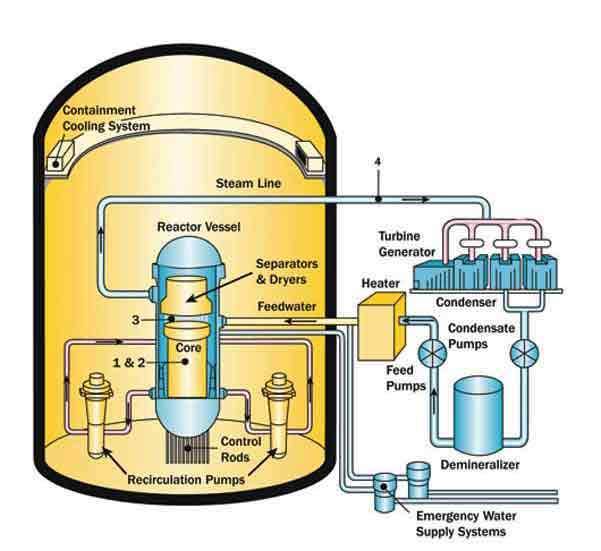
\includegraphics[width=\textwidth]{NRC-BWR.jpg}
 		    \caption{}
 		    \label{subfig:BWR}
 		\end{subfigure}
 		
		\begin{subfigure}[b]{0.65\textwidth}
 		    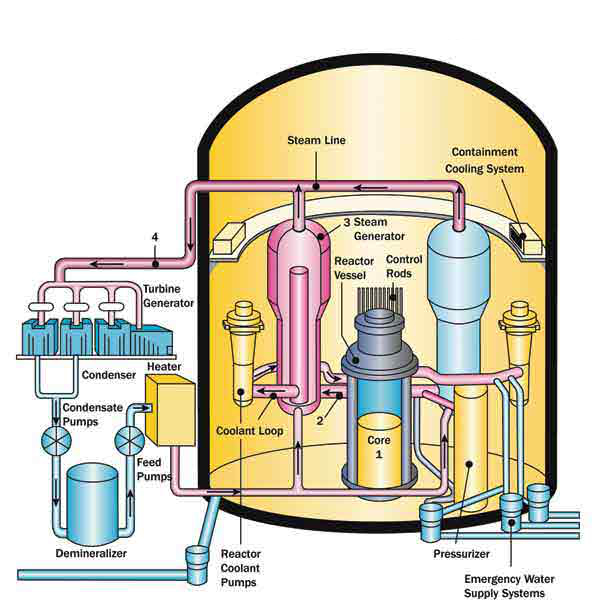
\includegraphics[width=\textwidth]{NRC-PWR.jpg}
 		    \caption{}
 		    \label{subfig:PWR}
 		\end{subfigure}
		\caption[Représentation schématique des technologies:
        a) réacteur à eau bouillante,
        b) réacteur à eau préssurisée.]
        {Représentation schématique des technologies:
        a) réacteur à eau bouillante,
        b) réacteur à eau préssurisée \citep{USNRC2013}.} 
 		\label{fig:Assembly_Control_Blades} 
 	\end{figure}
     \newpage


    

	
    \begin{table}[H]
        \begin{small}
        \centering
        \begin{tabular}{p{0.35\textwidth}p{0.28\textwidth}p{0.28\textwidth}}
        \toprule
        \textbf{Paramètres} & \textbf{REP} & \textbf{REB} \\ \midrule
        Fluide caloporteur & Eau pressurisée & Eau bouillante \\ \hline
        Matériaux des assemblages & Zy-4, Zirlo, Duplex, M5 & Zy-2, Zy-4 \\
                                    & Inconel, SS & Inconel, SS \\ \hline
        Flux de neutrons rapides ($\rm cm^{-2} \, s^{-1}$) &	\num{6}--\num{9e13} &	\num{4}--\num{7e13} \\ \hline
        Température (\si{\degreeCelsius}) & & \\
        Entrée & 279--294 & 272--278 \\
        Sortie & 313--350 & 280--300 \\ \hline
        Pression (bar) & 155--158 & 70--80 \\ \hline
        Vitesse du fluide caloporteur (\si{\meter\per\second}) & 3--6 & 2--5 \\ \hline
        Chimie du fluide caloporteur & & \\
        Oxygène  (\si{\ppb}) & <0.05 & 200--400 \\
        Hydrogène (\si{\ppm}) & 2--4 & 0.02 \\
        Acide borique (\si{\ppm}) & 0--2200 & -- \\
        LiOH (\si{\ppm}) & 0.5--3.5 & -- \\
        \bottomrule
        \end{tabular}
        \caption[Comparaison des paramètres de fonctionnement des technologies REB et REP.]%
        {Comparaison des paramètres de fonctionnement des technologies REB et REP \citep{Adamson2002}.}
        \label{tab:operating_parameters_reactors}
        \end{small}
    \end{table}

%%%%%%%%%%%%%%%%%%%%%%%%%%%%%%%%%%%%%%%%%%%%%%%%%%%%%%%%%%%%%%%%%%%%%%%%%%%%%%%%%%%%%
%%%%%%%%%%%%%%%%%%%%%%%%%%%%%%%%%%%%%%%%%%%%%%%%%%%%%%%%%%%%%%%%%%%%%%%%%%%%%%%%%%%%%
\section{Assemblage de combustible dans un REB}\label{sec:BWR_fuel_assembly}

    Les pastilles d’uranium sont empilées dans un crayon fermé hermétiquement qui
    les isole du fluide caloporteur comme illustré sur la figure \ref{fig:fuel_rod}.
    L’alliage de zirconium Zircaloy-2 est le matériau utilisé pour la fabrication
    des gaines de confinement.

    

    Ces crayons sont regroupés pour former un assemblage combustible dans lequel ils
    sont arrangés en réseau à maille carrée dans une structure assurant notamment
    leur maintien mécanique. Cet arrangement géométrique permet la circulation de
    l’eau entre les crayons et donc la dissipation de la chaleur
    engendrée dans le coeur du réacteur. L’assemblage de combustible est arrangé
    différemment par rapport à un REP à cause des variations de densité du fluide
    caloporteur. Les crayons sont regroupés dans des boîtiers carrés placés aux
    quatre coins de la croix de contrôle comme illustré sur la figure
    \ref{fig:Assembly_Control_Blades}.

    Les grilles de maintien permettent d’assurer la cohésion des crayons.
    Les matériaux généralement utilisés pour la fabrication des grilles de maintien sont des alliages de nickel 718 et
    X750.
    La croix de contrôle, généralement faite en acier
    inoxydable 316L, peut coulisser le long des assemblages de combustible afin
    d’assurer le contrôle de la fission de l’uranium en absorbant les neutrons. 

    Ces deux éléments, grilles de maintien et croix de contrôle, sont
    susceptibles d'induire le phénomène de Shadow Corrosion sur la gaine de confinement en
    Zircaloy-2. 
    Les paragraphes \ref{subsec:Zirconium} à \ref{subsubsec:Zircone} qui suivent donnent quelques informations sur les
    matériaux de gaine et l'oxyde qui se développe à leur surface.

    \newpage
    \begin{figure}[H] 
 		\centering 
 		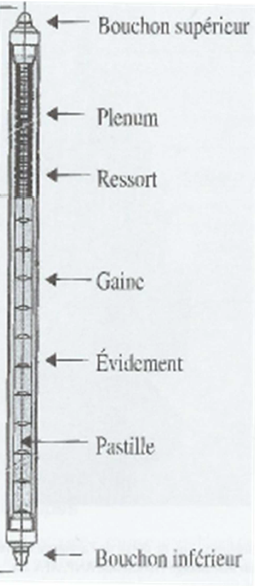
\includegraphics[height=0.40\textheight]{Buttin_2011-Fig1-1.png} 
 		\caption[Représentation schématique d'une gaine de confinement du combustible.]
        {Représentation schématique d'une gaine de confinement du combustible\citep{Coppolani2004}.} 
 		\label{fig:fuel_rod} 
 	\end{figure}

    \begin{figure}[H] 
 		\centering 
 		\begin{subfigure}[b]{0.45\textwidth}
 		    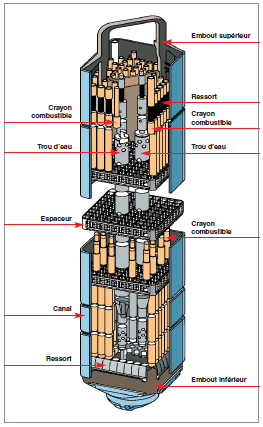
\includegraphics[width=\textwidth]{Pradel_2008-Fig91.png}
 		    \caption{}
 		    \label{subfig:BWR_fuel_assembly}
 		\end{subfigure}
 		\quad \quad \quad
		\begin{subfigure}[b]{0.45\textwidth}
 		    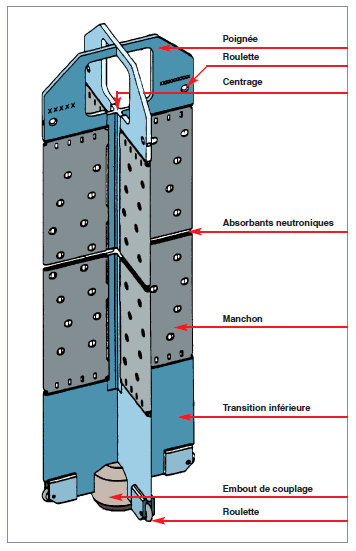
\includegraphics[width=\textwidth]{Pradel_2008-Fig92.png}
 		    \caption{}
 		    \label{subfig:COntrol_Blades}
 		\end{subfigure}
		\caption[Le combustible dans un réacteur à eau bouillante:
        a) assemblage de combustible,
        b) croix de contrôle.]{Le combustible dans un réacteur à eau bouillante:
        a) assemblage de combustible,
        b) croix de contrôle \citep{Pradel2008}.} 
 		\label{fig:Assembly_Control_Blades} 
 	\end{figure}
    \newpage

    
    
	 	
    \subsection{Zirconium pur}\label{subsec:Zirconium}

    Le zirconium répond au cahier des charges des gaines de confinement. En effet,
    ses propriétés physico-chimiques lui confèrent une bonne transparence aux
    neutrons, une bonne conductivité thermique, une bonne résistance mécanique, même
    à haute température et une bonne étanchéité entre les pastilles d'uranium et le fluide caloporteur.
    Les principales propriétés physiques du zirconium sont résumées dans le tableau \ref{tab:physical_properties_zirconium}. 

    Il faut noter que la principale raison du choix du zirconium réside dans sa
    faible section de capture des neutrons qui est environ 30 fois inférieure à celle
    des aciers inoxydables. Les caractéristiques
    métallurgiques du zirconium sont liées à sa forte réactivité avec l’oxygène, aux
    différentes interactions chimiques avec les éléments d’alliages (solubilité
    totale ou formation de phases intermétalliques) et à sa structure anisotropique
    hexagonale compacte qui conduit au développement d'un matériau texturé après
    traitement thermomécanique. 


    \begin{table}[H]
        \begin{small}
            \centering
            \begin{tabular}{p{0.45\textwidth} p{0.13\textwidth} p{0.13\textwidth} p{0.13\textwidth}}
                \toprule
                 & \textbf{Moyenne} & \textbf{Direction [1120]} & \textbf{Direction [0001]} \\ \midrule
                Masse volumique (\si{\kilogram\per\cubic\meter}) & 6500 & -- & -- \\ \hline
                Dilatation thermique (\si{\per\kelvin}) & \num{6.7e-7} & \num{6.7e-6} & \num{10.4e-6} \\\hline
                Module de Young (GPa) & -- & 99 & 125 \\\hline
                Paramètre de réseau (\si{\nano\meter}) & -- & a=0.323 & c=0.515 \\\hline
                Conductivité thermique (\si{\watt\per\meter\per\kelvin})  & 22 & -- & -- \\\hline
                Chaleur spécifique (\si{\joule\per\kilogram\per\kelvin}) & 276 & -- & -- \\\hline
                Section de capture de neutron \newline (1~barn= $10^{-28}m^2$) & 0.185 & -- & -- \\
                \bottomrule
            \end{tabular}
            \caption[Propriétés physique du zirconium.]{Propriétés physiques du zirconium \citep{IAEA1998}.}
            \label{tab:physical_properties_zirconium}
        \end{small}
    \end{table}

    
    

    A température ambiante, la forme allotropique stable du zirconium est hexagonale
    compacte avec un ratio c/a égale à 1.593. Les paramètres du réseau cristallin a
    et c ont pour valeur \SI{0.323}{\nano\meter} et  \SI{0.515}{\nano\meter},
    respectivement \citep{Douglass1971}. Les différences de dilatation thermique
    entre les directions a et c impliquent que le ratio c/a tend vers le ratio idéal (1.633)
    à plus haute température. Le zirconium fond à
    \SI{1860}{\degreeCelsius}, et par conséquent, il peut être considéré comme un
    métal modérément réfractaire.

    Lors des refroidissements après traitement thermique, le zirconium subit une transformation allotropique de la structure
    cubique centrée $\beta$ vers la structure hexagonale compacte $\alpha$.
    En fonction de la vitesse de refroidissement, la transformation peut être
    martensitique ou bainitique. L’épitaxie des plaquettes de la phase $\alpha$ sur
    les anciens grains de la phase $\beta$ conduit à une microstructure avec un
    ensemble d’orientations cristallographiques identiques à celles de la phase
    $\beta$ formant ainsi une microstructure à plaques parallèles. 

    

    \subsection{Alliage Zircaloy-2}\label{subsec:Zircaloy-2}

    La solubilité relative des différents éléments d’alliage dans les phases
    $\alpha$ et $\beta$ est un critère de premier ordre pour le choix des quantités à dissoudre
    et des traitements thermiques à effectuer. Le tableau
    \ref{tab:zircaloy_chemical_composition} liste les spécifications ASTM en termes de
    composition chimique des alliages Zircaloy-2. Les différentes nuances ont été développées 
    pour s'adapter aux différents REB mis en service.

    

    L’étain stabilise la phase $\alpha$ dans laquelle il se retrouve en solution
    solide. Il fut, originellement, ajouté afin de contrer les effets néfastes de
    l’azote en termes de résistance à la corrosion. Avec les améliorations des
    procédés de fabrication, il est maintenant possible de diminuer la teneur en
    étain, dont on notera qu'il a également un impact sur les propriétés mécaniques. 

    Le fer, le chrome et le nickel ont une solubilité très limitée dans la phase
    $\alpha$ et se retrouvent sous formes de précipités dans la matrice métallique.
    Deux types de précipités se forment: les phases de laves $\rm Zr(Fe,Cr)_2$ et
    les phases de Zintl $\rm Zr_2(Fe,Ni)$. La présence et la taille de ces
    précipités sont deux paramètres importants pour la résistance à la corrosion
    \citep{Barberis2005}. 

    \begin{table}[H]
        \begin{small}
        \centering
        \begin{tabular}{p{0.2\textwidth}%
                        p{0.12\textwidth}%
                        p{0.12\textwidth}%
                        p{0.12\textwidth}%
                        p{0.12\textwidth}%
                        p{0.12\textwidth}}
        \toprule
        \textbf{ASTM Ref.} & \textbf{Sn (\%wt.)} & \textbf{Fe (\%wt.)} & \textbf{Cr (\%wt.)} & \textbf{Ni (\%wt.)} & \textbf{O (ppm)} \\ \midrule
        R 60802 Zircaloy-2 & 1.2--1.7 & 0.07--0.20 & 0.05--0.15 & 0.03--0.08 & 1000--1400\\
        \bottomrule
        \end{tabular}
        \caption[Composition chimique (ASTM) de l'alliage Zircaloy-2.]{Composition chimique de l'alliage Zircaloy-2 \citep{IAEA1998}.}
        \label{tab:zircaloy_chemical_composition}
        \end{small}
    \end{table}



    \subsection{Zircone}\label{subsubsec:Zircone}

    Lors de l’exposition des gaines de confinement dans l’environnement d’un REB en fonctionnement,
    une couche d'oxyde de zirconium ($\rm ZrO_2$) se développe rapidement en
    surface \citep{Cox2011}. 
    La zircone existe sous trois variétés polymorphiques:
    \emph{monoclinique}, \emph{quadratique} et \emph{cubique}.
    Les mailles élémentaires sont
    illustrées sur la figure \ref{fig:Zirconia_allotropic_forms} alors que les domaines d’existence ainsi que les
    paramètres de maille sont résumés dans le tableau \ref{tab:zirconia_allotropic_forms}.
   

    Dans les conditions de pression et de température d’un REB, la phase stable de
    la zircone est donc la forme monoclinique. La différence de volume entre la
    maille de zircone monoclinique et la maille hexagonale compacte du zirconium métallique
    sous-jacent conduit à un ratio de Pilling-Bedworth de 1.56 dont la conséquence est
    la présence de contraintes de compression à l’interface métal/oxyde. Ces contraintes
    mécaniques ainsi que l'irradiation ou la présence des précipités peuvent favoriser
    la stabilisation de la phase quadratique à l'interface métal/oxyde \citep{IAEA1998}. 

    \begin{figure}[H] 
 		\centering 
 		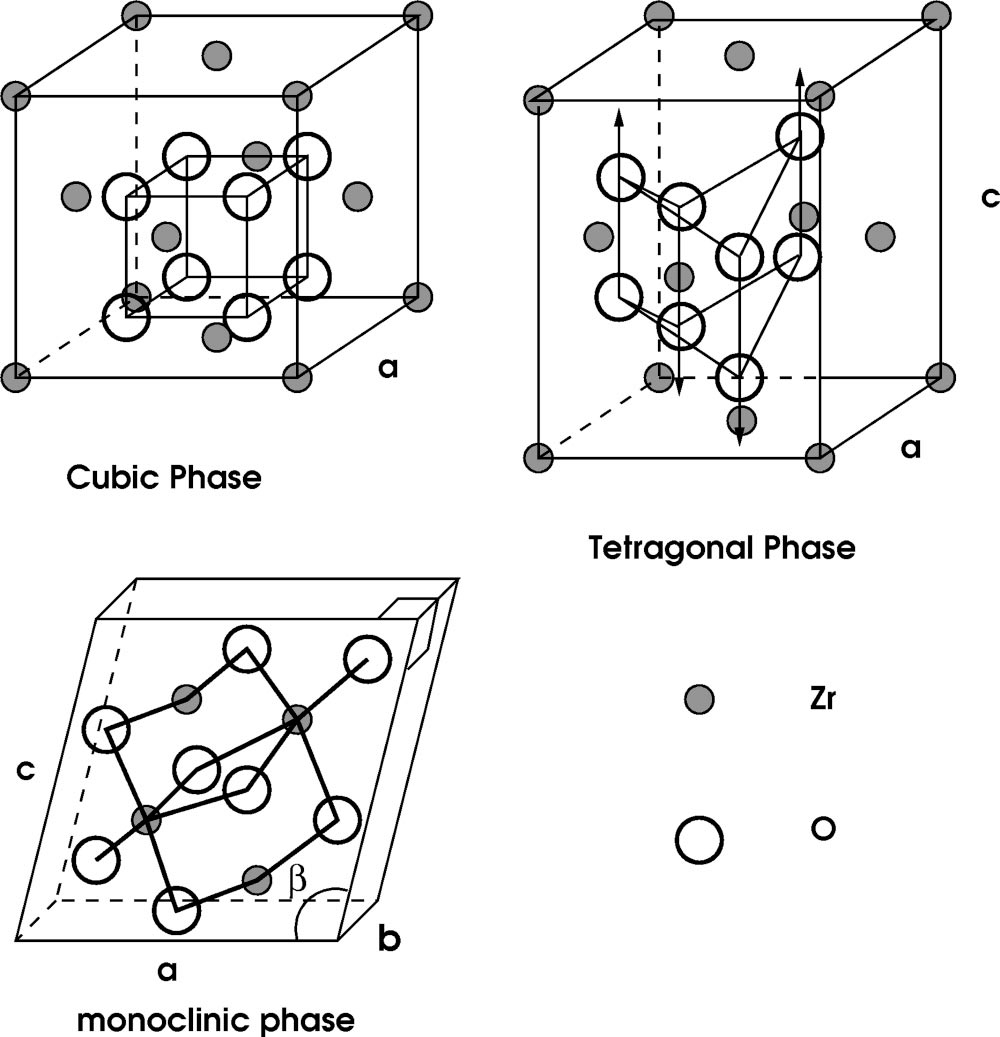
\includegraphics[width=0.59\textwidth]{Zhao_2002-Fig1.png} 
 		\caption[Les différentes phase de la zircone.]
        {Les différentes phases de la zircone \citep{Zhao2002}.
        Pour la phase quadratique (tetragonal en anglais), les flèches indiquent les distorsions du réseau par rapport à la phase cubique.} 
 		\label{fig:Zirconia_allotropic_forms} 
 	\end{figure}


    \begin{table}[H]
        \begin{small}
        \centering
        \begin{tabular}{p{0.30\textwidth} p{0.25\textwidth} p{0.35\textwidth}}
        \toprule
        \textbf{Variété polymorphique}    & \textbf{Température (°C)} & \textbf{Paramètre de maille (nm)} \\
        \midrule
        Monoclinique ($\rm m-ZrO_2$)      & T<1127    & a=0.510; b=0.516; c=0.527; $\beta$=99\si{\degree}21\si{\arcminute}      \\
        Quadratique ($\rm t-ZrO_2$)      & 1127<T<2297    & a=0.502; b=0.509 \\
        Cubique ($\rm c-ZrO_2$)      & 2297<T<2707    & a=0.503 \\
        \bottomrule
        \end{tabular}
        \caption[Domaine d'existence et paramètre de maille des variétés polymorphiques de la zircone.]
        {Domaine d'existence et paramètre de maille des variétés polymorphiques de la zircone \citep{Zhao2002}.}
        \label{tab:zirconia_allotropic_forms}
        \end{small}
	\end{table}

    Les propriétés d'isolant électrique de la zircone sont liées à la valeur de bande
    interdite élevée soit 5~eV \citep{Benaboud2007, Morrison1980}, mais sa résistivité varie sensiblement en présence
    d'impuretés.
    On considère généralement que la conductivité électrique et la conductivité ionique des couches d'oxydation du
    Zircaloy-2 sont séparées c'est-à-dire que la conductivité électrique est liées aux précipités alors
    que la conductivité ionique est liée aux défauts de la couche \citep{IAEA1998}. 

    Dans la suite du manuscrit, sauf indication contraire, les couches d'oxydation des alliages de zirconium seront
    dénommés \emph{couches de zircone}. 
    

	
\newpage
%%%%%%%%%%%%%%%%%%%%%%%%%%%%%%%%%%%%%%%%%%%%%%%%%%%%%%%%%%%%%%%%%%%%%%%%%%%%%%%%%%%%%
%%%%%%%%%%%%%%%%%%%%%%%%%%%%%%%%%%%%%%%%%%%%%%%%%%%%%%%%%%%%%%%%%%%%%%%%%%%%%%%%%%%%%
\section{Oxydation des alliages de zirconium}\label{sec:oxidation_zirconium}

    Dans un premier temps, la quantification de l'oxydation des alliages de zirconium est abordée en présentant la
    conversion des prises de masse en épaisseur de couche de zircone équivalente et en densité de courant d'oxydation équivalente. 
    Ensuite, l'analyse de l'oxydation hors irradiation
    permet de présenter les points clés en termes de cinétique, de porteurs de charge dans la couche de zircone et de
    processus limitant, complétée par une analyse de l'oxydation sous irradiation.

    \subsection{Quantifications de l'oxydation}\label{subsec:oxidation_introduction}


    Le diagramme de phase du système Zr/O est illustré en figure \ref{fig:ZrO_thermodynamics}. Il
    indique que tout l'oxygène n'est pas sous forme d'oxyde. Une partie de l'oxygène est dissoute
    dans la matrice $\alpha$ de zirconium. La proportion d'oxygène dissous est encore mal connue et elle dépend de
    l'équilibre entre les cinétiques d'oxydation et de dissolution. Tout changement de cinétique
    d'oxydation aura un impact sur l'extension spatiale de la zone de diffusion de l'oxygène dissous.
    Cependant, la quantité d'oxygène dissous est faible au regard de celle engagée dans les oxydes formés aux
    températures de fonctionnement d'un réacteur à eau bouillante.

    \begin{figure}[H]
    \centering
    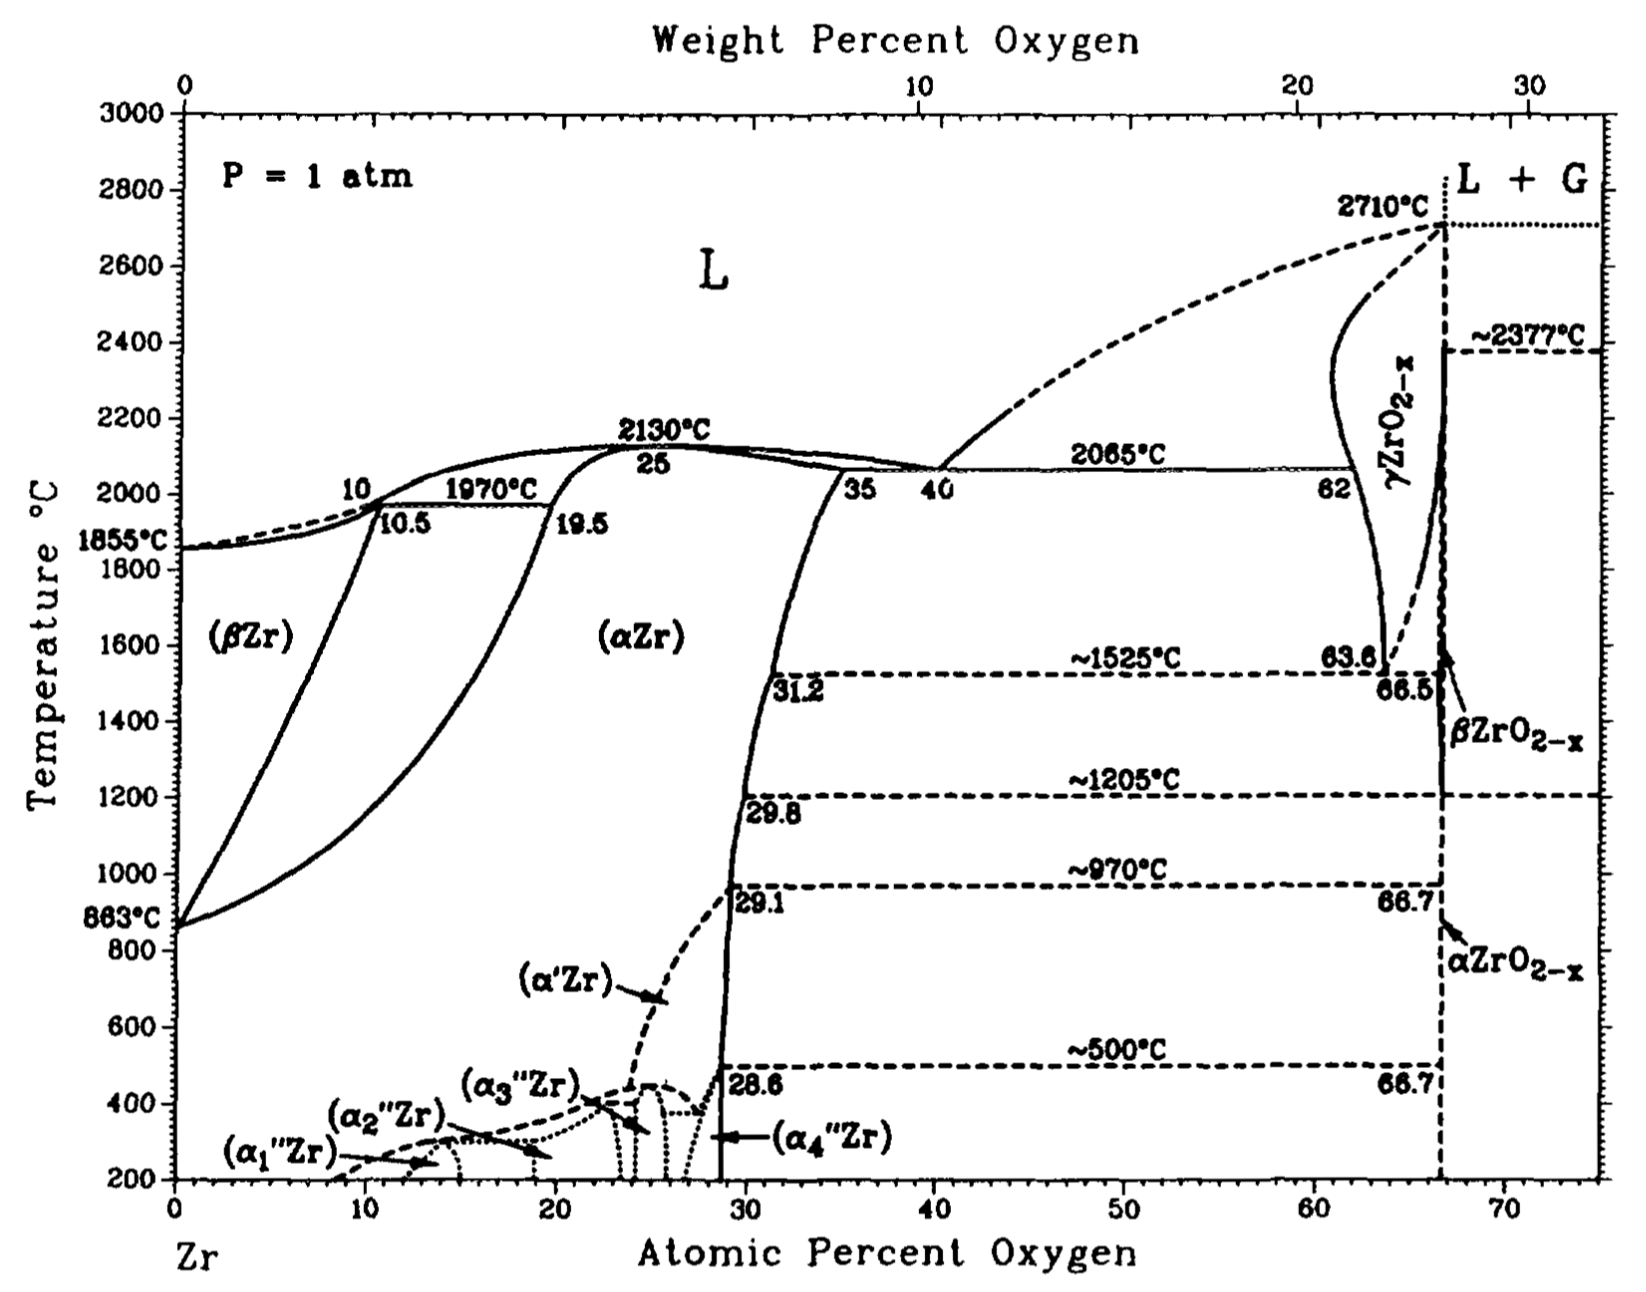
\includegraphics[width=0.85\textwidth]{IAEA_1998_Fig2_1a.png}
    \caption[Diagramme de phase du système ZrO/O]{Diagramme de phase du système Zr/O \citep{IAEA1998}.}
    \label{fig:ZrO_thermodynamics}
    \end{figure}

    Les cinétiques de croissance de l'oxyde sont donc généralement obtenues à partir des cinétiques expérimentales de prise de masse. L'hypothèse
    sous-jacente est que l'intégralité de la couche de zircone formée reste sur l'échantillon et que cette dernière est
    homogène sur l'ensemble de la surface exposée. Les cinétiques de prise de 
    masse sont converties en épaisseurs d'oxyde en utilisant la masse volumique théorique de $ZrO_2$ soit 
    \SI{5.68}{\gram\per\cubic\centi\meter} \citep{Lide2003}.
    %ce qui est une approximation car une partie des précipités
    %sont oxydés et bien d'avantage en raison de l'oxygène qui est dissout dans le métal sous-jacent.
    Le rapport de conversion de
    \SI{15}{\milli\gram\per\square\deci\meter} par micron d'épaisseur d'oxyde obtenue avec cette valeur de masse volumique
    reste une approximation, mais une utilisation standardisée permet  une première comparaison des
    cinétiques d'oxydation de différents alliages.

    Etant donné que le présent travail de thèse comporte une étude électrochimique de l'oxydation des alliages de zirconium, il est
    nécessaire de pouvoir convertir les cinétiques de croissance d'oxyde en densités de courant d'oxydation équivalentes.
    Sur la base des hypothèses formulées pour la conversion des prises de masse en épaisseur équivalente, il est
    possible de convertir une épaisseur d'oxyde en densité de courant
    d'oxydation en effectuant une approximation au premier ordre selon la loi de Faraday \citep{Bard2001}. Cette
    conversion est intéressante car la densité de courant, $j$, est une image de la vitesse d'oxydation.
    A partir des demi-réactions anodiques et cathodiques associées \citep{Adamson2007} à la corrosion du zirconium 
    (éq. \ref{eq:anodic_half_reaction} et \ref{eq:cathodic_half_reaction}),
    il est possible d'exprimer la densité de courant, j, en fonction de l'épaisseur de la
    couche de zircone, $d_{ZrO_2}$, par l'équation \ref{eq:th_to_j}. 



    \begin{equation}
        \text{Interface interne: }Zr_{metal} \rightarrow Zr_{Zr}^x + 4e^{-} + 2V_O^{\bullet \bullet}
        \label{eq:anodic_half_reaction}
    \end{equation}

    \begin{equation}
        \text{Interface externe: }2V_O^{\bullet \bullet} + 2 H_2O + 4e^{-}  \rightarrow 2O_O^x + 2H_2 \\
    \label{eq:cathodic_half_reaction}
    \end{equation}


    \begin{equation}
    \begin{split}
        \mathit{j} &= \frac{4F\rho _{ZrO_2}}{M_{ZrO_2}}\frac{d}{d\mathit{t}} \mathit{d_{\mathrm{ZrO_2}}}\\
        \mathit{j}[\si{\micro\ampere\per\square\centi\meter}] &\approx \num{1.78e6}
        \frac{d}{d\mathit{t}} \mathit{d_{\mathrm{ZrO_2}}} \frac{[\si{\micro\meter}]}{[\si{\second}]}
    \end{split}    
    \label{eq:th_to_j}
    \end{equation}


    \subsection{Oxydation hors irradiation}\label{subsec:no_irradiation}
    
    \subsubsection{Cinétiques d'oxydation}\label{subsubsec:oxidation_kinetics}
    
    Les expositions de Zircaloy-2 en milieu aqueux à différentes températures montrent que la cinétique d'oxydation du Zircaloy-2 est
    relativement lente en autoclave comme illustré sur la figure \ref{fig:Zy2_Kinetics_vs_T}, où les courbes à
    \SI{275}{\degreeCelsius} et \SI{300}{\degreeCelsius} sont représentatives des températures d'entrée et de sortie d'un
    réacteur à eau bouillante. Après un an d'oxydation en
    autoclave, la couche de zircone présente une épaisseur de seulement quelques microns. 

    La figure \ref{fig:Zy2_Kinetics_vs_T_J} montre en fonction du temps la densité de courant anodique obtenue par
    numérisation des données de
    la figure \ref{fig:Zy2_Kinetics_vs_T} et application de l'équation \ref{eq:th_to_j}. Dans les premiers instants de
    l'oxydation, la densité de courant est comprise entre 2 et 5 \si{\micro\ampere\per\square\centi\meter}, elle passe 
    rapidement sous le seuil de \SI{1}{\micro\ampere\per\square\centi\meter}, ainsi
    après 10 jours d'oxydation, la densité de courant vaut environ \SI{0.5}{\micro\ampere\per\square\centi\meter}, et après 50 jours,
    elle devient inférieure à \SI{0.1}{\micro\ampere\per\square\centi\meter} pour atteindre
    environ \SI{0.05}{\micro\ampere\per\square\centi\meter} après un an d'oxydation. Cette première analyse est certes
    simpliste mais elle fournit des ordres de grandeur pour les valeurs de densité de courant typiques qui seront
    mesurables en autoclave hors irradiation.

    \begin{figure}[H]
        \centering
        \begin{subfigure}[b]{0.65\textwidth}
            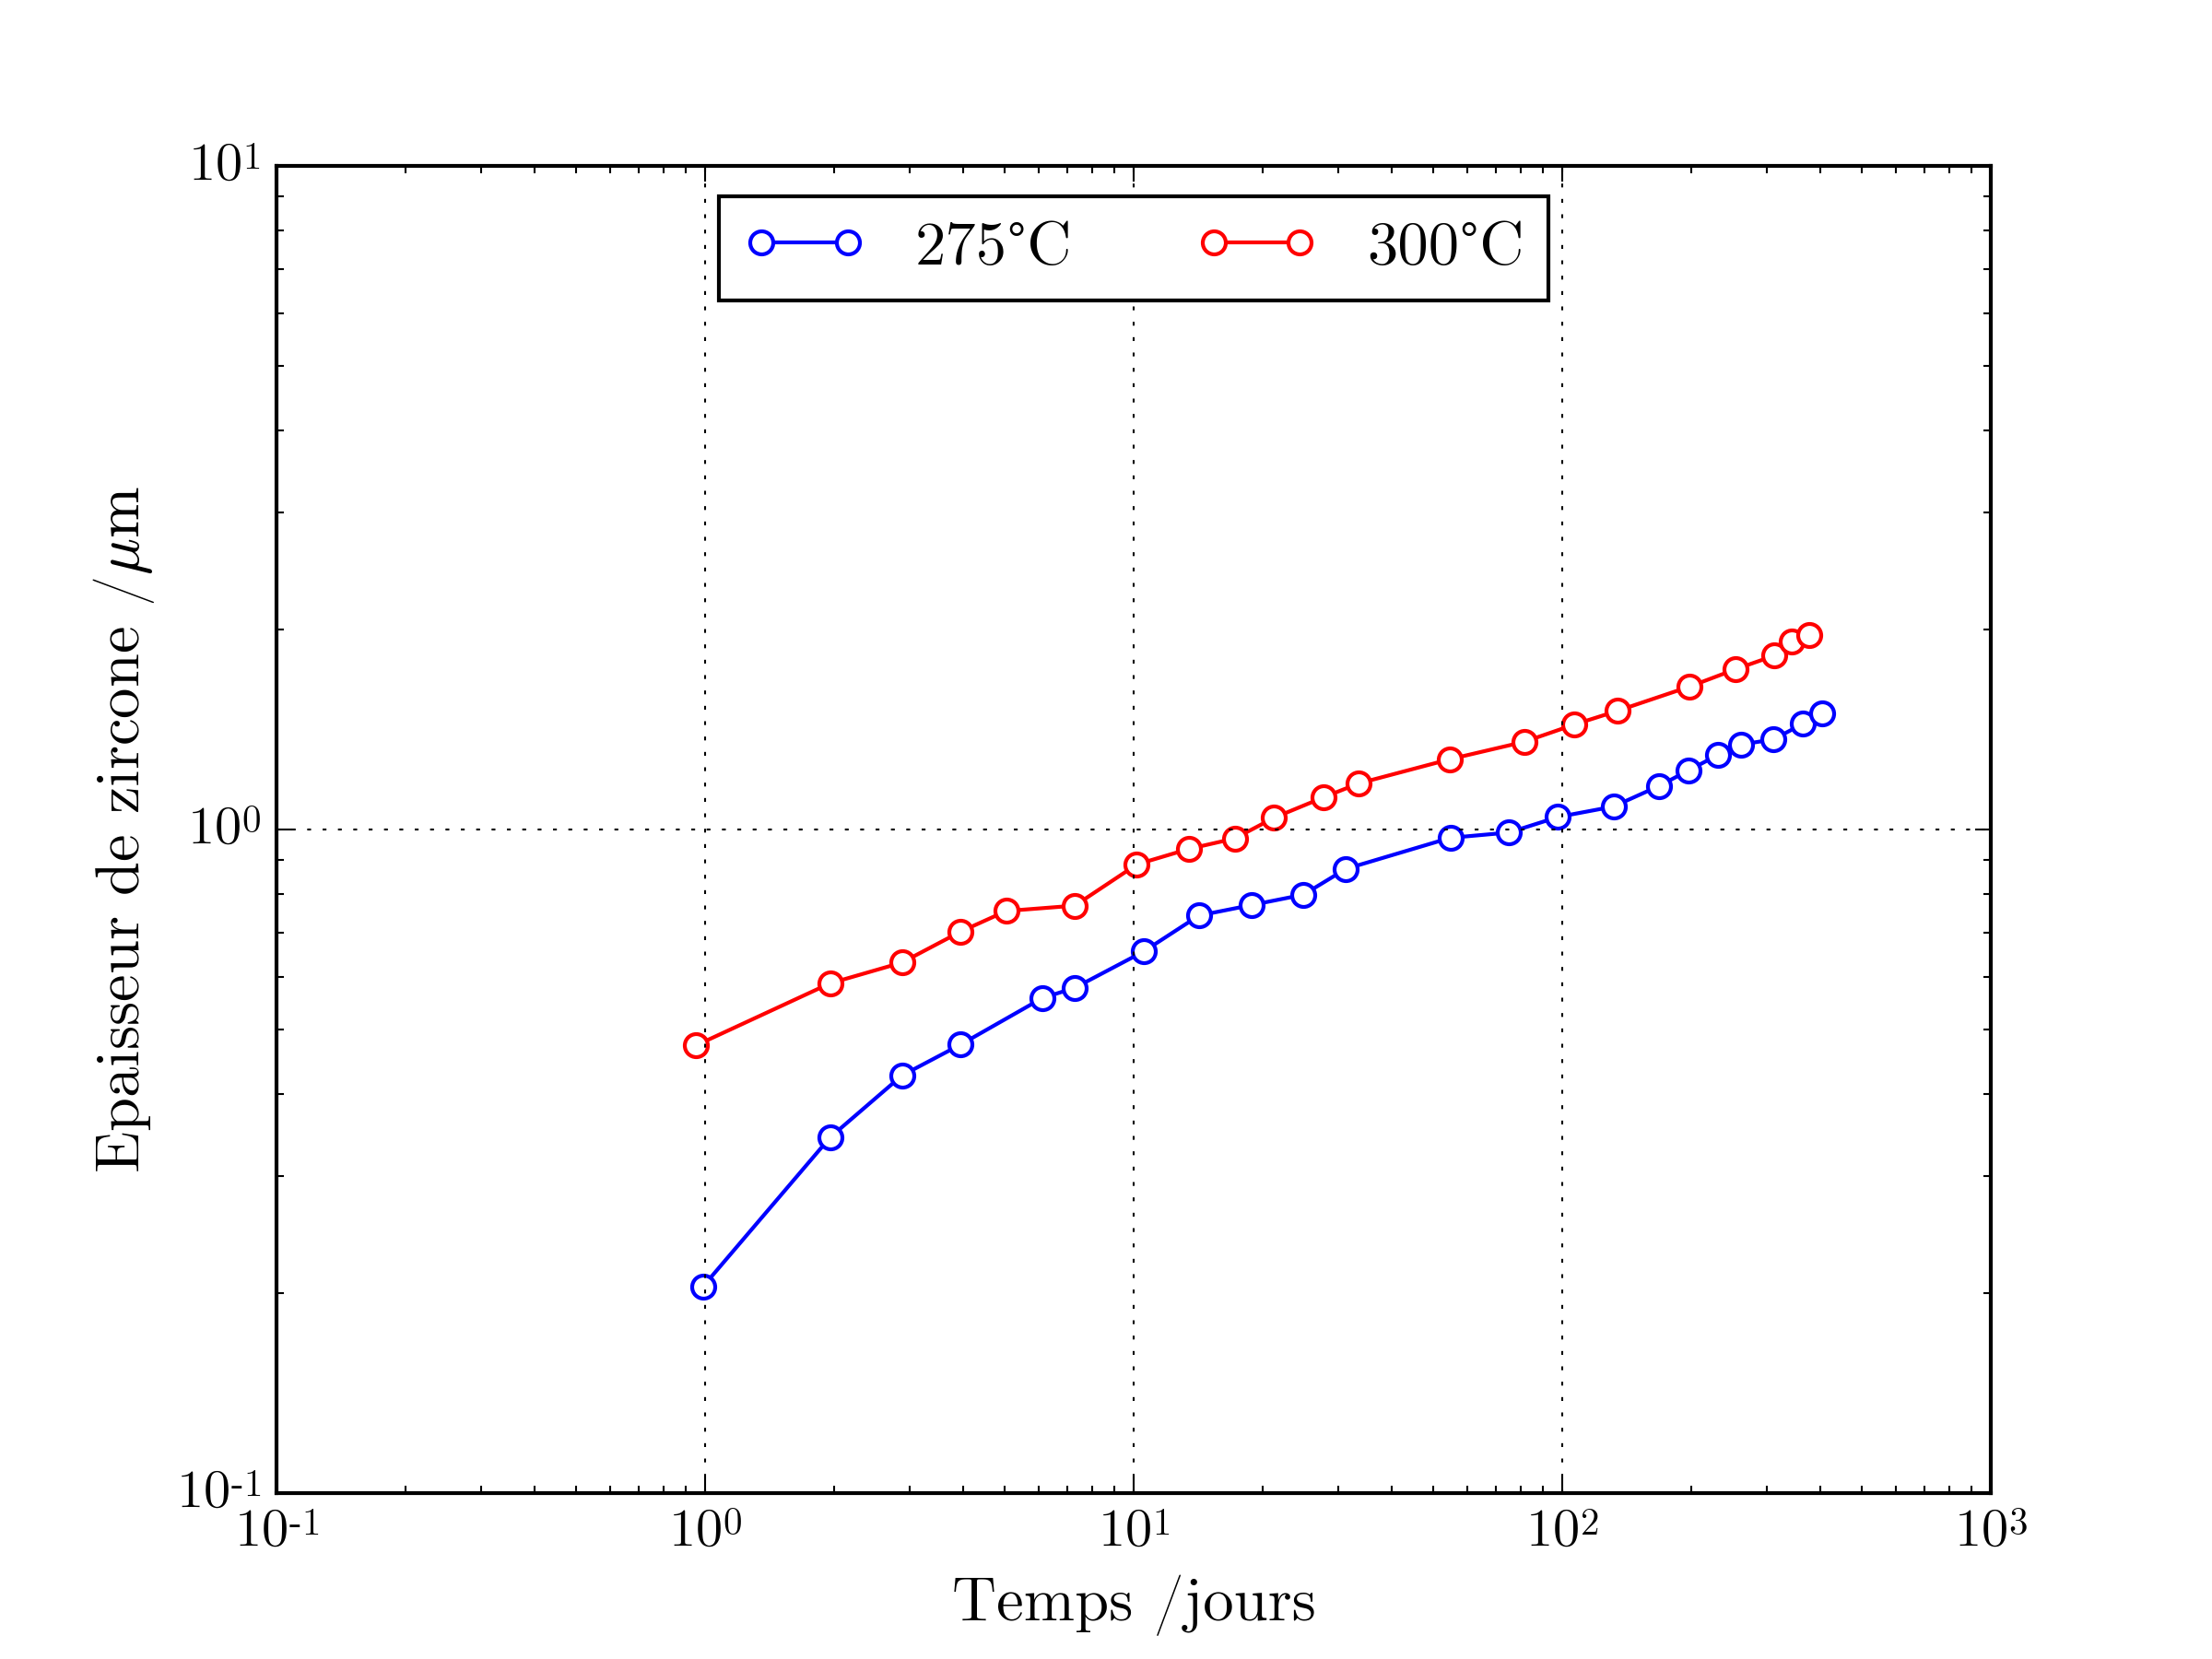
\includegraphics[width=\textwidth]{Cox_1968-Fig2-th.png}
            \caption{}
            \label{fig:Zy2_Kinetics_vs_T}
        \end{subfigure}
        \begin{subfigure}[b]{0.65\textwidth}
            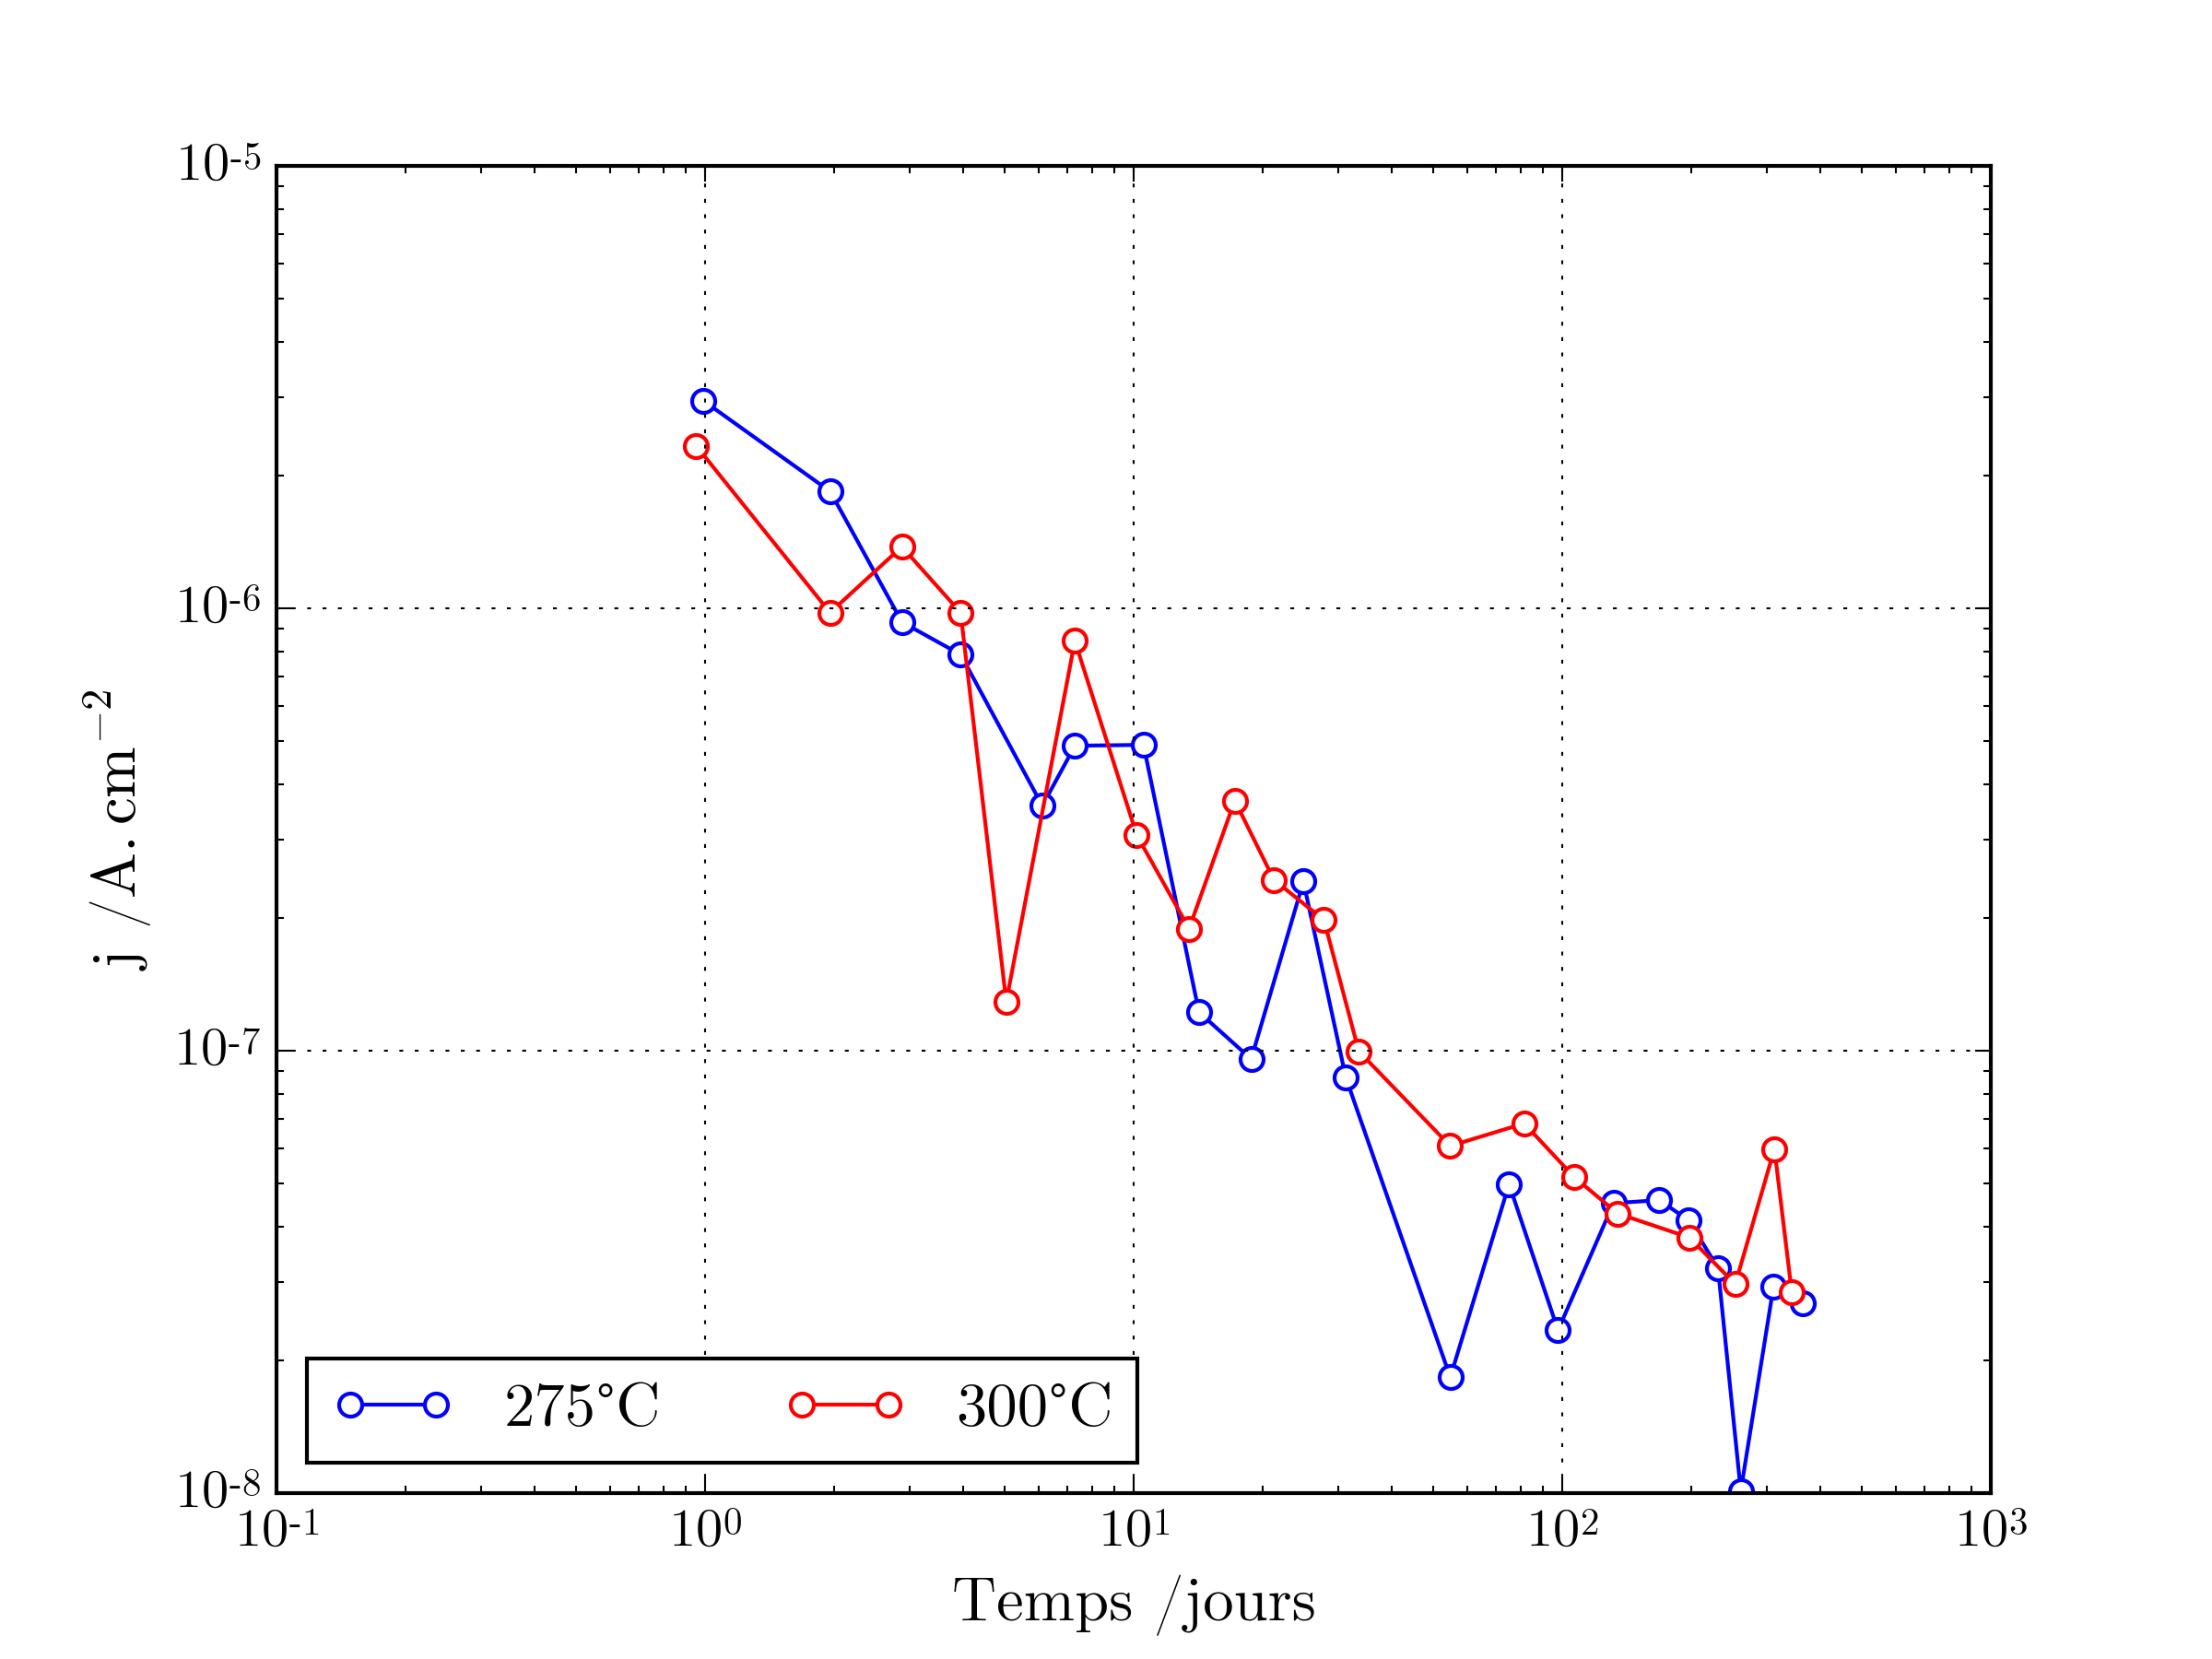
\includegraphics[width=\textwidth]{Cox_1968-Fig2-J.png}
            \caption{}
            \label{fig:Zy2_Kinetics_vs_T_J}
        \end{subfigure}
        \caption[Cinétique d'oxydation de l'alliage Zircaloy-2 en eau déminéralisée et désaérée à différentes
        températures.]{Cinétique d'oxydation de l'alliage Zircaloy-2 en eau déminéralisée et désaérée à différentes
        températures:
        a) évolution de la croissance de la couche de zircone \citep{Cox1968-1}, b) évolution de la densité de courant équivalente.}
        \label{fig:ch1_Zy2_Kinetics_th_J}
    \end{figure}


    La cinétique d'oxydation comporte deux régimes distincts (dits \emph{pré-transition} et \emph{post-transition}) séparés par
    une phase de \emph{transition}, comme illustré en figure \ref{fig:Zy2_Kinetics_Regimes}. 
    %La couche de zircone formée lors du 
    %régime de pré-transition est dense alors que la couche formée lors du régime de post-transition est poreuse
    %\citep{IAEA1998}. 
    La couche de zircone formée lors du régime de pré-transition est plus dense que la couche formée lors du régime de
    post-transition \citep{IAEA1998}.
    Généralement, la phase de \emph{transition} débute lorsque la couche de zircone atteint
    environ \SI{2}{\micro\meter}.

    Lors du régime de pré-transition, le profil cinétique d'oxydation est sub-parabolique, et non parabolique
    comme attendu pour une diffusion volumique de l’oxygène dans l’approximation de \citet{Wagner1933}.
    \citet{Dali2007} résume l'ensemble des lois cinétiques proposées pour le régime pré-transitoire avec 
    des descriptions mécanistiques particulières, qui ont été testées par
    ajustement aux données expérimentales. Par exemple, \citet{Smeltzer1961} proposent une loi cinétique basée sur la diffusion de
    l'oxygène aux joints de grain alors que \citet{Eloff1991} proposent un modèle où la cinétique est contrôlée par un
    champ électrique dans la couche de zircone en s'appuyant sur la théorie de \citet{Fromhold1980}. Par ailleurs,
    \citet{Cox1968-1} a montré par des
    expériences de marquage isotopique que la diffusion aux joints grains est nettement plus rapide que celle en volume.
    Il estime par conséquent que la vitesse est contrôlée par le transport de l’oxygène aux joints de grains. Comme la
    taille des grains augmente au cours de l’oxydation, cette croissance se traduit,
    d’après l’auteur, par une réduction sensible de la surface efficace de diffusion aux joints de grains et donc par
    une diminution de la vitesse par rapport à celle déduite de la loi parabolique.


            
    
    \begin{figure}[H]
        \centering
        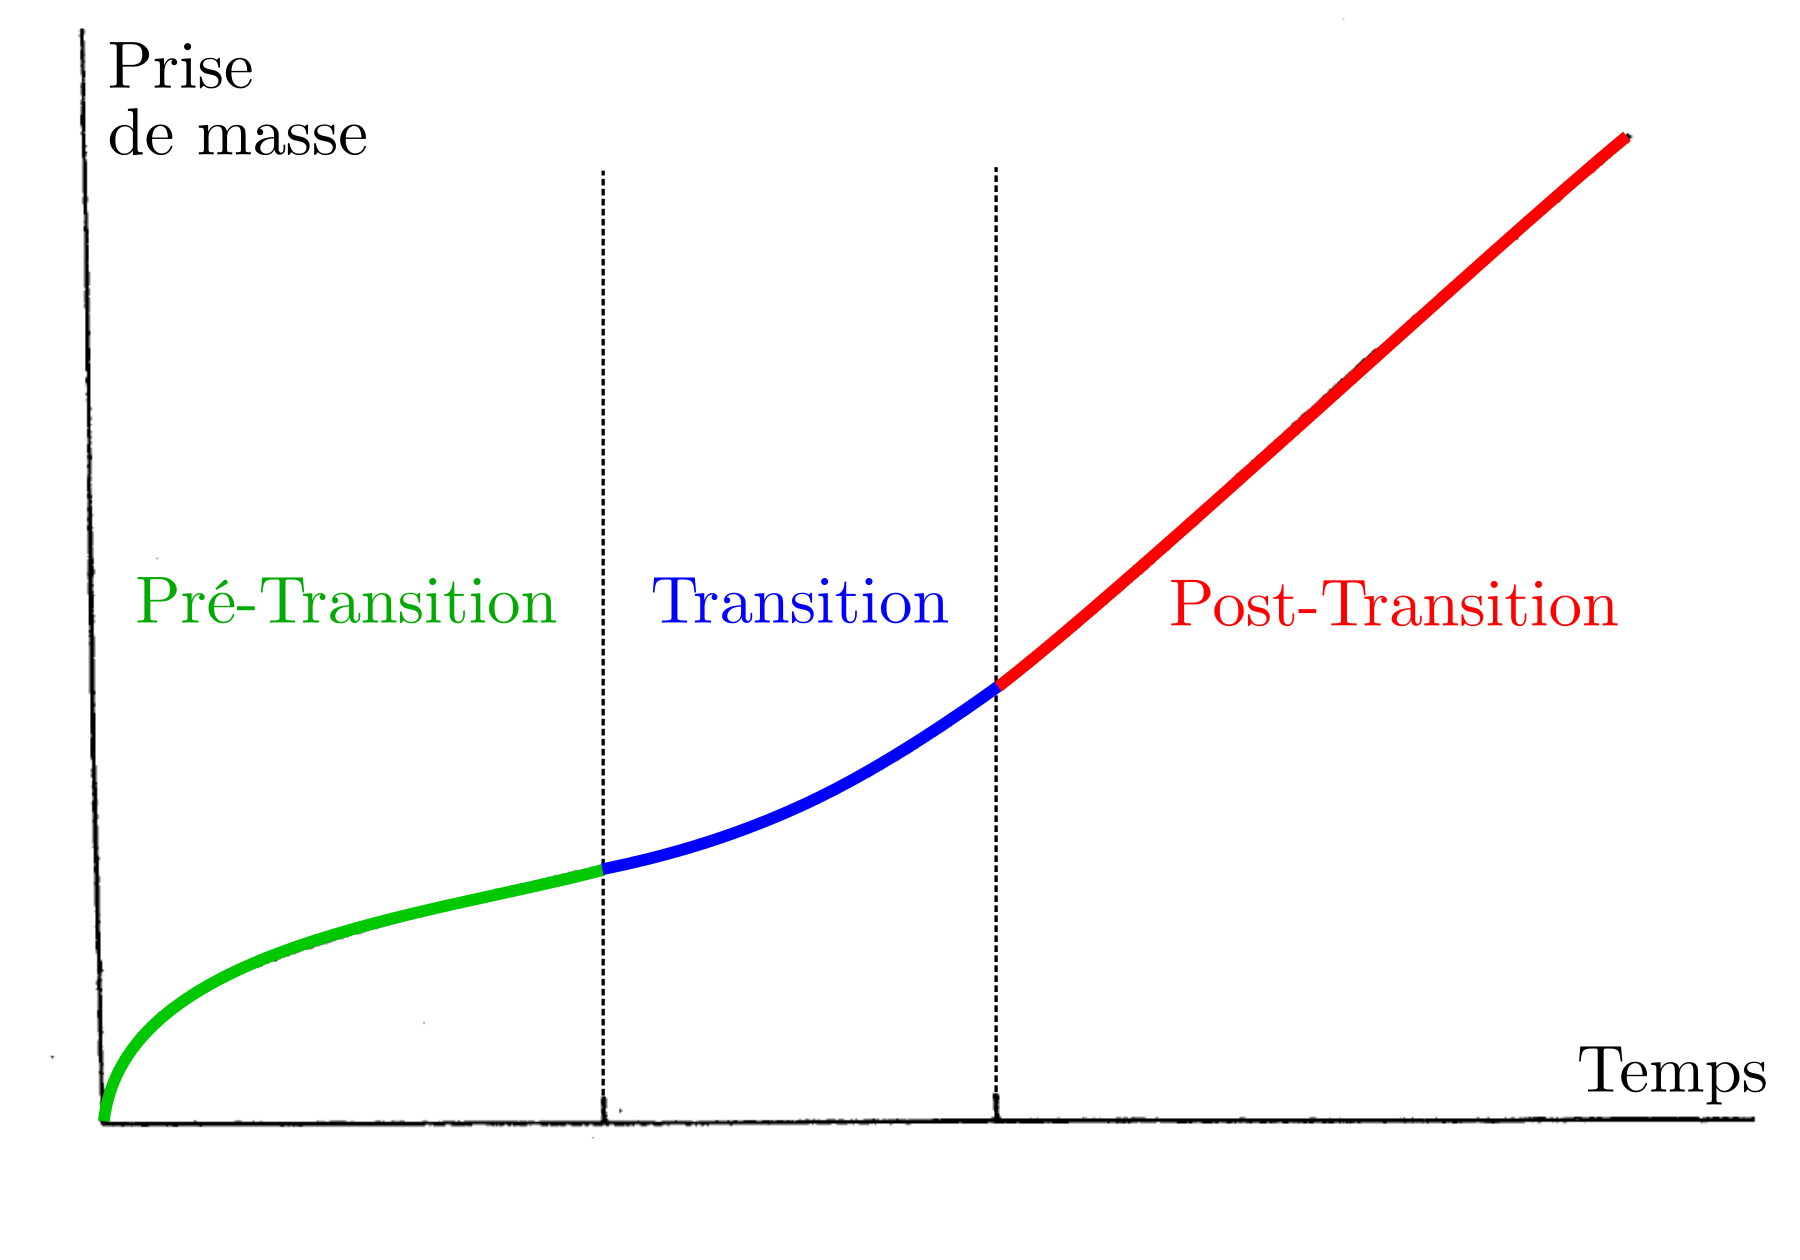
\includegraphics[width=0.65\textwidth]{Kinetics_Periods.png}
        \caption[Illustration des deux régimes de cinétique d'oxydation. Le deux régimes sont séparés par une phase de
        transition.]{Illustration des deux régimes de cinétique d'oxydation. Le deux régimes sont séparés par une phase de
        transition \citep{Cox2005}.}
        \label{fig:Zy2_Kinetics_Regimes}
    \end{figure}


    
    Comme déjà mentionné précédemment, la phase de transition apparaît lorsque l'épaisseur de la couche de zircone atteint
    environ \SI{2}{\micro\meter} \citep{IAEA1998}. Elle se traduit par l'apparition d'un changement de cinétique
    d'oxydation. La relaxation des contraintes dans la couche de zircone serait la première explication de la transition
    cinétique, en raison d'une
    fissuration (parallèle à l'interface) de la couche de zircone liée à des différences de contraintes dans l'épaisseur de l'oxyde.
    %La
    %différence de volume molaire entre le métal et la couche de zircone crée des contraintes de compression à l'interface
    %métal/oxyde alors que le rayon de courbure de la gaine crée des contraintes de traction à la surface externe de la couche de zircone,
    %favorables à l'initiation de fissures perpendiculaires à l'interface.
    %Cependant, les fissures perpendiculaires ne devraient pas se propager plus loin que l'axe des contraintes nulles laissant ainsi une
    %couche interne intacte. 
    La présence de fissures, perpendiculaires à l'interface, pénétrant jusqu'à l'interface métal/oxyde a été évoquée
    mais est encore débattue.
    La transition peut présenter différents mode de développement dans différentes conditions expérimentales
    \citep{Cox1968-1}. 
    Par exemple, en solutions aqueuses entre \SI{300}{\degreeCelsius} et \SI{360}{\degreeCelsius}, la transition peut être très
    soudaine, impliquant une forte augmentation de la cinétique d'oxydation. Pour des températures plus élevées, en présence
    de vapeur d'eau et d'oxygène, la transition est plus douce.
    %Enfin, une transition de type para-linéaire caractérisée par un changement de cinétique d'oxydation
    %constant de la cinétique sub-parabolique vers la cinétique linéaire en passant par la cinétique parabolique sans aucune accélération de la cinétique
    %d'oxydation.  
    
    Le profil cinétique d'oxydation du régime post-transition est, suivant les auteurs, soit un profil
    ressemblant à une succession de régimes de pré-transition dont l’amplitude diminue avec le temps
    \citep{Garcia1999}, soit un profil cinétique linéaire \citep{Vermoyal2002}. La différence entre ces deux profils dépend des
    conditions d’oxydation et des nuances d’alliage considérées.

    

    \subsubsection{Porteurs de charge dans la couche de zircone}\label{subsubsec:charge_carrier}

    En l'abscence de potentiel appliqué à l'échantillon, le courant d'oxydation correspondant à la demi-réaction anodique et le courant de réduction
    correspondant à la demi-réaction cathodique qui sont égaux et de signe opposé. Si cette condition d'électroneutralité n'est pas
    respectée dans les premiers instants de la formation de la couche de zircone, une différence de potentiel apparaît dans
    la couche de zircone entre l'interface métal/oxyde et l'interface oxyde/environnement dont l'effet est d'égaliser ces
    deux courants \citep{Cox1969}. La diffusion cationique (ions $Zr^{4+}$) est quasi inexistante dans la couche de
    zircone et seule
    la diffusion anionique (ions $O^{2-}$) a lieu au niveau des joints de grain possédant une concentration élevée de
    lacunes \citep{Cox1968-1,Brossmann1999}. Le transport dans la couche de zircone est de type lacunaire c'est-à-dire que des
    lacunes sont crées à l'interface métal/oxyde et diffusent vers l'interface oxyde/environnement. 

    Par conséquent, si les ions oxygène sont les seules espèces ioniques mobiles, l'électroneutralité dans la couche
    d'oxyde peut seulement être respectée avec un flux d'électrons dans le sens opposé. Le transport des électrons a
    probablement lieu par saut entre les atomes immobiles de Zr de la couche de zircone. Les phases intermétalliques,
    $Zr(Fe,Cr)_2$ et $Zr_2(Fe,Ni)$ dans la couche de zircone, sont potentiellement des sites de conduction électronique pour les électrons
    \citep{IAEA1998}.
    \citet{Sundell2012} ont récemment montré que le transport des électrons peut être favorisé par la ségrégation de Fe et
    de Ni aux joints de grain de la couche de zircone. Sur la base des ces résultats, la présence des phases intermétalliques peut
    paraître néfaste en termes de résistance à la corrosion. Cependant, la relation entre la présence des phases
    intermétalliques et la résistance à la corrosion n'est pas aussi tranchée. En effet, \citet{Barberis2005} ont 
    montré qu'un zirconium sans les précipités (dans le métal) avait une très faible résistance à la corrosion sous eau, par rapport à
    un zirconium contenant des précipités.  
     

    \citet{Shirvington1970-1} a étudié l'effet sur la conductivité de la couche de zircone des conditions
    oxydantes lors de sa formation. Il propose trois modèles de structure de couche de zircone en surface de phases intermétalliques dans
    l'alliage Zircaloy-2 comme illustré sur la figure \ref{fig:shirvington_oxide_structures}. Les modèles proposés ici sont
    basés sur l'analyse de courbes de polarisation mesurés en milieu sel fondu.

    Le modèle (i) correspond à la situation où le métal est à un potentiel très cathodique. Dans ce cas, les
    éléments plus nobles tels que Fe, Cr et Ni ne s'oxydent pas ou peu, avec pour conséquence la formation d'une couche
    de zircone non dopée. Les oxydes formés en milieu aqueux désaéré sont susceptibles de développer ce genre de
    structure.

    Le modèle (ia) est une structure
    supplémentaire pouvant apparaître dans les premiers instants de l'oxydation dans un environnement favorisant la
    cristallisation de magnétite $Fe_3O_4$ présentant une semi-conduction de type \emph{p}. L'augmentation de conductivité
    électronique peut être liée à l'injection de trou provenant de la bande de valence de la magnétite dont la
    conséquence sur les courbes de polarisation est de faciliter la demi-réaction cathodique

    Le modèle (ii) correspond à la situation où le métal est à un potentiel élevé, soit en raison d'un couplage, soit
    que la différence de potentiel dans la couche de zircone soit faible.
    Les
    éléments Fe, Ni, Cr peuvent alors se dissoudre dans la matrice de zircone et doper cette dernière. La présence d'hématite,
    présentant une semi-conduction de type \emph{n}, en
    surface n'est pas à exclure. Les oxydes formés en milieu aqueux oxygéné peu conducteur sont susceptibles de
    développer ce type de structure. Cependant, les courbes de polarisation mesurées montre un faible impact sur la
    conductivité électronique. L'ensemble de la structure peut être considéré comme un oxyde ayant une semi-conduction
    de type \emph{n}.


    Le modèle (iii) correspond à une situation intermédiaire entre le modèle (ia) et (ii). Ce modèle est envisageable
    lorsque le potentiel du métal se trouve à une valeur intermédiaire en milieu aqueux
    oxygéné. L'élément Fe (éventuellement Cr et Ni) peut se dissoudre dans la matrice de zircone, dopant cette
    dernière comme dans le modèle (ii). La diffusion jusqu'à l'interface externe pour former de la magnétite
    est éventuellement possible (modèle (ia)). Une partie de la magnétite est convertie en hématite. La conductivité
    électronique de la couche de zircone peut être liée à l'injection de trous provenant de la bande de valence de la
    magnétite. Il faut noter qu'un alignement adéquat des bandes de valence et de conduction, selon que les oxydes sont
    en appauvrissement
    ou en accumulation de porteurs de charge majoritaires, ainsi que des largeurs de bande interdite particulières 
    sont nécessaires pour qu'un tel agencement de couches
    semi-conductrices puissent générer un effet fort sur la conductivité électronique \citep{Gerischer1985}.

    
    \begin{figure}[H]
        \centering
        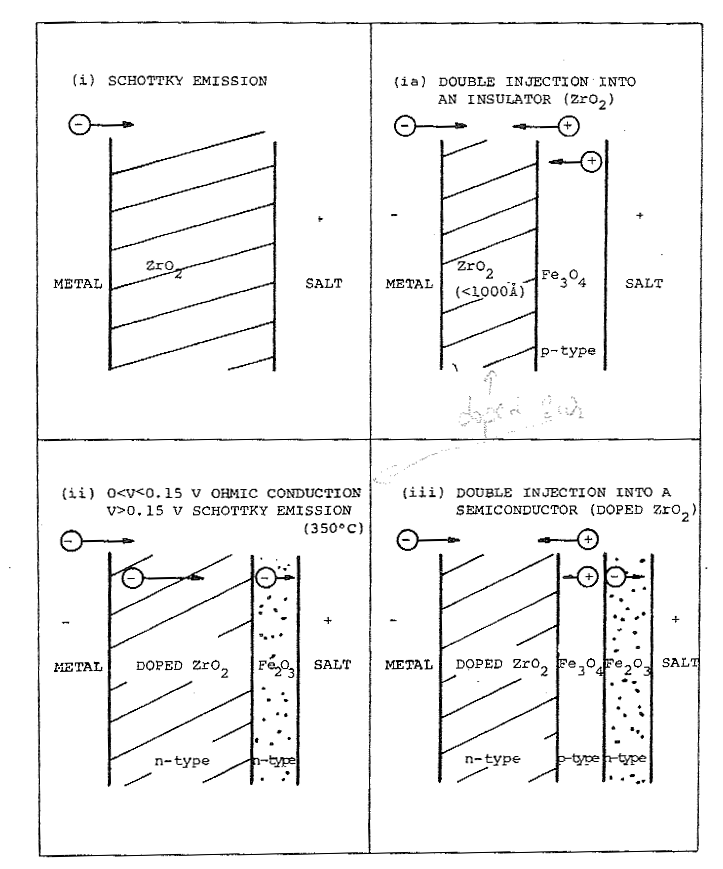
\includegraphics[width=0.9\textwidth]{Shirvington_1970-Fig12.png}
        \caption[Modèles de couche de zircone sur les phases intermétalliques de l'alliage Zircaloy-2.]{Modèles de couche
        d'oxyde sur les intermétalliques de l'alliage Zircaloy-2 \citep{Shirvington1970-1}.}
        \label{fig:shirvington_oxide_structures}
    \end{figure}

    L'auteur insiste sur le fait que la présence de l'oxygène ainsi que le potentiel du métal ont un effet fort sur la
    conductivité de la zircone lorsque de la magnétite peut cristalliser en surface. En effet, le fluide caloporteur
    d'un REB contient très souvent du fer sous forme ionique provenant des pièces de structure de la cuve
    \citep{IAEA1993, IAEA1998, IAEA2011}. Cependant, les dépôts de couleur rouge/orange (appelés CRUD) habituellement observés en
    réacteur sont majoritairement composés d'hématite \citep{Edsinger2004}.
    
    Enfin, l'auteur rappelle que
    l'accélération de la cinétique d'oxydation ne dépend pas seulement de la conduction électronique mais également du
    transport de matière dans la couche de zircone.      
   
   
   
    \subsubsection{Processus limitant}\label{subsubsec:rate_limiting}
         
    La détermination du processus limitant sur la base de mesures séparées des coefficients de diffusion de l'oxygène et de la
    conductivité électronique de la couche de zircone n'est pas simple à réaliser. Comme mentionné précédemment, les deux
    processus sont en balance. Dans le cas où les deux processus n'évoluent pas à la même vitesse dans les
    premiers instants de l'oxydation, une différence de potentiel apparaît entre l'interface interne et l'interface
    externe. Cette dernière accélère le processus le plus lent et ralentit le plus rapide. Les courbes de polarisation
    anodiques et cathodiques permettent d'avoir une estimation du processus limitant dans des conditions expérimentales
    données.

%    Mesurer le potentiel qui apparaît dans la couche d'oxyde n'est simple à réaliser sans perturber la réaction
%    d'oxydation. La figure \ref{fig:potential_drop_Zy2} montre les mesures expérimentales obtenues par \citet{Cox1969}
%    en bain de sel fondu sur du Zy2. Le potentiel à l'interface métal/oxyde diminue vers de potentiel plus cathodiques
%    lors des premiers instants de la croissance de la couche d'oxyde. Cette diminution a été attribuée à la formation d'oxyde de fer en
%    surface des intermétalliques \citep{Shirvington1970, Shirvington1970-1}.

%    \begin{figure}[!htb]
%        \centering
%        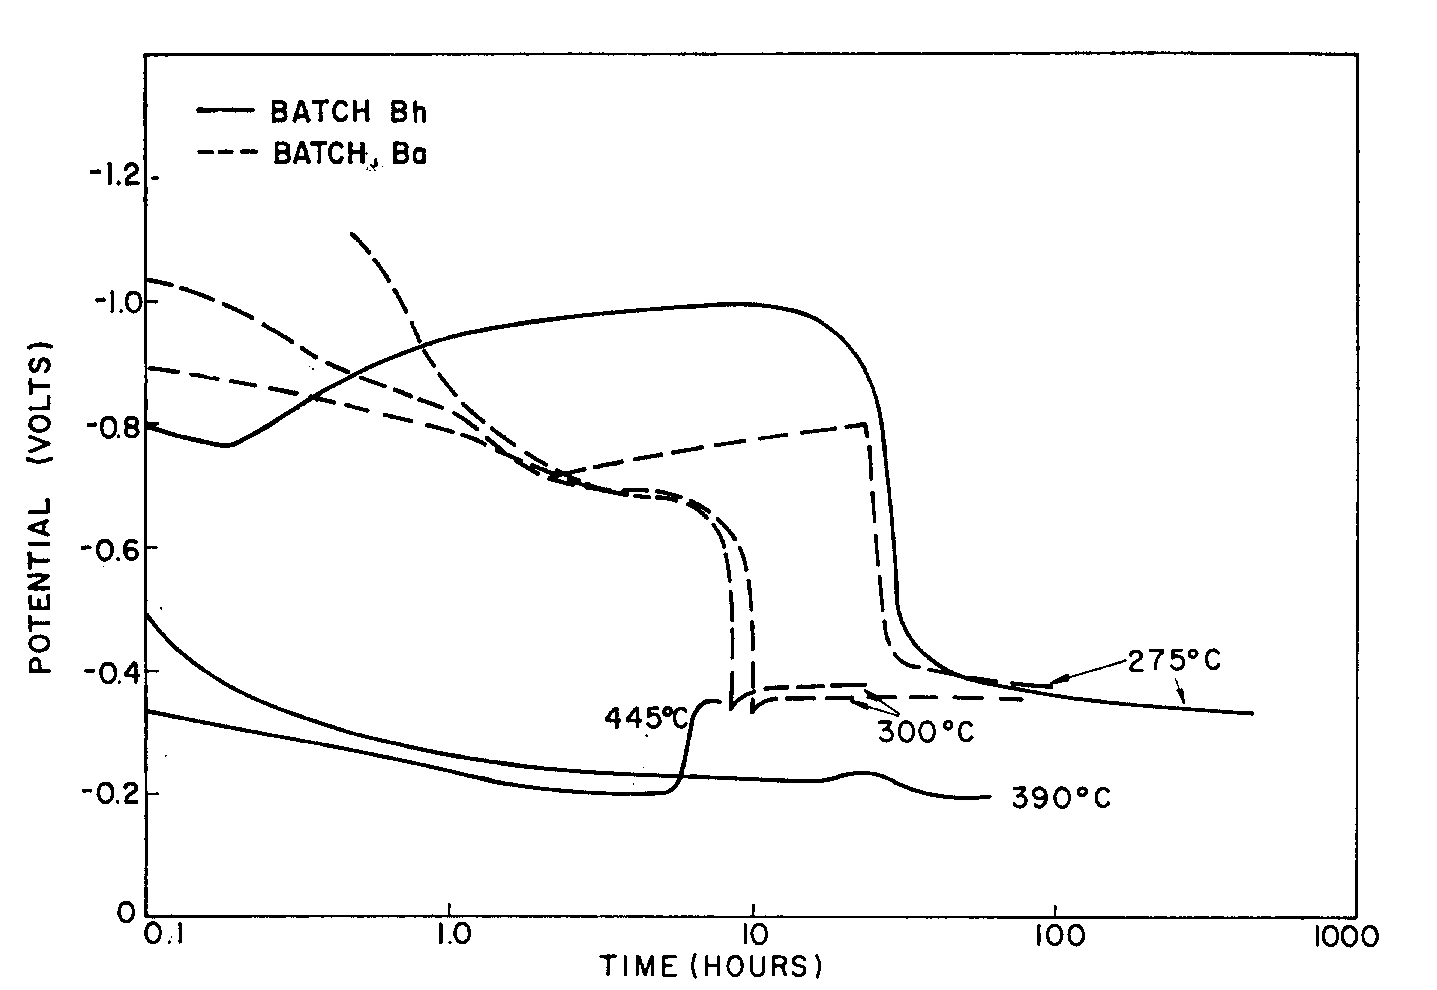
\includegraphics[width=0.45\textwidth]{Cox_1969-Fig4.png}
%        \caption[Evolution du potentiel de l'alliage Zircaloy-2 en bain de sel fondu.]{Evolution du potentiel de l'alliage
%    Zircaloy-2 en bain de sel fondu \citep{Cox1969}.}
%        \label{fig:potential_drop_Zy2}
%    \end{figure}


    Il est fort probable que la conduction électronique pilote la cinétique d'oxydation dans les premiers instants de la
    croissance de la couche de zircone. Cette dernière semble devenir plus conductrice à cause de la contribution des
    phases intermétalliques. Lorsqu'une certaine épaisseur d'oxyde est atteinte, les résistivités électronique et
    ionique semblent plus équilibrées.  La figure \ref{fig:oxide_film_diagram} schématise les différents processus
    intervenants dans l'oxydation de l'alliage Zircaloy-2 au niveau de la couche de zircone lors du régime de
    pré-transition. Cette figure met en lumière la dualité du transport ionique et du transport électronique qui
    doivent être en équilibre afin de maintenir l'électroneutralité dans la couche de zircone.
    
    \begin{figure}[H]
        \centering
        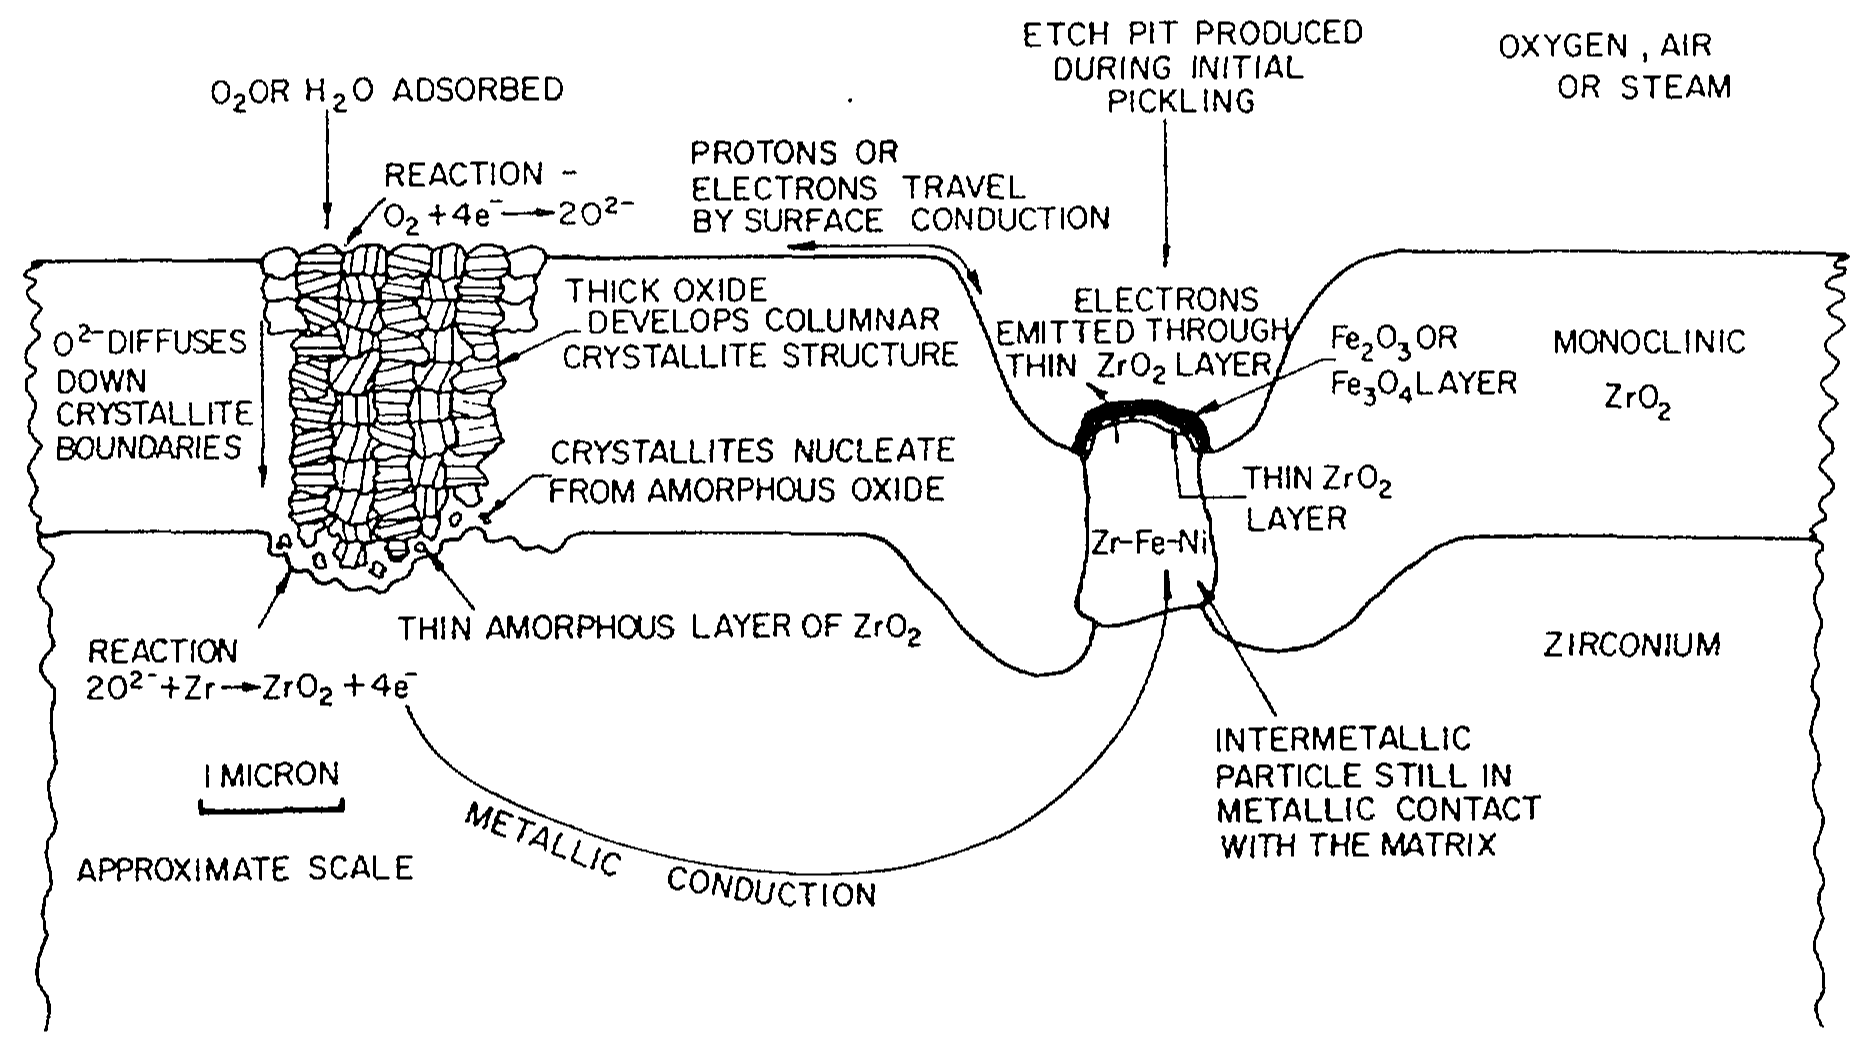
\includegraphics[width=0.95\textwidth]{IAEA_1993_Fig2_17.png}
        \caption[Représentation schématique de la couche de zircone se formant sur l'alliage Zircaloy-2 et des différents
    processus se déroulant lors de l'oxydation.]{Représentation schématique de la couche de zircone se formant sur
    l'alliage Zircaloy-2 et des différents processus se déroulant lors de l'oxydation \citep{IAEA1998}.}
        \label{fig:oxide_film_diagram}
    \end{figure}


    \subsection{Oxydation sous irradiation}\label{subsec:with_irradiation}

    L'impact de l’irradiation sur la cinétique l'oxydation du zirconium n'est pas encore parfaitement connu
    \citep{IAEA1998}. Cependant, un certain nombre de résultats expérimentaux sont disponibles et permettent d'avoir un aperçu de
    l'effet de l'irradiation. 
    
    En première approximation, l'irradiation des matériaux présente dans un coeur de réacteur est due à deux
    types de rayonnements: un rayonnement \emph{neutronique} et un rayonnement électromagnétique $\gamma$, s'y ajoute le
    rayonnement \emph{Cherenkov}, un rayonnement électromagnétique secondaire dans le domaine des UV. 
    Ce rayonnement est liée aux électrons produits par la diffusion de \emph{Compton} des rayonnements $\gamma$ sur les
    matériaux de structure. 
    
    L'irradiation par des neutrons rapides favorise la dissolution des phases intermétalliques et ainsi redistribue les
    éléments d'alliage dans la matrice $\alpha$ \citep{Vizcaino2008, Garzarolli2002}. 
    Cette dissolution est susceptible de doper la couche de zircone qui va se former autour des phases intermétalliques,
    ce qui peut induire une augmentation de la conduction
    électronique comme suggéré dans le paragraphe \ref{subsubsec:charge_carrier}.
    
    Travailler en laboratoire avec des rayonnements
    neutroniques nécessitent des moyens lourds et coûteux. On simule quelquefois l'effet d'une
    irradiation neutronique en la remplaçant par des atomes lourds tels que le xénon.
    \citet{Bererd2005} ont irradié une couche de zircone avec des atomes de Xe  
    ayant une énergie de 64.5 MeV et un flux de \SI{2.6e10}{\per\square\centi\meter\per\second}. La figure
    \ref{fig:Bererd_diffusion_increase} montre que l'irradiation peut engendrer une augmentation du coefficient de
    diffusion de plusieurs ordres de grandeur à \SI{300}{\degreeCelsius}. Cependant, il ne semble pas y avoir peu de preuves
    définitives d'un lien direct entre l'accélération de la cinétique de corrosion et l'augmentation des coefficients de
    diffusion de l'oxygène dans la couche de zircone \citep{IAEA1993, IAEA1998}.
    \citet{Simeone2000, Simeone2002} ont mis en évidence des
    changements de phase locaux dans la couche de zircone lorsque celle-ci est irradiée avec des atomes de Xe.
    L'irradiation avec des particules lourdes crée des défauts dans la couche favorisant la stabilisation de la phase
    quadratique. Cette transformation s'accompagne d'une augmentation des contraintes dans la couche
    de zircone.

    \begin{figure}[H]
        \centering
        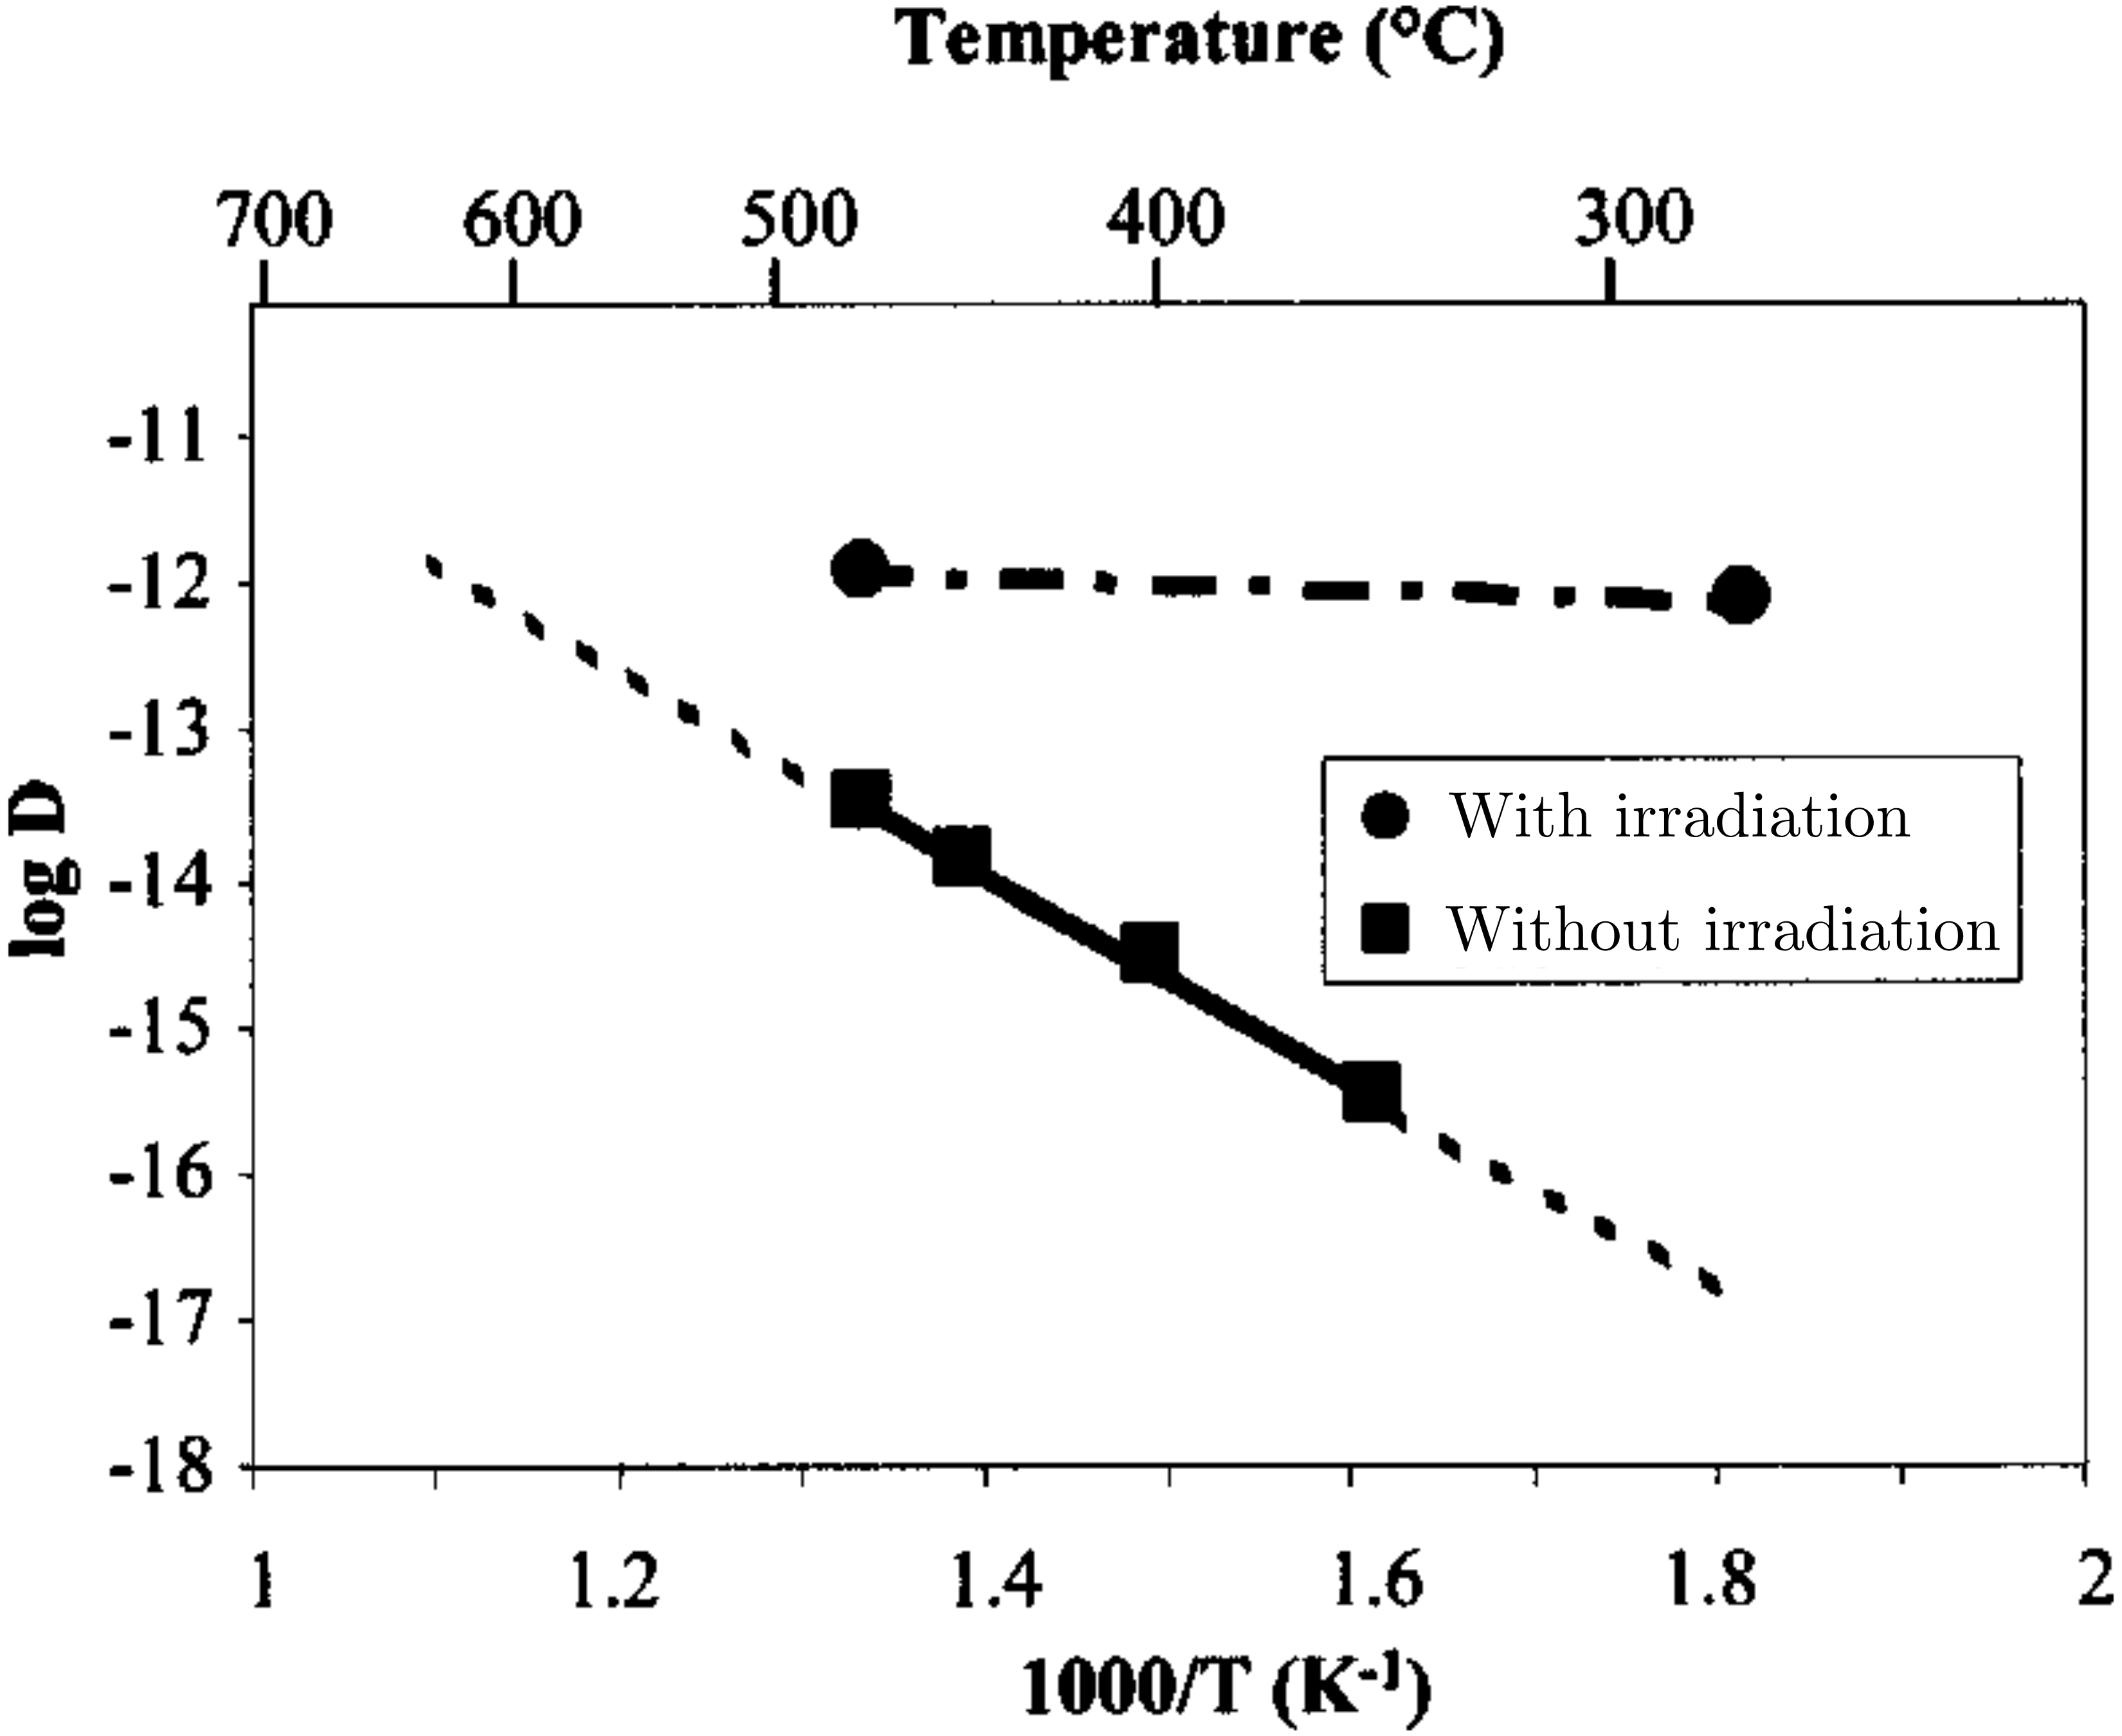
\includegraphics[width=0.65\textwidth]{Bererd_2005-Fig11-redraw.png}
        \caption[Courbe d'Arrhenius du coefficient de diffusion de l'oxygène dans la zircone.]{Courbe d'Arrhenius du
        coefficient de diffusion de l'oxygène dans la zircone \citep{Bererd2005}.}
        \label{fig:Bererd_diffusion_increase}
    \end{figure}


    L'irradiation par des rayonnements $\gamma$ peut augmenter de quelques ordres de grandeur la conductivité
    électronique de
    céramiques considérées isolantes telle que l'alumine \citep{Shikama1994}. \citet{Howlader1999} se sont intéressés à la
    conductivité de la zircone sous irradiation d'électrons de 1~MeV. L'auteur note une forte augmentation de
    la conductivité comme illustré sur la figure \ref{fig:conductivty_electron_beam}, et que l'impact de
    l'irradiation d'électrons diffère selon la nuance considérée. 


    \begin{figure}[H]
        \centering
        \begin{subfigure}[b]{0.48\textwidth}
            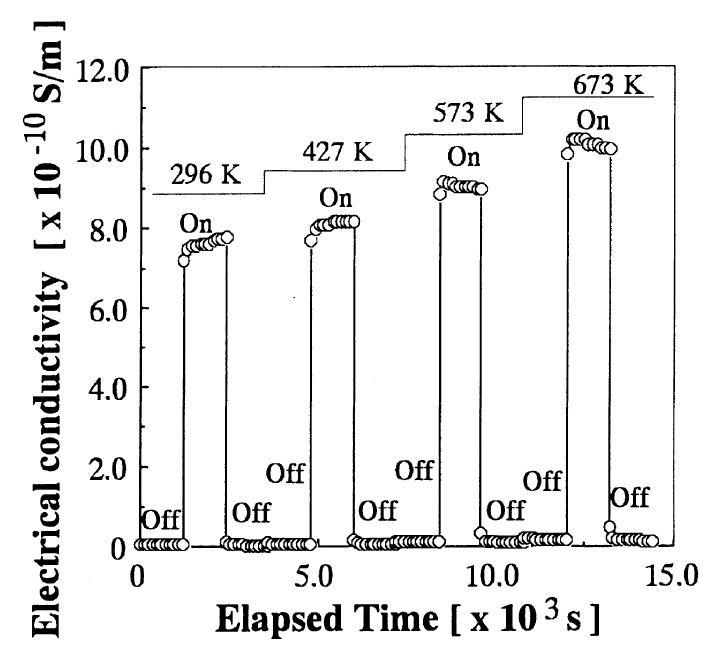
\includegraphics[width=\textwidth]{Howlader_1999-Fig6a.png}
            \caption{}
            \label{subfig:conductivity_gamma_Zy2}
        \end{subfigure}
        \quad
        \begin{subfigure}[b]{0.48\textwidth}
            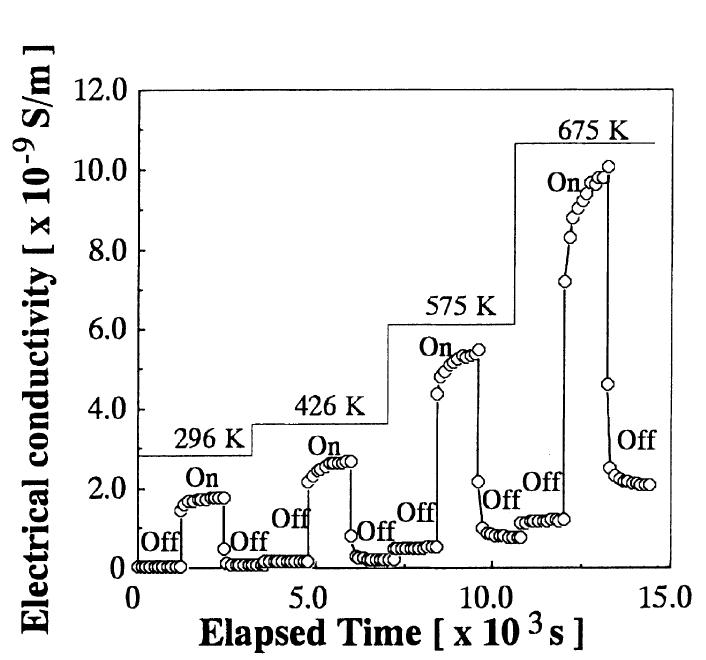
\includegraphics[width=\textwidth]{Howlader_1999-Fig6b.png}
            \caption{}
            \label{subfig:conductivity_gamma_improved_Zy2}
        \end{subfigure}
        \quad
        \begin{subfigure}[b]{0.48\textwidth}
            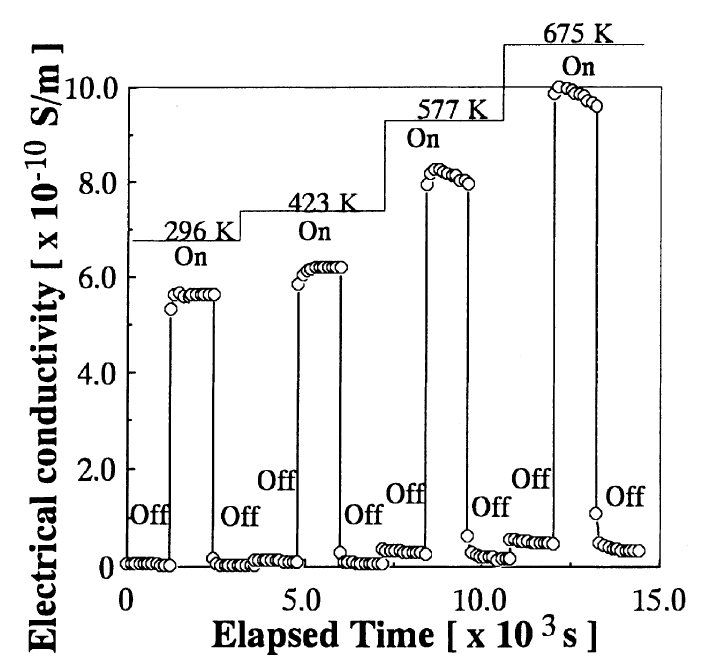
\includegraphics[width=\textwidth]{Howlader_1999-Fig6c.png}
            \caption{}
            \label{subfig:conductivity_gamma_Zy4}
        \end{subfigure}
    \caption[Effet de l'irradiation avec des électrons (1 MeV avec un flux de \num{1.4e18}~$e m^{-2} s^{-1}$) sur la conductivité électronique
    de la couche de zircone sur l'alliage: a) Zircaloy-2, b) Zircaloy-2 modifié et c) Zircaloy-4.]
    {Effet de l'irradiation avec des électrons (1 MeV avec un flux de \num{1.4e18}~$e m^{-2} s^{-1}$) sur la conductivité électronique
    de la couche de zircone sur l'alliage: a) Zircaloy-2, b) Zircaloy-2 modifié et c) Zircaloy-4 \citep{Howlader1999}.}
    \label{fig:conductivty_electron_beam}
    \end{figure} 
    
    Le rayonnement neutronique ainsi que le rayonnement $\gamma$ sont également responsables de la radiolyse de l'eau
    \citep{Cowan2011}. Les réactions chimiques pouvant se produire entre les différents produits de radiolyse sont
    nombreuses \citep{Trupin-Wasselin2000, Auclair2001}. Parmi les produits de radiolyse primaire, c'est-à-dire ceux
    qui ont une durée de vie assez longue pour réagir chimiquement (de quelques nanosecondes à la milliseconde \citep{Trupin-Wasselin2000}), on trouve les espèces $e^-_{aq}$, $HO^{\bullet}$,
    $H^{\bullet} $,  $HO_2^{\bullet}$ et $H_2O_2$. Le peroxyde d’hydrogène possède la plus longue durée de vie et
    reste par conséquent le produit majoritaire de la radiolyse de l'eau. Néanmoins, sa concentration n'est pas
    identique sur toute la longueur de la gaine comme illustré sur la figure \ref{fig:radiloytic_species_profil} et les
    concentrations locales peuvent différer des valeurs en volume notamment au niveau des grilles de maintien. A cette 
    hétérogénéité de concentration de peroxyde d'hydrogène correspond une hétérogénéité de pouvoir oxydant de
    l'environnement le long de la gaine.  

    \begin{figure}[H]
        \centering
        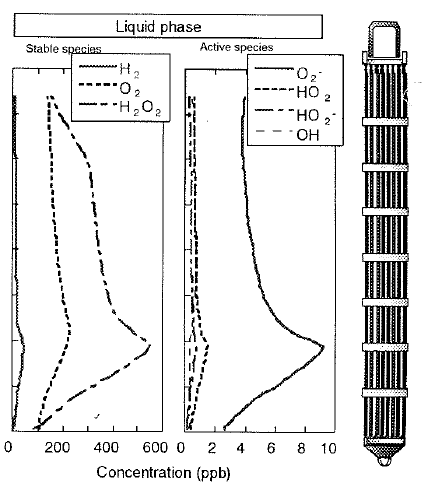
\includegraphics[width=0.75\textwidth]{Adamson_2002_Fig1-3-H2O2.png}
        \caption[Profil de concentration calculé des produits de radiolyse le long des gaines.]
        {Profil de concentration
        calculé des produits de radiolyse le long des gaines \citep{Adamson2002}.}
        \label{fig:radiloytic_species_profil}
    \end{figure}

    
    Il a été proposé que la présence de peroxyde d'hydrogène peut engendrer une dissolution locale de la couche de zircone
    \citep{IAEA1997}. \citet{Nishino1997} montrent que de la zircone massive stabilisée à l'yttrium est susceptible d'être
    dissoute lorsque cette dernière est irradiée par un rayonnement $\gamma$ à \SI{25}{\degreeCelsius} comme illustré
    par la figure \ref{subfig:Nishino_gamma_effect_YSZ}. La figure \ref{subfig:Nishino_gamma_effect_Zy2}, qui montre
    les prises de masse mesurées sur un alliage de Zircaloy-2 sous irradiation $\gamma$ à
    \SI{288}{\degreeCelsius}, semble confirmer cette observation.

    \begin{figure}[H]
        \centering
        \begin{subfigure}[b]{0.42\textwidth}
            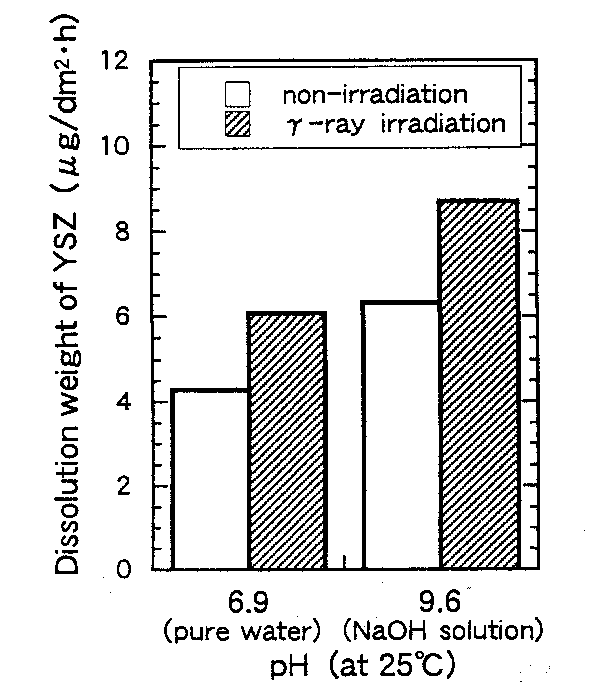
\includegraphics[width=\textwidth]{Nishino_1997-Fig8.png}
            \caption{}
            \label{subfig:Nishino_gamma_effect_YSZ}
        \end{subfigure}
        \quad
        \begin{subfigure}[b]{0.48\textwidth}
            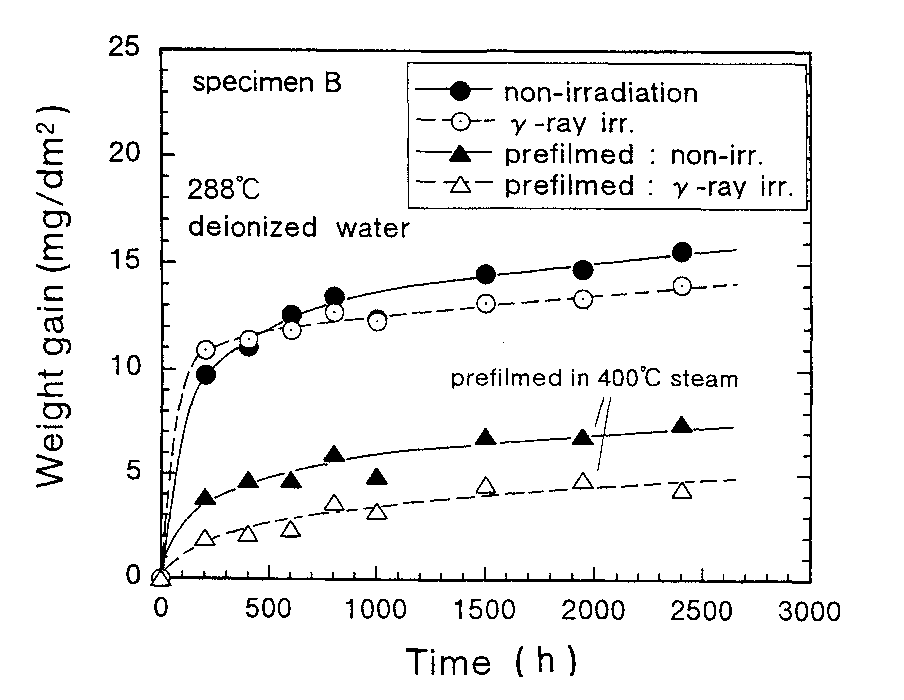
\includegraphics[width=\textwidth]{Nishino_1997-Fig3.png}
            \caption{}
            \label{subfig:Nishino_gamma_effect_Zy2}
        \end{subfigure}
        \caption[Effet de l'irradiation $\gamma$: 
        a) perte de masse de la zircone stabilisée à l'yttrium dans l'eau à \SI{25}{\degreeCelsius} sous irradiation,
        b) prise de masse de alliage Zircaloy-2  dans de l'eau pure à \SI{288}{\degreeCelsius} sous irradiation
    $\gamma$.]
        {Effet de l'irradiation $\gamma$: 
        a) perte de masse de la zircone massive stabilisée à l'yttrium dans l'eau à \SI{25}{\degreeCelsius} sous irradiation,
        b) prise de masse de alliage Zircaloy-2  dans de l'eau pure à \SI{288}{\degreeCelsius} sous irradiation $\gamma$
        \citep{Nishino1997}.}
        \label{fig:Nishino_Gamma_Effect}
    \end{figure}

    
    Par ailleurs, \citet{Cox1989} se sont intéressés à l'impact de l'illumination UV avec une lampe Xe 150W sur l'oxydation
    de l'alliage Zircaloy-2 à température ambiante.
    Ces auteurs montrent que l'illumination UV peut engendrer une légère augmentation de
    l'épaisseur de la couche de zircone sous une forte polarisation anodique. 
    %Cependant, l'utilisation de solution très
    %acide ou très basique ne permet pas de conclure si l'augmentation d'épaisseur serait également observée à pH neutre. 
    %Plus récemment, \citet{Goossens1996} ont étudié l'impact de la lumière UV sur une couche de zircone formée
    %anodiquement sur du zirconium
    %pure avec un potentiel imposé de \SI{12}{\volt}. La longueur d'onde de la lumière UV utilisée était de
    %\SI{220}{\nano\meter} avec une puissance de \SI{452}{\micro\watt\per\square\centi\meter}.
    %L'épaisseur de la couche de zircone a augmentée de \SI{1}{\nano\meter} pour une durée d'illumination d'environ
    %\SI{15}{\minute}. L'augmentation d'épaisseur a été attribuée à une diminution de l'intensité du champ électrique
    %dans la couche de zircone.

    L'étude de l'effet de l'irradiation n'est pas simple car elle peut agir simultanément sur le transport ionique et
    le transport électronique de la couche de zircone. Les effets sur le transport ionique et électronique peuvent être
    quantifiés sur les branches anodiques et cathodiques des courbes de polarisation, respectivement. 
    \citet{Cox1968} a proposé une synthèse des modifications hypothétiques subies par les branches anodiques et
    cathodiques sous irradiation en fonction de l'environnement comme illustré sur la figure
    \ref{fig:irradiation_effect_IE_plots}. Les courbes de polarisations anodiques et cathodiques classiquement mesurées en
    autoclave sur les alliages de zirconium sont présentées en figure \ref{fig:irradiation_effect_IE_plots}a).
    La présence de l'irradiation seule, illustrée par la figure \ref{fig:irradiation_effect_IE_plots}b), 
    impacterait seulement la branche anodique et induirait une faible augmentation du courant de corrosion, 
    alors que la présence supplémentaire d'oxygène, illustrée par la figure \ref{fig:irradiation_effect_IE_plots}c), impacte 
    les deux branches induisant ainsi une forte augmentation du courant de corrosion. La figure
    \ref{fig:irradiation_effect_IE_plots}d) illustre que la pré-oxydation permet de diminuer le courant de corrosion.

    En prenant en compte la possibilité d'avoir des branches anodiques et
    cathodiques qui différent à l'échelle locale par rapport à l'échelle de la gaine entière, différents types de corrosion
    sous irradiation peuvent être observés. En effet, trois types majeurs de corrosion ont été
    définis: \emph{corrosion uniforme}, \emph{corrosion nodulaire} et la \emph{Shadow Corrosion}.

    \begin{figure}[H]
        \centering
        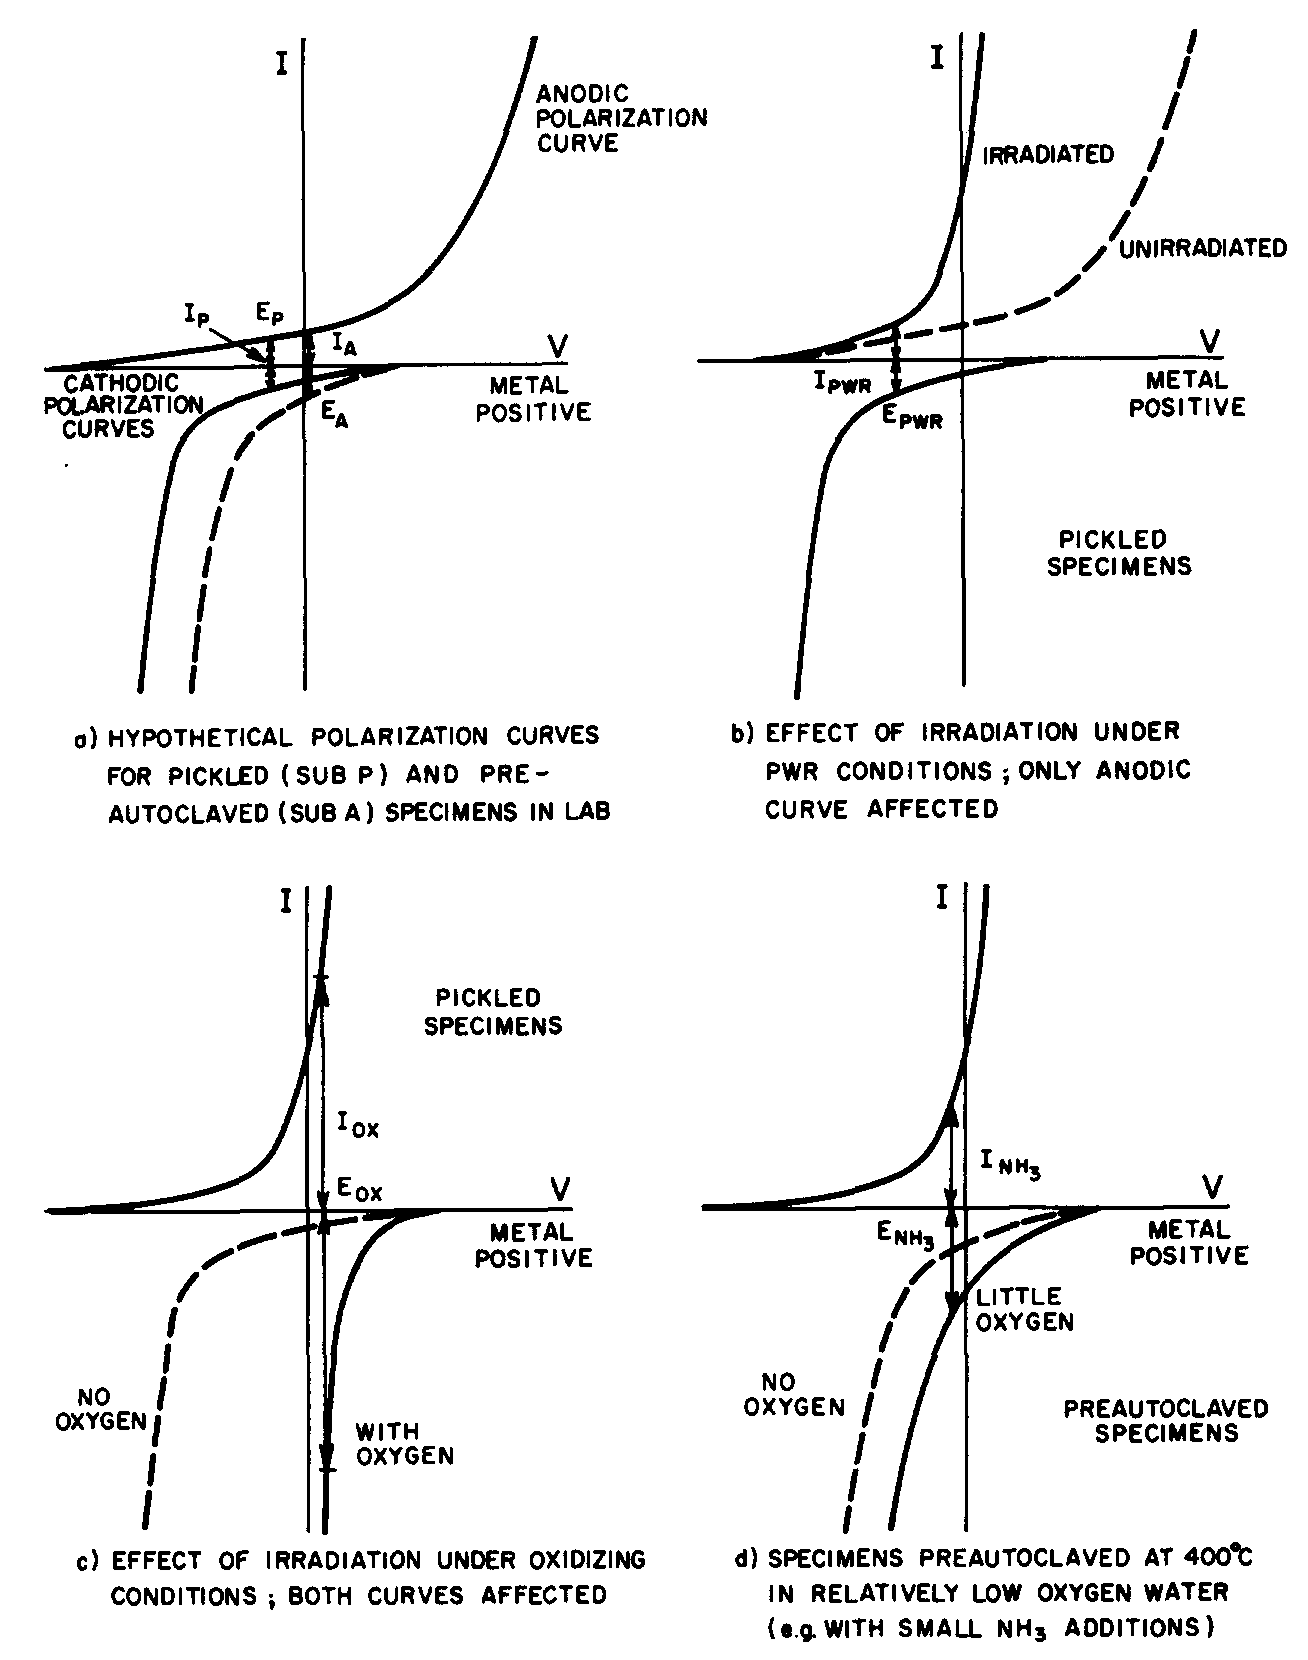
\includegraphics[width=0.9\textwidth]{Cox_1968b-Fig32.png}
        \caption[Effets hypothétiques de l'irradiation sur le transport ionique et électronique.]
        {Effets hypothétiques de
    l'irradiation sur le transport ionique (branche anodique) et électronique
        (branche cathodique) \citep{Cox1968-1}.}
        \label{fig:irradiation_effect_IE_plots}
    \end{figure}
    

    
    \subsection{Points clés de l'oxydation des alliages de zirconium}
        
        Moyennant quelques approximations, les mesures expérimentales de cinétique de prise de masse peuvent être
        converties en épaisseur de couche de zircone équivalente et en densité de courant d'oxydation équivalente. 

        La cinétique d'oxydation du Zircaloy-2 est relativement lente en autoclave. En effet, après un an d'oxydation en
        autoclave, la couche de zircone présente une épaisseur de seulement quelques microns. Cela correspond à une
        densité de courant entre 2 et 5 \si{\micro\ampere\per\square\centi\meter} au début de l'oxydation et elle
        atteint environ \SI{0.05}{\micro\ampere\per\square\centi\meter} après un an d'oxydation.

        La cinétique d'oxydation comporte deux régimes distincts (dits \emph{pré-transition} et \emph{post-transition}) séparés par
        une phase de \emph{transition}. La couche de zircone formée lors du 
        régime de pré-transition est plus dense alors que la couche formée lors du régime de post-transition 
        \citep{IAEA1998}. Généralement, la phase de \emph{transition} débute lorsque la couche de zircone atteint
        environ \SI{2}{\micro\meter}. Le profil cinétique d'oxydation du régime de
        \emph{pré-transition} est sub-parabolique alors qu'il est linéaire dans le régime de \emph{post-transition}.

        Les conditions oxydantes lors de la formation de la couche de zircone sont susceptible d'impacter sa
        conductivité en favorisant plus ou moins la dissolution d'éléments plus nobles tels que Fe, Cr et Ni
        pouvant doper la couche de zircone. En effet, la ségrégation de Fe et
        de Ni aux joints de grain de la couche de zircone peuvent favoriser le transport électronique.

        L'accélération de la cinétique d'oxydation ne dépend pas seulement de la conductivité électronique mais
        également de la conductivité ionique car les deux processus sont en équilibre. Dans le cas où les deux processus
        n'évoluent pas à la même vitesse dans les
        premiers instants de l'oxydation, une différence de potentiel apparaît entre l'interface interne et l'interface
        externe. Cette dernière accélère le processus le plus lent et ralentit le plus rapide.
        
        L’irradiation que subissent les matériaux englobe des rayonnements électromagnétiques allant des UV profonds aux
        rayonnements $\gamma$ ainsi que le rayonnement neutronique. Ces rayonnements peuvent impacter le transport ionique
        ainsi que le transport électronique des oxydes formés sur les gaines de confinement et les grilles de maintien. 
        La principale conséquence de l'irradiation est la perturbation de l'équilibre qui s'établit entre le transport
        ionique et le transport électronique afin d'assurer l'électroneutralité dans la couche de zircone. Toutefois, il
        semble y avoir peu de preuves avérées sur le lien direct entre l’accélération de la cinétique de corrosion et 
        l’augmentation des coefficients de diffusion de l’oxygène dans la couche de zircone.
        



%%%%%%%%%%%%%%%%%%%%%%%%%%%%%%%%%%%%%%%%%%%%%%%%%%%%%%%%%%%%%%%%%%%%%%%%%%%%%%%%%%%%%
%%%%%%%%%%%%%%%%%%%%%%%%%%%%%%%%%%%%%%%%%%%%%%%%%%%%%%%%%%%%%%%%%%%%%%%%%%%%%%%%%%%%%
\section{Phénomène de Shadow Corrosion}\label{sec:shadow_corrosion}

La Shadow Corrosion est communément définie comme un phénomène localisé de corrosion aggravée des alliages de zirconium
lorsque ces derniers se trouvent à proximité d'alliages plus \emph{nobles} tels que les alliages de nickel ou les aciers
inoxydables \citep{Chen1994}. Ce phénomène est uniquement observé dans les REB, dont
l'environnement est plus oxydant que dans les REP en raison de teneurs plus élevées
en oxygène et peroxyde d'hydrogène dissous dans l'eau \citep{Adamson2002}.

Pour mémoire, les assemblages de combustibles des REB sont constitués de gaines en alliage de zirconium de type Zircaloy-2
lesquelles sont maintenues par des grilles de maintien faites en alliage base nickel \cite{Garzarolli2011} comme
illustré sur la figure \ref{fig:what_is_shadow_corrosion}a. L'accroissement accéléré de la couche de zircone sur la gaine se situe
dans la zone en vis-à-vis de la grille de maintien. La surépaisseur de la couche de zircone peut atteindre dix fois la
valeur attendue pour une durée d'exposition donnée. Elle se manifeste par un oxyde de couleur blanche qui reproduit
la forme de la pièce en vis-à-vis comme on peut s'en rendre compte sur la figure \ref{fig:what_is_shadow_corrosion}b
\citep{Bischoff2012}.
Les grilles de maintien maintiennent les gaines de confinement à l'aide de ressorts qui sont en contact avec la surface
de ces dernière.
Une représentation schématique de la zone de contact est présentée en figure \ref{fig:what_is_shadow_corrosion}c.
 


    \begin{figure}[H] 
        \centering 
        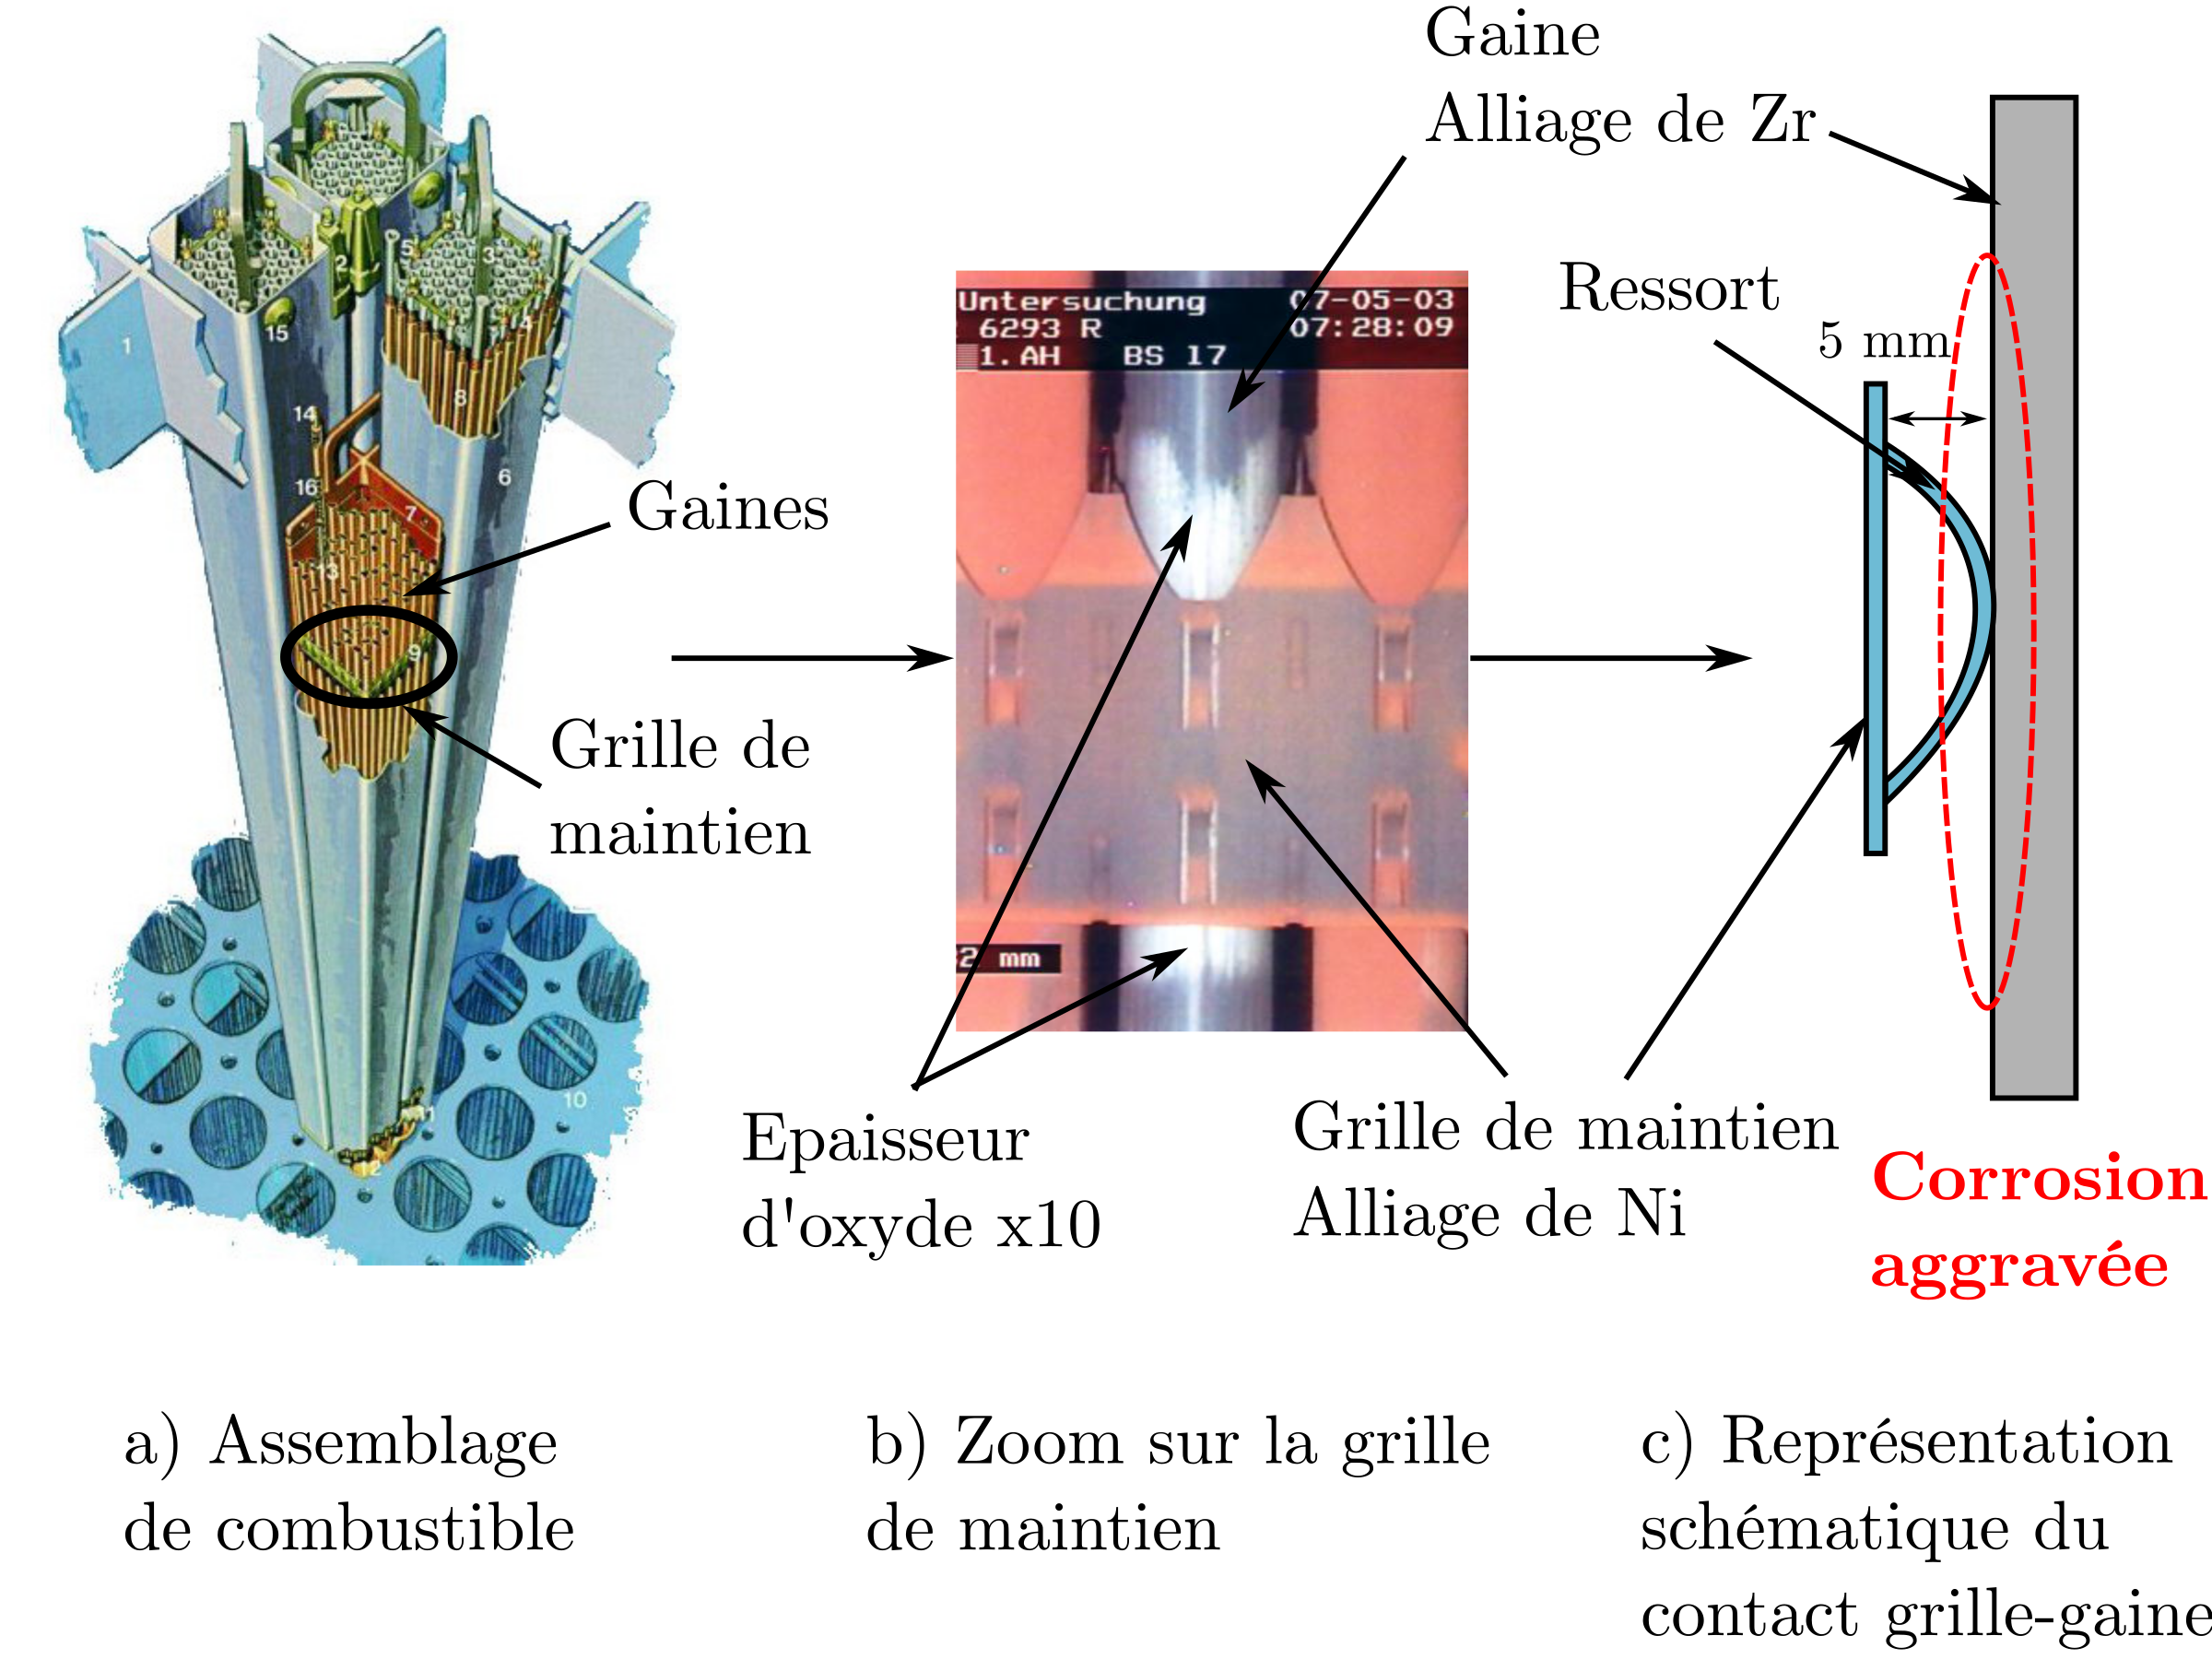
\includegraphics[width=0.95\textwidth]{what_is_shadow_corrosion.png}
        \caption[Schéma du phénomène de Shadow Corrosion]{Représentation schématique de la localisation du phénomène de
     Shadow Corrosion sur les assemblages de combustible dans un REB.} 
        \label{fig:what_is_shadow_corrosion} 
     \end{figure}


Le phénomène de Shadow Corrosion est connu depuis les années 1970. \citet{Johnson1974} ont signalé l’apparition de
corrosion accélérée sur des coupons de zirconium à proximité de pièces en platine dans un réacteur test.
\citet{Trowse1977} ont également observé la présence de corrosion aggravée des gaines de confinement sous les grilles
de maintien dans un réacteur à eau lourde. Cependant, ce phénomène n'a été étudié qu'à partir des années 2000 lorsqu’une
rupture de gaine de confinement s'est produite dans un REB en Suisse (réacteur KKL, Westinghouse, 
figure \ref{fig:fuel_rod_failure_KKL}).
Le mécanisme de rupture a été attribué à une forme aggravée de
Shadow Corrosion au niveau des grilles de maintien \citep{Edsinger2004}, dénommée par la suite ESCC
(Enhanced Spacer Shadow Corrosion).
Le problème a été partiellement résolu en s'appuyant sur les données de fonctionnement du réacteur antérieures à
l'incident, dont l'analyse a conduit au réajustement du ratio de $\frac{[Fe_{aq}]}{[Ni_{aq}]+[Zn_{aq}]}$ 
dans l'eau afin qu'il soit supérieur à 2, à l'augmentation de la teneur en fer dans l'alliage 
de zirconium et au changement d'un paramètre de recuit de l'alliage de zirconium \citep{Edsinger2004}.

         
     \begin{figure}[H] 
        \centering 
        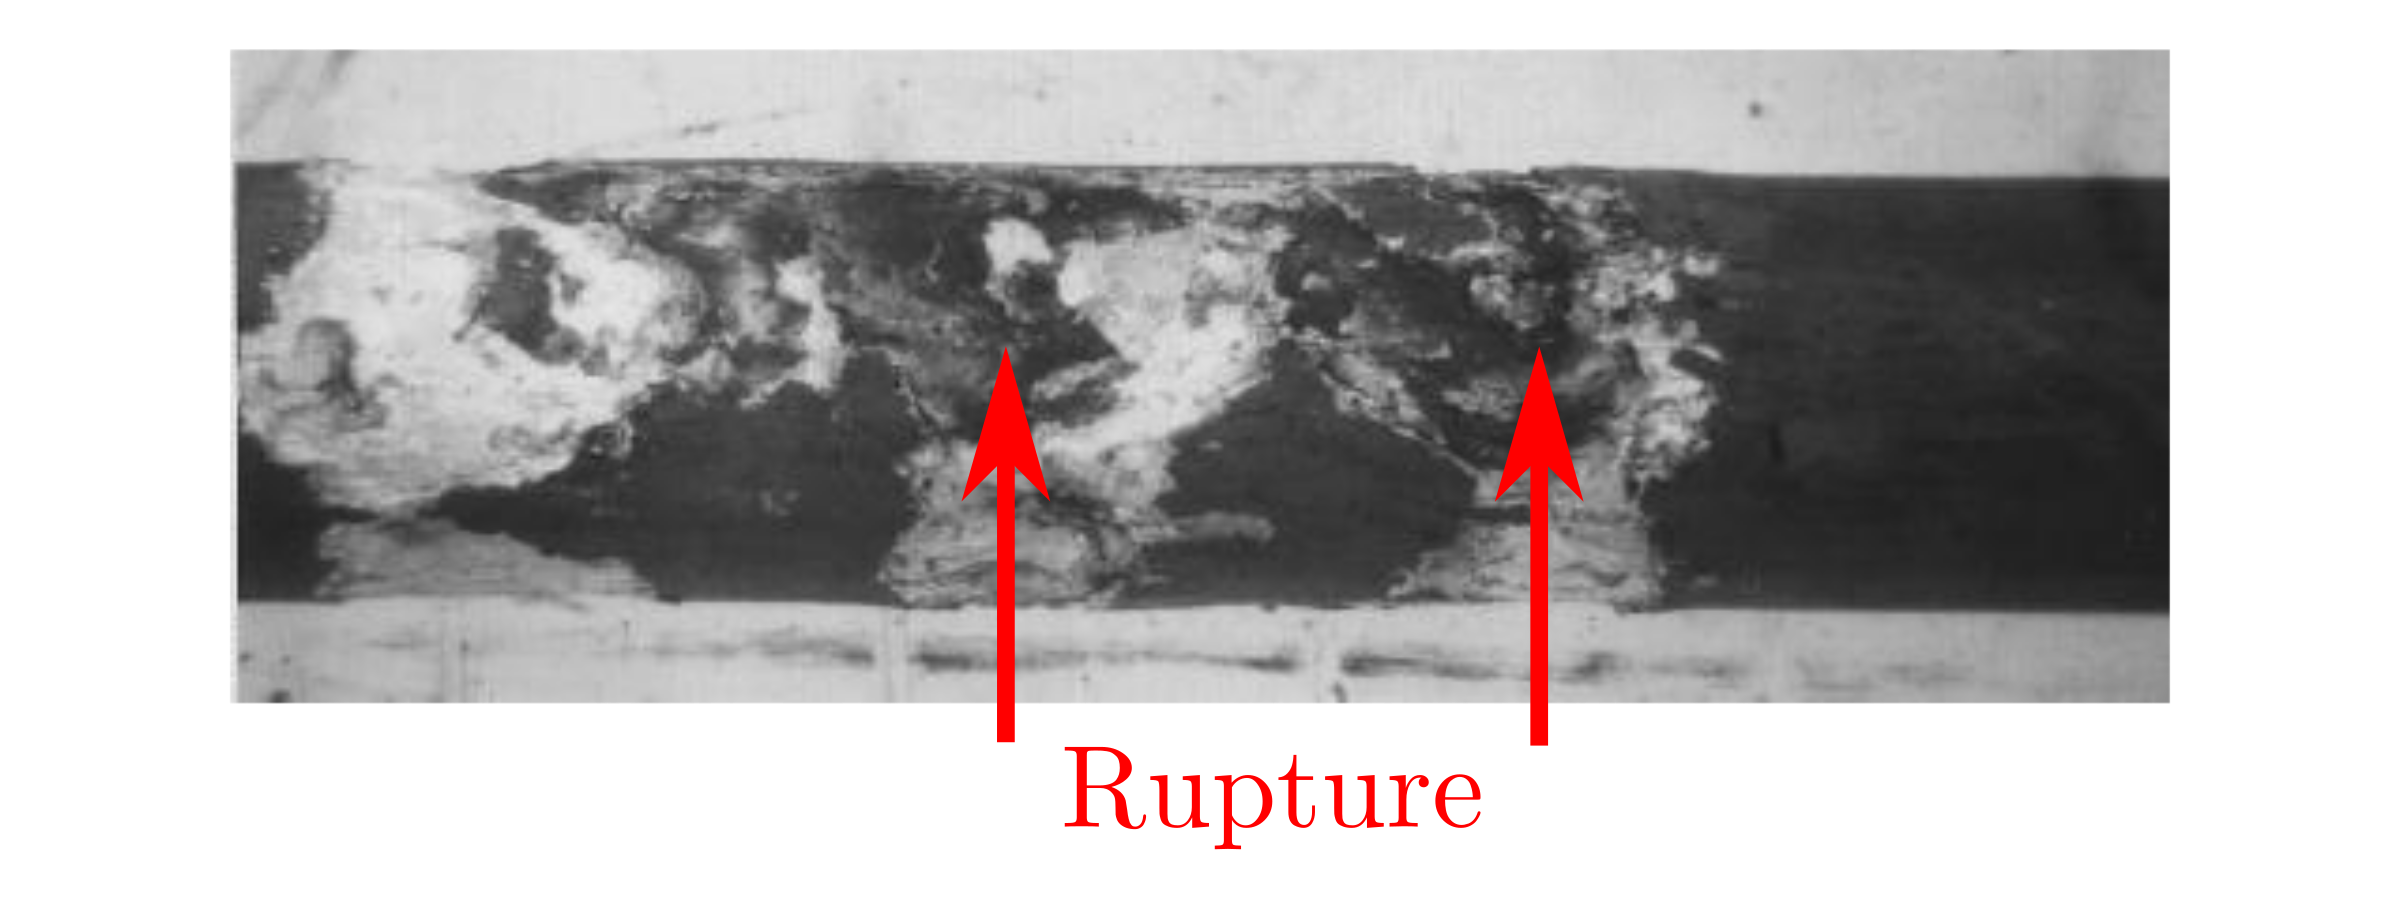
\includegraphics[width=0.6\textwidth]{rod_failure.png}
        \caption[Photographie illustrant la rupture d'une gaine de confinement dans le réacteur KKL]
        {Photographie illustrant la rupture d'une gaine de confinement dans le réacteur KKL \citep{Edsinger2004}.} 
        \label{fig:fuel_rod_failure_KKL} 
     \end{figure}


Des suivis de l'évolution de l'épaisseur de zircone sur les gaines sont effectués pendant la durée de mise en service de
ces dernières. Dans le cas de l'incident du réacteur KKL, les valeurs d'épaisseur de zircone ont été mesurées et celles-ci
ont été confrontées aux valeurs d'épaisseur de zircone obtenus lorsque le phénomène de Shadow Corrosion est absent comme
illustré sur la figure \ref{fig:KKL_shadow_values}. Il semble que le phénomène de Shadow Corrosion est apparu dès la
première année de mise en service avec une augmentation très rapide de l'épaisseur suivie par une période de
stabilisation. Une nouvelle augmentation forte de l'épaisseur de zircone, après trois ans de service, a mené à l'oxydation
totale de la gaine.

La figure \ref{fig:KKL_shadow_digitalization} a été obtenue à partir des données numérisées de la 
figure \ref{fig:KKL_shadow_values}, en calculant les densités de courant équivalentes à partir de l'équation
\ref{eq:th_to_j}. Il est clair que le peu de points disponibles rend cette estimation de la densité de courant très 
approximative. Cependant, elle permet de comparer les ordres de grandeur mis en jeu dans le cas
d'une cinétique d'oxydation classique et d'une cinétique d'oxydation de type Shadow Corrosion. 

    \begin{figure}[H] 
        \centering 
        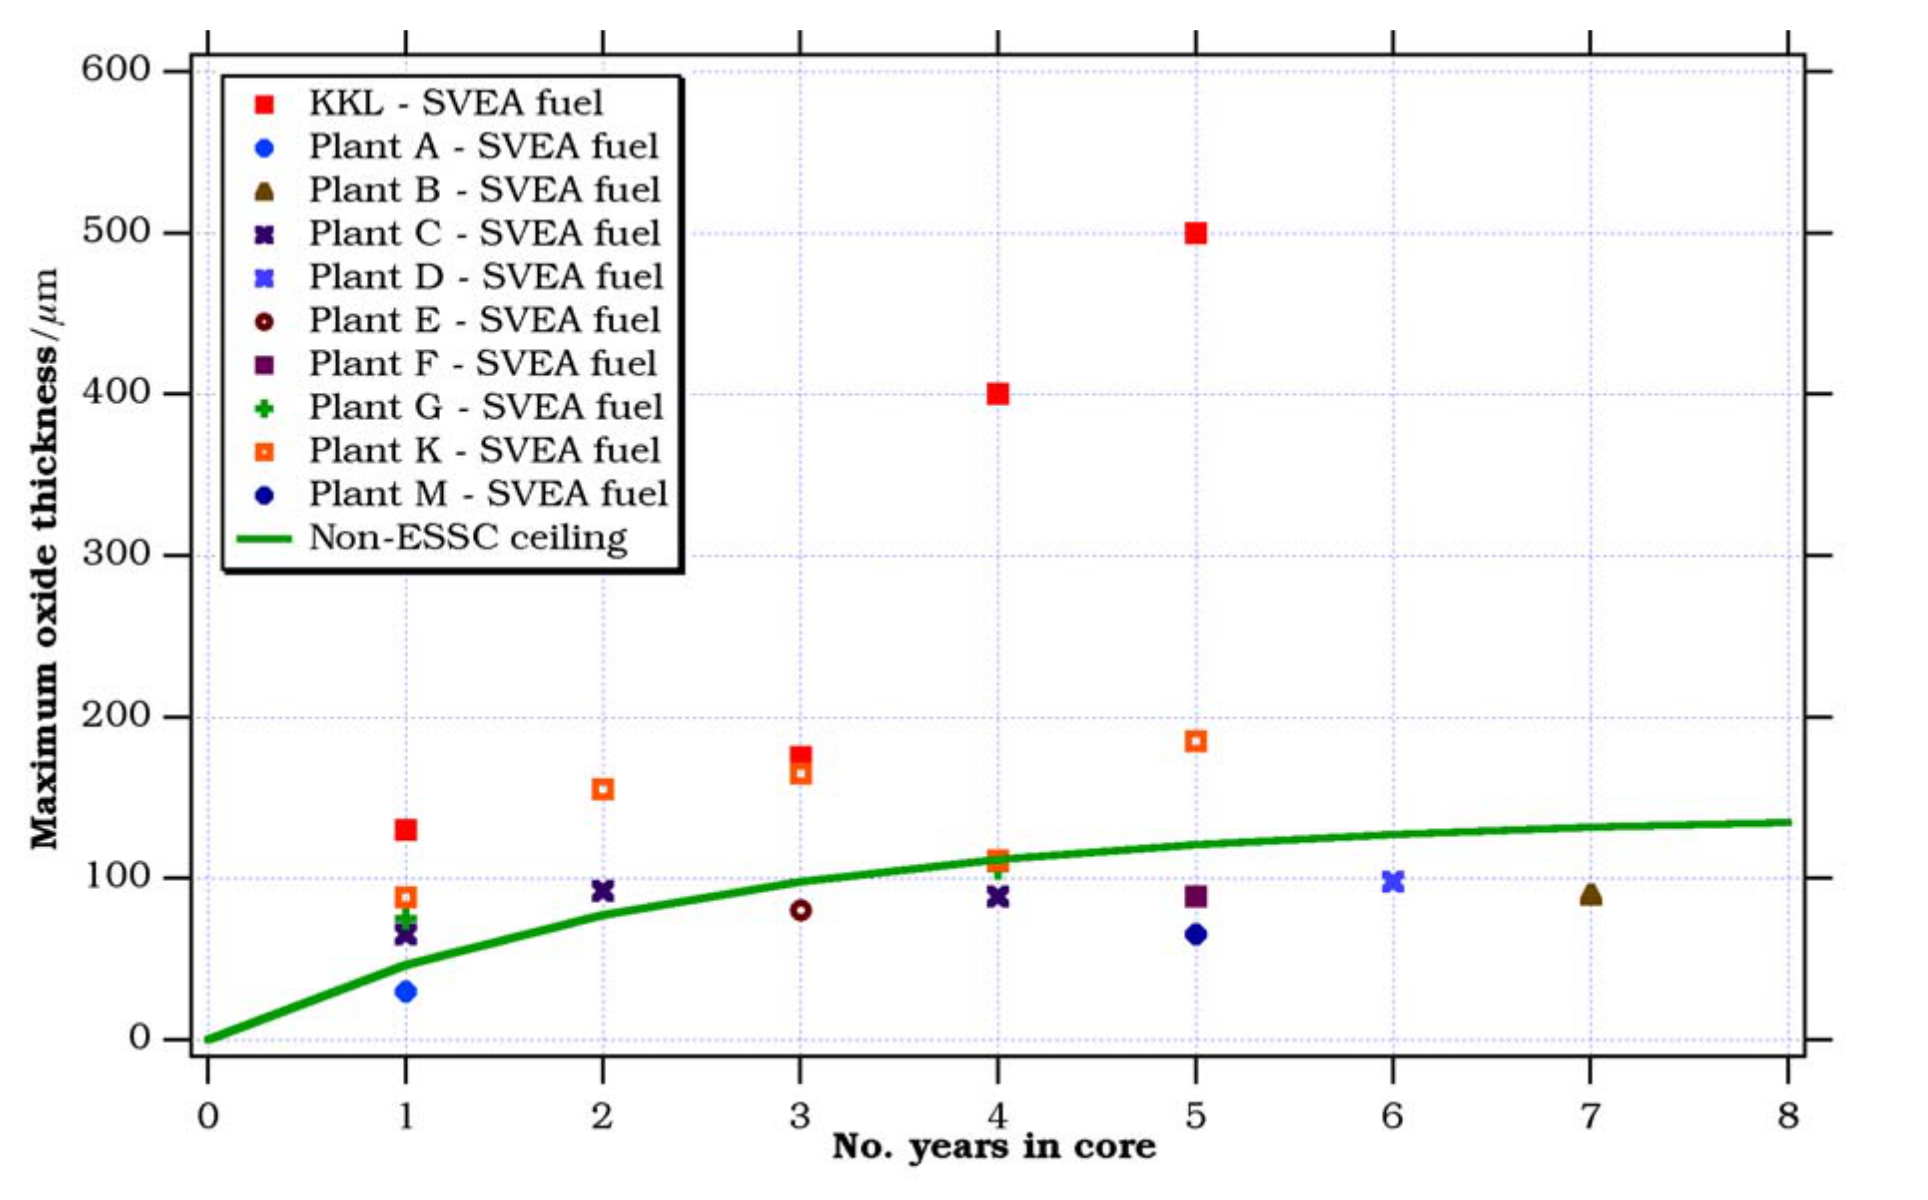
\includegraphics[width=0.65\textwidth]{Edsinger_2004-Fig_2_15.png}
        \caption[Evolution de l'épaisseur de la couche de zircone formée sur les gaines en fonction du temps d'exposition en réacteur
        dans le cas d'une corrosion classique et dans le cas de Shadow Corrosion.]
        {Evolution de l'épaisseur de zircone formée sur les gaines en fonction du temps d'exposition en réacteur
        dans le cas d'une corrosion classique et dans le cas de Shadow Corrosion \citep{Edsinger2004}.} 
        \label{fig:KKL_shadow_values} 
     \end{figure}  

     \begin{figure}[H]
         \centering
            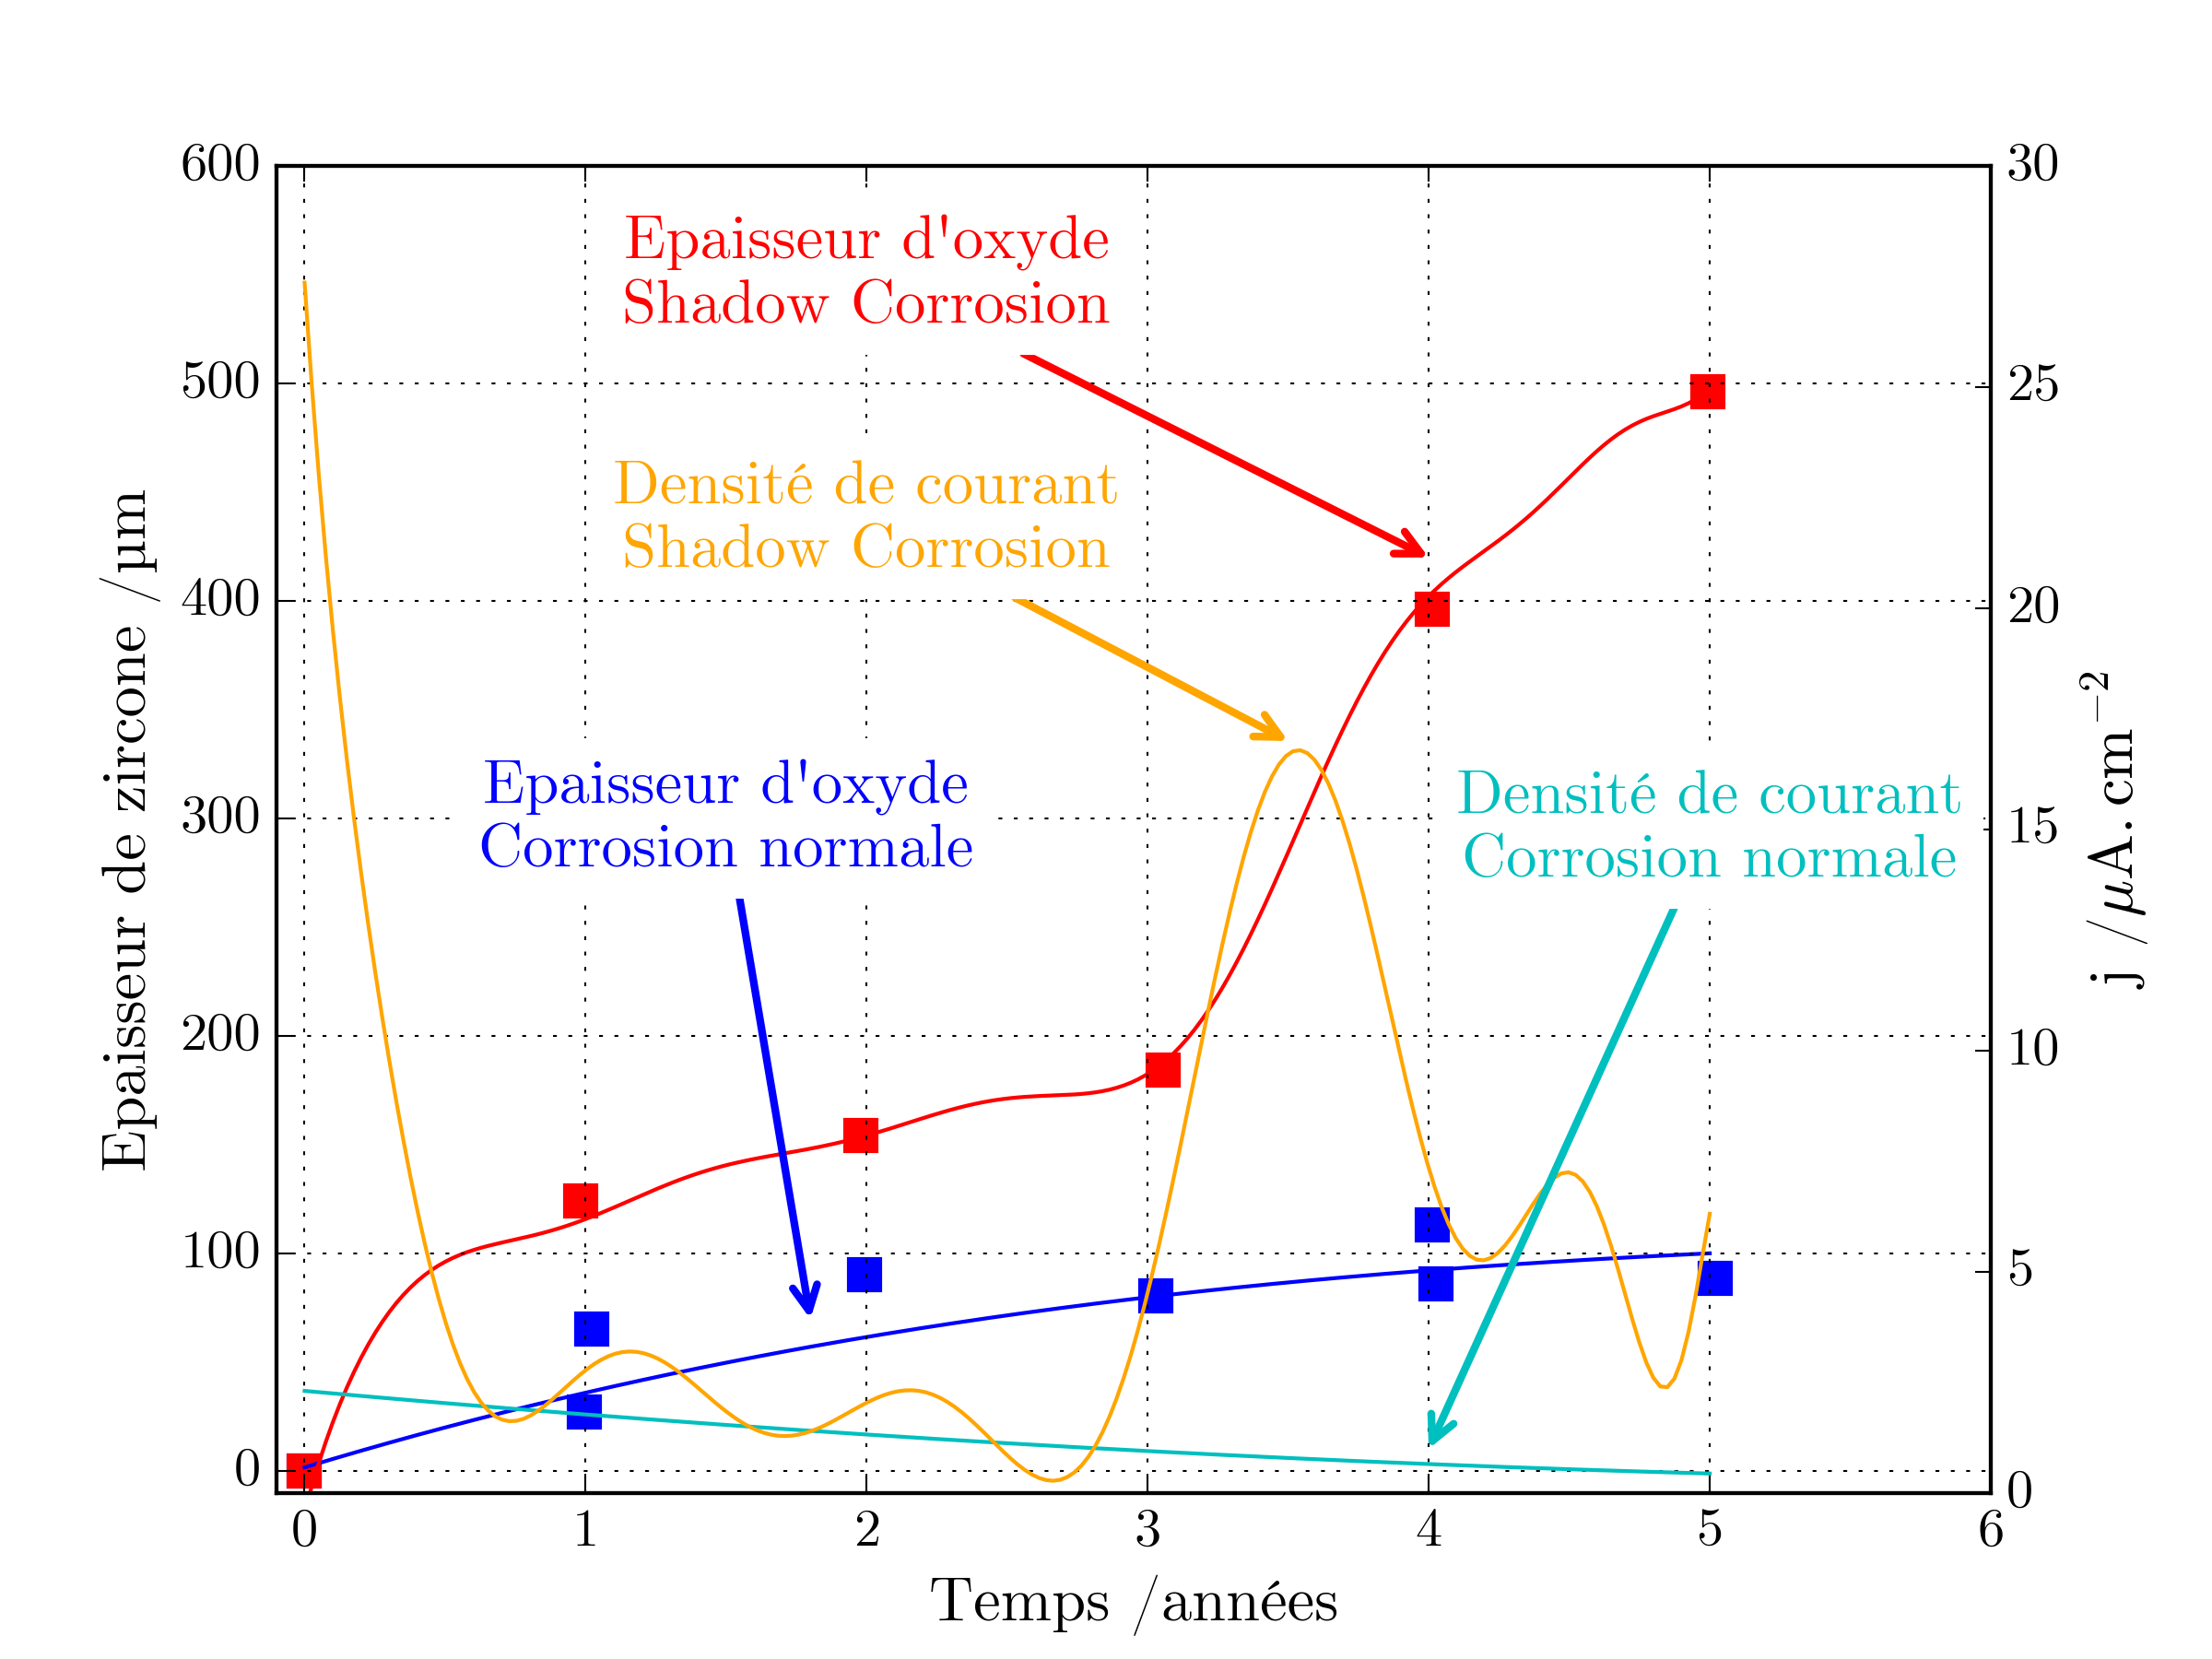
\includegraphics[width=0.65\textwidth]{Bischoff_2012_Fig2-Plot.png}
            \caption{Densité de courant équivalentes calculées selon l'équation \ref{eq:th_to_j} à partir des données
            numérisées de la figure \ref{fig:KKL_shadow_values}.} 
            \label{fig:KKL_shadow_digitalization} 
    \end{figure} 
    
Dans le cas d'une corrosion classique, la densité de courant diminue constamment à partir de valeurs initiales
 de quelques \si{\micro\ampere\per\square\centi\meter} 
jusqu'à des valeurs finales de quelques dizaines de \si{\nano\ampere\per\square\centi\meter}.
En Shadow Corrosion on mesure une densité de courant initiale de quelques dizaines de 
\si{\micro\ampere\per\square\centi\meter}. Pendant la période de stabilisation, celle-ci reprend à des valeurs proches
des valeurs observées dans le cas d'une corrosion classique.
Après trois ans de fonctionnement, la densité de courant augmente à nouveau pour atteindre des valeurs voisines de
\SI{10}{\micro\ampere\per\square\centi\meter}. Cette analyse, certes très approximative, permet à minima de constater que la
densité de courant liée à la Shadow Corrosion est environ dix fois plus élevée que dans le cas d'une corrosion classique.


%%%%%%%%%%%%%%%%%%%%%%%%%%%%%%%%%%%%%%%%%%%%%%%%%%%%%%%%%%%%%%%%%%%%%%%%%%%%%%%%%%%%%
%%%%%%%%%%%%%%%%%%%%%%%%%%%%%%%%%%%%%%%%%%%%%%%%%%%%%%%%%%%%%%%%%%%%%%%%%%%%%%%%%%%%%
\section{Etudes expérimentales de la Shadow Corrosion en réacteur test}\label{sec:in_pile_reactor}

    A la suite de l’incident du réacteur KKL, Westinghouse a lancé trois séries de
    tests expérimentaux dans des réacteurs de recherche afin
    d’étudier le phénomène de Shadow Corrosion. Ces réacteurs de recherche
    permettent de simuler les conditions de fonctionnement d’un REB
    en termes de pression, de température, de flux de neutron et de chimie de
    l’eau. Les résultats issus de ces expériences ont permis de lister les
    paramètres qui semblaient avoir un impact fort sur le phénomène de Shadow Corrosion.

    Les études expérimentales ont été menées dans trois réacteurs de recherche différents :
    le réacteur de Studsvik R2 en Suède \citep{Nystrand1999}, le réacteur MITR-II
    aux Etats-Unis \cite{Chatelain2000} et le réacteur de Halden en Norvège
    \cite{Andersson2002}. La principale donnée de sortie était l’épaisseur de la
    couche de zircone qui s’est formée sur la gaine en Zircaloy-2 mesurée par observation métallographique ou par mesure
    des courants de Foucault.

    \subsection{Essais effectués dans le réacteur de Studvik (Suède)}\label{subsec:studvik}

	\subsubsection{Conditions expérimentales des essais}
        L’objectif de ce premier test était de vérifier si le phénomène de Shadow
        Corrosion peut être observé sur des gaines de confinement en Zircaloy-2
        placés dans une grille de maintien en alliage de nickel X750 après une
        courte période d’exposition dans le coeur du réacteur test. Les gaines de
        Zircaloy-2, en contact avec les grilles de maintien, étaient placées en parallèle dans le
        coeur et hors du coeur du réacteur pendant 5 semaines avec une chimie
        déficiente en fer comme dans le cas de l’incident du réacteur KKL.
        Différents traitement de surface ont été testés sur les gaines de Zircaloy-2 dont  
        quatre ont été pré-oxydés jusqu'à une épaisseur de zircone de
        \SI{1}{\micro\meter} et deux jusqu'à une épaisseur de
        \SI{2}{\micro\meter}.
	
	\subsubsection{Résultats des essais}
        Le même phénomène que dans les réacteurs commerciaux a été observé
        c’est-à-dire que les échantillons placés dans le coeur du réacteur présentaient
        une couche de zircone de \SI{10}{\micro\meter} alors que les échantillons
        placés hors du coeur présentaient une couche de zircone de \SI{1}{\micro\meter}. L'augmentation d'épaisseur de la couche
        de zircone n'a été observée qu'au point de contact et aucune surépaisseur n'a été observée dans la zone autour
        du point de contact grille-gaine.
        Il n’y a pas d’effet notable du traitement de surface. 

        La présence d’irradiation
        semble donc être une condition nécessaire pour reproduire le
        phénomène de Shadow Corrosion. Cependant, l’absence de couplage entre la
        gaine et la grille est une condition expérimentale qui n'a pas été étudiée.


    \subsection{Essais effectués dans le réacteur du MIT (USA)}\label{subsec:MIT}

    \subsubsection{Conditions expérimentales des essais}
        L’objectif premier de ce test était d’étudier l’impact des matériaux de
        contre-électrode, c’est-à-dire les matériaux des grilles de maintien, sur le
        phénomène de la Shadow Corrosion. La durée de l'exposition était d'environ 7 semaines.
        Quatre matériaux ont été testés: l'alliage de
        nickel X750, le platine, l’alliage Nitronic 32 et l'alliage Zircaloy-2 qui est
        également le matériau de la gaine. L’alliage Nitronic 32 est alliage austénitique
        de fer contenant 12 \% en masse de manganèse qui est un émetteur de radiation $\beta$
        lorsqu’il est activé. Les échantillons étaient placés dans deux types de modules :
        module \emph{sans contact} et module \emph{avec contact}, représentés en figures
        \ref{fig:Modules_MIT_Test} et \ref{fig:Modules_MIT_Test_schematics}.

        \begin{figure}[H] 
            \centering 
            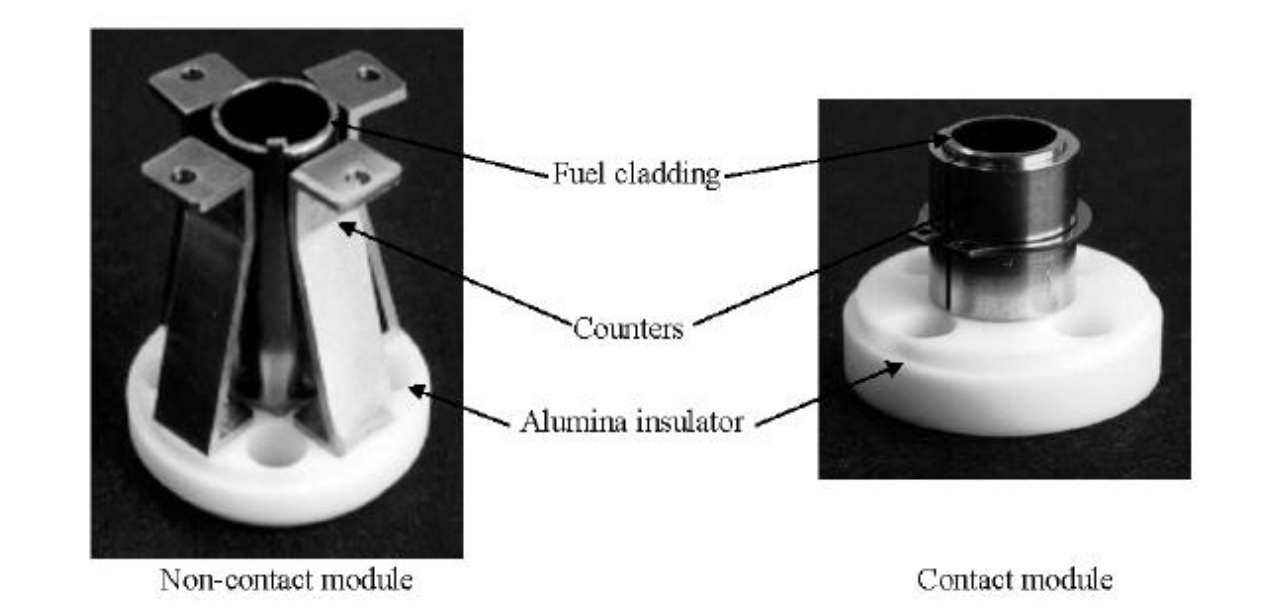
\includegraphics[width=0.65\textwidth]{Bischoff_2012_Fig8.png} 
            \caption[Photographies des modules testés dans le réacteur MITR-II.]
            {Photographies des modules testés dans le réacteur MITR-II \citep{Chatelain2000}.} 
            \label{fig:Modules_MIT_Test} 
        \end{figure}
        
        \begin{figure}[H] 
            \centering 
            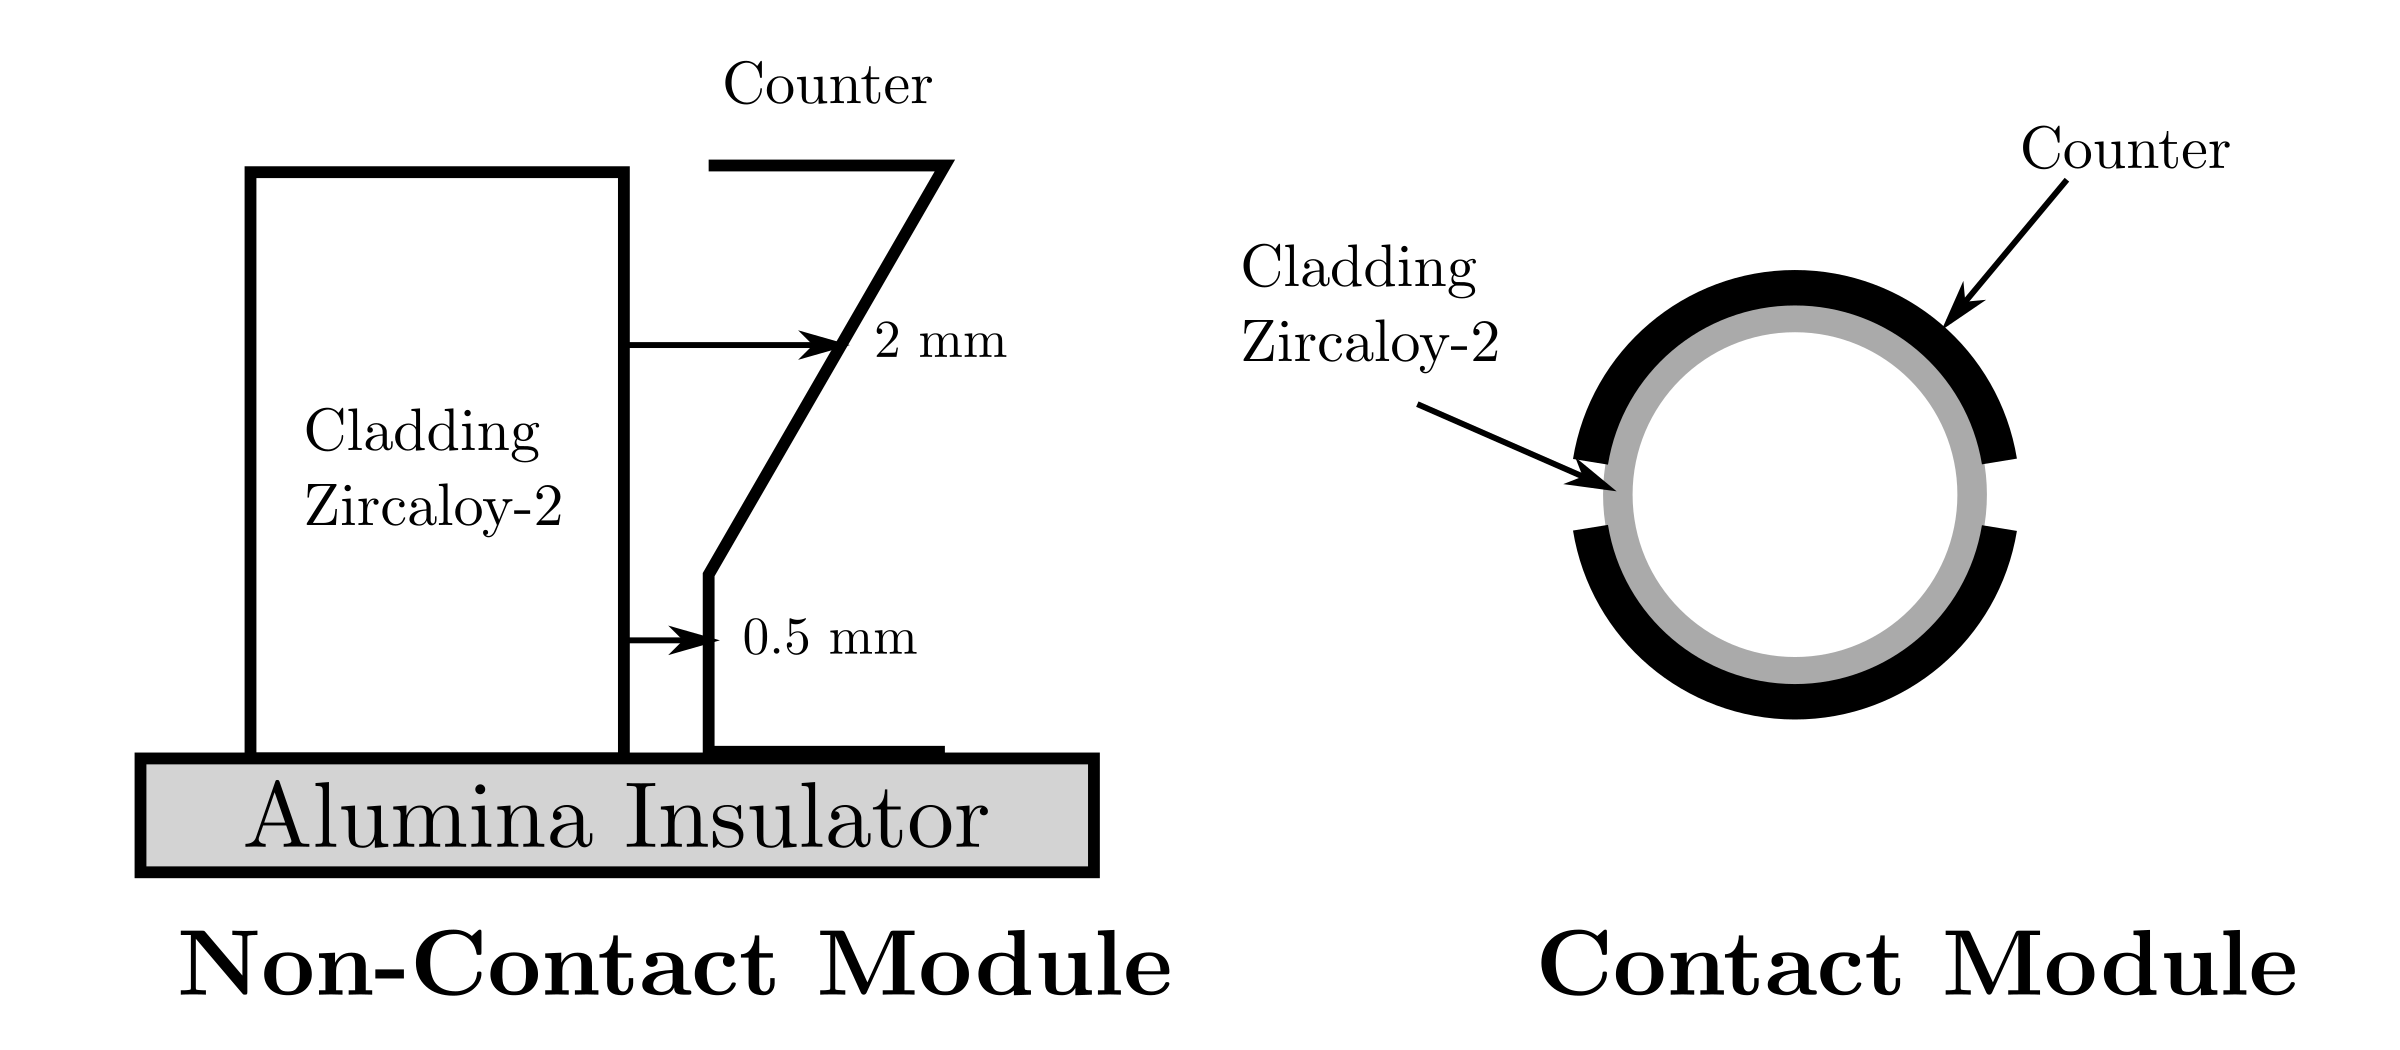
\includegraphics[width=0.65\textwidth]{Chatelain_2000-Modules-Both-Redrawn.png} 
            \caption[Représentation schématique des modules testés dans le réacteur MITR-II.]
            {Représentation schématique des modules testés dans le réacteur MITR-II \citep{Chatelain2000}.} 
            \label{fig:Modules_MIT_Test_schematics} 
        \end{figure}

        Les modules avec contact étaient constitués d’une gaine de Zircaloy-2 avec deux
        moitiés de tube en guise de contre-électrodes, ces dernières étant mises en contact
        avec la gaine et maintenues par un anneau en acier inoxydable. L’ensemble était
        placé sur un isolant en alumine. Les modules sans contact sont réalisés en
        isolant une gaine de Zircaloy-2 avec de l’alumine par rapport aux quatre contre-électrodes
        qui font face à la gaine. La forme des contre-électrodes permettait de
        contrôler leur distance (entre \SI{0.5}{\milli\meter} et \SI{2}{\milli\meter}) à la gaine en Zircaloy-2.

        La chimie d’un REB était reproduite dans le réacteur et le flux d’eau formait une boucle dans le
        réacteur comme illustré sur la figure \ref{fig:MITRII_reactor_schematics}. Des
        échantillons étaient placés dans le coeur, et hors du coeur du réacteur à environ
        \SI{60}{\milli\meter} en aval. Les échantillons ont été exposés pendant une période de 7 semaines, la dose
        de rayonnement gamma était environ deux ordres de grandeur inférieure hors du coeur
        par rapport au coeur alors que la dose de rayonnement neutronique était environ inférieure de cinq ordres de
        grandeurs.

	\begin{figure}[H] 
 		\centering 
 		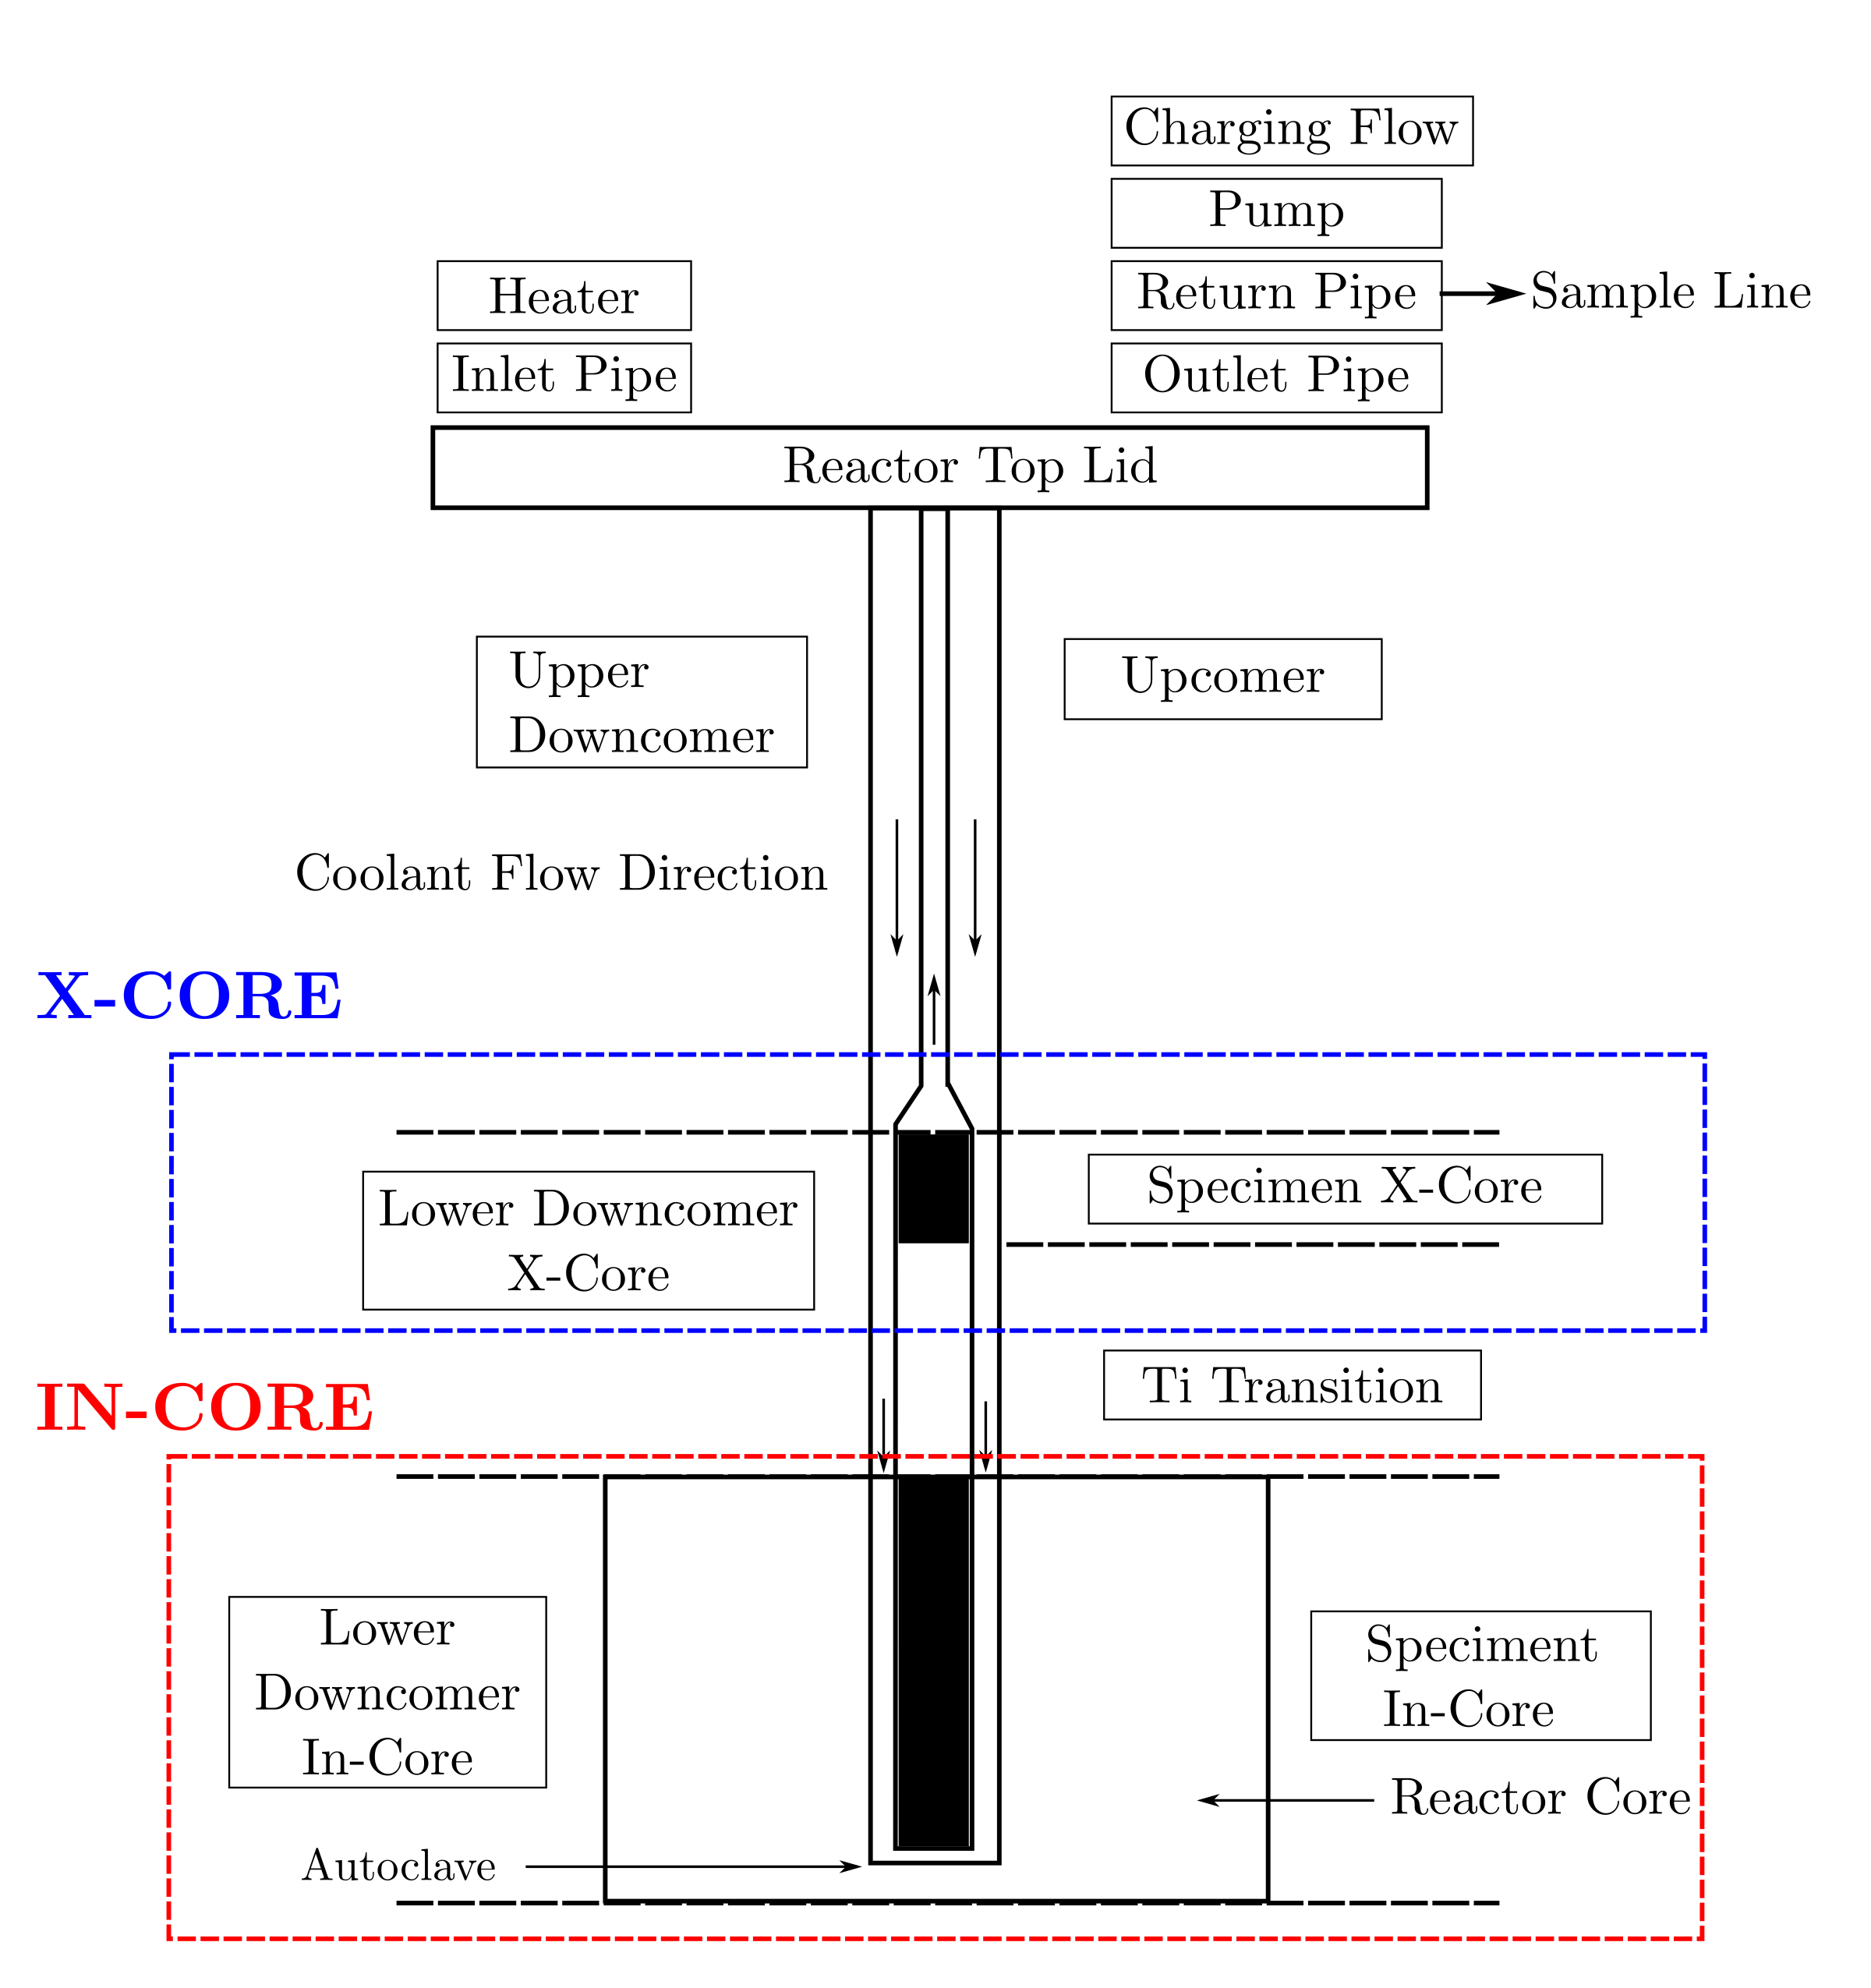
\includegraphics[width=\textwidth]{Chatelain_2000-InCore_ExCore_Locations-2.png} 
        \caption[Représentation schématique du réacteur test MITR-II.]
        {Représentation schématique du réacteur test MITR-II \citep{Chatelain2000}.} 
 		\label{fig:MITRII_reactor_schematics} 
 	\end{figure}
	
	\subsubsection{Résultats des essais}
        Dans le cas des modules sans contact, le phénomène de Shadow Corrosion n'a été
        observé qu'avec l’alliage de nickel X750 et le platine, quelles que
        soient les configurations expérimentales comme illustré en figure
        \ref{fig:oxide_thickness_vs_counter_material_non_contact_module}. Le
        phénomène de Shadow Corrosion apparaissant deux fois moins prononcé sur les
        échantillons hors du coeur. Par ailleurs, l’épaisseur de zircone était inversement
        proportionnelle à la distance entre la gaine et la contre-électrode
        (\ref{fig:oxide_thickness_vs_distance_non_contact_module}), l'ampleur du phénomène
        de Shadow Corrosion était rapidement atténué au-delà de
        \SI{1}{\milli\meter}. Il faut cependant souligner que l’alumine n’est pas un
        isolant parfait lorsqu'elle est irradiée \citep{Shikama1994} et
        que les modules dits sans contact ne peuvent donc probablement pas être réellement considérés en tant que
        tels.

        \begin{figure}[H]
            \centering
            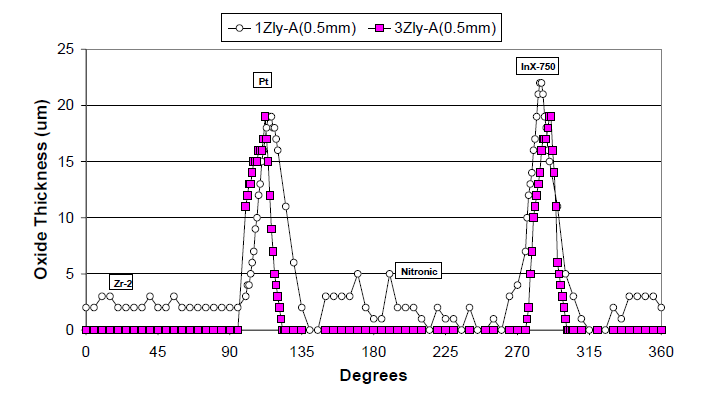
\includegraphics[width=0.65\textwidth]{Bischoff_2012_Fig9.png} 
            \caption[Epaisseurs de zircone mesurées sur le module sans contact en fonction des quatre types matériaux de
            contre-électrode pour une distance gaine--contre-électrode de \SI{0.5}{\milli\meter}.]
            {Epaisseurs de zircone mesurées sur le module sans contact en fonction des quatre types matériaux de
            contre-électrode pour une distance de \SI{0.5}{\milli\meter} \citep{Chatelain2000}.} 
            \label{fig:oxide_thickness_vs_counter_material_non_contact_module} 
        \end{figure}

        \begin{figure}[H] 
            \centering
            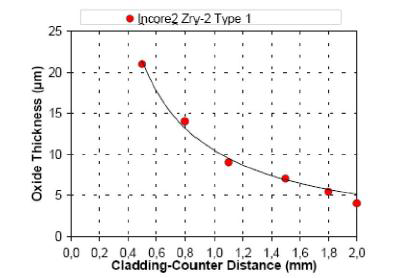
\includegraphics[width=0.65\textwidth]{Bischoff_2012_Fig10.png} 
            \caption[Epaisseurs de zircone mesurées en fonction de la distance pour le couple Zircaloy-2/X750.]
            {Epaisseurs de zircone mesurées en fonction de la distance gaine--contre-électrode pour le couple Zircaloy-2/X750 \citep{Chatelain2000}.}
            \label{fig:oxide_thickness_vs_distance_non_contact_module} 
        \end{figure}

        
        Sur les gaines des modules avec contact, il n a pas été observé de corrosion aggravée
        sur la surface située sous la contre-électrode. Cependant, une surépaisseur
        d’oxyde est apparue au voisinage de l’espacement entre les deux demi-tubes formant la
        contre-électrode, probablement en raison que l’électrolyte peut y accéder
        plus facilement à la surface de la gaine, favorisant ainsi le renouvellement
        de la chimie locale. Malgré une surface de contact élevée entre la gaine et les
        contre-électrodes, les modules avec contact présentent une surépaisseur
        d’oxyde plus faible que les modules sans contact quelle que soit leur position
        dans le réacteur. Tout comme pour les modules sans contact, seuls l’alliage de
        nickel X750 et le platine ont donné lieu au phénomène de Shadow Corrosion.
        
        Le phénomène de Shadow Corrosion apparaît donc avec des matériaux de
        contre-électrode plus nobles que l'alliage Zircaloy-2 tels que l’alliage de nickel X750 et le platine.
        La présence d'une irradiation et les doses de radiations sont des paramètres importants pour l'apparition de la
        Shadow Corrosion.
        La distance grille--gaine est
        également un paramètre important mais l’accès de l’électrolyte à la surface de
        la gaine et de la contre-électrode est tout aussi important. La circulation du
        fluide caloporteur, c’est-à-dire l’électrolyte, permet probablement de renouveler la
        chimie locale et ainsi de favoriser l'apparition de la Shadow Corrosion.

        
%        \citet{Treeman2005} a réalisée des essais supplémentaires dans ce même réacteur afin de quantifier les densités
%        de courants de couplage mis en jeu lorsque l'alliage Zircaloy-2 est en contact avec du Pt ou l'alliage de nickel X750. 
%        L'étude a été mené sur environ 50 jours avec des phases d'interruption. La figure \ref{fig:treeman_jgal}
%        présente les résultats obtenus retracé en fonction de la durée d'exposition afin de mieux visualiser les phases
%        à haute température ainsi que les phases à forte dose d'irradiation. 

%        Les résultats obtenus sont intéressants puisqu'ils mettent en avant l'importance de la température. A 20
%        d'exposition, la puissance du coeur est au maximum alors la température est à environ \SI{60}{\degreeCelsius}.
%        La densité de courant de couplage se situe à \SI{\sim 0.5}{\micro\ampere\per\square\centi\meter}. En maintenant,
%        la puissance constante et en augmentant la température à \SI{250}{\degreeCelsius}, la densité de courant de
%        couplage augmente brutalement jusqu'à \SI{\sim 10}{\micro\ampere\per\square\centi\meter}. Ce résultat
%        expérimental confirme bien le lien entre le transport ionique et le transport électronique.

%        \begin{figure}[!htb]
%            \centering
%            \includegraphics[width=0.45\textwidth]{Treeman_2005-Galvanic_Currents.pdf}
%            \caption[Résultats expérimentaux obtenus par Treeman et al. retracés en fonction du temps d'exposition.]
%            {Résultats expérimentaux obtenus par \citet{Treeman2005} retracés en fonction du temps d'exposition.
%            a) Evolution de la température. 
%            b) Evolution des courants de couplage. 
%            c) Evolution de la puissance du coeur.}
%        \end{figure}

        


    \subsection{Essais effectués dans le réacteur de Halden (Norvège)}\label{subsec:halden}

    \subsubsection{Conditions expérimentales des essais}
        Les objectifs de ce test était d'évaluer l’impact du flux
        neutronique, du flux de rayonnement gamma, des traitements thermiques, de la
        composition chimique des gaines de confinement et des matériaux de
        contre-électrode sur le phénomène de Shadow Corrosion dans le cas d'une exposition de longue durée. Un test
        complémentaire était axé sur l’impact de traitements de surfaces des
        gaines.
	
        Le matériau de la gaine était toujours l’alliage de Zircaloy-2. Plusieurs
        matériaux de contre-électrodes ont été testés: l’alliage de nickel X750, un alliage de
        zirconium ZrSnCrNi et un alliage de zirconium ZrSnFe dépourvu d’éléments
        d’alliage plus nobles tels que le Cr et le Ni. Les gaines et les
        contre-électrodes, en contact, ont été exposées dans le coeur du réacteur pendant
        une durée de 289 jours. 

	
	\subsubsection{Résultats des essais}
        Les résultats de ces essais ont montré que le phénomène de Shadow Corrosion est
        plus prononcé dans les régions où les flux de neutrons et de rayonnement
        gamma sont plus importants. Tout comme lors des tests dans le réacteur de Studvik, 
        le phénomène de Shadow Corrosion a été
        observée au point de contact mais il a, ici également, été observé dans la zone autour du point de contact.
        Il a été noté qu'une taille des précipités importante semblait diminuer
        la résistance à la Shadow Corrosion. Cependant, une augmentation plus
        modérée de la taille des précipités, obtenue en modifiant le traitement thermique ou la quantité
        d’éléments d’alliage, ne semblait avoir aucun effet.
	
        Le phénomène de Shadow Corrosion a été observé sur les gaines de Zircaloy-2 situées
        en face des contre-électrodes en alliage de nickel X750 et en alliage de
        zirconium ZrSnFeCrNi, avec une épaisseur de zircone mesurée deux fois moins
        importante avec l’alliage ZrSnFeCrNi. Dans le cas du couple Zy2/ZrSnFe,
        le phénomène de Shadow Corrosion est apparu sur l'alliage ZrSnFe et non pas sur l'alliage Zy2.

        Enfin, les gaines décapées puis pré-oxydées ainsi que les gaines simplement pré-oxydées
        ont montré une meilleure résistance à la Shadow Corrosion.


%%%%%%%%%%%%%%%%%%%%%%%%%%%%%%%%%%%%%%%%%%%%%%%%%%%%%%%%%%%%%%%%%%%%%%%%%%%%%%%%%%%%%
%%%%%%%%%%%%%%%%%%%%%%%%%%%%%%%%%%%%%%%%%%%%%%%%%%%%%%%%%%%%%%%%%%%%%%%%%%%%%%%%%%%%%
\section{Mécanismes proposés pour le phénomène de Shadow Corrosion}\label{sec:mechanisms}


    \subsection{Couplage galvanique}\label{subsec:galvanic_coupling}
    A partir des résultats obtenus dans le réacteur MITR-II (\S\ref{subsec:MIT}), \citet{Lysell2004} proposent un 
    mécanisme de couplage galvanique pour la Shadow Corrosion dont une représentation schématique est présentée 
    sur figure~\ref{fig:lysell_mechanism}. La force motrice du couplage galvanique est la différence de potentiel 
    entre la gaine en Zircaloy-2 et la contre-électrode en platine ou en alliage de nickel X750. 
    Le couplage nécessite que les deux matériaux soient en contact électrique ce qui est très certainement le cas puisque 
    l’alumine ne peut être considérée comme un isolant lorsqu’elle irradiée \citep{Shikama1994}. 

     \begin{figure}[H] 
            \centering 
            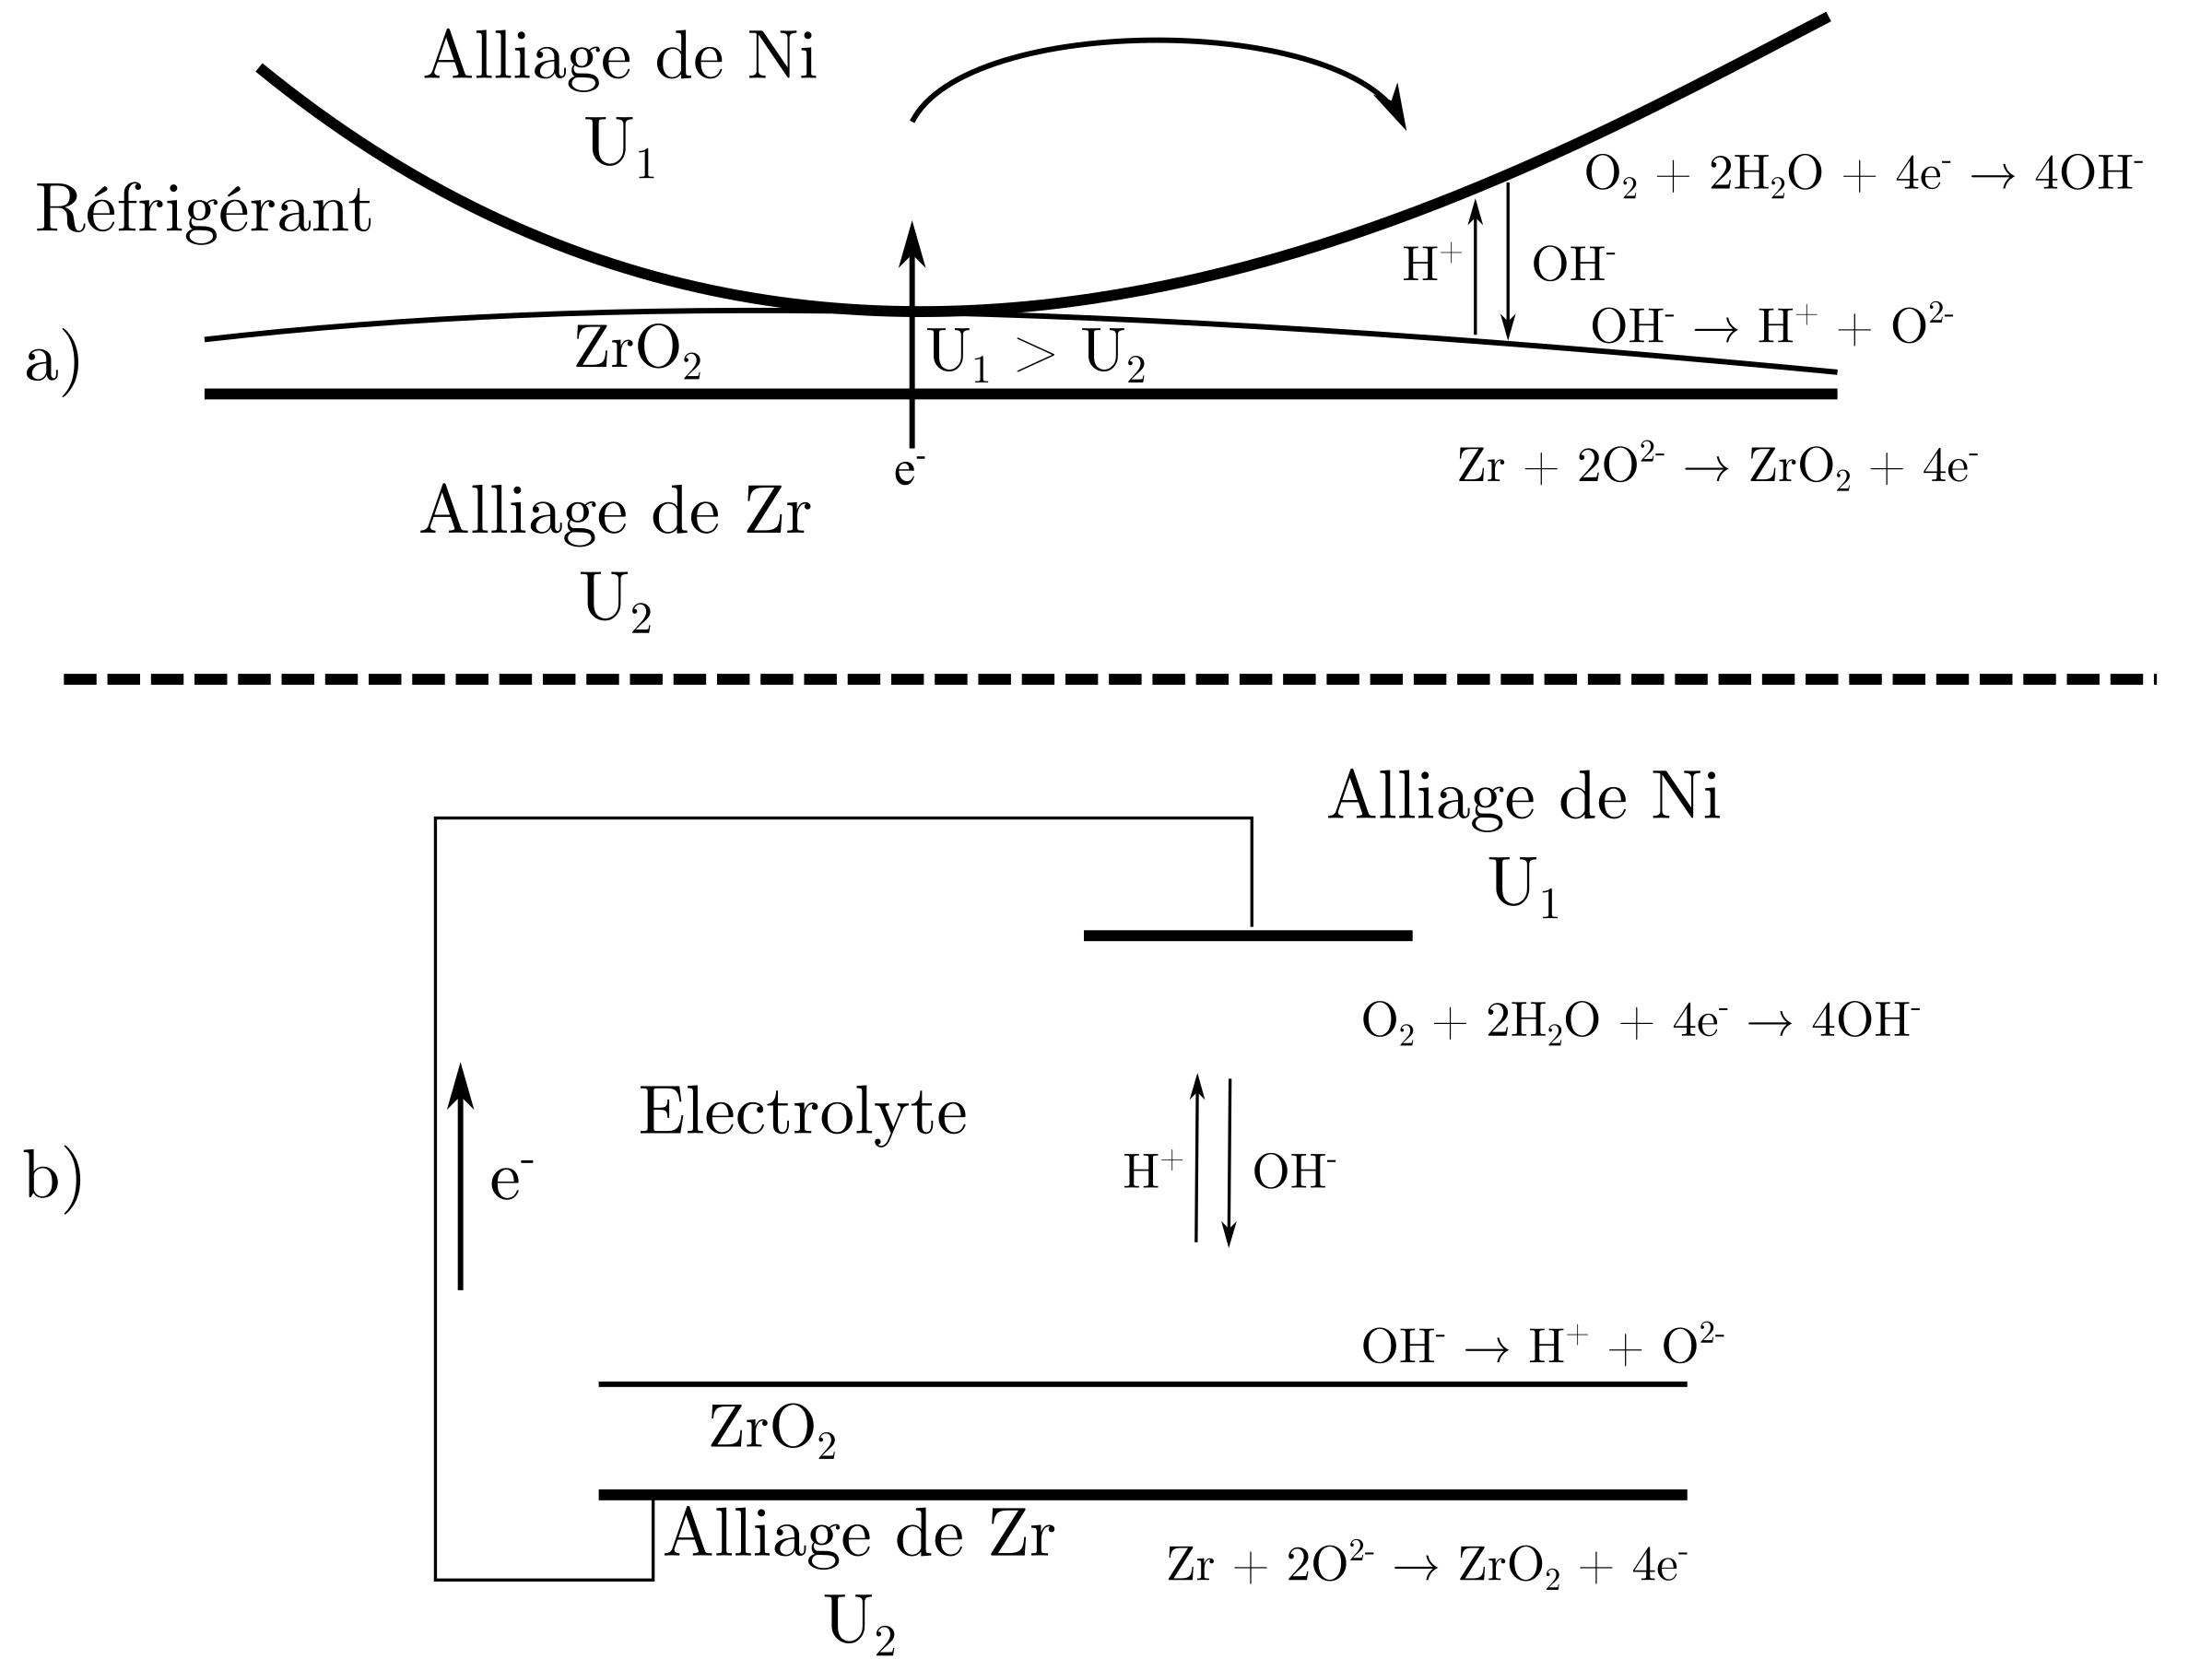
\includegraphics[width=0.85\textwidth]{Lysell_2004-Mechanism-1.png}
            \caption[Représentation schématique du mécanisme couplage galvanique: 
            a) représentation schématique du système réel au niveau du contact entre
            le ressort de la grille de maintien et la gaine de confinement, 
            b) représentation schématique sous forme de circuit électrique équivalent du système de couplage.]
            {Représentation schématique du
                mécanisme de couplage galvanique (d'après \citet{Lysell2004}): 
            a) représentation schématique du système réel au niveau du contact entre
            le ressort de la grille de maintien et la gaine de confinement, 
            b) représentation schématique sous forme de circuit électrique équivalent du système de couplage.} 
            \label{fig:lysell_mechanism} 
 	\end{figure}


    Le mécanisme de couplage galvanique proposé par Lysell permet d’expliquer la diminution d’épaisseur de l’oxyde en
    fonction de la distance entre les électrodes car la chute de potentiel dans l’électrolyte augmente avec la distance.
    Les radiations ont pour effet d’accélérer le processus en augmentant la conductivité électronique
    des oxydes qui se forment sur la
    gaine de confinement et sur les grilles de maintien et elles accélèrent le passage du courant dans l'alumine. 
    Mais les effets de la radiolyse de l’eau ne sont pas pris en compte
    dans ce mécanisme.

    Ce mécanisme est aujourd'hui assez largement admis dans la communauté scientifique du nucléaire.
    Il faut tout de même noter que le transport ionique dans la couche de zircone est
    certainement un élément à prendre en compte, car le courant
    galvanique global sera fixé par le transport ionique dans la couche de zircone si ce dernier est limitant par rapport au
    transport électronique.


       
    \subsection{Radiolyse locale}\label{subsec:local_radiolysis}
    \citet{Ramasubramanian2004} a proposé un mécanisme basé sur la radiolyse locale en postulant que le contact
    électrique, nécessaire dans le mécanisme de couplage galvanique, n’est pas assuré. Ramasubramanian base son
    mécanisme sur l’alignement des niveaux d’énergies de la zircone et du platine avec ceux des couples redox issues de
    la radiolyse de l’eau. Le peroxyde d’hydrogène est un élément clé de son mécanisme puisque c’est un des produits
    principaux de la radiolyse de l’eau \citep{Saffre2011}. Selon l'auteur, le même raisonnement peut être appliqué à
    l'alliage de nickel en lieu et place du platine.

    Le peroxyde d’hydrogène peut s’oxyder à la surface du platine, et les produits de l’oxydation vont être réduits sur
    la zircone à la surface de la gaine comme schématisé en figure \ref{fig:ramasubramanian_mechanism}. La réduction à
    la surface de la gaine crée un "appel d’électrons" accélérant ainsi l’oxydation de la gaine. La force motrice de ce
    mécanisme est la différence de potentiel entre la gaine et la contre-électrode qui provoque la migration des ions
    $\rm H^+$ soumis au champ électrique.

    La remarque faite à la fin du paragraphe \ref{subsec:galvanic_coupling} peut être à nouveau
    formulée concernant les travaux de Ramasubramanian.

    \begin{figure}[H] 
 		\centering 
 		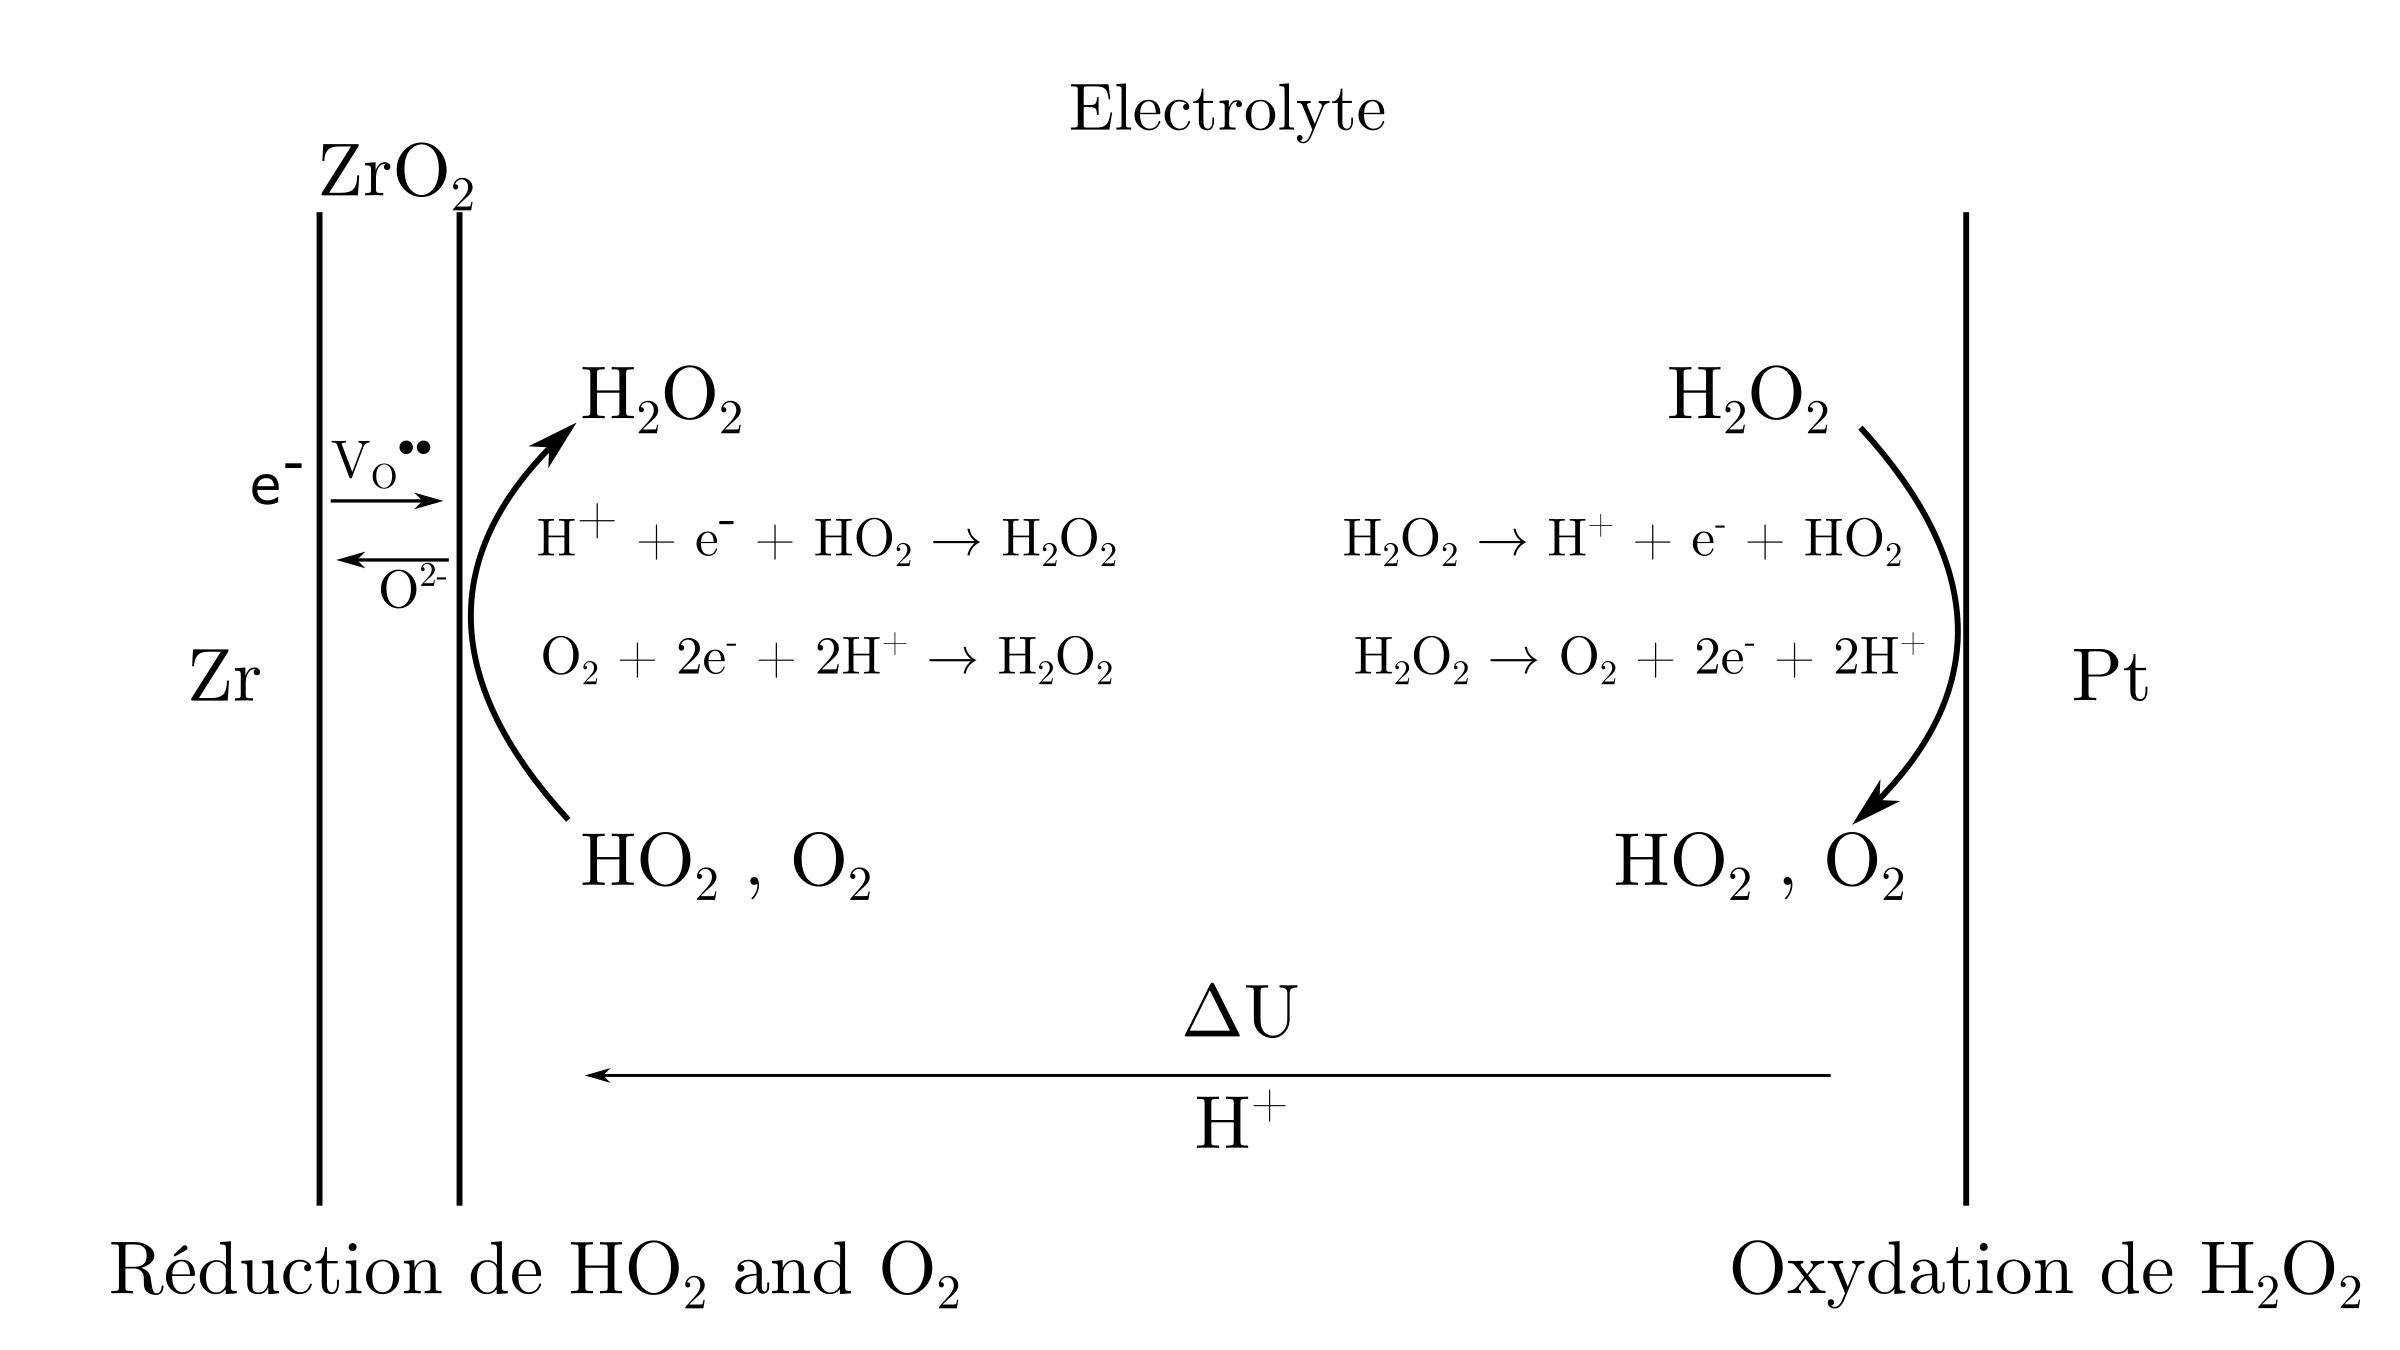
\includegraphics[width=0.75\textwidth]{Ramasubramanian_2004-Mechanism.png}
        \caption[Représentation schématique du mécanisme de radiolyse locale.]
        {Représentation schématique du mécanisme de radiolyse locale (d'après \citet{Ramasubramanian2004}).} 
 		\label{fig:ramasubramanian_mechanism} 
 	\end{figure}

       

	
%%%%%%%%%%%%%%%%%%%%%%%%%%%%%%%%%%%%%%%%%%%%%%%%%%%%%%%%%%%%%%%%%%%%%%%%%%%%%%%%%%%%%
%%%%%%%%%%%%%%%%%%%%%%%%%%%%%%%%%%%%%%%%%%%%%%%%%%%%%%%%%%%%%%%%%%%%%%%%%%%%%%%%%%%%%
\section{Etude expérimentale de la Shadow Corrosion hors réacteur}\label{sec:out_of_pile_experiments}

    Plus récemment, une étude expérimentale hors réacteur a été réalisée par
    \citet{Kim2010}. Les auteurs postulent que la lumière UV est responsable de
    modifications de comportement électrochimique des matériaux alors que les
    rayonnements plus intenses, par exemple les rayonnements $\gamma$, impactent
    principalement les propriétés physiques des matériaux. Effectivement, des rayonnements UV sont
    présents dans le coeur du réacteur à cause du rayonnement de Cherenkov, et, 
    comme mentionné dans le paragraphe \S\ref{subsec:with_irradiation}. \citet{Cox1989} a suggéré que l’effet de l’irradiation
    dans le coeur pouvait éventuellement être simulé avec de la lumière UV à condition que
    son énergie soit supérieure à la largeur de bande interdite de la zircone, soit \SI{5}{\electronvolt} ($\rm \lambda <
    \SI{248}{\nano\meter}$). 

    \subsection{Conditions expérimentales des essais}

    Les principaux alliages testés dans cette étude sont l’alliage Zircaloy-2, l’alliage de nickel X750 et
    l’acier inoxydable 304. Les mesures électrochimiques ont été réalisées dans un autoclave équipé d’une fenêtre en saphir
    monocristallin pour permettre le passage de la lumière et connecté à une boucle de contrôle de la chimie comme illustré 
    en figure \ref{fig:kim_autoclave}. La source lumineuse est une lampe à vapeur de mercure dont le faisceau lumineux est
    guidé jusqu'à la fenêtre de saphir par une
    fibre optique. La lumière émise par cette lampe est intense, et polychromatique avec un spectre allant d'environ 
    \SI{200}{\nano\meter} à l'infrarouge. Dans la suite, l'illumination avec cette lampe sera désignée par illumination
    UV--Visible. 


        \begin{figure}[H] 
            \centering 
            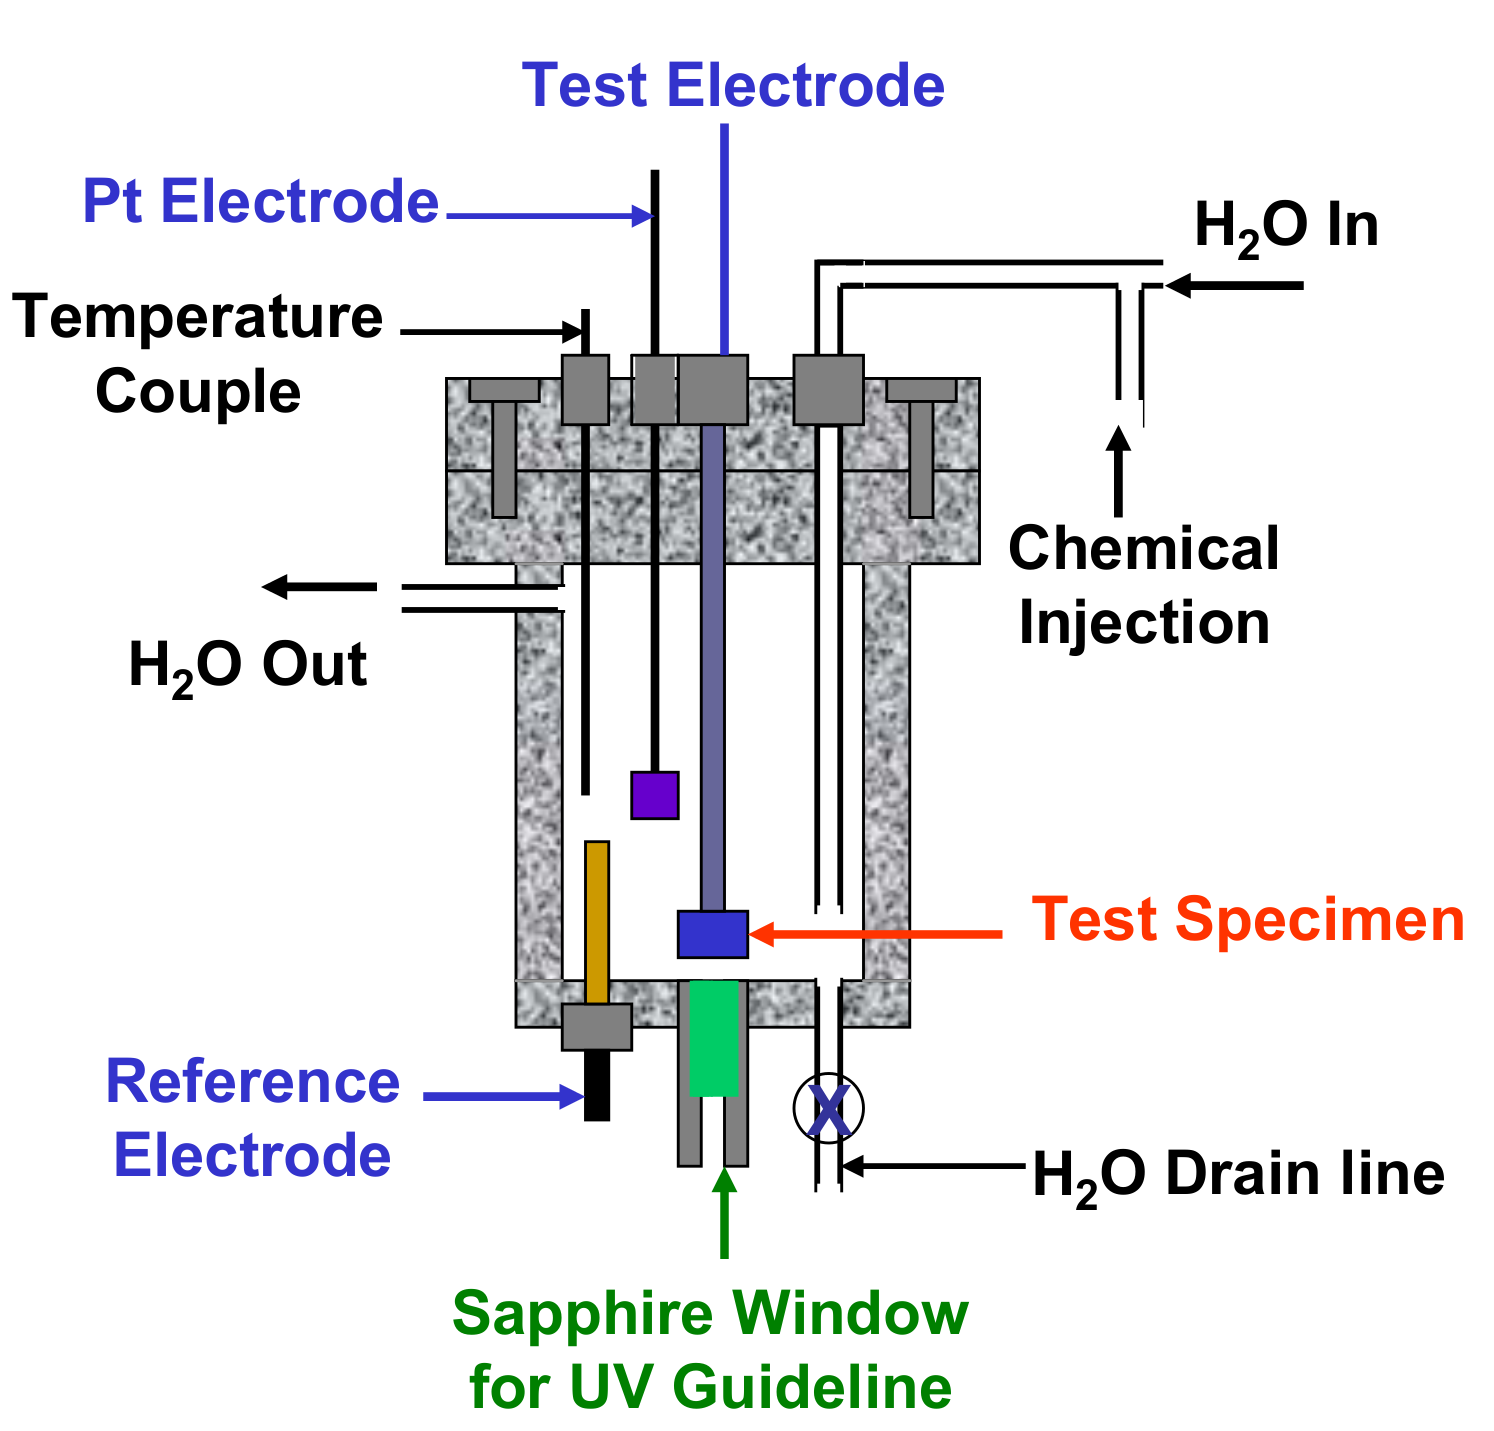
\includegraphics[width=0.5\textwidth]{Kim_2010_Fig2.png} 
            \caption[Représentation schématique de l'autoclave équipé d'un hublot.]
            {Représentation schématique de l'autoclave équipé d'un hublot \citep{Kim2010}.} 
            \label{fig:kim_autoclave} 
        \end{figure}

    \subsection{Résultats}

    La figure~\ref{fig:kim_ecp_vs_time_H2_O2} montre l’évolution des potentiels électrochimiques des différents
    matériaux selon que l’électrolyte contient \SI{0.15}{\ppm} de $\rm H_2$ ou \SI{1.1}{\ppm} d’$\rm O_2$. Dans un
    environnement peu oxydant, soit \SI{0.15}{\ppm} de $\rm H_2$, tous les matériaux présentent des potentiels
    électrochimiques similaires. Lorsque l’environnement est plus oxydant, soit \SI{1.1}{\ppm} d’$\rm O_2$, des
    différences notables apparaissent en termes de valeurs de potentiel électrochimique : le potentiel du Zircaloy-2 est
    plus cathodique que celui des autres matériaux. Ce premier résultat suggère que le phénomène de Shadow Corrosion
    peut être potentiellement une conséquence de la séparation des potentiels en milieu oxygéné caractéristique des REB.
    \citet{Cox2005} suggère que l’ajout de $\rm H_2$ à hauteur de 10~$\rm cc \, kg^{-1}$ pourrait éliminer l’apparition de la Shadow
    Corrosion en fixant le potentiel électrochimique des matériaux au potentiel de l’hydrogène.

    \begin{figure}[H] 
            \centering 
            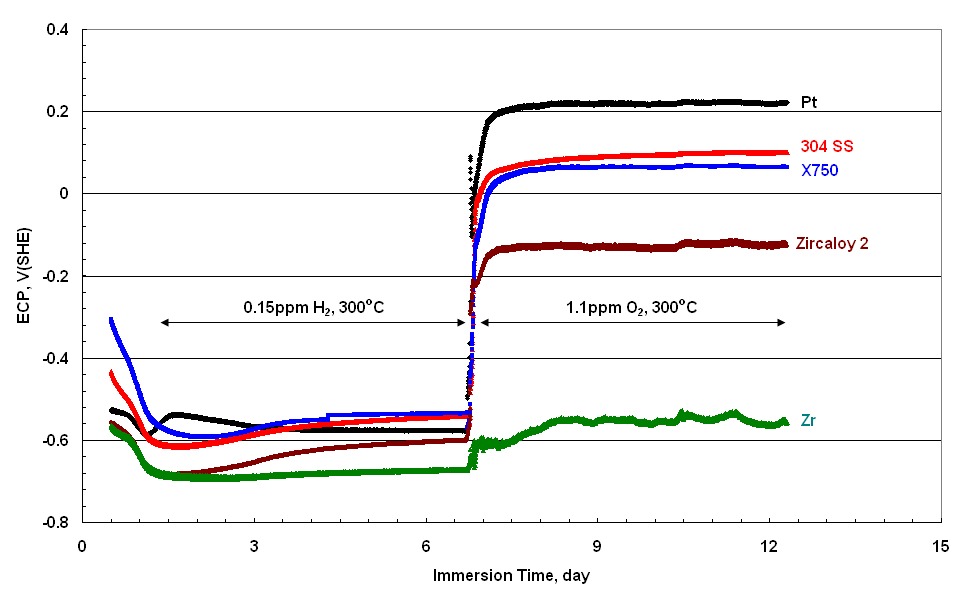
\includegraphics[width=0.85\textwidth]{Kim_2010_Fig3.png} 
            \caption[Evolution des potentiels électrochimiques de l’alliage Zircaloy-2, de l’acier inoxydable 304,
            de l’alliage de nickel X750 et du Pt dans l'eau à \Tkim\ contenant \SI{0.15}{\ppm} de \Hyd\ ou \SI{1.1}{ppm}
        d’\Oxy.]
            {Evolution des potentiels électrochimiques de l’alliage Zircaloy-2, de l’acier inoxydable 304,
            de l’alliage de nickel X750 et du Pt dans l'eau à \Tkim\ contenant \SI{0.15}{\ppm} de \Hyd\ ou \SI{1.1}{ppm}
        d’\Oxy \citep{Kim2010}.} 
            \label{fig:kim_ecp_vs_time_H2_O2} 
        \end{figure}


    La figure~\ref{fig:kim_ecp_vs_time_O2_UV} présente l’évolution des potentiels électrochimiques de l’alliage 
    Zircaloy-2 et de l’alliage de nickel X750 sous illumination UV--Visible intermittente. Le potentiel du Zircaloy-2 diminue vers
    des valeurs plus cathodiques alors que le potentiel de l’alliage X750 augmente vers des valeurs plus anodiques.
    Cette
    variation des potentiels électrochimiques augmente ainsi la différence de potentiel entre les matériaux et par
    conséquent l'intensité d'un éventuel couplage galvanique comme
    illustré en figure~\ref{fig:kim_current_vs_time_O2_UV}. Le sens de variation des potentiels électrochimiques
    sous illumination UV--Visible indique que la couche zircone présente une semiconduction de type \emph{n} alors que l’oxyde 
    formé sur l’alliage X750 présente une semiconduction de type \emph{p} \citep{Memming2008}.
    Cependant, la normalisation
    par rapport à la surface de l'échantillon de Zircaloy-2 (\SI{\sim 1.6}{\square\centi\meter}) des courants de couplage
    mesurés sur la figure \ref{fig:kim_current_vs_time_O2_UV}, fait apparaître des densités de courants ne dépassant
    pas la barre des \SI{1}{\micro\ampere\per\square\centi\meter} dans le cas du couple Zircaloy-2/X750 et donc la
    densité de courant de couplage sous illumination UV--Visible 
    n'est pas supérieure aux valeurs typiques qui sont mesurables en autoclave (\S\ref{subsubsec:oxidation_kinetics}, figure
    \ref{fig:Zy2_Kinetics_vs_T_J}).

    
    \begin{figure}[H] 
        \centering 
        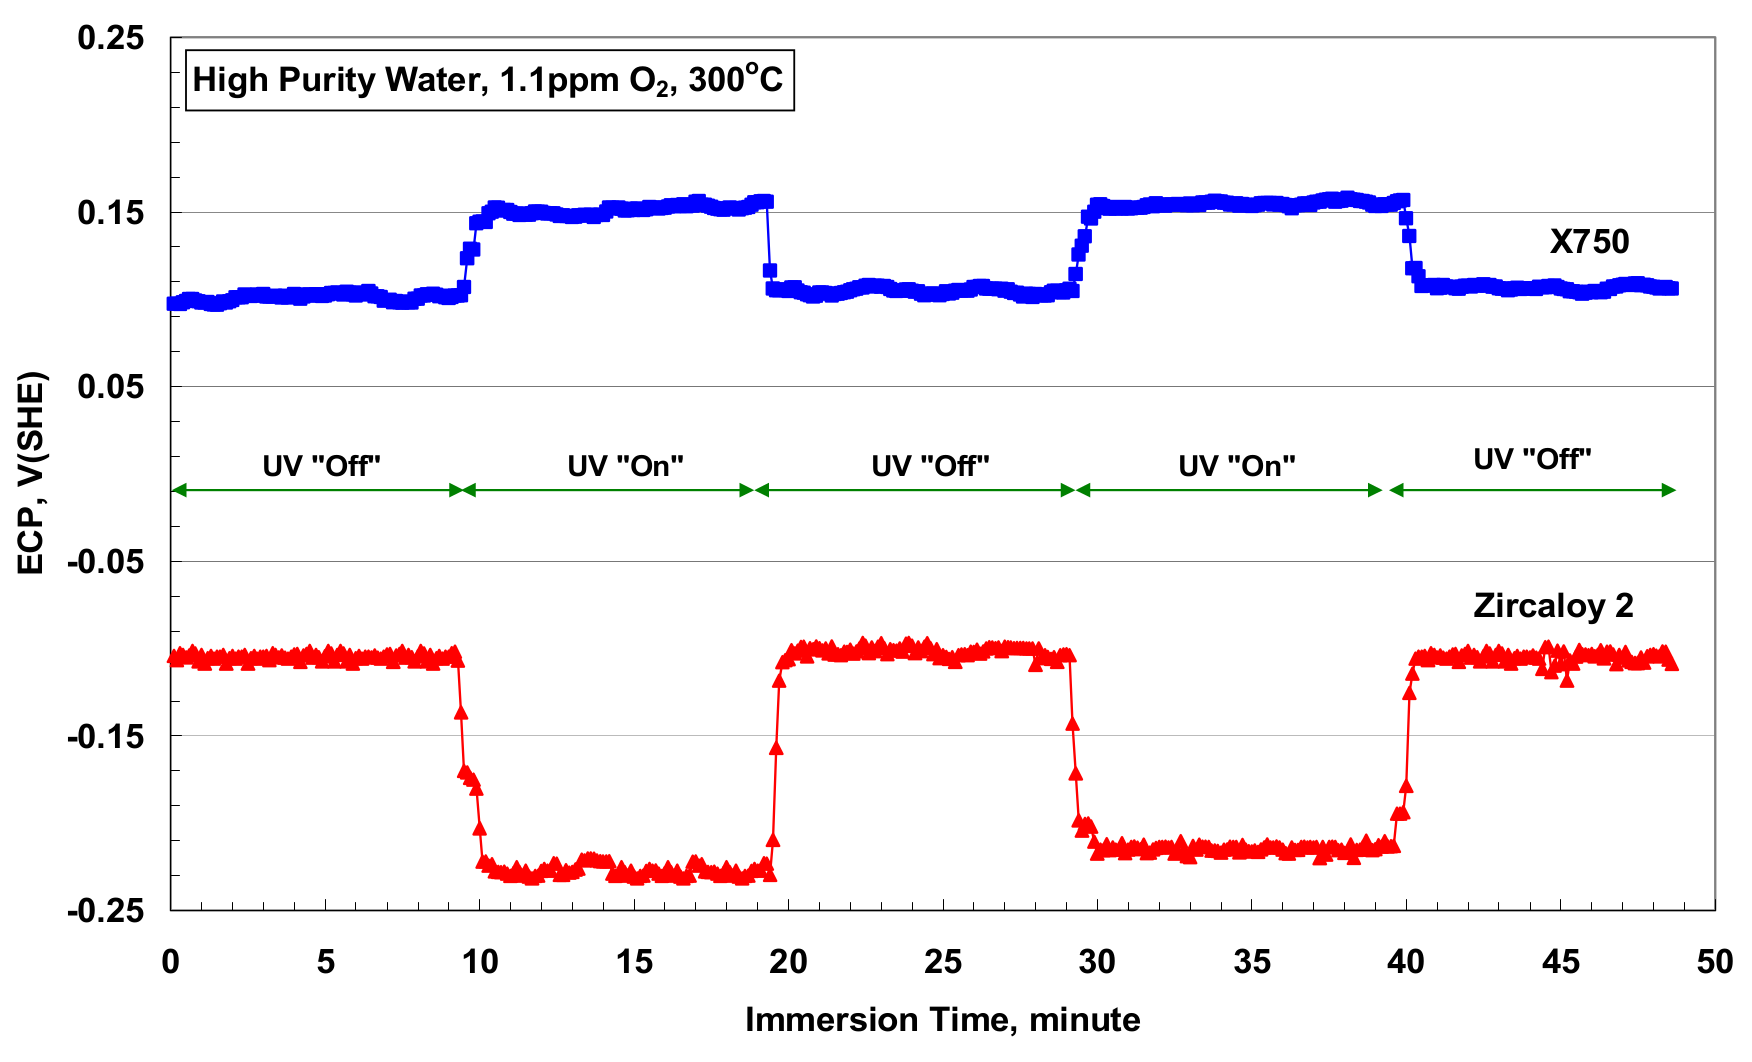
\includegraphics[width=0.85\textwidth]{Kim_2010_Fig6.png} 
        \caption[Potentiels électrochimiques mesurés sur les alliages Zircaloy-2 et X750 dans l'eau à
        \SI{300}{\degreeCelsius} contenant \SI{1.1}{ppm} d'oxygène avec ou sans illumination UV--Visible.]
        {Potentiels électrochimiques mesurés sur les alliages Zircaloy-2 et X750 dans l'eau à
        \SI{300}{\degreeCelsius} contenant \SI{1.1}{ppm} d'oxygène avec ou sans illumination UV--Visible \citep{Kim2010}.} 
        \label{fig:kim_ecp_vs_time_O2_UV} 
    \end{figure}

    \begin{figure}[H]
        \centering
        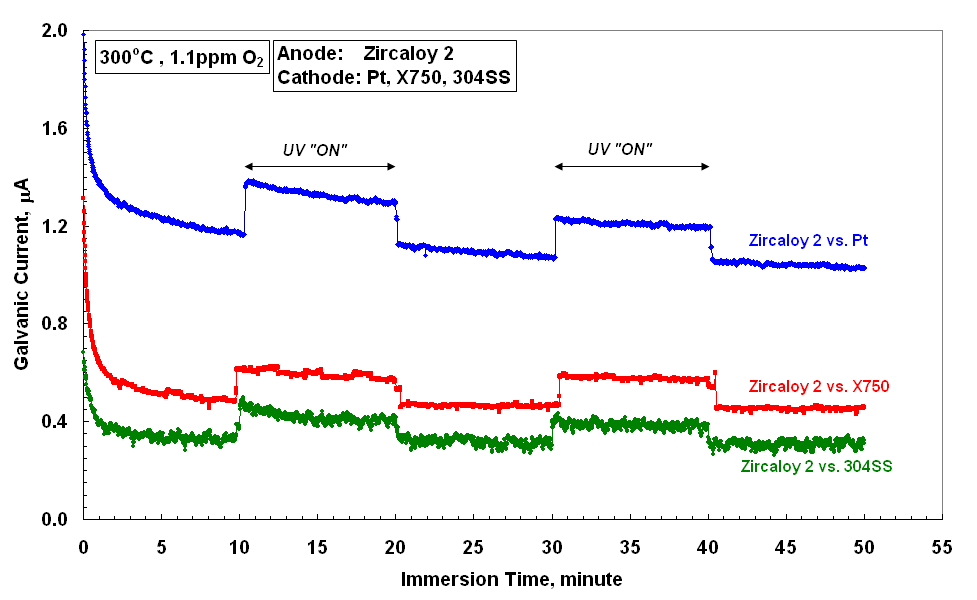
\includegraphics[width=0.85\textwidth]{Kim_2010_Fig13.png} 
        \caption[Courants de couplage mesurés pour les couples Zircaloy-2/X750, Zircaloy-2/Pt et Zircaloy-2/304SS dans l'eau à
        \SI{300}{\degreeCelsius} contenant \SI{1.1}{ppm} d'oxygène avec ou sans illumination UV--Visible.]
        {Courants de couplage mesurés pour les couples Zircaloy-2/X750, Zircaloy-2/Pt et Zircaloy-2/304SS dans l'eau à
        \SI{300}{\degreeCelsius} contenant \SI{1.1}{ppm} d'oxygène avec ou sans illumination UV--Visible \citep{Kim2010}.} 
        \label{fig:kim_current_vs_time_O2_UV} 
    \end{figure}

    L’auteur n’étudie pas l’influence de la longueur d'onde (l’énergie) de la lumière incidente sur la réponse
    en termes de potentiel et de courant. 
    La zircone est l'oxyde majoritaire qui se forme sur la surface de l'alliage Zircaloy-2. 
    Néanmoins, des oxydes minoritaires y sont
    également présents tels que des oxydes de fer, de chrome et/ou spinelles dont les largeurs de bande interdite sont
    inférieures à celle de la zircone \citep{Atmani2008,Loucif2013}. Dans le cas des alliages de nickel, la couche
    d'oxyde est duplex avec une couche interne riche en chrome et une couche externe formée de spinelle de
    nickel, fer et chrome \citep{Marchetti2006}.
    Par conséquent, l’illumination UV--Visible modifie également
    le comportement électrochimique de ces oxydes "mineurs". En d’autres termes, la modification de comportement
    électrochimique, sous illumination UV--Visible, observée dans cette étude est la résultante de la contribution de l’oxyde
    majoritaire mais également de la contribution de tous les oxydes minoritaires.
    Une manière de séparer ces différentes contributions est de réaliser des caractérisations par photoélectrochimie
    (communément désignée par PEC) au photopotentiel ou au photocourant.


    Le paragraphe \ref{sec:state_of_art_PEC} qui suit donne les bases théoriques nécessaires à la compréhension de ce
    type de caractérisations, ainsi que quelques exemples d'applications à la caractérisation de couches d'oxydation
    thermiques. Nous y reviendrons plus en détail au chapitre \ref{chap:design}.

    
    

%%%%%%%%%%%%%%%%%%%%%%%%%%%%%%%%%%%%%%%%%%%%%%%%%%%%%%%%%%%%%%%%%%%%%%%%%%%%%%%%%%%%%
%%%%%%%%%%%%%%%%%%%%%%%%%%%%%%%%%%%%%%%%%%%%%%%%%%%%%%%%%%%%%%%%%%%%%%%%%%%%%%%%%%%%%
\section{Caractérisations photoélectrochimiques}\label{sec:state_of_art_PEC}
    
    La photoélectrochimie utilise l'effet photovoltaïque à l'interface entre un semiconducteur et un électrolyte découvert par
    \citet{Becquerel1839} en 1839. La première expérience a été réalisée avec une électrode d'argent sur laquelle une
    couche d'oxyde s'était développée. Cette dernière a été mise dans une solution acide et connectée à une électrode de
    platine. Lors de l'illumination, un photopotentiel et un photocourant ont été observés. Les premières études de
    compréhension des processus physico-chimiques se produisant à l'interface semiconducteur/électrolyte et à l'origine
    de photopotentiel ou de ce photocourant ont été réalisées bien plus tardivement 
    \citep{Gerischer1966, Copeland1942, Stimming1986}. 

    La photoélectrochimie est, aujourd'hui entre autres, un outil de caractérisations \emph{in-situ} \citep{Fujishima1972, Gratzel2001}, 
    ou \emph{ex-situ} \citep{Carpenter1989, Sunseri1995, Boschloo2001} de matériaux semiconducteurs tels que les oxydes
    formés sur les alliages métalliques, les sulfures et les carbures. Cette technique permet de déterminer des
    propriétés optiques et électroniques des semiconducteurs tels que leur largeur de bande interdite ainsi que leur
    type de semiconduction.
    Elle permet également de déterminer des paramètres de l'interface semiconducteur/électrolyte tels que les positions
    des bords de bande au contact de l'électrolyte. 
    
    Les notions de base de la photoélectrochimie sont présentées dans la suite avec des exemples d'application de la photoélectrochimie
    sur des alliages de zirconium et de nickel. Le détail du développement théorique est très largement décrit dans la
    littérature \citep{Marcus2006, Memming2008, Gerischer1985, Morrison1980, Bard2002, Sato1998}.
    On notera que, l'ensemble des notions qui vont être introduites dans la suite 
    font les hypothèses suivantes:
    \begin{itemize}
        \item le semiconducteur est considéré comme idéal c'est-à-dire cristallin, homogène, semi-infini
        \item la constante diélectrique du semi-conducteur ($\epsilon$) est indépendante de la fréquence
        \item l'interface du semiconducteur est plane
        \item la capacité de la couche de Helmholtz ($C_\Hm$) est très grande devant celle de la région de la charge
        d'espace du semiconducteur
        \item la variation de la chute de potentiel dans la couche de Helmholtz en fonction du
        potentiel imposé ou du dopage du semi-conducteur est négligeable.
    \end{itemize}

    Les oxydes ou les films passifs formés sur les alliages, lors du vieillissement de ces derniers, respectent très
    rarement l'ensemble des conditions énoncées ci-dessus, mais la littérature montre que les modèles développés ci-après
    restent souvent applicables approximativement, mais avec profit.


    \subsection{Notions de base sur les semiconducteurs}\label{subsec:basics_semiconductors}
    
    \subsubsection{Structure de bandes électroniques}\label{subsubsec:band_model}

    Les solides sont généralement classés en trois catégories: \emph{conducteurs}, \emph{semiconducteurs} et
    \emph{isolants}.
    Chacune de ces catégories peut être représentée par une structure de bande d'énergie électronique illustrée en figure
    \ref{fig:band_model}. Les bandes de \emph{valence} et de \emph{conduction} sont des bandes d'énergie permises pour les
    électrons. Elles sont séparées par une bande d'énergie nommée \emph{gap} ou \emph{bande interdite} qui ne
    comprend aucun état d'énergie électronique permise: sa largeur est notée $\E_g$. La répartition des électrons dans
    ces
    bandes est décrite par la position du niveau de Fermi noté $\E_F$. Ce dernier représente l'énergie la plus haute que peut occuper
    un électron à \SI{0}{\kelvin}, il est l'équivalent du potentiel électrochimique des électrons dans la phase solide. 
    La plus basse énergie de la bande de conduction est notée $\E_c$ alors que l'énergie
    la plus élevée de la bande de valence est notée $\E_v$.

     \begin{figure}[H]
        \centering
        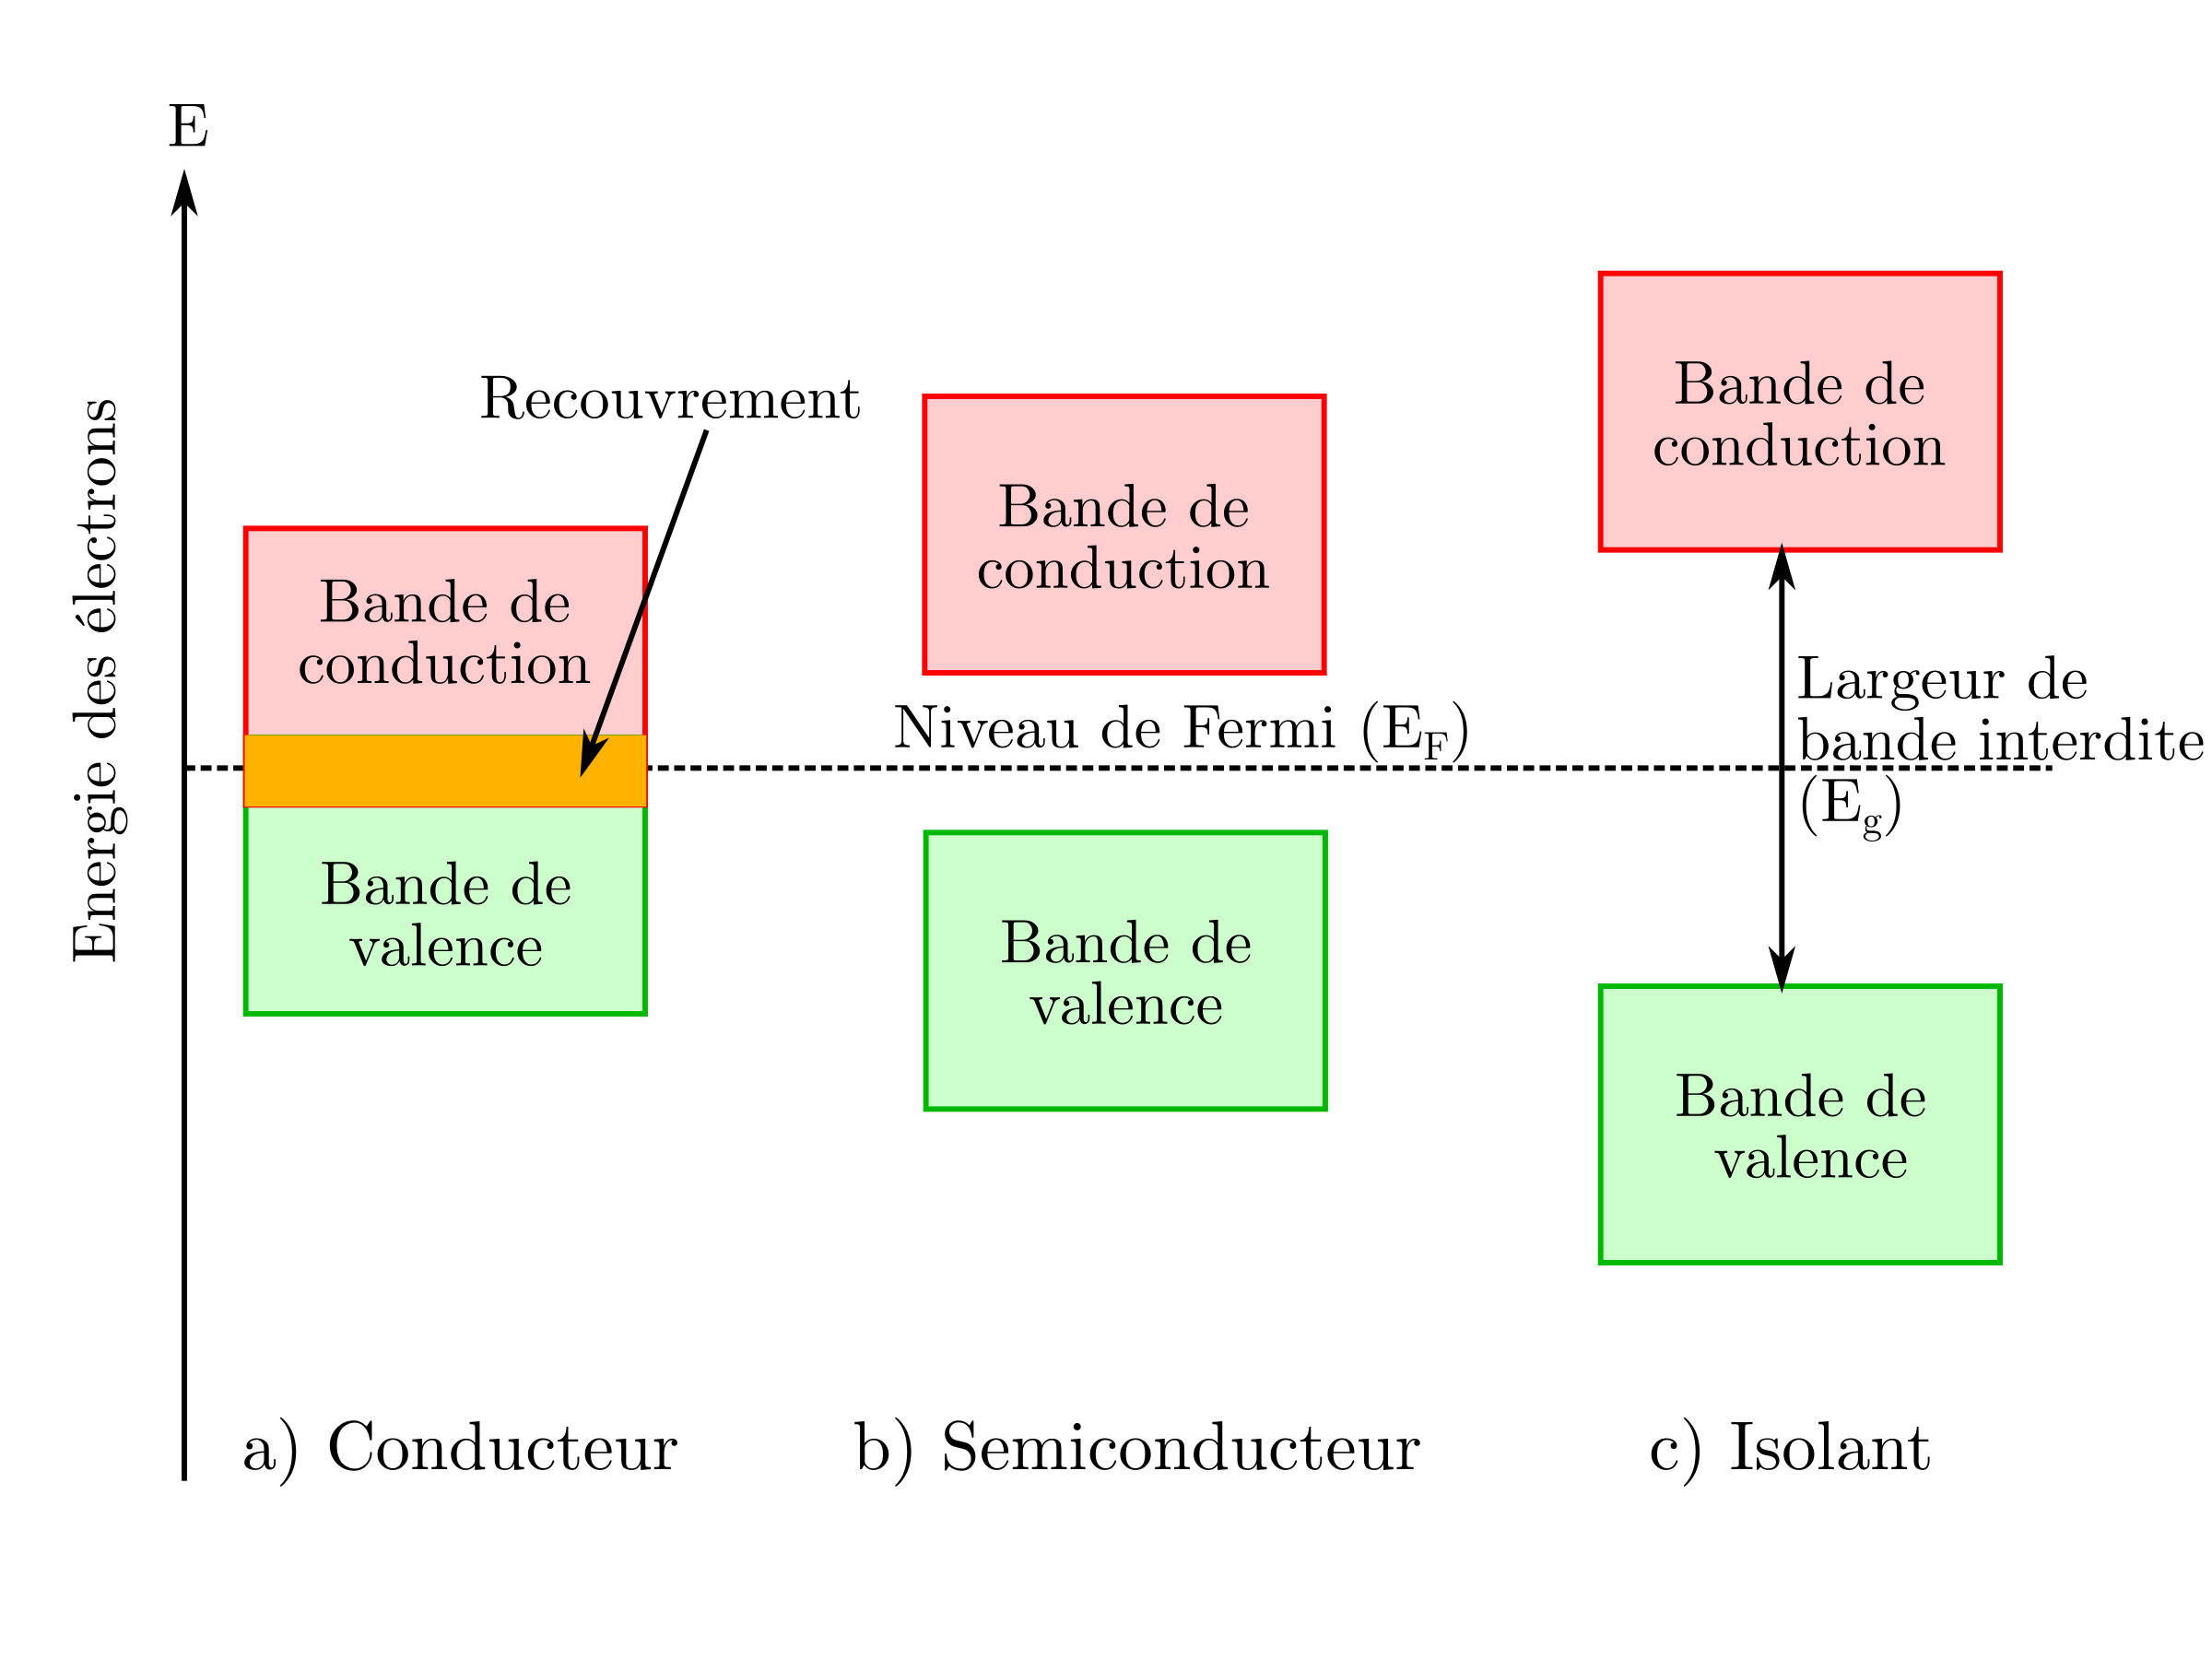
\includegraphics[width=0.65\textwidth]{Band_Model.png}
        \caption[Représentation schématique des structures de bandes électroniques:
        a) conducteur, 
        b) semiconducteur,
        c) isolant.]
        {Représentation schématique des structures de bandes électroniques (d'après \citet{Marucco2006}):
        a) conducteur, 
        b) semiconducteur,
        c) isolant.}
        \label{fig:band_model}
    \end{figure}

    La conduction électronique est due soit aux mouvements, dans la bande de
    conduction, des électrons chargés négativement soit aux mouvements, dans la bande de valence, des trous chargés
    positivement ou bien aux deux simultanément. La conduction électronique dépend donc du nombre de porteurs de charge
    disponibles dans la bande de conduction et dans la bande de valence. 
    Dans le cas d'un conducteur, la bande permise occupée d'énergie la plus élevée est partiellement remplie, on dit
    quelquefois que les bandes de valence et de conduction se trouvent en position de recouvrement.
    La distinction, en termes de conduction électronique, entre un semiconducteur et un isolant est plus floue puisqu'elle 
    dépend de la largeur du gap et de l'énergie apportée par l'environnement aux électrons de la bande de valence pour
    passer dans la bande de conduction. 
    
    Dans les semiconducteurs, les porteurs de charge peuvent être générés de trois manières différentes:
    \emph{excitation thermique}, \emph{photoexcitation} et \emph{dopage}. La figure \ref{fig:excitation_carrier} illustre
    de manière schématique les trois mécanismes de générations des porteurs de charge dans les bandes de valence ou de
    conduction. Pour des gaps faibles,
    l'excitation thermique peut expulser un électron de la bande de valence vers la bande de conduction. Dans le cas de la
    photoexcitation, un électron peut être expulsé de la bande de valence vers la bande de conduction lorsqu'un photon
    incident absorbé possède une énergie supérieure au gap. Le dopage, quant à lui, consiste à introduire des niveaux d'énergie
    supplémentaires situés entre la bande de valence et la bande de conduction.

    \begin{figure}[H]
        \centering
        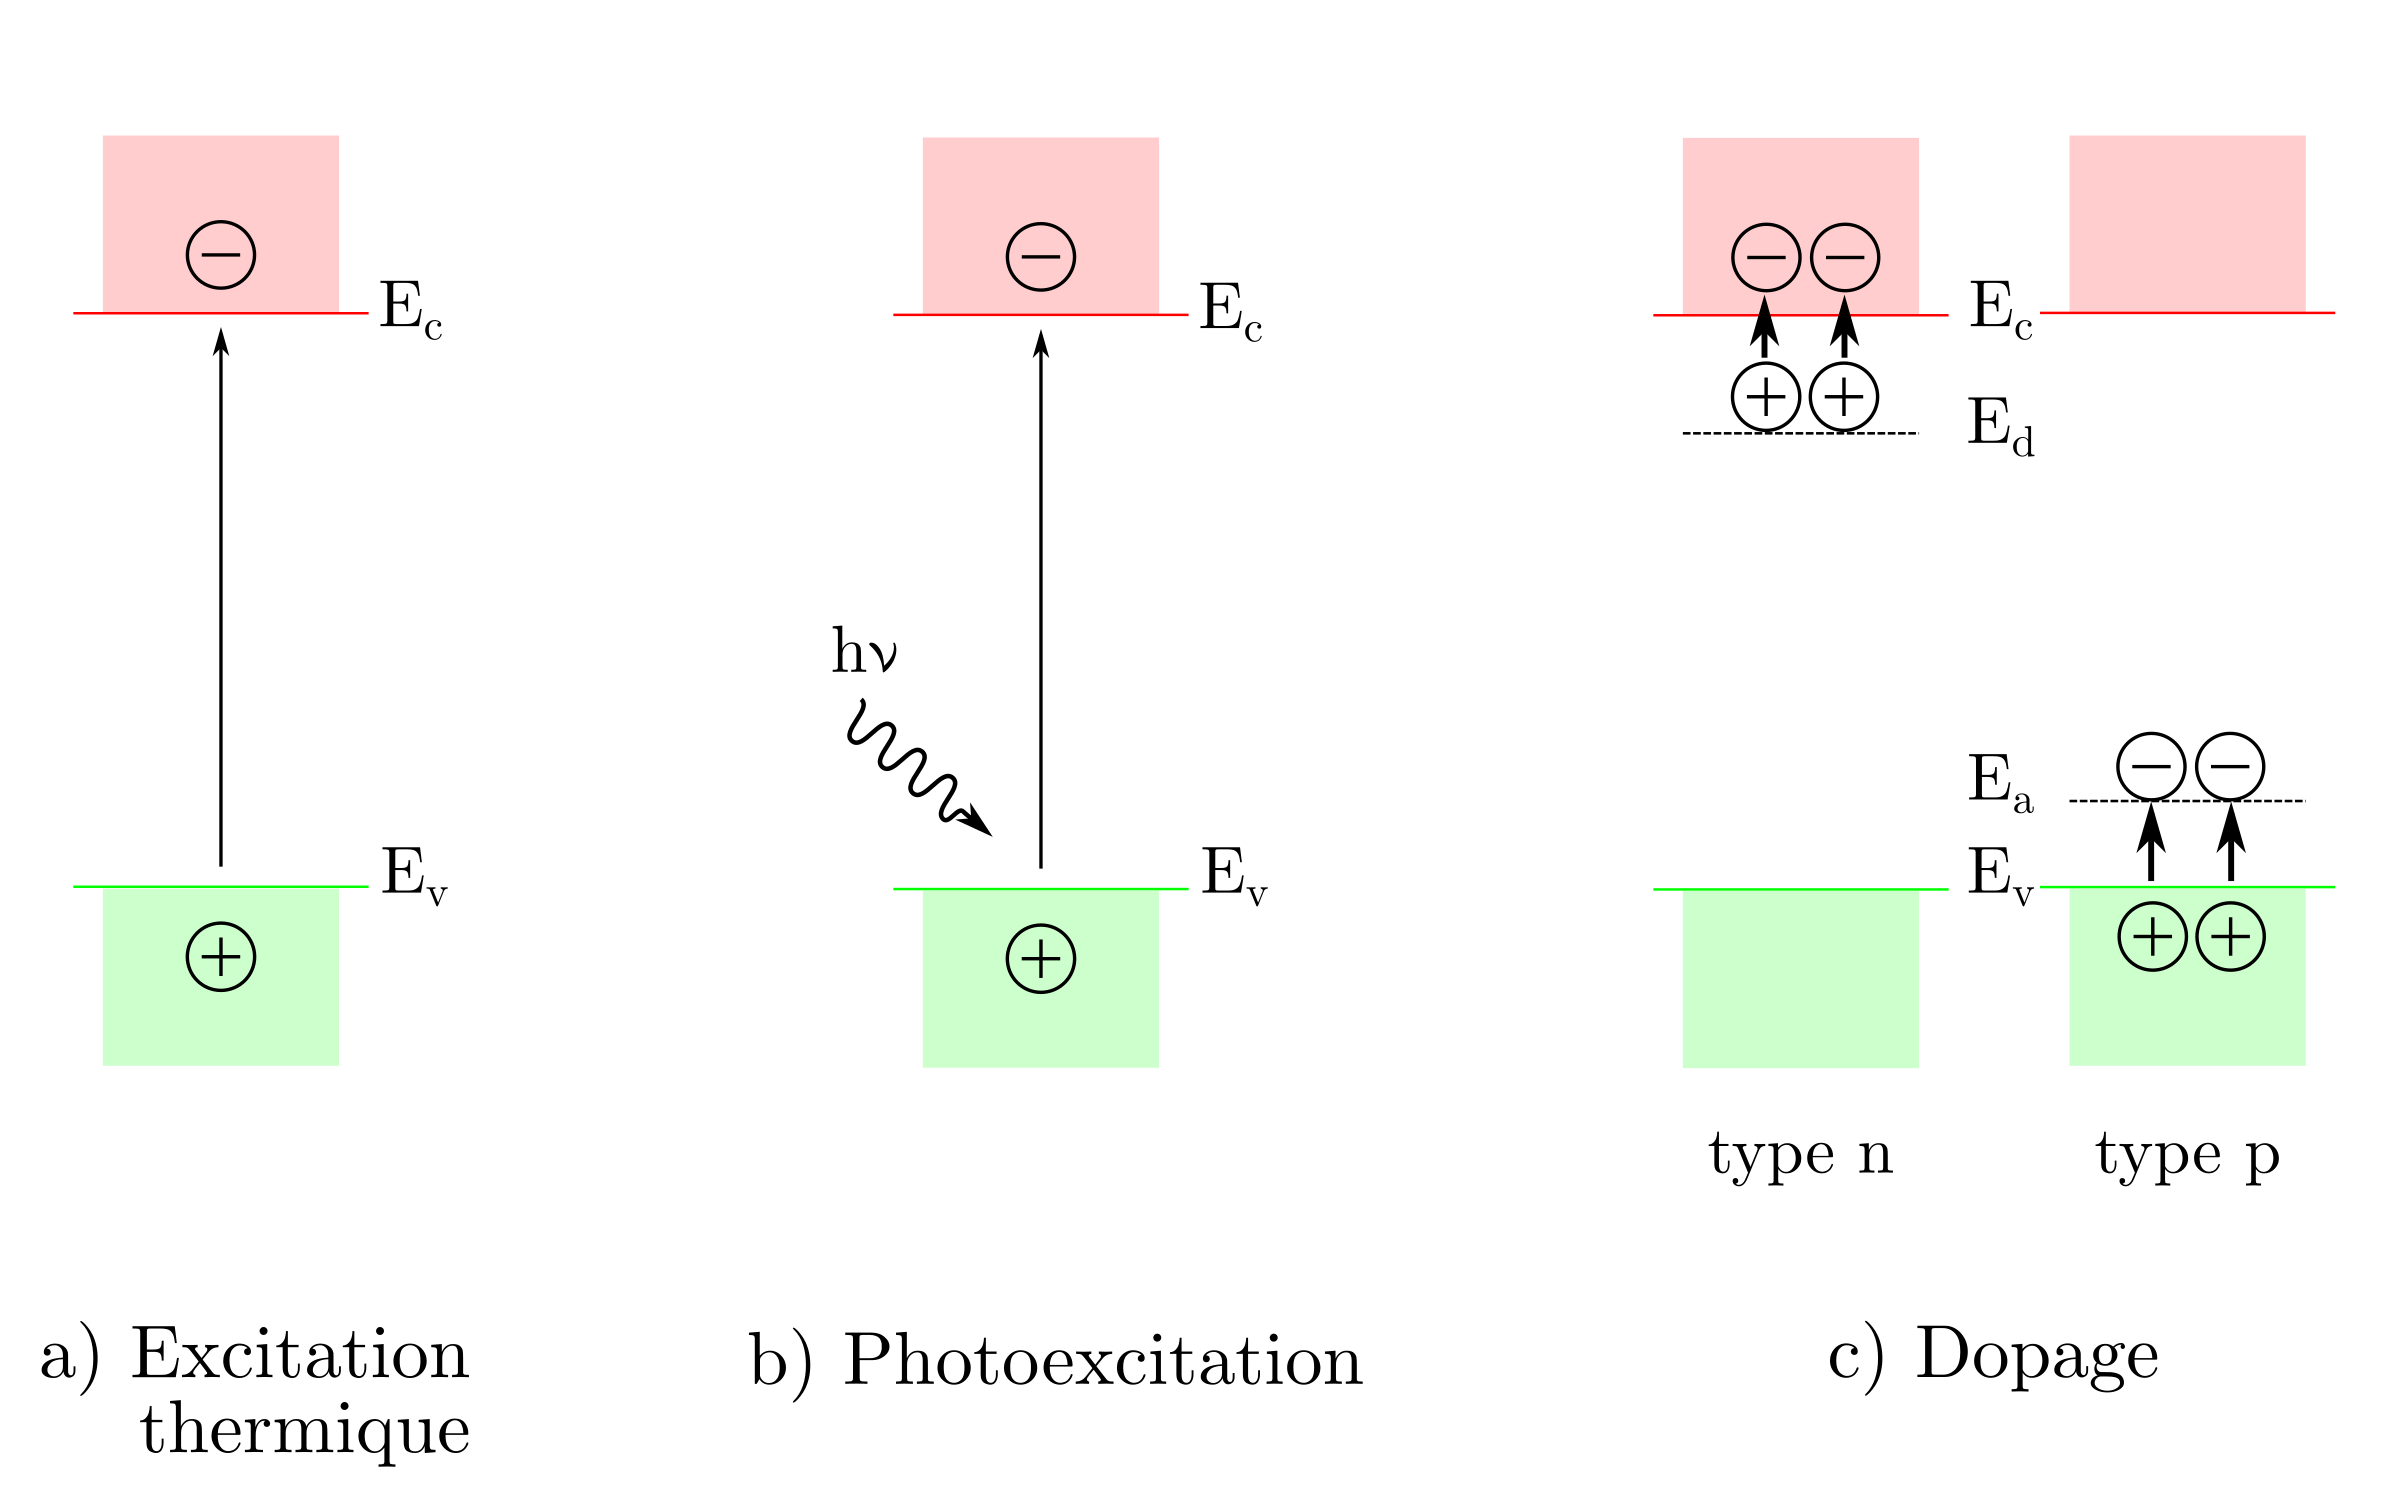
\includegraphics[width=0.85\textwidth]{Excitation_Carrier.png}
        \caption[Représentation schématique des mécanismes de génération des porteurs de charge dans des
        semiconducteurs ou des isolants:
        a) excitation thermique,
        b) photoexcitation,
        c) dopage.]
        {Représentation schématique des mécanismes de génération des porteurs de charge dans des
            semiconducteurs ou des isolants (d'après \citet{Finklea1983}):
        a) excitation thermique,
        b) photoexcitation,
        c) dopage.}
        \label{fig:excitation_carrier}
    \end{figure}

    Le dopage peut être dû à une modification de la stoechiométrie du semiconducteur, ou l'introduction d'impuretés
    dans le réseau du
    semiconducteur. Dans le cas des semiconducteurs de type \emph{n}, les niveaux d'énergie donneurs d'électrons
    $\E_d$ se situent près
    de la bande de conduction. Les électrons des niveaux d'énergie donneurs rejoignent la bande de conduction par
    excitation thermique. Par conséquent, les porteurs de charge majoritaires sont des électrons chargés négativement
    mobiles dans la bande de conduction.
    De manière similaire, les niveaux d'énergie accepteur d'électrons $\E_a$ des semiconducteurs de type \emph{p} se
    situent près de la
    bande de valence. Ces derniers capturent les électrons de la bande de valence créant ainsi des trous. Dans ce cas de
    figure, les porteurs de charge majoritaires sont des trous chargés positivement mobiles dans la bande de valence.
    La classification des semiconducteurs, type \emph{p} ou type \emph{n}, indique donc le signe des porteurs de
    charges mobiles
    majoritaires. Les semiconducteurs non dopés sont appelés semiconducteurs intrinsèques.

    Le niveau de Fermi ($\E_F$) dans les semiconducteurs intrinsèques est situé au milieu du gap. Le dopage de
    type \emph{n} et \emph{p} déplace le niveau de Fermi vers les bords des bandes de conduction $\E_c$ et de valence
    $\E_v$, respectivement.
    La figure \ref{fig:fermi_position} illustre la position du niveau de Fermi en fonction du type de semiconducteur.


     \begin{figure}[H]
        \centering
        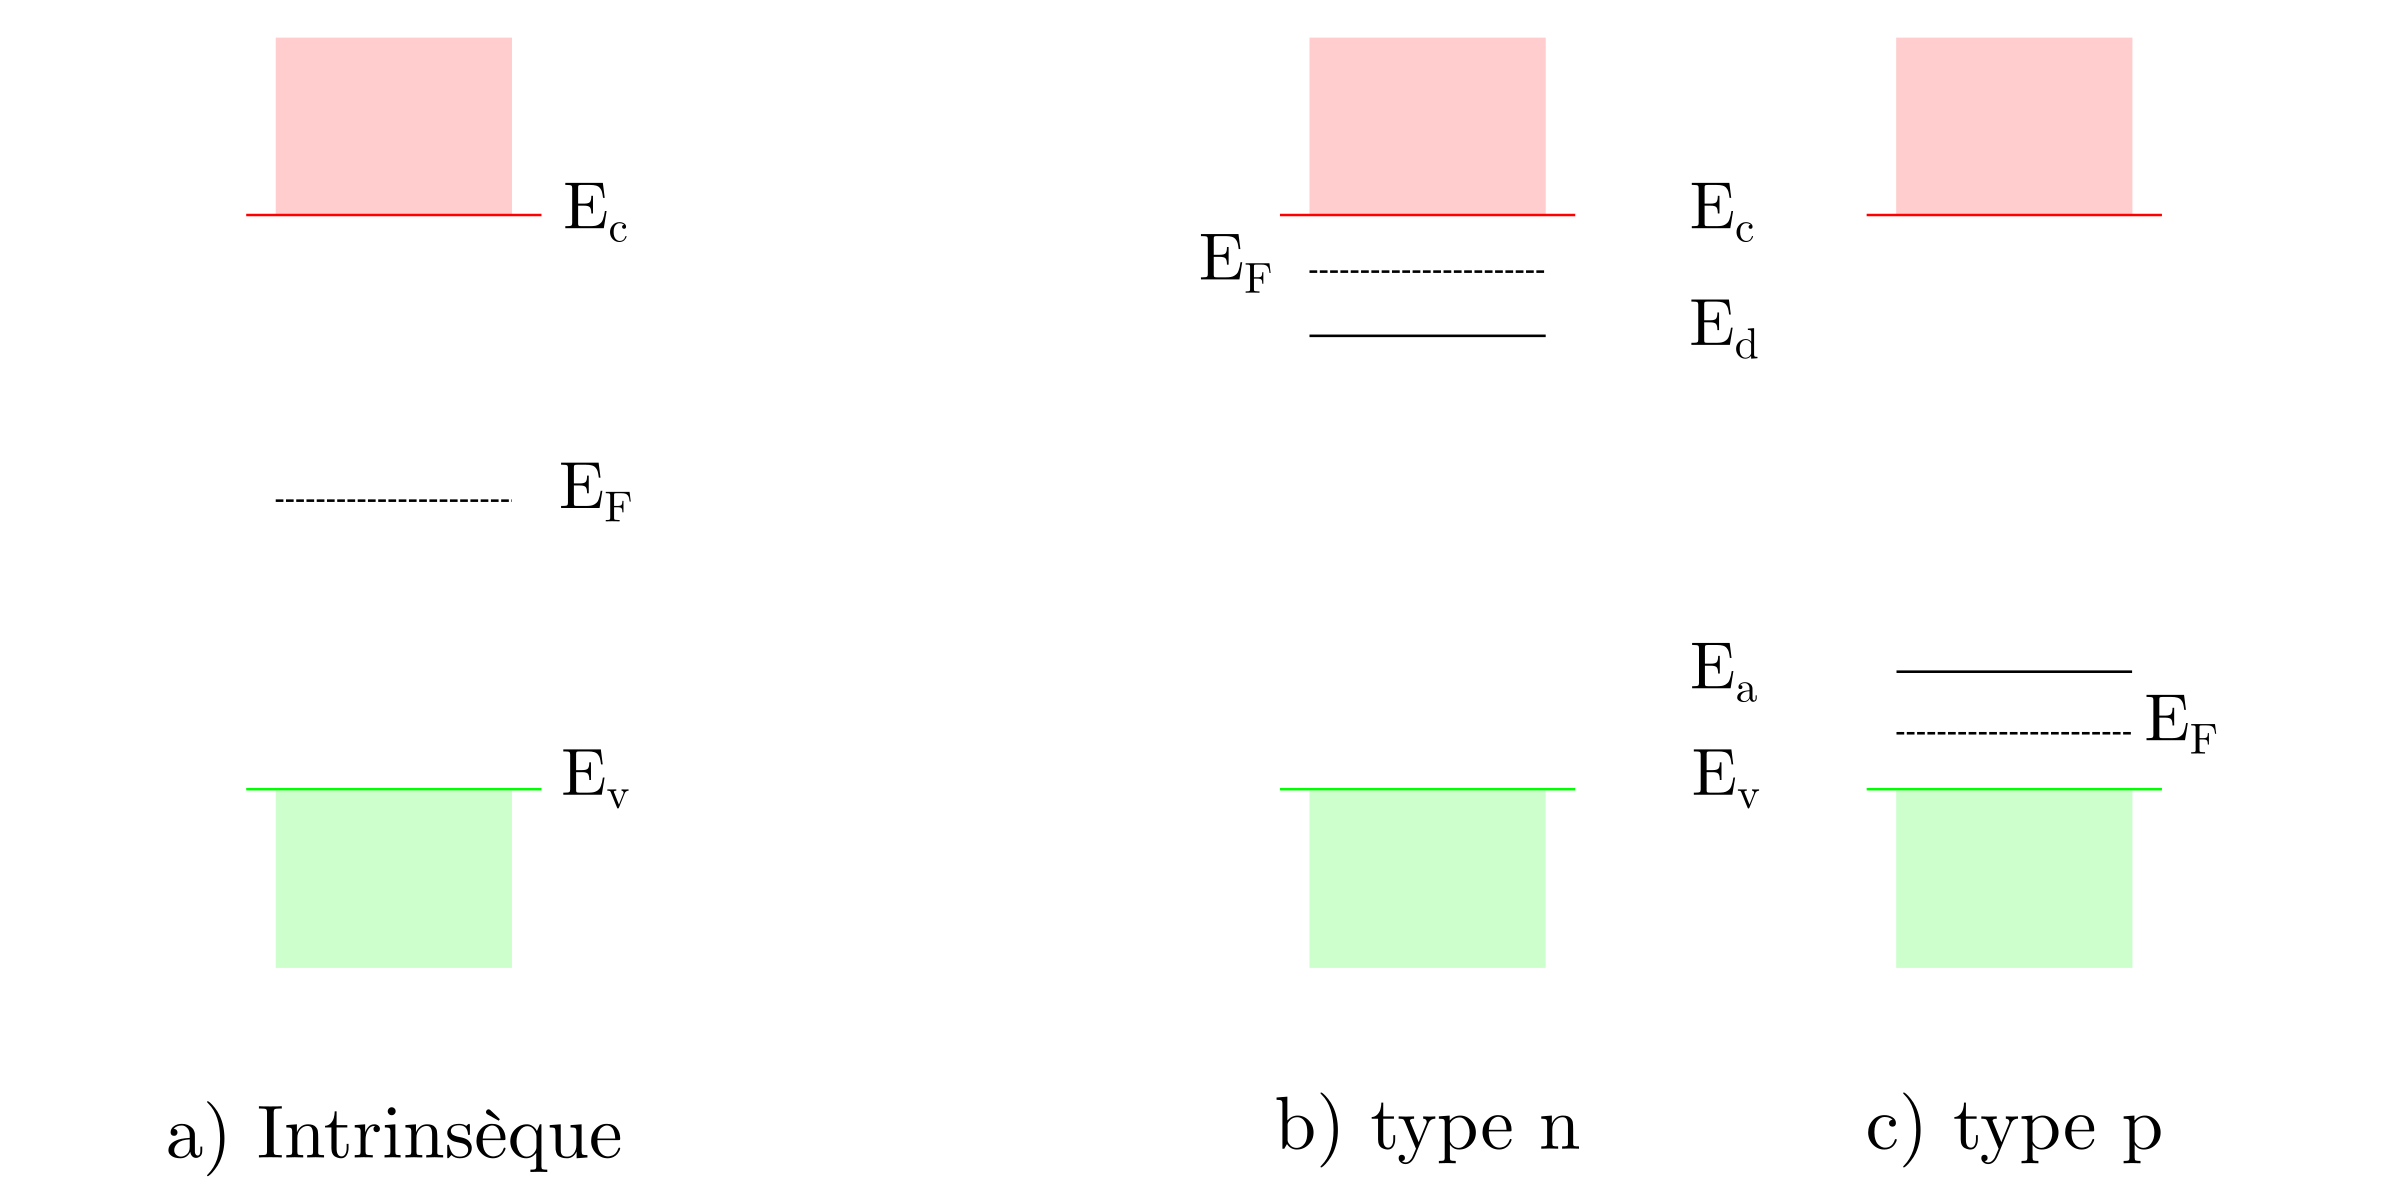
\includegraphics[width=0.85\textwidth]{Fermi_Position.png}
        \caption[Représentation schématique de la position du niveau de Fermi en fonction du type de semiconducteur:
        a) intrinsèque,
        b) type \emph{n},
        c) type \emph{p}.]
        {Représentation schématique de la position du niveau de Fermi en fonction du type de semiconducteur
            (d'après \citet{Finklea1983}):
        a) intrinsèque,
        b) type \emph{n},
        c) type \emph{p}.}
        \label{fig:fermi_position}
    \end{figure}


    
    \subsubsection{Interface semiconducteur/électrolyte à l'obscurité}
    \label{subsec:semiconductor_electrolyte_contact_dark}
     
    Lorsqu'un semiconducteur est mis en contact avec un électrolyte, un gradient de potentiel s'établit à l'interface. Le
    profil du potentiel à l'interface est illustré par la figure \ref{fig:interfacial_potential_gradient}. 
    
    \begin{figure}[H]
        \centering
        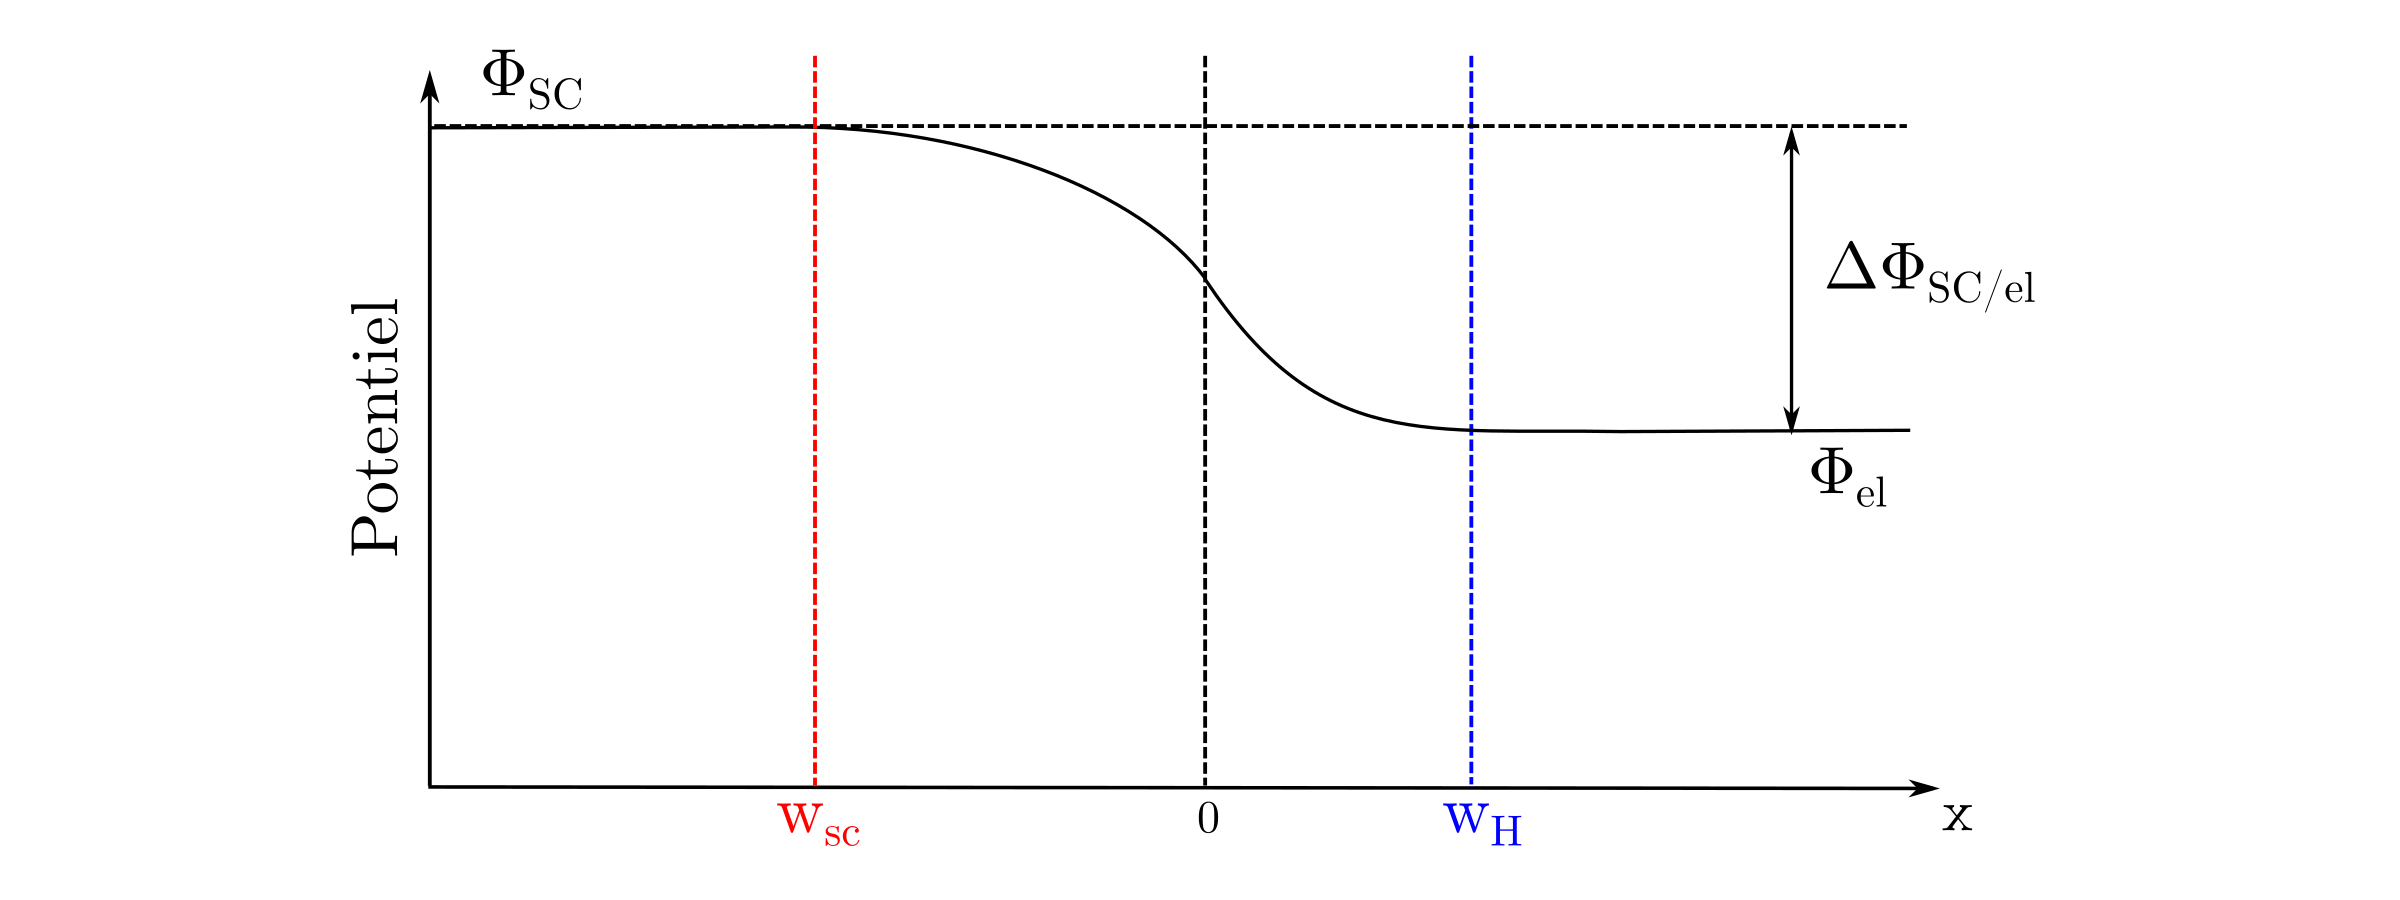
\includegraphics[width=0.85\textwidth]{Interfacial_Potential_Gradient.png}
        \caption[Gradient de potentiel à l'interface semiconducteur/électrolyte.]
        {Gradient de potentiel à l'interface semiconducteur/électrolyte (d'après \citet{Marcus2006}). $\Phi _{\SC}$ et
        $\Phi _{\el}$
        correspondent aux potentiels dans le semiconducteur et l'électrolyte, respectivement. $\Delta \Phi _{\SC/\el}$ correspond à la
        différence de potentiel entre le semiconducteur et l'électrolyte. $w_{\SC}$ et $w_{\Hm}$ correspondent aux
        épaisseurs de la charge d'espace et de la double couche électrochimique, respectivement.}
        \label{fig:interfacial_potential_gradient}
    \end{figure}
    
    En fonction du niveau de Fermi de
    l'électrolyte par rapport aux bords des bandes de valence et de conduction du semiconducteur, le transfert de charge
    transitoire peut mener à trois situations principales. La situation de bande plate est obtenue lorsque le niveau de Fermi
    dans l'électrolyte correspond à celui du semiconducteur. Dans cette situation, il n'y pas de
    gradient de potentiel dans le semiconducteur, on parle de situation de bandes plates. Si les deux niveaux de Fermi
    ne sont pas alignés, une courbure des bandes
    dans le semiconducteur apparaît au voisinage de l'interface semiconducteur/électrolyte. 
    Cette courbure des bandes entraîne soit un appauvrissement soit
    une accumulation des porteurs de charge majoritaires au voisinage de l'interface.
    L'extension spatiale de la zone d'appauvrissement
    ou d'accumulation est appelée région de charge d'espace (figure \ref{fig:bending_example}).

     \begin{figure}[H]
        \centering
        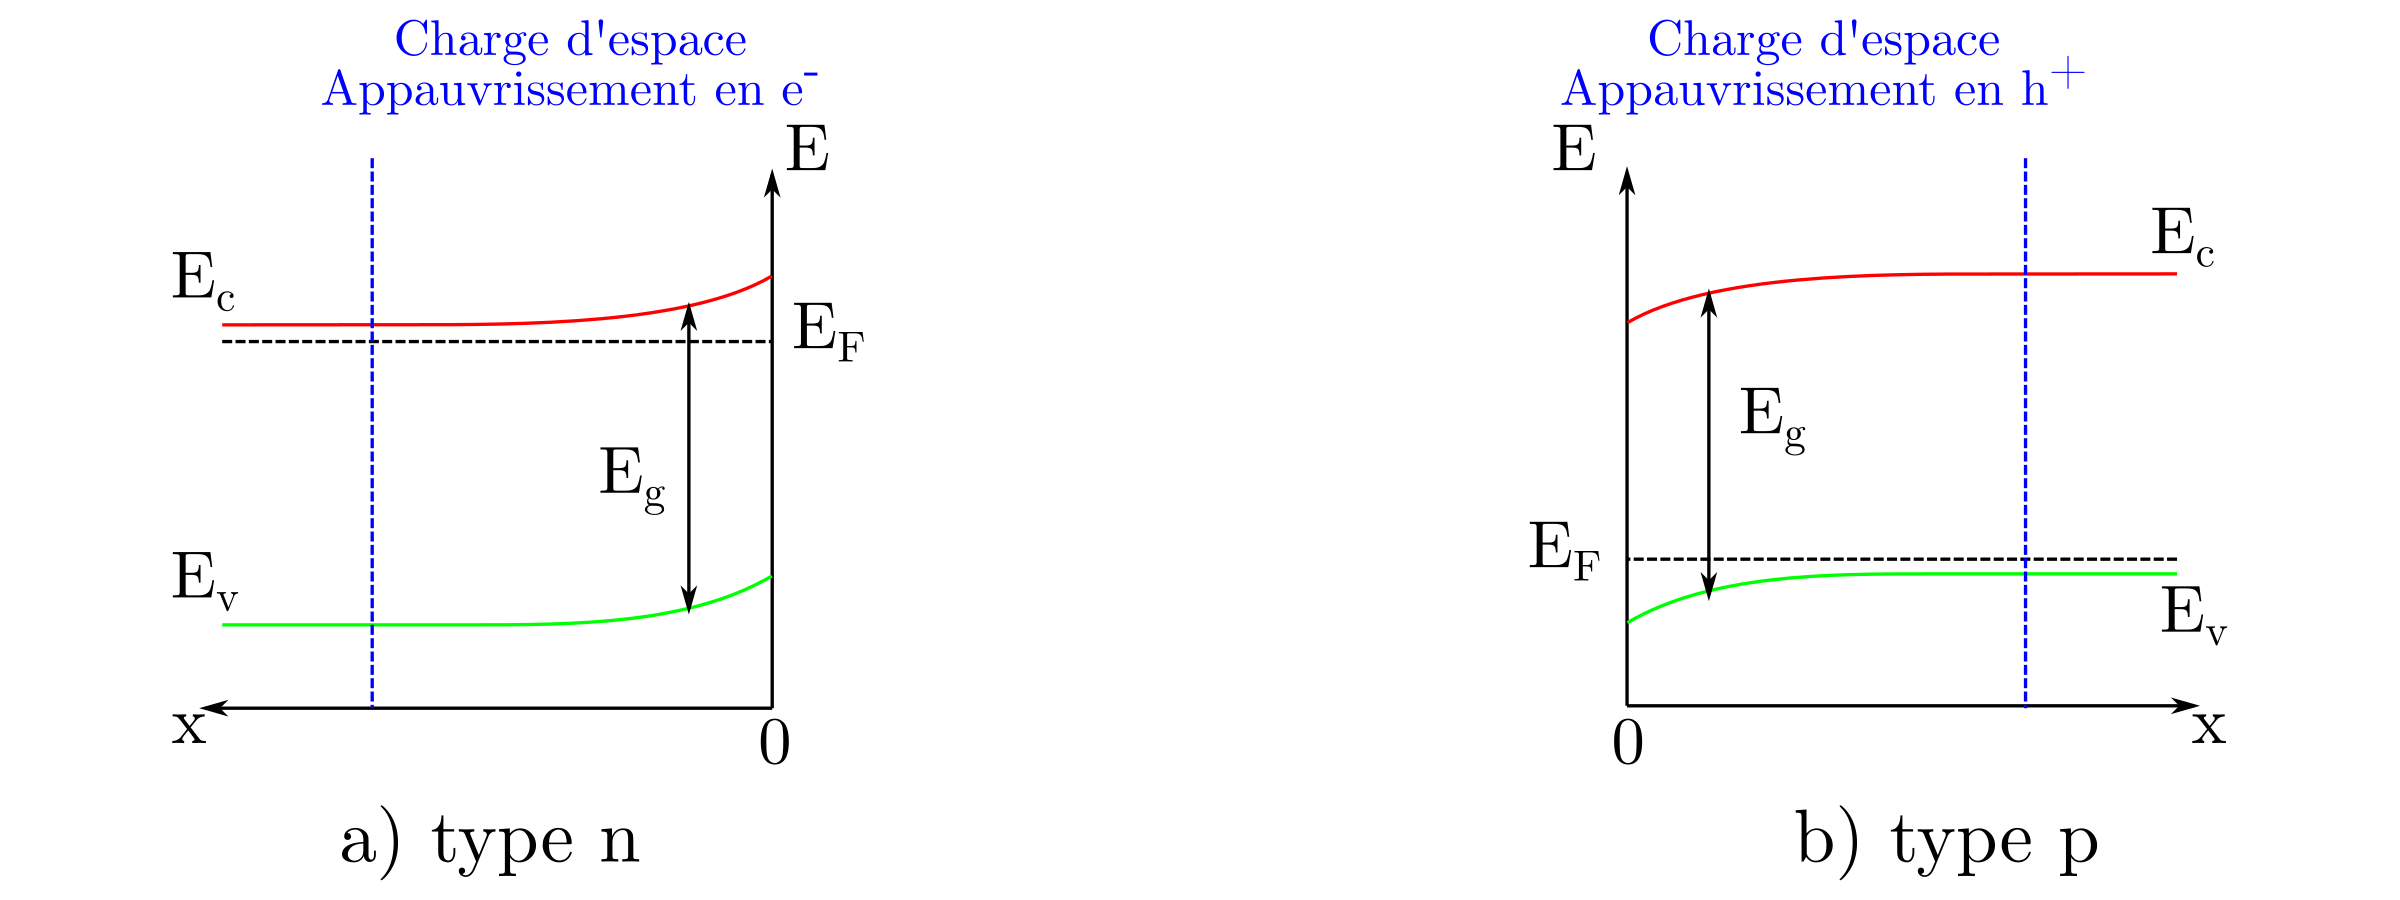
\includegraphics[width=0.85\textwidth]{Bending_Example.png}
        \caption[Représentation schématique d'une région de charge d'espace en situation d'appauvrissement en porteurs 
        de charge majoritaires pour un semiconducteur en contact avec un électrolyte: a)
        type \emph{n}, b) type \emph{p}.]
        {Représentation schématique d'une région de charge d'espace en situation d'appauvrissement en porteurs 
            de charge majoritaires pour un semiconducteur en contact avec un électrolyte (d'après \citet{Bard2002, Memming2008}): a)
        type \emph{n}, b) type \emph{p}.}
        \label{fig:bending_example}
    \end{figure}

    Les situations d'accumulation et d'appauvrissement et de bandes plates dans la région de charge d'espace
    peuvent être obtenues par polarisation du semiconducteur par rapport à une référence dans l'électrolyte. Si les
    hypothèses listées au début de ce paragraphe sont respectées, la polarisation ne modifie
    pas la position en énergie des bords de bande en surface, $\E_{cs}$ et $\E_{vs}$.
    La polarisation appliquée ne modifiera donc que les courbures de bande dans la région de charge d'espace.
    En fonction du potentiel appliqué (U) par rapport au potentiel correspondant à la situation de bandes plates
    ($U_{fb}$), trois situations différentes sont possibles (figure \ref{fig:bending_polarization}):

    \begin{itemize}
        \item U = $U_{fb}$: situation de bandes plates quel que soit le type de semiconducteur.
        \item U > $U_{fb}$: situation d'appauvrissement (accumulation) pour un semiconducteur de type \emph{n}
        (\emph{p}).
        \item U < $U_{fb}$: situation d'accumulation (appauvrissement) pour un semicondcuteur de type \emph{n}
        (\emph{p}).
    \end{itemize}

        
    \begin{figure}[H]
        \centering
        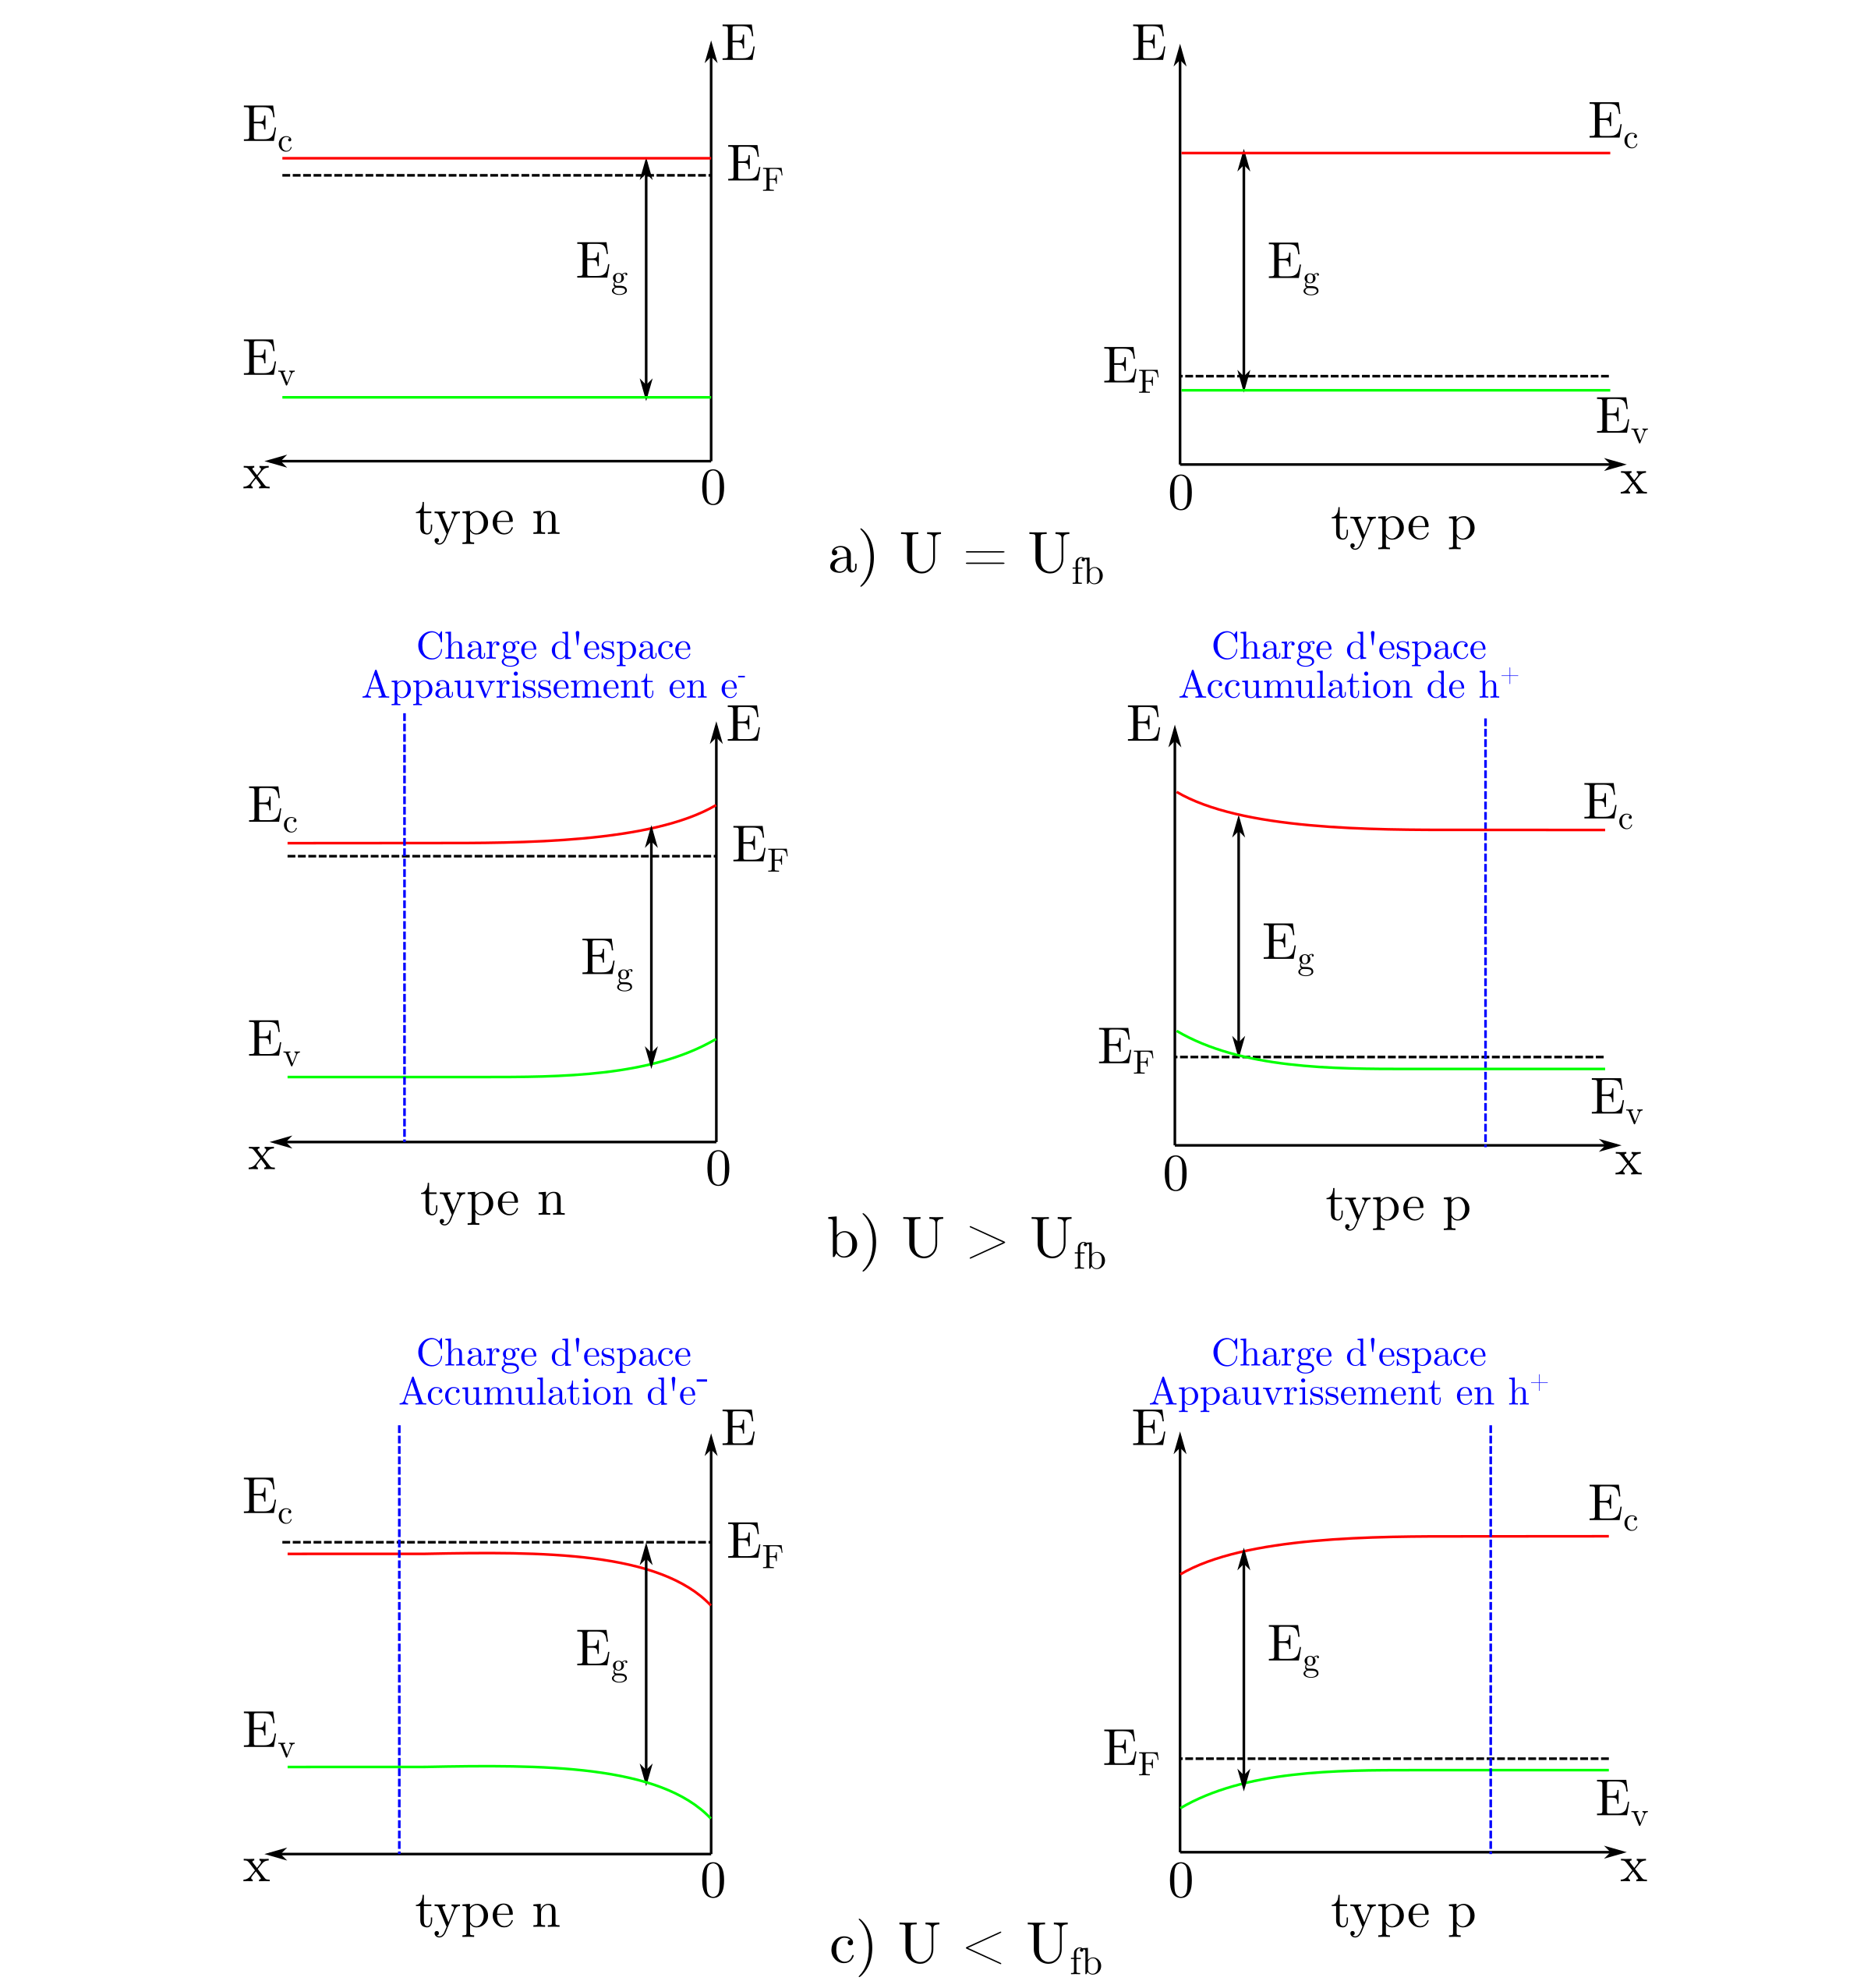
\includegraphics[width=0.85\textwidth]{Bending_Polarization.png}
        \caption[Représentation schématique des courbures de bandes pour des semiconducteurs de type \emph{n} et \emph{p}
        en contact avec un électrolyte en fonction de la polarisation appliquée: 
        a) U = $U_{fb}$,
        b) U > $U_{fb}$,
        c) U < $U_{fb}$.]
        {Représentation schématique des courbures de bandes pour des semiconducteurs de type \emph{n} et \emph{p}
            en contact avec un électrolyte en fonction de la polarisation appliquée (d'après \citet{Bard2002,
            Memming2008}): 
        a) U = $U_{fb}$, 
        b) U > $U_{fb}$, 
        c) U < $U_{fb}$.}
       \label{fig:bending_polarization}
    \end{figure}

    Sans illumination, des courants cathodiques (anodiques) vont être favorisés en situation d'accumulation d'électrons
    (trous) dans le cas d'un semiconducteur de type \emph{n} (\emph{p}). En effet, les porteurs de charge majoritaires
    d'un semiconducteur de type \emph{n} (\emph{p}) sont les électrons (trous). De manière réciproque, les courants
    anodiques (cathodiques) seront peu favorisés en situation d'appauvrissement dans le cas d'un semiconducteur de type
    \emph{n} (\emph{p}) puisque les trous (électrons) sont les porteurs de charge minoritaires. La jonction
    semiconducteur/électrolyte fonctionne comme une diode de Schottky.
             
    \subsubsection{Interface semiconducteur/électrolyte sous
    illumination}\label{subsec:semiconductor_electrolyte_contact_light}
     
    L'illumination d'une interface semiconducteur/électrolyte par des photons d'une énergie E ($h\nu$) supérieure
    au gap $\E_g$ génère des paires électron--trou dans le semiconducteur. En appliquant un potentiel adéquat,
    on peut séparer ces paires électron--trou de sorte que les 
    les porteurs de charge majoritaires soient évacués vers l'intérieur du semiconducteur alors que les
    porteurs de charge minoritaires rejoindront l'interface semiconducteur/électrolyte où ils pourront être transférer
    à une espèce redox présente dans
    l'électrolyte, générant un courant supplémentaire appelé \emph{photocourant}.

    La figure \ref{fig:photocurrent_generation} illustre de manière schématique le mécanisme de génération du photocourant.
    Pour un semiconducteur de type \emph{n} (\emph{p}), le photocourant est anodique (cathodique) puisque les électrons
    (trous) se dirigent vers le circuit externe alors que les trous (électrons) se dirigent vers l'interface externe. 
    Le photocourant devient donc significatif lorsque la jonction semiconducteur/électrolyte est en situation
    d'appauvrissement. Cela implique que le potentiel appliqué est supérieur (inférieur) au potentiel de bande plate
    dans le cas d'un semiconducteur de type \emph{n} (\emph{p}). 
    La figure \ref{subfig:ch1_Polarization_Curve-ntype} (\ref{subfig:ch1_Polarization_Curve-ptype}) illustre le
    photocourant anodique (cathodique) dans le cas d'un semiconducteur GaAs de type \emph{n} (\emph{p}).
    
    \begin{figure}[H]
        \centering
        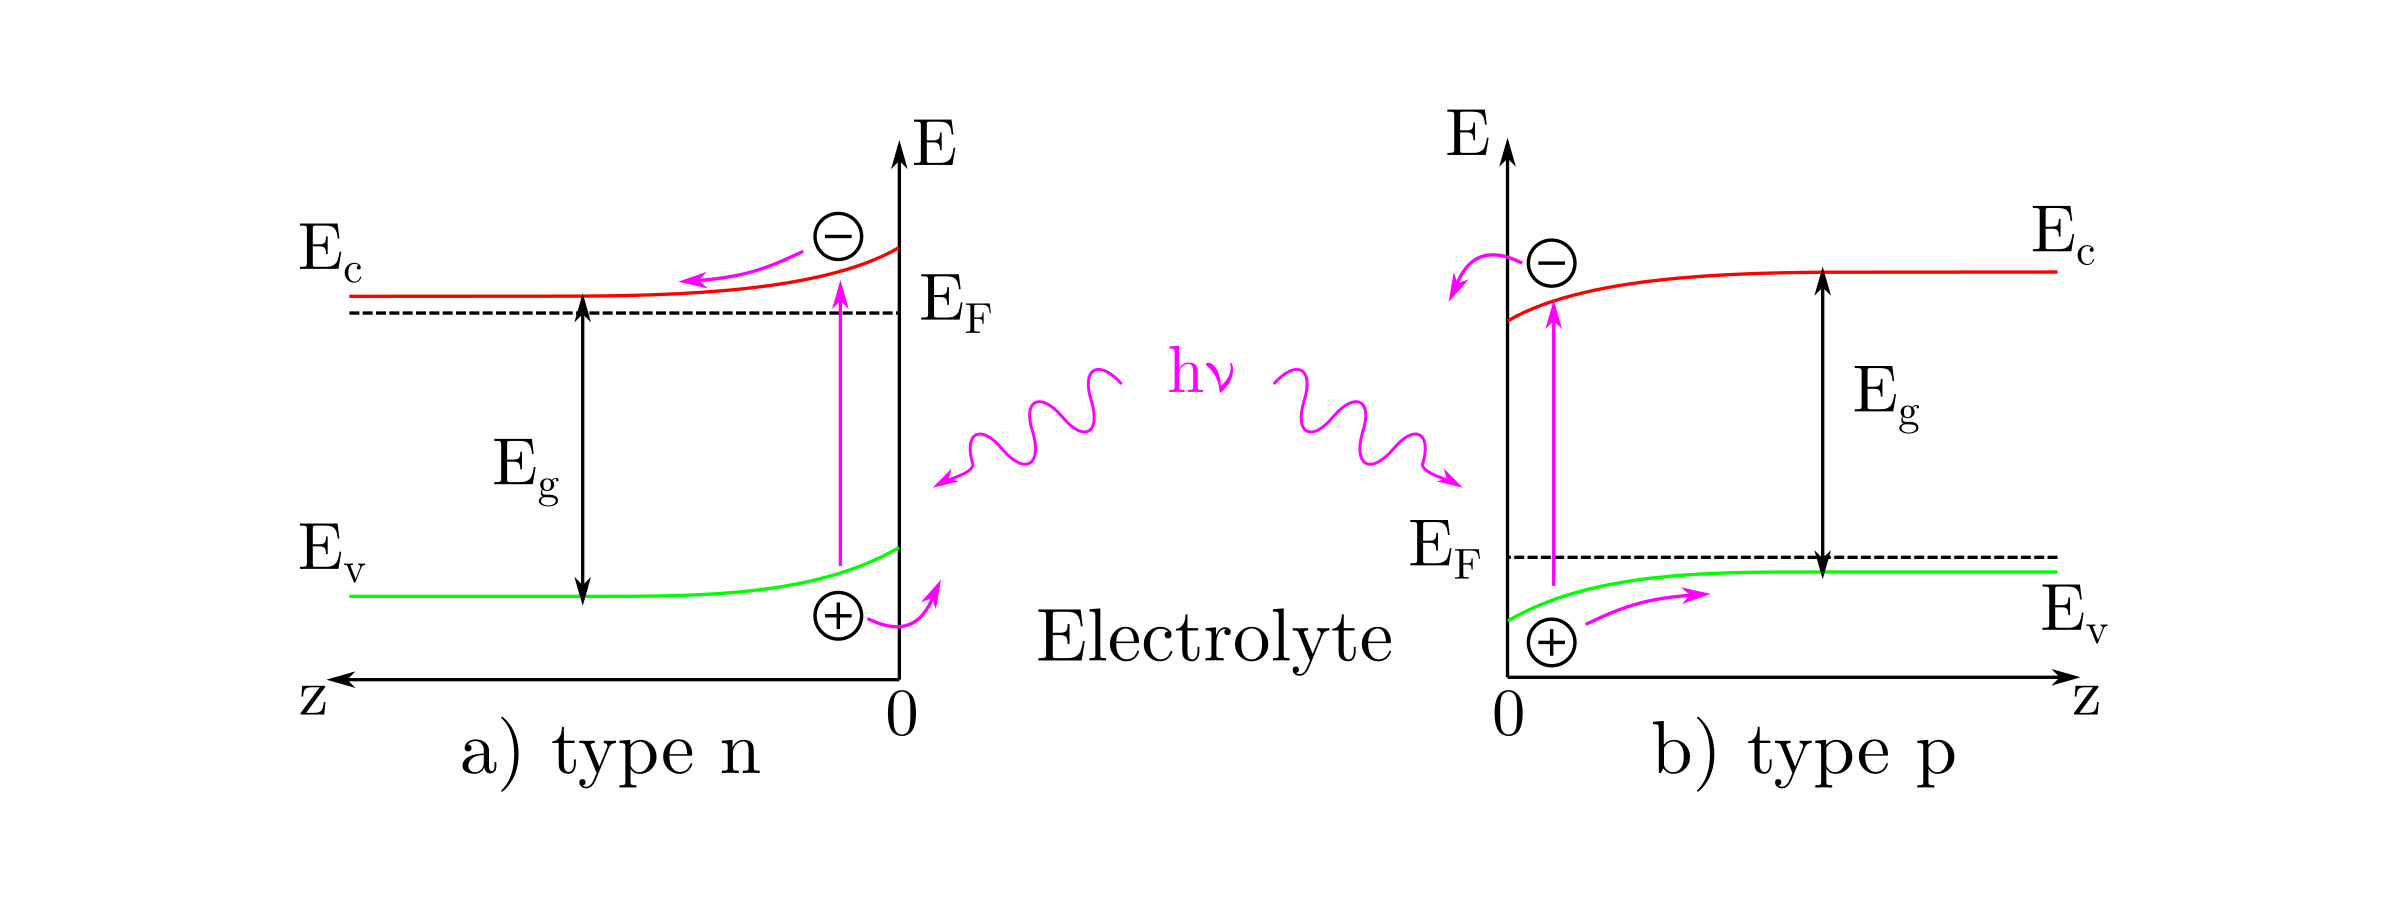
\includegraphics[width=0.85\textwidth]{Photocurrent_Generation.png}
        \caption[Représentation schématique du mécanisme de génération du photocourant.]
        {Représentation schématique du mécanisme de génération du photocourant (d'après \citet{Bard2002,
        Memming2008}).}
       \label{fig:photocurrent_generation}
    \end{figure}

    \begin{figure}[H]
        \centering
        \begin{subfigure}[b]{0.6\textwidth}
            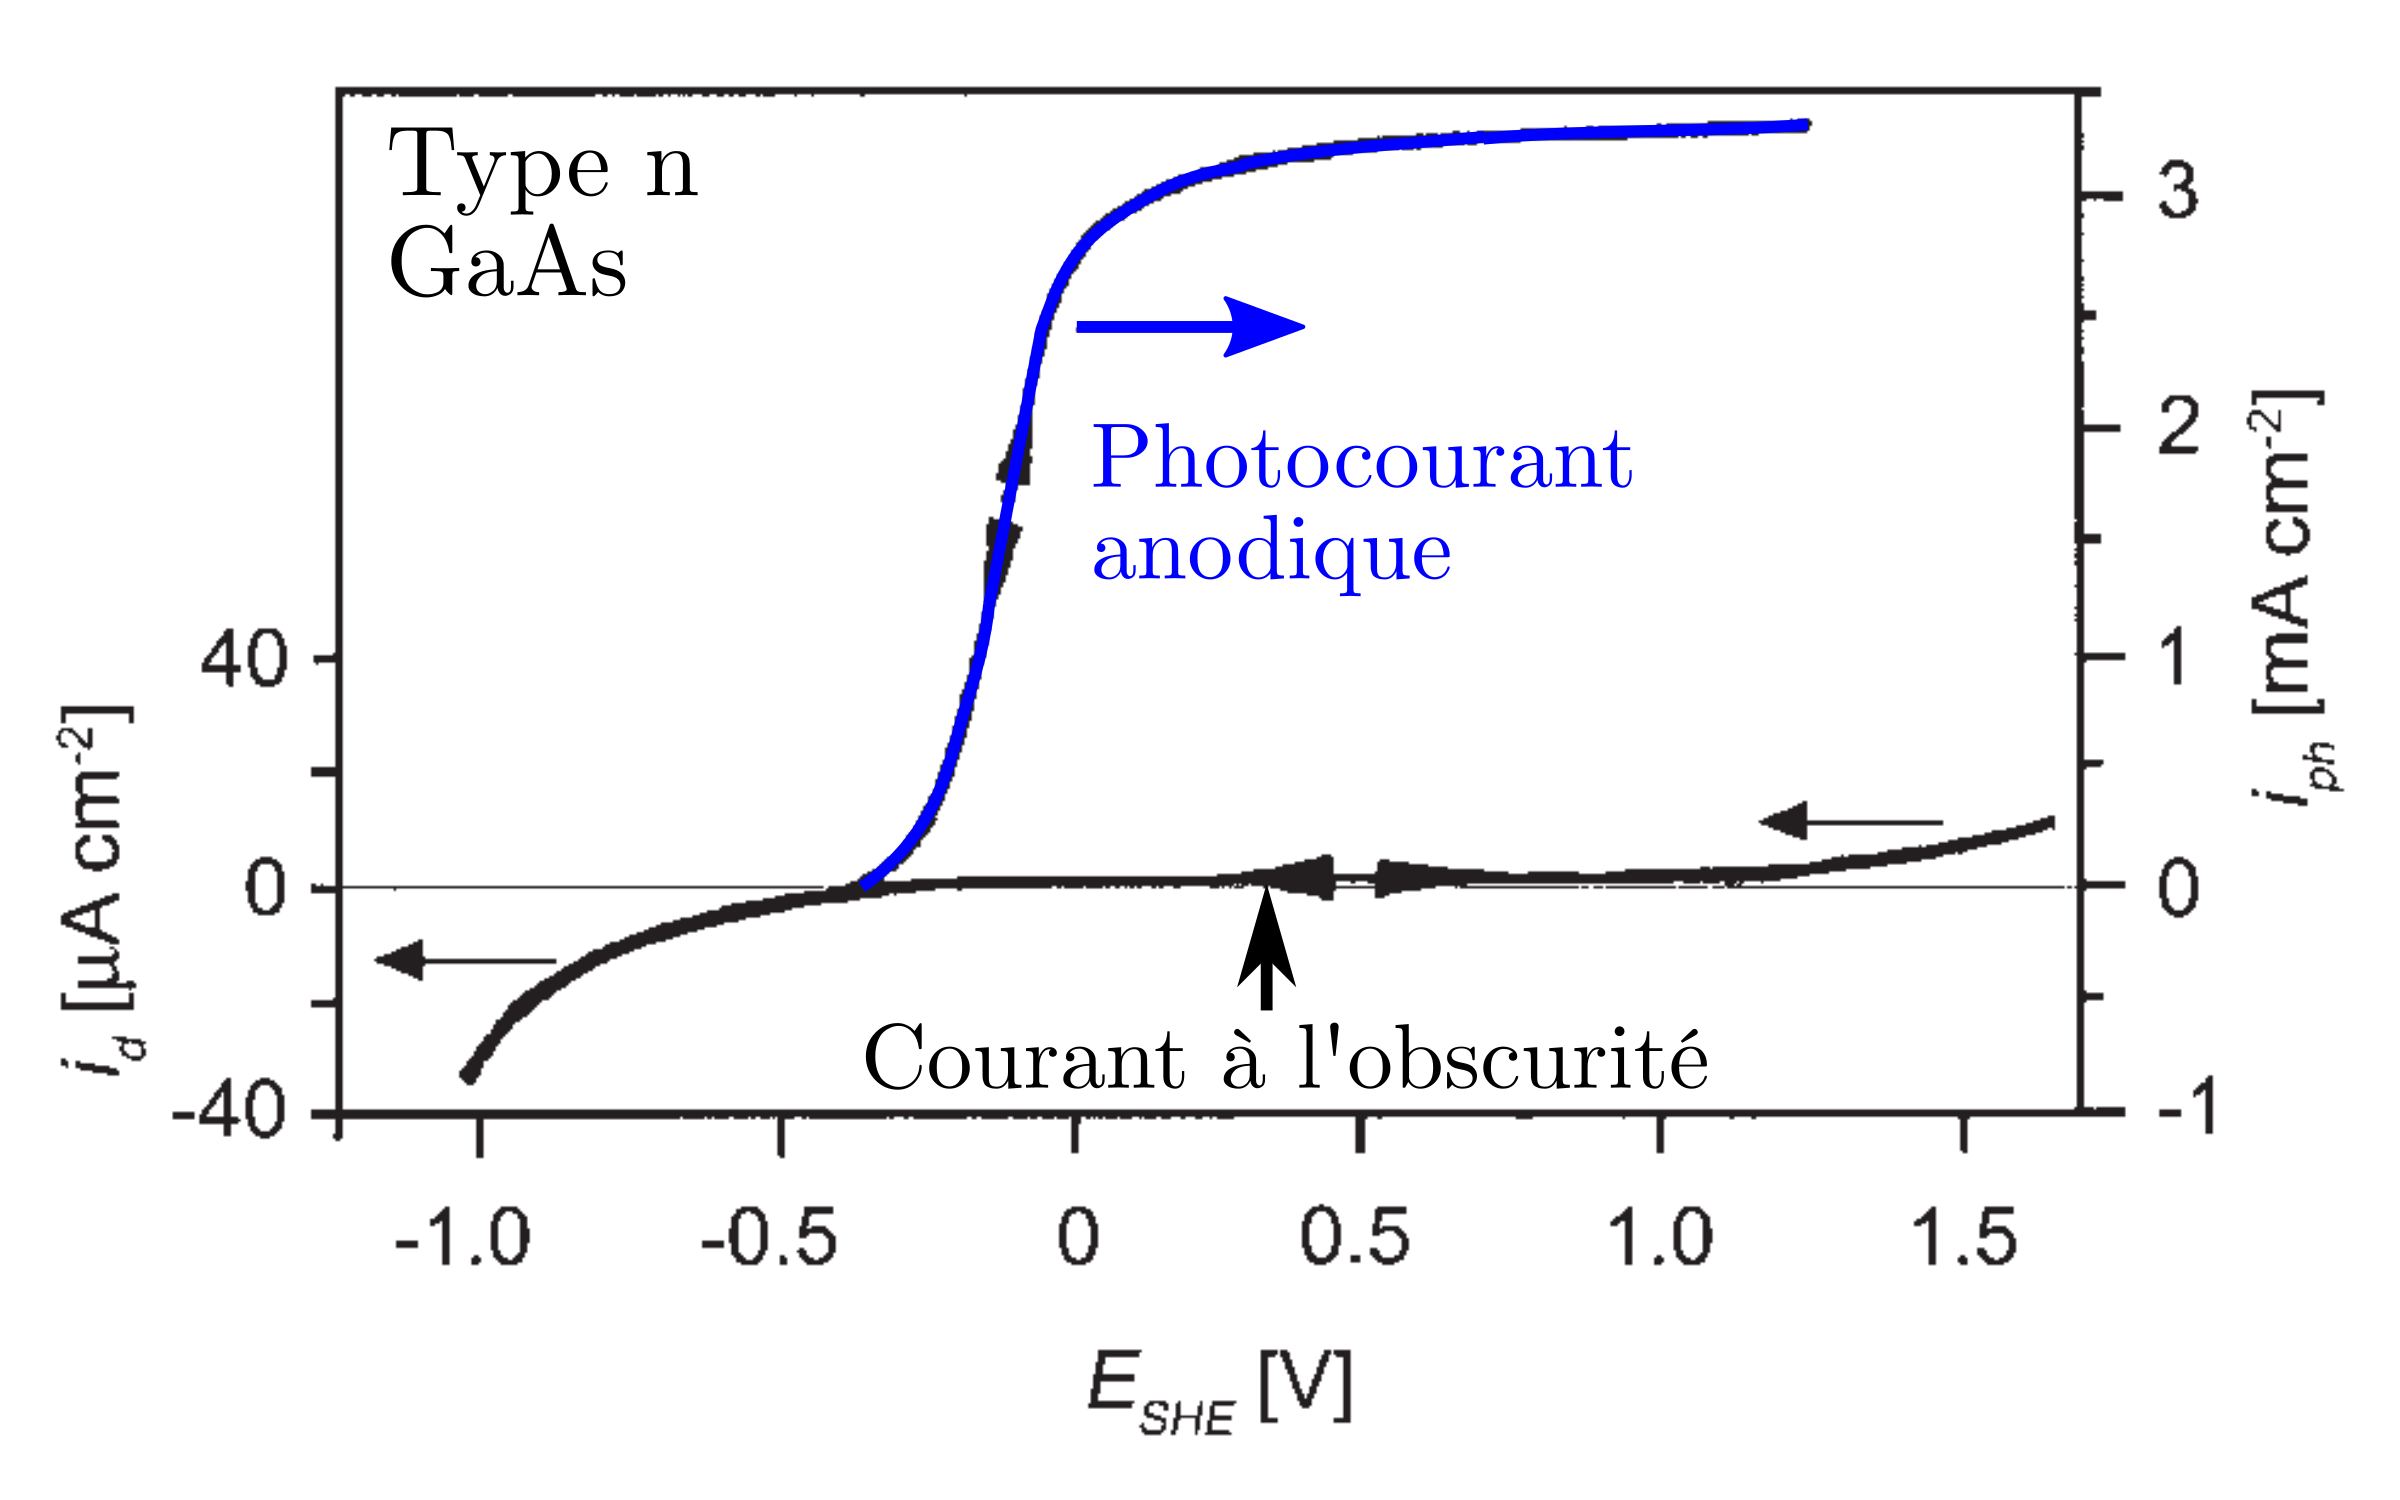
\includegraphics[width=\textwidth]{Iph_example_n_type.png}
            \caption{}
            \label{subfig:ch1_Polarization_Curve-ntype}
        \end{subfigure}

        \begin{subfigure}[b]{0.5\textwidth}
            \centering
            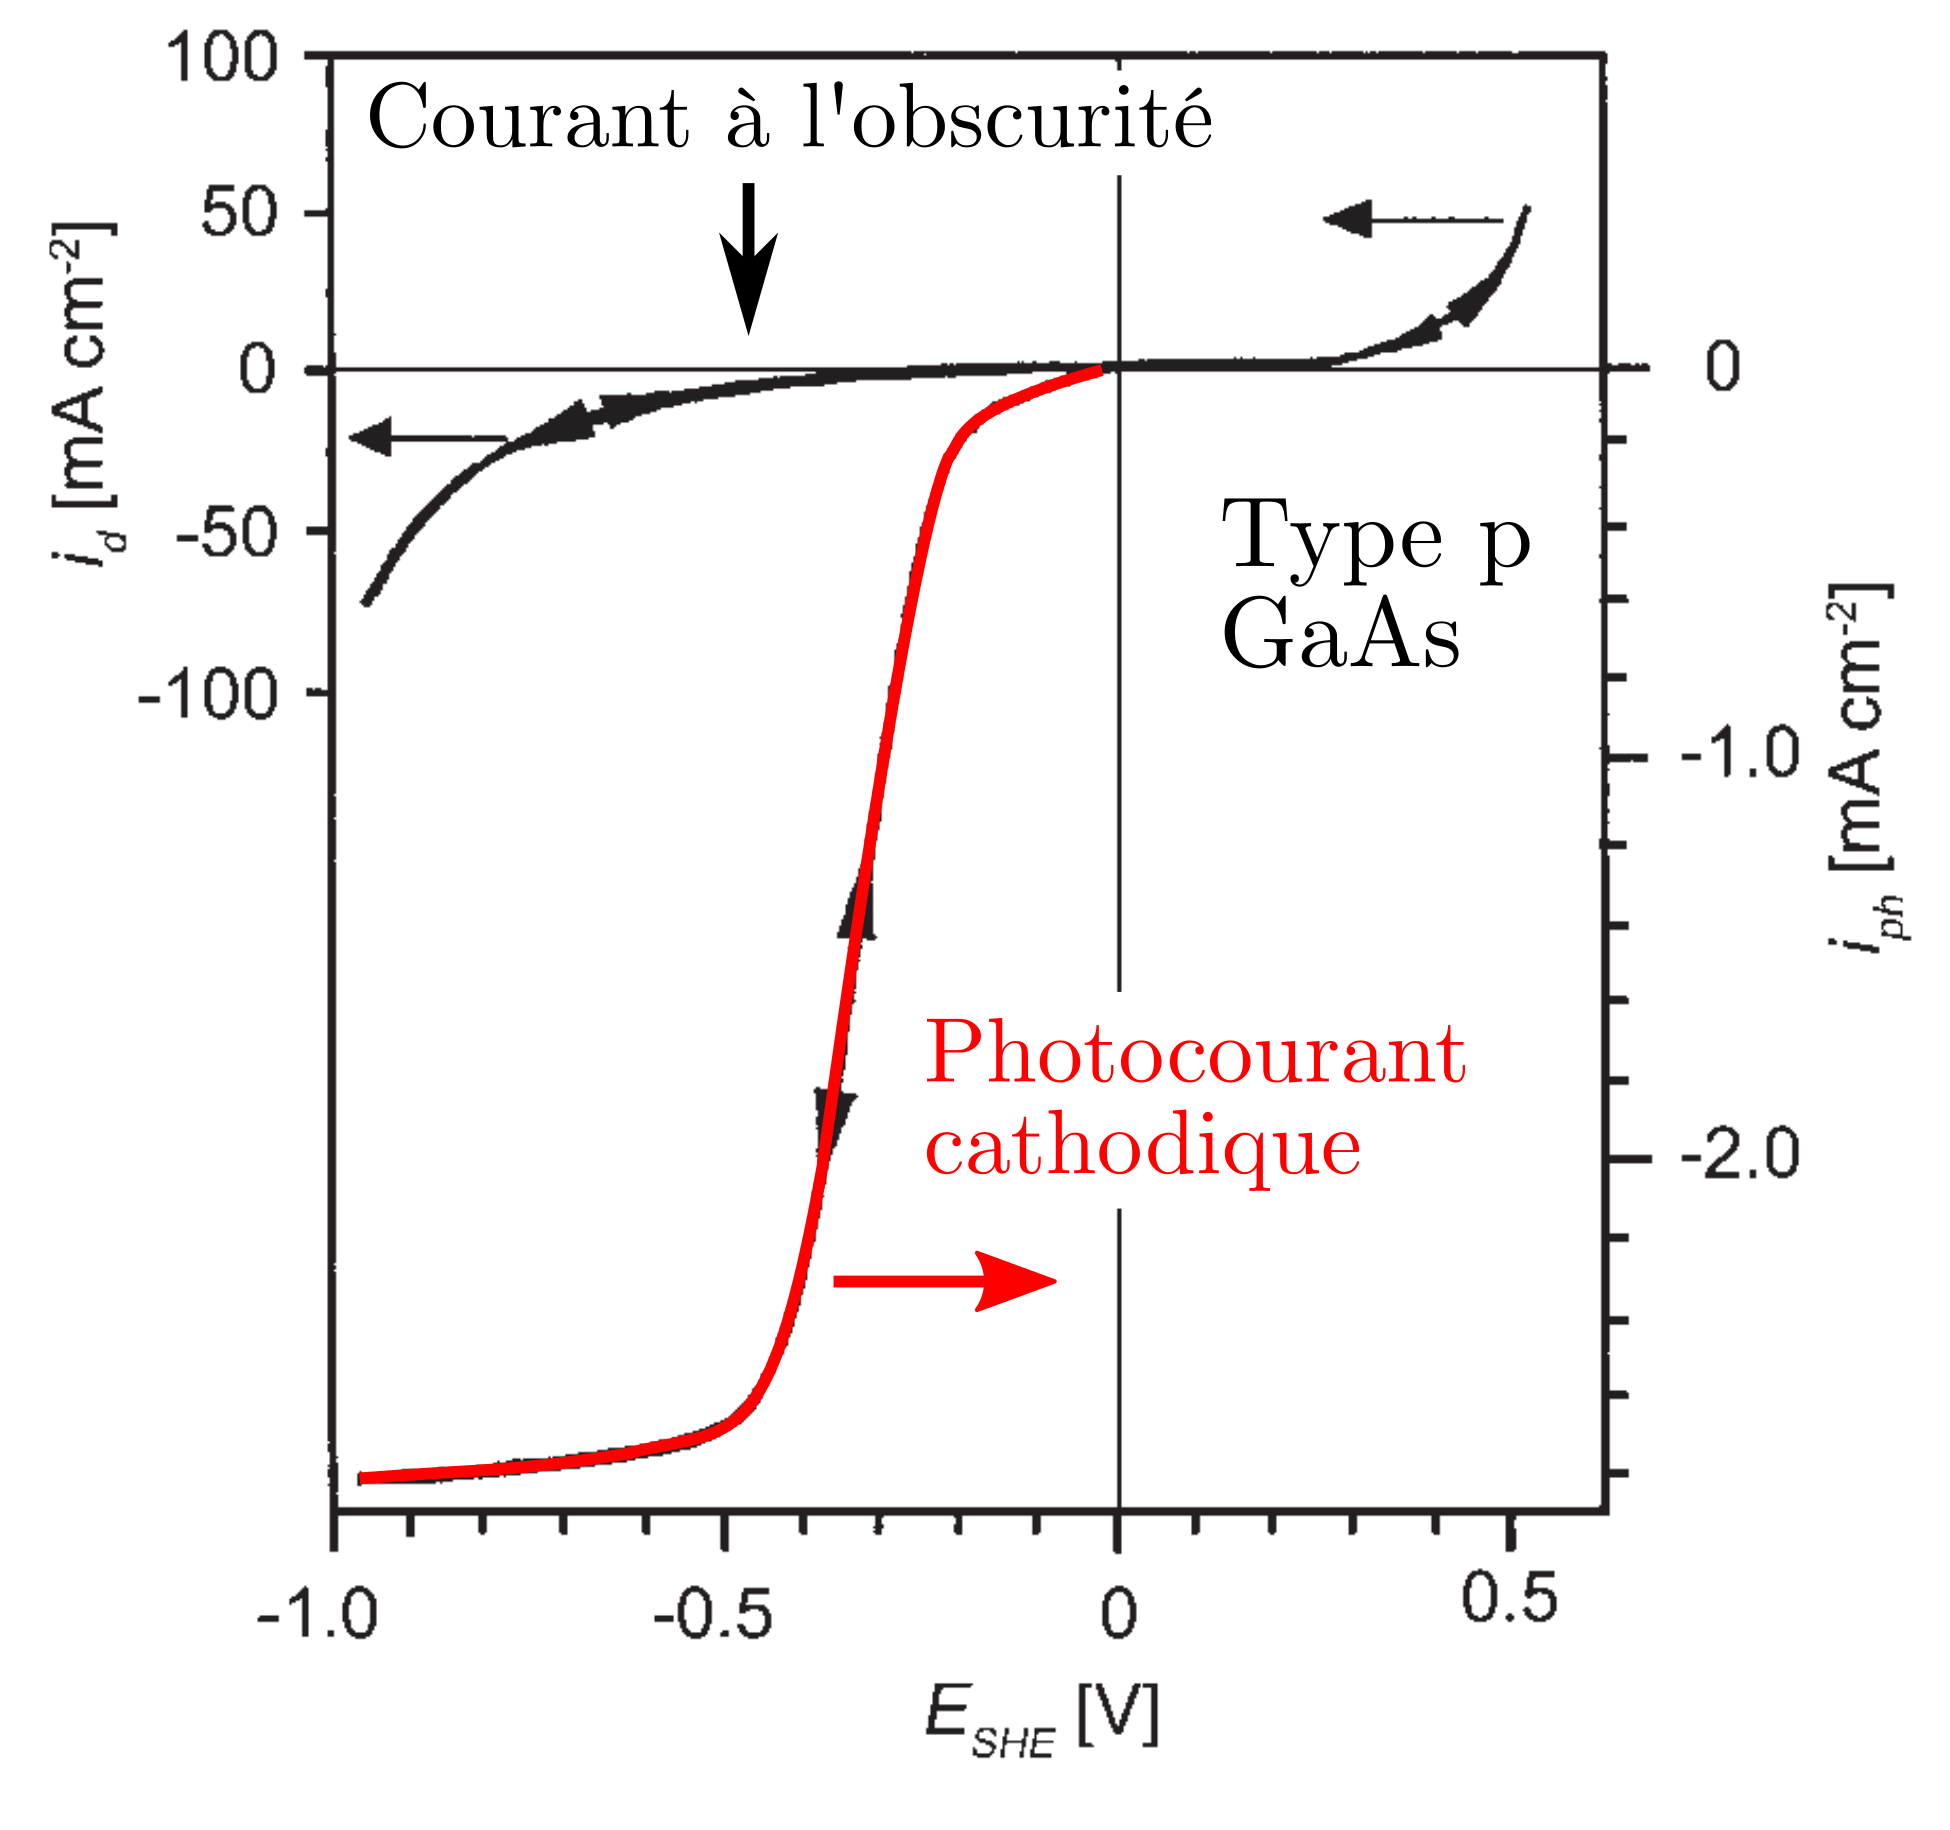
\includegraphics[width=\textwidth]{Iph_example_p_type.png}
            \caption{}
            \label{subfig:ch1_Polarization_Curve-ptype}
        \end{subfigure}
        \caption[Densité de photocourant $i_{ph}$ et densité de courant à l'obscurité $i_d$ en fonction du potentiel
            dans le cas du semiconducteur GaAs: 
            a) type \emph{n},
            b) type \emph{p}.]
        {Densité de photocourant $i_{ph}$ et densité de courant à l'obscurité $i_d$ en fonction du potentiel
            dans le cas du semiconducteur GaAs (d'après \citet{Plieth2008}): 
            a) type \emph{n},
            b) type \emph{p}.}
        \label{fig:ch1_photocurrent_examples}
    \end{figure}


    \citet{Gartner1959} et \citet{Butler1977} ont proposé un modèle, simple mais robuste, pour décrire le photocourant
    en faisant l'hypothèse que les paires électron--trou photogénérées dans la charge d'espace ne se recombinent pas. Le photocourant $\iph$
    est alors proportionnel au flux de photons incidents $\phi _0$. De plus, le photocourant dépend également du
    rapport relatif entre l'épaisseur de la charge d'espace $w_{\SC}$, la profondeur de pénétration des photons donnée
    par l'inverse du coefficient d'absorption $\alpha _{\SC}$ et de la longueur de diffusion moyenne des porteurs de
    charge minoritaires $L_{\cc}$. En d'autres termes, tous les
    photons absorbés dans une épaisseur égale à $w_{\SC} + L_{\cc}$ génèrent des paires électron--trou dont les porteurs de
    charge minoritaires sont transférés à l'électrolyte et par conséquent, participent au photocourant qui obéit donc à
    l'équation \ref{eq:iph_gartner_butler}. Lorsque $\alpha _{\SC} \cdot w_{\SC} \ll 1$ et $\alpha _{\SC} \cdot L_{\cc} \ll 1$, le photocourant peut être approximé par l'équation
    \ref{eq:iph_gartner_butler_simplified}.


    \begin{equation}
        I_{ph} = \phi _0 \left[ 1 - \frac{\exp (-\alpha _{\SC} \cdot w_{\SC})}{1+\alpha _{\SC} \cdot
        L_{\cc}} \right]
        \label{eq:iph_gartner_butler}
    \end{equation}

     \begin{equation}
        I_{ph} = \phi _0 \cdot \alpha _{\SC} \cdot w_{\SC}
        \label{eq:iph_gartner_butler_simplified}
    \end{equation}

    L'expression de l'épaisseur de la charge d'espace $w_{\SC}$, en situation d'appauvrissement, est donnée par
    l'équation \ref{eq:Space_charge_Schottky} dans le cadre de la théorie de Mott-Schottky. $N_{\cc}$ représente la
    concentration des porteurs de charge majoritaires, supposée égale au taux de dopage, $e$ correspond à la charge
    élémentaire de l'électron, U représente le potentiel appliqué à l'électrode, $U_{fb}$ représente le potentiel de
    bande plate, $\epsilon$ et $\epsilon _0$ représentent la permittivité relative du semiconducteur et la
    permittivité du vide, respectivement.
    
    \begin{equation}
        w_{\SC} = \sqrt{ \frac{2\epsilon \epsilon _0}{e N_{\cc}} (U-U_{fb}-\frac{kT}{e}) }
        \label{eq:Space_charge_Schottky}
    \end{equation}

    L'expression la plus utilisée du coefficient d'absorption $\alpha _{\SC}$ en fonction de l'énergie
    $h\nu$ des photons incidents est donnée par l'équation \ref{eq:absorption_coef}. La valeur de n dépend du type
    de transition bande--bande. Lorsque les transitions permises sont \emph{directes}, n vaut 0.5 alors que dans le cas des
    transitions \emph{indirectes}, n vaut 2.

    \begin{equation}
        \alpha _{\SC} = const \frac{(h\nu - \E_g)^n}{h\nu}
        \label{eq:absorption_coef}
    \end{equation}

    
    La dépendance en potentiel et en énergie du photocourant $\iph$ est donnée par l'équation
    \ref{eq:iph_substitute_W_alpha}. Cette
    dernière est obtenue en substituant l'épaisseur de la charge d'espace
    $w_{\SC}$ et le coefficient d'absorption $\alpha _{\SC}$ de l'équation \ref{eq:iph_gartner_butler_simplified} par
    les  équations \ref{eq:Space_charge_Schottky} et \ref{eq:absorption_coef}, respectivement.
             
     \begin{equation}
        I_{ph} = \phi _0 \cdot const \frac{(h\nu - \E_g)^n}{h\nu}
         \cdot \sqrt{ \frac{2\epsilon \epsilon _0}{e N_{\cc}} (U-U_{fb}-\frac{kT}{e}) }
        \label{eq:iph_substitute_W_alpha}
    \end{equation}

    A potentiel constant, la \emph{transformée linéaire} en énergie de l'équation
    \ref{eq:iph_substitute_W_alpha} est donnée par l'équation \ref{eq:iph_linear_transform}. A énergie constante, la \emph{transformée linéaire} en potentiel
    de l'équation \ref{eq:iph_substitute_W_alpha} est donnée par l'équation \ref{eq:iph_linear_transform_potential}.
    La transformée linéaire en énergie est utilisée pour déterminer des gaps (nous y reviendrons plus tard) alors que la
    transformée linéaire en potentiel est utilisée pour déterminer le type de semiconduction ainsi que les
    potentiels de bande plate.
    
    \begin{equation}
        \left[ \frac{I_{ph} \cdot h\nu}{\phi _0} \right] ^{1/n} = const \cdot (h\nu - \E_g)
        \label{eq:iph_linear_transform}
    \end{equation}

     \begin{equation}
        I_{ph}^2 = const \cdot (U-U_{fb}-\frac{kT}{e})
        \label{eq:iph_linear_transform_potential}
    \end{equation}

    
    \subsection[Exemples d'application de la photoélectrochimie]
    {Exemples d'application de la photoélectrochimie aux alliages de zirconium et aux alliages de
    nickel}\label{subsec:ch1_PEC_applications}

    \subsubsection{Identification des oxydes minoritaires}
     
    Les travaux de \citet{Benaboud2007} illustrent bien que la caractérisation photoélectrochimique se révèle être un outil
    performant pour mettre en évidence la présence d'oxydes
    mineurs dans la couche de zircone formée sur des échantillons de Zircaloy-4 par rapport à de la zircone formée sur du
    zirconium "pur". Les deux échantillons ont été oxydés en micro-thermobalance à \SI{470}{\degreeCelsius} avec une pression d'oxygène de
    \SI{150}{\milli\bar} pendant 1~h.
    
    Tout comme l'alliage Zircaloy-2, l'alliage Zircaloy-4 contient des éléments d'alliage (étain, fer, chrome) 
    se trouvant sous forme de précipités
    dans le métal. Lors de l'oxydation, ces éléments d'alliage se retrouvent dans la couche de zircone qui se forme à la
    surface et peuvent potentiellement être oxydés.
    Ces précipités oxydés sont des phases d'oxyde minoritaires dans la couche de zircone.
    En revanche la zircone qui se forme sur le zirconium "pur" ne devrait pas contenir de phases minoritaires. 
    En pratique, le zirconium "pur" contient des traces impuretés (fer et chrome) mais dont les concentrations sont bien
    plus faibles
    (environ dix fois moins de fer et environ cinq fois moins de chrome) que dans le cas de l'alliage Zircaloy-4.
    
    La figure \ref{subfig:benaboud_fig4} présente les spectres en énergie de photocourants mesurés sur l'alliage
    Zircaloy-4 et le zirconium "pur" où le fort photocourant observé à 5~eV, pour le Zircaloy-4 et le zirconium "pur",
    est une signature de l'oxyde majoritaire en l'occurrence la zircone monoclinique.
    Les photocourants mesurés sur les deux échantillons ne sont pas nuls aux basses énergies (<5~eV) mais leurs amplitudes 
    ne sont pas identiques, comme on peut l'observer en figure \ref{subfig:benaboud_fig5}.
    Ces photocourants mesurés à basse énergie sont des signatures des oxydes mineurs provenant des précipités oxydés.
    Malgré des concentrations en fer et chrome moins élevées dans l'échantillon de zirconium "pur", la caractérisation
    photoélectrochimique est suffisamment sensible pour détecter la présence de ces oxydes mineurs. 
   
    Les ruptures de pentes observées sur les spectres en énergie de photocourants permettent d'avoir une estimation des gaps des oxydes
    mineurs et de les identifier en s'appuyant sur les données de la littérature.
    Ainsi, l'auteur
    identifie de l'hématite $Fe_2O_3$, de la chromine $Cr_2O_3$ et une solution solide $(Fe_xCr_{1-x})_2O_3$.


    \begin{figure}[H]
        \centering
        \begin{subfigure}[b]{0.65\textwidth}
            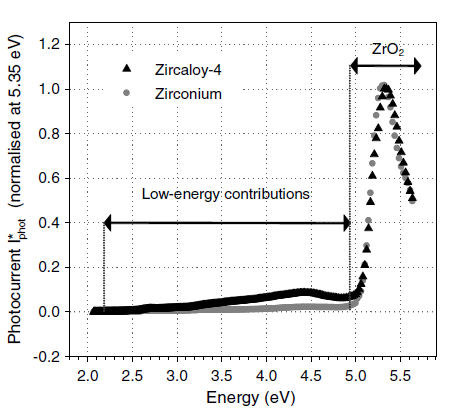
\includegraphics[width=\textwidth]{Benaboud2007-Fig4.png}
            \caption{}
            \label{subfig:benaboud_fig4}
        \end{subfigure}
        \begin{subfigure}[b]{0.65\textwidth}
            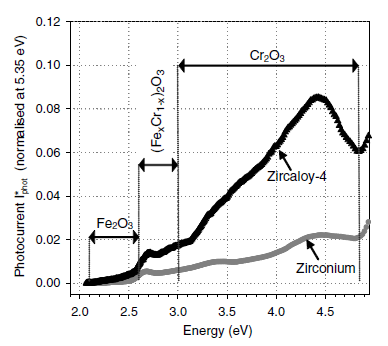
\includegraphics[width=\textwidth]{Benaboud2007-Fig5.png}
            \caption{}
            \label{subfig:benaboud_fig5}
        \end{subfigure}
        \caption[Spectres en énergie de photocourants mesurés sur des couches de zircone, sur un alliage
            Zircaloy-4 et sur 
            zirconium pur, formées à \SI{470}{\degreeCelsius} dans une atmosphère d'oxygène pendant 1~h:
            a) spectre complet de 2 à 5~eV, 
            b) zoom sur les contributions des oxydes mineurs.]
        {Spectres en énergie de photocourants mesurés sur des couches de zircone, sur un alliage Zircaloy-4 et sur 
            zirconium pur, formées à \SI{470}{\degreeCelsius} dans une atmosphère d'oxygène pendant 1~h \citep{Benaboud2007}:
            a) spectre complet de 2 à 5~eV, 
            b) zoom sur les contributions des oxydes mineurs.}
        \label{fig:benaboud_application}
    \end{figure}

    \subsubsection{Identification du type de semiconduction}

    Les travaux de \citet{Loucif2013} illustrent le changement de type de semiconduction des couches d'oxyde formées 
    sur des alliages de nickel oxydés en
    milieu primaire REP simulé pendant 500~h en fonction de la pression d'hydrogène (6.5 et \SI{0.05}{\bar}).
    La figure \ref{fig:loucif_application} présente les photocaractéristiques en potentiel mesurées pour différentes
    énergies dont les photocourants ont été normalisés à 1 à leur valeur maximale.
    
    A forte pression partielle d'hydrogène, la photocourant normalisé de la figure
    \ref{subfig:loucif_fig3_18} présente une forme en "V" suggérant un comportement isolant de la couche d'oxyde.
    En revanche, lorsque la pression partielle d'hydrogène est très faible, le photocourant normalisé de la figure \ref{subfig:loucif_fig3_19}
    augmente fortement lorsque le potentiel appliqué est de plus en plus anodique
    indiquant que la couche d'oxyde présente une semiconduction de type \emph{n}.
    
     \begin{figure}[H]
        \centering
        \begin{subfigure}[b]{0.48\textwidth}
            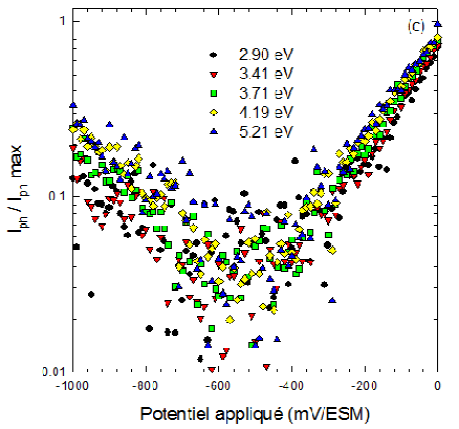
\includegraphics[width=\textwidth]{Loucif2012-Fig3-18.png}
            \caption{}
            \label{subfig:loucif_fig3_18}
        \end{subfigure}
        \begin{subfigure}[b]{0.48\textwidth}
            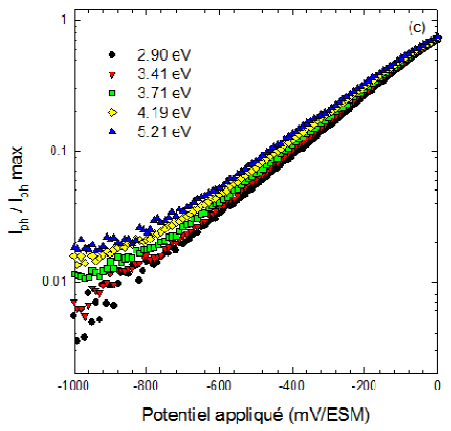
\includegraphics[width=\textwidth]{Loucif2012-Fig3-19.png}
            \caption{}
            \label{subfig:loucif_fig3_19}
        \end{subfigure}
        \caption[Photocaractéristique en potentiel de l'alliage 600 poli diamant et oxydé en milieu primaire REP simulé pendant
        500~h:
        a) $P_{H_2} = \SI{6.5}{\bar}$,
        b) $P_{H_2} = \SI{0.05}{\bar}$.]
        {Photocaractéristique en potentiel de l'alliage 600 poli diamant et oxydé en milieu primaire REP simulé pendant
            500~h \citep{Loucif2013}: 
        a) $P_{H_2} = \SI{6.5}{\bar}$,
        b) $P_{H_2} = \SI{0.05}{\bar}$.}
        \label{fig:loucif_application}
    \end{figure}

    Comme la majorité des caractérisations photoélectrochimiques, les deux exemples cités ci-dessus sont des
    caractérisations réalisées à température ambiante dans des cellules électrochimiques en verre.
    Réaliser des caractérisations photoélectrochimiques à haute température nécessite l'utilisation de cellules
    électrochimiques métalliques possédant un hublot pouvant laisser passer la lumière.
    \citet{Bojinov2002} ont montré la faisabilité à haute température sur des couches d'oxyde formées sur du
    fer pur. La figure \ref{subfig:Bojinov_HT_cell} illustre la cellule conçue pour travailler à
    haute température qui a permis d'obtenir des photocaractéristiques en énergie de la figure
    \ref{subfig:Bojinov_PEC_result}. Toutefois, la température a été limitée à \SI{200}{\degreeCelsius} et l'interval
    de travail en énergie a été limitée entre 1.8 et \SI{4}{\electronvolt}. A notre connaissance, cette étude est la
    seule dans le domaine de la photoélectrochimie à haute température.

	\begin{figure}[H] 
 		\centering 
            \begin{subfigure}[b]{0.55\textwidth}
                \includegraphics[width=\textwidth]{Bojinov_2002_Fig5b-redraw.png} 
                \caption{}
                \label{subfig:Bojinov_HT_cell}
            \end{subfigure}
            \quad
            \begin{subfigure}[b]{0.55\textwidth} 
                \includegraphics[width=\textwidth]{Bojinov_2002_Fig1.png} 
                \caption{}
                \label{subfig:Bojinov_PEC_result} 
           \end{subfigure}
       \caption[a) Spectres en énergie de photocourants à différentes températures mesurés sur des oxydes de fer
           (\SI{<200}{\degreeCelsius}, \SI{100}{\bar}),
                b) aperçu de la cellule de caractérisation photoélectrochimique.]
       {a) Spectres en énergie de photocourants à différentes températures mesurés sur des oxydes de fer
           (\SI{<200}{\degreeCelsius}, \SI{100}{\bar}),
       b) aperçu de la cellule de caractérisation photoélectrochimique \citep{Bojinov2002}.}
      \label{fig:HT_PEC_bojinov}
 	\end{figure}

%%%%%%%%%%%%%%%%%%%%%%%%%%%%%%%%%%%%%%%%%%%%%%%%%%%%%%%%%%%%%%%%%%%%%%%%%%%%%%%%%%%%%
%%%%%%%%%%%%%%%%%%%%%%%%%%%%%%%%%%%%%%%%%%%%%%%%%%%%%%%%%%%%%%%%%%%%%%%%%%%%%%%%%%%%%
\section{Conclusions}\label{sec:impacting_parameters}

    L'état de l'art exposé dans ce chapitre suggère que le phénomène de Shadow Corrosion résulte très
    probablement de la combinaison de quatre facteurs 
    liés au fonctionnement des REB: \emph{irradiation}, \emph{chimie de l’eau}, \emph{nature des matériaux} et la
    \emph{couplage galvanique} avec d’autres matériaux comme nous tentons de le schématiser en
    figure \ref{fig:impacting_parameters} où les principaux facteurs sont symbolisés par des cercles et les paramètres
    d'intérêt pour l'étude expérimentale sont symbolisés par des rectangles. 

    \begin{figure}[H] 
 		\centering 
 		\includegraphics[width=0.95\textwidth]{Impacting_Parameters-3.png} 
 		\caption{Principaux facteurs d'influence de la Shadow Corrosion et les paramètres d'intérêt pour son étude
        expérimentale.} 
 		\label{fig:impacting_parameters} 
 	\end{figure}

    Comme vu plus haut, l’irradiation que subissent les matériaux englobe des rayonnements électromagnétiques allant 
    des UV aux
    rayonnements $\gamma$ ainsi que le rayonnement neutronique. Ces rayonnements peuvent impacter le transport ionique
    ainsi que le transport électronique dans les oxydes formés sur les gaines de confinement et les grilles de maintien. 
    La principale conséquence de l'irradiation est selon nous la perturbation de l'équilibre qui s'établit entre le transport
    ionique et le transport électronique afin d'assurer l'électroneutralité dans la couche de zircone.
    %Toutefois, il
    %semble y avoir peu de preuves avérées sur le lien direct entre l’accélération de la cinétique de corrosion et 
    %l’augmentation des coefficients de diffusion de l’oxygène dans la couche de zircone.

    Etudier l'impact du rayonnement neutronique et du rayonnement $\gamma$ nécessite des moyens expérimentaux
    conséquents. En revanche, l'illumination avec de la lumière UV semble être un moyen plus accessible 
    permettant de tenter de simuler
    une partie de l'effet de l'irradiation, à condition de disposer d'un flux non négligeable de photons y compris
    pour ceux ayant une énergie
    supérieure au gap de la zircone monoclinique soit \SI{5}{\electronvolt}.

    Nous avons également vu que la radiolyse de l’eau crée des espèces radicalaires ayant un pouvoir oxydant élevé. La
    recombinaison de ces espèces produit principalement du peroxyde d’hydrogène, qui augmente le
    pouvoir oxydant de l'électrolyte et peut potentiellement entraîner une dissolution partielle de la zircone. 
    Des injections en continu de péroxyde d'hydrogène dans l'électrolyte pourront permettre de simuler l'effet chimique
    de la radiolyse. 
    
    Les éléments fer, nickel et chrome, provenant de la dissolution des phases intermétalliques 
    peuvent doper la couche de zircone et ainsi modifier le comportement électrochimique global des alliages Zy2.
    De plus, ces mêmes éléments peuvent être présents dans l'électrolyte et sont susceptibles de modifier le
    comportement électrochimique global du Zy2 et de l'Inconel 718.
    Même si le lien entre la présence de cations dans
    l'électrolyte et l'accélération de la corrosion des alliages de zirconium n'est pas clairement établi, il sera
    possible de modifier la chimie de l'électrolyte pour examiner l'influence de ces cations sur le comportement
    électrochimique des alliages.
   
    Les méthodes électrochimiques classiques semblent bien être adaptée à l'étude des comportements
    électrochimiques des matériaux dans le cadre du mécanisme de couplage galvanique proposé par \citet{Lysell2004} et
    également modélisé par \citet{Buttin2011}.
    Nous nous axerons sur trois techniques: suivi du potentiels électrochimiques, suivi de courants de
    couplages et tracés de courbes de polarisation. Ces techniques seront présentées dans le
    chapitre 2.

    La technique de caractérisation photoélectrochimique (PEC) est moins communément utilisée mais est performante
    pour suivre les modifications subies par la couche d'oxydation en fonction des conditions expérimentales. 
    Afin de pouvoir réaliser des photocaractéristiques en énergie et/ou en potentiel à la température d'un réacteur à
    eau bouillante, soit
    \SI{280}{\degreeCelsius}, il a été nécessaire de développer une cellule électrochimique spécifique.
    Les étapes de conception, développement et de validation de l'installation développée seront décrites au chapitre
    \ref{chap:design}.
    Le chapitre 4 sera axé sur la présentations et la discussion des résultats de notre étude.

    % \ref{chap:ch4_results}
    \singlespacing
\printbibliography[heading=subbibintoc]
    \onehalfspacing
\end{refsection}

	
	% !TEX root=../../main_file.tex
% !TeX TS-program = pdflatex
% !TeX checkspelling = fr_toutesvariantes


\chapter{Matériaux et méthodes expérimentales}\label{chap:methods} 
%\chaptermark{Mat. et méth. électrochimiques}
\begin{refsection}
\minitoc

\section{Introduction}
Les principales caractéristiques des matériaux, sélectionnés pour l'étude du phénomène de Shadow Corrosion, 
sont décrites dans un premier temps. 
Dans un second temps, les conditions d'oxydation
en micro-autoclave sont détaillées avec au préalable une description de la manière dont a été simulé l'environnement REB en
termes de température, pression et chimie. Les limitations liées à l'utilisation des micro-autoclaves sont
également abordées.
Enfin, les méthodes électrochimiques classiques utilisées dans ce travail sont présentées avec quelques précisions sur les
difficultés de mesure liées à l'utilisation de cellules électrochimiques métalliques. La technique de mesure en
photoélectrochimie sera abordée au chapitre \ref{chap:design}.

%%%%%%%%%%%%%%%%%%%%%%%%%%%%%%%%%%%%%%%%%%%%%%%%%%%%
\section{Matériaux étudiés}\label{sec:ch2_materials}

    Le chapitre \ref{chap:ch1_bib} a montré que le principal alliage utilisé pour les gaines de confinement est l'alliage
    \emph{Zircaloy-2} alors que le principal alliage utilisé pour les grilles de maintien est l'alliage \emph{Inconel 718}. 
    L'ensemble de nos travaux expérimentaux a été réalisé avec ces alliages
    fournis par Cezus pour le \emph{Zircaloy-2} et Goodfellow pour l'\emph{Inconel 718}, respectivement. Dans la suite, ces deux
    alliages sont dénommés \emph{Zy2} et \emph{Inc718}.   
    
    Les deux alliages sont fournis sous forme de tôle industrielle ayant une épaisseur de \SI{2.96}{\milli\meter} et de
    \SI{1}{\milli\meter} pour Zy2 et Inc718, respectivement. Les compositions chimiques nominales de ces deux
    alliages sont données dans les tableaux \ref{tab:ch2_Zy2_composition} et \ref{tab:ch2_718_composition}. 

    \begin{table}[H]
    \centering
        \begin{tabular}{p{0.08\textwidth}%
                        p{0.081\textwidth}%
                        p{0.08\textwidth}%
                        p{0.08\textwidth}%
                        p{0.08\textwidth}%
                        p{0.08\textwidth}%
                        p{0.08\textwidth}%
                        p{0.09\textwidth}%
                        p{0.09\textwidth}}
            \toprule
            \textbf{Ref. \newline Cezus} & Zr & Sn & Fe & Cr & Ni & O (ppm) & Si (ppm) & C (ppm) \\\midrule
            810393 & Bal. & 1.32 & 0.169 & 0.108 & 0.055 & 1170 & 107 & 157 \\
            \bottomrule
        \end{tabular}

    \caption[Composition chimique de l'alliage Zy2.]
    {Composition chimique de l'alliage Zy2 exprimée en pourcentage massique sauf indication contraire.}
    \label{tab:ch2_Zy2_composition}
    \end{table}


    \begin{table}[H]
    \centering
        \begin{tabular}{p{0.2\textwidth}%
                        p{0.1\textwidth}%
                        p{0.1\textwidth}%
                        p{0.1\textwidth}%
                        p{0.1\textwidth}%
                        p{0.1\textwidth}%
                        p{0.1\textwidth}}
            \toprule
            \textbf{Ref. \newline Goodfellow} & Ni & Cr & Fe & Nb & Mo & Ti \\\midrule
            LS412242MKS & 53 & 19 & 19 & 5 &3 & 1 \\
            \bottomrule
        \end{tabular}

    \caption[Composition chimique de l'alliage Inc718.]
    {Composition chimique de l'alliage Inc718 exprimée en pourcentage massique.}
    \label{tab:ch2_718_composition}
    \end{table}

    Les
    différents échantillons de l'étude ont été prélevés sur ces tôles industrielles par une découpe fil. 
    L'état de surface initial des échantillons a consisté en un polissage au papier abrasif de grade P1200.

    La figure \ref{subfig:ch2_Zy2_microstructure_optical} montre la microstructure de l'alliage Zy2 observée au
    microscope optique en lumière polarisée. La taille de grain est d'environ une dizaine de microns. Les précipités
    sont distribués de manière homogène aux joints de grains et dans les grains comme on peut le constater sur le cliché MET de la
    figure \ref{subfig:ch2_Zy2_SPPs_MET}. La taille moyenne des précipités est de \SI{150}{\nano\meter}.

     Les échantillons Inc718 ont été traités thermiquement sous air afin de simuler le procédé de conditionnement des
    grilles de maintien avant leur mise en réacteur. Le traitement thermique effectué est schématisé en figure
    \ref{fig:ch2_thermal_treat}.
    L'oxyde formé lors du traitement thermique est ensuite éliminé par polissage au papier
    abrasif de grade P1200.

    \begin{figure}[H]
    \centering
        \begin{subfigure}[b]{0.5\textwidth}
            \includegraphics[width=\textwidth]{Guerin_2007-Fig2-redraw.png} 
			\caption{}
			\label{subfig:ch2_Zy2_microstructure_optical}
        \end{subfigure}
        \quad
        \begin{subfigure}[b]{0.4\textwidth}
            \includegraphics[width=\textwidth]{Guerin_2007-Fig10-redraw.png} 
			\caption{}
			\label{subfig:ch2_Zy2_SPPs_MET}
        \end{subfigure}
    \caption[Microstructure de l'alliage Zy2]
    {Microstructure de l'alliage Zy2: 
            a) cliché optique en lumière polarisée (X200),
            b) cliché MET \citep{Guerin2007}.}
    \label{fig:ch2_microstructure}
    \end{figure}    

    \begin{figure}[H]
        \centering
            \includegraphics[width=0.65\textwidth]{140778-ATT-X718.png}
        \caption{Traitement thermique appliqué aux échantillon de Inc718 pour simuler le procédé de conditionnement
        des grilles de maintien avant leur mise en réacteur.}
        \label{fig:ch2_thermal_treat}
    \end{figure}

    Trois géométries d'échantillons ont été utilisées, \emph{coupon rectangulaire}, \emph{disque} et \emph{anneau}, 
    dont les représentations schématiques sont
    fournies en figure \ref{fig:ch2_samples_schemes}. Les coupons rectangulaires ont
    seulement été utilisés en micro-autoclaves. En effet, cette géométrie est adaptée à la géométrie longiligne des
    micro-autoclave (\S\ref{sec:ch2_MA_oxydation}) et facilite la prise de contact pour les mesures
    électrochimiques (\S\ref{sec:ch2_electrochemistry}) grâce à la queue de contact en extrémité. 
    Les géométries disque et anneau ont été utilisées dans la cellule électrochimique haute température développée dans le cadre du présent travail
    de thèse. Le détail lié au choix de ces géométries seront abordés au chapitre \ref{chap:design}.

%    \begin{figure}[!htb]
%    \centering
%        \begin{subfigure}[b]{0.75\textwidth}
%            \includegraphics[width=\textwidth]{140778-Sample_Size-Coupons.png} 
%			\caption{}
%			\label{subfig:ch2_coupons_scheme}
%        \end{subfigure}
%        \quad
%        \begin{subfigure}[b]{0.15\textwidth}
%            \includegraphics[width=\textwidth]{140778-Sample_Size-Disc.png} 
%			\caption{}
%			\label{subfig:ch2_disc_scheme}
%        \end{subfigure}
%    \caption{Représentation schématique de la géométrie des échantillons: a) coupon, b) disque.}
%    \label{fig:ch2_samples_schemes}
%    \end{figure} 

    \begin{figure}[H]
        \centering
        \includegraphics[width=0.85\textwidth]{140778-Sample_Only.png}
        \caption{Représentation schématique de la géométrie des échantillons: a) coupon rectangulaire, b) disque, c)
        anneau.}
        \label{fig:ch2_samples_schemes}
    \end{figure}


%%%%%%%%%%%%%%%%%%%%%%%%%%%%%%%%%%%%%%%%%%%%%%%%%%%
\section{Simulation de l'environnement REB}\label{sec:ch2_T_P}

    Le tableau \ref{tab:operating_parameters_reactors} du chapitre \ref{chap:ch1_bib} montre que la température d'un
    réacteur à eau bouillante varie entre 272 et \SI{278}{\degreeCelsius} à l'entrée et entre 280 et
    \SI{300}{\degreeCelsius} à la sortie pour une pression comprise entre 70 et 80~bars. De plus, les réacteurs à
    eau bouillante sont des réacteurs diphasiques avec la présence de vapeur d'eau générée directement au niveau des
    gaines de confinement du combustible. 

    Le contrôle de l'ébullition au niveau des échantillons lors d'essais de corrosion en laboratoire n'est pas simple
    à obtenir. De plus, la présence d'ébullition ne facilite pas les mesures électrochimiques puisque les bulles de
    vapeur masquent une partie de la surface de l'échantillon et rendent difficile la normalisation des courants mesurés par
    rapport à la surface exposée.

    Afin de s'affranchir de ces potentiels problèmes expérimentaux liés à la présence de phase vapeur, il a été décidé de
    travailler en milieu monophasique. Par conséquent, le milieu REB a été simulé en fixant la température à sa valeur
    basse de sortie, soit \SI{280}{\degreeCelsius}, sous une pression de \SI{80}{\bar}.

    L'électrolyte utilisé ici pour simuler le milieu REB est de l'eau ultra-pure 
    dans laquelle on peut faire varier la teneur en oxygène dissous ainsi que la
    concentration en autres composés chimiques. 
    La manière dont la teneur en oxygène dissous a été contrôlée finement sera abordée au chapitre \ref{chap:design}.
    Le
    détail des compositions chimiques des électrolytes utilisées pour nos expériences sera donné au cours de l'exposé
    des résultats au chapitre 4.
    %\ref{chap:ch4_results}.

    Il convient de rappeler ici que l'eau ultra-pure présente une faible conductivité de l'ordre de 
    \SI{0.06}{\micro\siemens\per\centi\meter} à température ambiante et de \SI{3}{\micro\siemens\per\centi\meter} à
    \SI{280}{\degreeCelsius} \citep{IAEA1997}. Cette conductivité limitée aura pour conséquence une chute
    ohmique élevée entre l'échantillon et la référence de potentiel dans la cellule électrochimique haute température. 
    
     
   

%%%%%%%%%%%%%%%%%%%%%%%%%%%%%%%%%%%%%%%%%%%%%%%%%%%%
\section[Oxydation des matériaux en micro-autoclave statique]%
{Oxydation des matériaux en micro-autoclave statique}\label{sec:ch2_MA_oxydation}

    Les micro-autoclaves, en alliage de nickel A600, sont sous forme de tube avec 
    un diamètre interne de \SI{40}{\milli\meter} et une hauteur
    d'environ \SI{230}{\milli\meter}. Ils sont préalablement aux expériences, 
    passivés en eau ultra pure à \SI{280}{\degreeCelsius}
    afin de
    limiter par la suite la pollution de l'électrolyte par relâchement issus du contenant.
    %Par la suite, les cinq micro-autoclaves que nous avons
    %utilisés sont identifiés par \emph{MA1} \ldots \emph{MA5}. 
    Une représentation schématique d'un tel micro-autoclave est
    présentée en figure \ref{fig:ch2_MA_scheme}.

    
    Ces micro-autoclaves sont équipés de passages étanches pour les fils assurant le contact électrique avec
    les coupons rectangulaires. Ils sont maintenus parallèles avec un support en PEEK, fourni par l'usineur
    \emph{Micro2000}, spécifiquement
    conçu pour cette géométrie. La distance entre les deux coupons rectangulaires a été fixée à \SI{10}{\milli\meter}. L'isolation
    électrique entre les différents fils de contact est assurée par des gaines thermo-rétractables en PTFE fourni par
    \emph{REA}. Le contact
    entre les fils et la queue des coupons rectangulaires est assuré par une bague équipée d'une vis de serrage. La nature des
    matériaux des fils et des bagues est identique à celle des coupons rectangulaires pour lesquels ils assurent le contact électrique.
   
    Le volume d'électrolyte à injecter a été calculé en tenant compte du changement de masse volumique de l'eau à
    \SI{280}{\degreeCelsius}. La hauteur d'immersion visée pour les coupons rectangulaires
    était d'environ \SI{90}{\milli\meter}, a été systématiquement vérifiée après exposition. Cette hauteur
    d'immersion permet de garder les points de contact électrique dans un ciel d'argon. La pression initiale d'argon, avant la mise en
    chauffe, a été fixée à \SI{10}{\bar} permettant d'atteindre environ \SI{80}{\bar} lorsque la température atteint
    \SI{280}{\degreeCelsius}. 
    
    L'homogénéité thermique du four permettant de chauffer les micro-autoclaves n'étant pas
    parfaite, les micro-autoclaves n'étaient pas tous strictement à la même température. Typiquement, le
    micro-autoclave le plus froid est à environ \SI{275}{\degreeCelsius} alors que le plus chaud est à environ \SI{
    285}{\degreeCelsius} lorsque la température visée est de \SI{280}{\degreeCelsius}
       
    Le contrôle fin de la concentration en oxygène dissous en micro-autoclave statique n'est pas possible à obtenir.    
    Par conséquent, les électrolytes ont été systématiquement désaérés pendant \SI{1}{\hour} avant d'être chargés 
    dans les micro-autoclaves, il a été estimé que cette procédure conduisant à une teneur en oxygène dissous de
    moins de \SI{10}{\ppb}. De plus, ce milieu
    désaéré permet d'utiliser le platine comme pseudo-référence de potentiel.

    Des échantillons de géométrie disque et anneau ont également été placés au fond des micro-autoclaves sur des supports
    spécifiques en PEEK, 
    pour servir d'échantillons de référence, c'est-à-dire n'ayant pas été galvaniquement couplé. 
    Les disques ainsi que les anneaux ont par ailleurs une géométrie adaptée à la cellule électrochimique haute
    température, ce qui permettra leur caractérisation (photo-)électrochimique.
    
    \begin{figure}[H]
        \centering
            \includegraphics[width=0.95\textwidth]{140778-MA-Setup.png}
        \caption{Représentation schématique du micro-autoclave instrumenté.}
        \label{fig:ch2_MA_scheme}
    \end{figure}
   
    

%%%%%%%%%%%%%%%%%%%%%%%%%%%%%%%%%%%%%%%%%%%%%%%%%%%%
\section{Mesures des prises de masse}\label{sec:ch2_weighting}

    Les variations de masses, $\Delta m$, liées à l'oxydation ont été déterminées par pesée des échantillons avant 
    et après exposition en micro-autoclave
    avec une balance \emph{Sartorius Cubis} ou une balance \emph{Sartorius Secura}, ayant une résolution de
    \SI{0.01}{\milli\gram},
    en suivant le protocole de pesée en vigueur au Centre Technique du Creusot \citep{Perche2015}: les échantillons sont pesés
    trois fois de manière non consécutive. Si l'écart entre la valeur maximale et la valeur
    minimale est inférieureà \SI{0.05}{\milli\gram}, les pesées sont considérées comme valides. 
    
    Les surfaces exposées ont été obtenues en mesurant trois fois les dimensions
    caractéristiques: hauteur, largeur, épaisseur dans le cas des coupons rectangulaires et diamètre,
    épaisseur
    dans le cas des disques et des anneaux. Les mesures sont effectuées avec un pied à coulisse numérique \emph{Mitutoyo
    CD20MAX} ayant une résolution de \SI{0.01}{\milli\meter}.

    Les incertitudes sur les mesures de gains de masse par unité d'aire, $\Delta m /A$, ont été calculées en utilisant la méthode 
    de propagation des erreurs \citep{Protassov2002,Bevington2003}. 
    Pour les géométries d'échantillon et les conditions expérimentales choisies, les incertitudes
    typiquement obtenues variaient entre 0.2 et \SI{1}{\milli\gram\per\square\deci\meter}.



%%%%%%%%%%%%%%%%%%%%%%%%%%%%%%%%%%%%%%%%%%%%%%%%%%%%
\section{Méthodes électrochimiques}\label{sec:ch2_electrochemistry}

    La mesure et le contrôle du couple potentiel/courant ont été effectués à l'aide de potentiostats du commerce 
    branché sur une cellule à trois
    électrodes: \emph{électrode de travail (WE)}, \emph{électrode de référence (Ref)}, \emph{contre-électrode (CE)}.
    %La
    %figure \ref{fig:ch2_potentiostat_3E_cell} montre une représentation schématique d'un potentiostat branché sur une
    %cellule électrochimique à trois électrodes. 

    %Le potentiostat contrôle la différence de potentiel entre l'électrode de travail et l'électrode de référence selon les
    %spécifications de l'utilisateur. Un potentiostat peut donc être vue comme un élément actif dont le but est de forcer
    %le courant à travers l'électrode de travail afin d'atteindre le potentiel désiré. Le potentiel et le courant étant
    %relié, le courant imposé est unique. Il représente le flux d'électron nécessaire pour maintenir les processus
    %électrochimiques à des vitesses compatibles avec le potentiel \citep{Bard2001}.

    %\begin{figure}[!htb]
    %    \centering
    %        \includegraphics[width=0.65\textwidth]{Potentiostat_3E_Cell.png}
    %    \caption[Représentation schématique d'un potentiostat branché sur une cellule électrochimique à trois électrodes.]
    %    {Représentation schématique d'un potentiostat branché sur une cellule à trois électrodes \citep{Bard2001}.}
    %    \label{fig:ch2_potentiostat_3E_cell}
    %\end{figure}

    L'ensemble des mesures électrochimiques a été réalisé avec deux types de
    potentiostats: \emph{Solartron 1287} et \emph{Ametek PAR 4000}. 
    Les deux appareils peuvent fonctionner en mode flottant, ce qui était absolument nécessaire, le corps métallique de
    la cellule électrochimique développée étant mis à la terre pour des raisons de sécurité des personnes.

    \subsection{Mode flottant d'un potentiostat}
    
    Les micro-autoclaves instrumentés ainsi que la cellule électrochimique haute température, développée ici,
    peuvent être considérés comme des cellules électrochimiques à corps métallique,
    ce dernier permettant de chauffer la cellule à \SI{280}{\degreeCelsius} par le biais de colliers ou résistances
    chauffants. Par conséquent, les cellules de ce type doivent 
    être mises à la terre pour des raisons de sécurité.
    Afin de pouvoir réaliser des mesures électrochimiques correctes dans ces conditions difficiles, il est nécessaire
    que le potentiostat soit équipé d'un mode flottant, dans lequel le circuit de mesure et de contrôle
    utilisent une masse interne dont le potentiel peut "flotter" par rapport à la terre du réseau électrique.
    
    Ainsi en mode flottant, la borne contre-électrode du potentiostat peut être, si besoin est,    
    connectée directement sur le corps de la cellule  alors que
    l'électrode de travail est autorisée à "flotter" au potentiel contrôlé par le potentiostat 
    par rapport à la référence de potentiel.

    La figure \ref{fig:ch2_floating_mode} illustre les différences entre les modes de fonctionnement, flottant et non
    flottant, d'un potentiostat. 

    \begin{figure}[H]
        \centering
            \includegraphics[width=0.60\textwidth]{Potentiostat_Floating_Mode.png}
        \caption[Représentation schématique des différences entre un système de contrôle/mesure non flottant 
        et un système de contrôle/mesure flottant.]
        {Représentation schématique des différences entre un système de contrôle/mesure non flottant et un système de
        contrôle/mesure flottant (d'après \citet{Barsoukov2005}).}
        \label{fig:ch2_floating_mode}
    \end{figure}

    

    \subsection{Suivis de potentiel électrochimique en circuit ouvert}\label{subsec:ch2_ECP}

    La mesure du potentiel électrochimique en circuit ouvert, également appelé couramment potentiel d'abandon, potentiel
    à l'équilibre ($U_{eq}$) ou OCV, a été réalisée via un potentiostat par rapport à une électrode de référence 
    comme illustré en figure \ref{fig:ch2_potentiostat_OCV}.
   
    Deux types d'électrode de référence ont été utilisés: fil de Pt et Ag/AgCl (KCl
    \SI{0.05}{\mole\per\liter}) \citep{King1989}. Le fil de Pt est une pseudo-référence et a été seulement utilisé dans les milieux désaérés
    des micro-autoclaves alors que l'électrode de référence Ag/AgCl \citep{King1989} a été principalement utilisée dans la cellule 
    électrochimique haute température (voir chapitre \ref{chap:design}).

    Il apparaît clairement que le potentiostat doit être équipé d'un mode flottant afin de mesurer correctement le
    potentiel électrochimique de l'électrode de travail (WE). Dans le cas où le potentiostat ne "flotte" pas, le
    potentiel mesuré est un potentiel mixte lié au couplage de l'électrode de travail (WE), virtuellement à la terre sur
    le potentiostat, avec le matériau
    métallique formant le corps de la cellule mis à la terre comme évoqué plus haut.

    \begin{figure}[H]
        \centering
            \includegraphics[width=0.65\textwidth]{Potentiostat_OCV.png}
        \caption{Représentation schématique d'un potentiostat flottant branché sur une cellule électrochimique à trois électrodes
        pour la mesure du potentiel électrochimique.}
        \label{fig:ch2_potentiostat_OCV}
    \end{figure}


    \subsection{Mesures des courbes de polarisation}\label{subsec:ch2_Tafel}

    La figure \ref{fig:ch2_potentiostat_Polarization} présente le branchement d'un potentiostat sur une cellule électrochimique
    avec un montage classique à trois électrodes. Les courbes de polarisations ont été enregistrées en imposant un balayage en
    potentiel de -10~mV (+10~mV) vs OCV à +200~mV (-200~mV)
    vs OCV pour une polarisation anodique (cathodique). La vitesse de balayage a été fixée à
    \SI{10}{\milli\volt\per\minute}. Cette vitesse de balayage faible permet de limiter la contribution de la décharge
    de la double couche électrochimique à chaque incrément de potentiel \citep{Talbot1998, Roberge1999, Kelly2003, Perez2004}.
    De plus, elle est préconisée par le standard ASTM G5.

    \begin{figure}[H]
        \centering
            \includegraphics[width=0.65\textwidth]{Potentiostat_Polarization.png}
        \caption{Représentation schématique d'un potentiostat flottant branché sur une cellule électrochimique à trois
        électrodes pour la mesure des courbes de polarisation.}
        \label{fig:ch2_potentiostat_Polarization}
    \end{figure}


    La relation entre le courant électrochimique et le potentiel appliqué à l'électrode est décrite par l'équation
    de \emph{Butler-Volmer} pour une électrode métallique dont
    l'expression est donnée par l'équation \ref{eq:ch2_butler_volmer} dans l'hypothèse d'un processus limitant de transfert de charge. 
    $j$ représente la densité de courant, $j_0$ représente la densité de courant d'échange, U représente le potentiel
    électrochimique appliqué par rapport à une référence, $U_{eq}$ représente le potentiel électrochimique à
    l'équilibre mesuré par rapport à une référence, $\eta$ représente la surtension, $\alpha _a$ et $\alpha _c$ représentent les coefficients de
    transfert anodique et cathodique, z représente le nombre d'électrons échangés, R est la constante universelle
    des gaz parfaits et F est la constante de Faraday. 


    L'équation \ref{eq:ch2_butler_volmer} est valide si le système étudié 
    est un système lent c'est-à-dire que la limitation par le transport de matière n'apparaît que pour des surtensions
    importantes \citep{Bard2001, Diard1996}.
    Les couches d'oxydes formées sur les alliages Zy2 et Inc718 sont des couches passives dont la principale
    fonction est de ralentir la réaction d'oxydation et par conséquent la condition de validité de l'équation
    \ref{eq:ch2_butler_volmer} peut être considérée comme respectée.

    \begin{equation}
        \begin{split}
            j &= j_0 \left[ \exp\left(\frac{\alpha _az(U-U_{eq})}{RT/F}\right) 
            - \exp\left(-\frac{\alpha _cz(U-U_{eq})}{RT/F}\right) \right]\\
            j &= j_0 \left[ \exp\left(\frac{\alpha _az}{RT/F}\eta \right) 
            - \exp\left(-\frac{\alpha _cz}{RT/F}\eta \right) \right]\\
        \end{split}    
    \label{eq:ch2_butler_volmer}
    \end{equation}
    
    L'équation de \emph{Butler-Volmer} est la plus souvent utilisées en représentation de Tafel où l'on porte le
    logarithme de la valeur absolue de la densité de courant en fonction de la surtension $\eta$ comme illustré en
    figure \ref{fig:polarization_curve_n}. 
    
    \begin{figure}[H]
        \centering
        \includegraphics[width=0.65\textwidth]{Polarization_Curve-n.png}
        \caption{Représentation de Tafel des branches anodiques et cathodiques du courant en fonction de la surtension $\eta$.}
        \label{fig:polarization_curve_n}
    \end{figure}
    
    Dans ces conditions
    aux potentiels plus anodiques que le potentiel d'équilibre (ce qu'on appelle la branche anodique) comme aux
    potentiels plus cathodiques (ce qu'on appelle la branche cathodique) on obtient deux droites de pentes $b_a$ et $b_c$
    également appelées pentes de Tafel. Les pentes de Tafel sont liées aux coefficients de transfert par
    l'équation \ref{eq:ch2_link_b_alpha} avec RT/F (=kT/e) valant \SI{47.7}{\milli\volt} et \SI{25.7}{\milli\volt} 
    à \SI{280}{\degreeCelsius} et \SI{25}{\degreeCelsius}, respectivement.

    \begin{equation}
         b = \frac{kT}{e \alpha z} = \frac{RT}{F \alpha z}   
         \label{eq:ch2_link_b_alpha}
    \end{equation}

    \noindent En introduisant les pentes de Tafel, l'équation \ref{eq:ch2_butler_volmer}
    peut être exprimée sous la forme de l'équation \ref{eq:ch2_butler_volmer_ba_bc}:
    
    \begin{equation}
         j = j_0 \left[ \exp\left( \frac{\eta}{b_a}\right) - \exp\left( -\frac{\eta}{b_c}\right)  \right] 
    \label{eq:ch2_butler_volmer_ba_bc}
    \end{equation}

    Comme mentionné précédemment, la zone linéaire dans la représentation de Tafel n'apparaît seulement que si le système est lent.
    Dans la plupart des cas, la zone de linéarité est observée lorsque la surtension en unité de kT/e ($\left|
    \frac{\eta}{kT/e} \right|$) est comprise entre 1 et 5.
    A \SI{280}{\degreeCelsius}, cela correspond à une surtension, $\vert \eta \vert$, comprise entre environ \SI{
    48}{\milli\volt} et environ \SI{240}{\milli\volt}. 

    Les mesures brutes des courbes de polarisation sont corrigées de la résistance d'électrolyte et normalisées à la
    surface géométrie exposée dans l'électrolyte.
    La densité de courant d'échange, $j_0$, et la pente de Tafel, b, seront déterminés par régression linéaire avec la
    méthode des moindres carrés.
    Le coefficient de transfert de charge, $\alpha$, en sera déduit avec l'équation \ref{eq:ch2_link_b_alpha}. Il faut tout
    de même mentionner que l'obtention par régression linéaire de ces paramètres reste une approximation car les courbes réelles
    sont toujours plus bruitées et les limites de la zone de linéarité ne sont pas toujours aisées à déterminer.  

    Les courbes de polarisation permettent également de déterminer la densité de courant de couplage entre deux
    matériaux
    tels que Zy2 et Inc718.
    En effet, l'intersection de la branche anodique, du matériau en situation d'oxydation, et de la branche cathodique, du
    matériau en situation de réduction, définit la densité de courant de couplage. Cette dernière peut être également
    mesurée directement. 
    
    
    \subsection{Mesures directes des courants de couplage}\label{subsec:ch2_ZRA}

    Ces mesures directes du courant de couplage ont été obtenues avec dispositif de résistance nulle plus communément appelé ZRA
    \citep{Gabrielli2015}. D'un
    point vue électronique, c'est un montage suiveur de courant \citep{Bard2001}. La plupart des potentiostats modernes
    sont équipés d'un mode ZRA permettant ainsi de mesurer un courant de couplage entre deux matériaux 
    considérés comme deux électrodes de travail (WE1 et WE2) dont une électrode devient l'anode et l'autre la cathode.
    De plus, il est possible de mesurer le potentiel mixte par rapport à une référence de potentiel.

    La figure \ref{fig:ch2_potentiostat_ZRA} présente le branchement d'un potentiostat sur une cellule électrochimique
    avec deux électrodes de travail. Ces dernières sont branchées sur la masse interne flottante avec un ZRA disposé entre
    les deux points de branchement. Il faut noter que dans ce cas de figure, la contre-électrode n'est pas utilisée. 
    Ce type de branchement est également utilisé pour mesurer le bruit électrochimique.

    \begin{figure}[!htb]
        \centering
            \includegraphics[width=0.65\textwidth]{Potentiostat_ZRA.png}
        \caption{Représentation schématique d'un potentiostat flottant branché sur une cellule électrochimique avec deux
        électrodes de travail pour la mesure du potentiel mixte et du courant de couplage.}
        \label{fig:ch2_potentiostat_ZRA}
    \end{figure}

    L'équation \ref{eq:ch2_jgalvanic} montre que la densité de courant de couplage, $j_{gal}$, 
    a été obtenue en normalisant le courant de couplage, $I_{gal}$, à la surface géométrique de
    l'anode, $S_a$. 
        
    \begin{equation}
        j_{gal} = \frac{I_{gal}}{S_{a}}
    \label{eq:ch2_jgalvanic}
    \end{equation}

    Cette densité de courant est une mesure directe pour un certain rapport de surface géométrique exposée dans
    l'électrolyte, $r_s$, entre la cathode ($S_c$) et l'anode ($S_a$). 
    La densité de courant ainsi calculée ne peut pas être comparée
    directement à la valeur obtenue sur les courbes de polarisation.
    Comme déjà mentionné précédemment (\S\ref{subsec:ch2_Tafel}), la densité de courant de couplage, obtenue à
    l'intersection des branches anodiques et cathodiques, correspond à un rapport de surface de 1. Par conséquent, il
    est nécessaire de corriger la mesure directe afin de se replacer dans la situation d'un rapport de surface de 1. 
    La correction à appliquer consiste à diviser la mesure directe, $j_{gal}$, par le rapport de surface $r_s$ comme
    illustré par l'équation \ref{eq:ch2_jgalvanic_correction}.

    \begin{equation}
        j_{gal}^{\prime} = \frac{j_{gal}}{r_s} \text{ avec } r_s = \frac{S_c}{S_a}
    \label{eq:ch2_jgalvanic_correction}
    \end{equation}


    
    

    
    


%%%%%%%%%%%%%%%%%%%%%%%%%%%%%%%%%%%%%%%%%%%%%%%%%%%%%
\section{Remarques de conclusion}

    Les micro-autoclaves statiques instrumentés permettent de tester les alliages Zy2 et Inc718 dans un milieu REB
    simulé 
    monophasique (sans ébullition), mais le contrôle fin de l'oxygène dissous n'est pas possible, ce qui impose de
    travailler avec des électrolytes désaérés. 

    Les méthodes électrochimiques permettent d'obtenir des paramètres liés au comportement électrochimique des alliages
    Zy2 et Inc718, et sont parfaitement adaptées pour l'étude du mécanisme de couplage galvanique, proposé
    entre autres par
    \citet{Lysell2004} (ch.\ref{chap:ch1_bib}, \S\ref{subsec:galvanic_coupling}), dans les conditions expérimentales des
    micro-autoclaves.

    Néanmoins, l'impact de l'illumination UV ne peut être testé en micro-autoclave. Afin de s'affranchir de cette
    limitation, une nouvelle cellule électrochimique haute température a été développée permettant d'illuminer les échantillons. 
    En plus de permettre
    d'appliquer les méthodes électrochimiques, évoquées dans ce chapitre, cette nouvelle cellule offrira la possibilité de
    réaliser des tests ou caractérisations photoélectrochimiques en lumière poly ou monochromatique.
    
    Enfin, l'utilisation d'une boucle de contrôle de la chimie reliée à la cellule lèvera
    la limitation sur le contrôle fin de l'oxygène dissous dans le milieu REB simulé.
    La conception et développement et la validation de ce dispositif expérimental original font l'objet du prochain
    chapitre.
    \singlespacing
\printbibliography[heading=subbibintoc]
    \onehalfspacing
\end{refsection}

	
	% !TEX root=../../main_file.tex
% !TeX TS-program = pdflatex
% !TeX checkspelling = fr_toutesvariantes


\chapter{(Photo-)électrochimie \emph{in-situ} à haute température: conception, développement, validation de l'installation}
\label{chap:design}
\chaptermark{(Photo-)électrochimie \emph{in-situ} à haute température}
\begin{refsection}
\minitoc

\section{Introduction}
    Ce troisième chapitre est consacré au premier axe de notre travail portant sur la conception et le développement
    d'une nouvelle cellule électrochimique permettant de réaliser des mesures (photo-)électrochimiques \emph{in-situ} en 
    environnement REB.

    Le choix des sources d'illumination est présenté dans un premier temps ainsi que les deux manières d'illuminer
    les échantillons: \emph{illumination continue} et \emph{illumination modulée}.
    
    Ensuite la technique de caractérisation
    photoélectrochimique est abordée après un bref rappel des principes de cette technique avec une présentation
    détaillée du montage expérimental et des méthodes d'analyses des résultats. Dans cette partie, nous présenterons un
    travail original que nous avons mené pour estimer les incertitudes sur les largeurs de bande interdite déduites des
    ajustements numériques des spectres en énergie de photocourants au modèle développé par J.P. Petit \citep{Petit2013} au SIMaP pour des
    échantillons complexes.
    
    Les différents éléments de la cellule électrochimique développée sont décrits dans un troisième temps 
    ainsi que ceux d'une cellule complémentaire permettant de mesurer le flux de photons arrivant à la surface des
    échantillons.

    La partie suivante de ce chapitre est dédiée à l'intégration des sources d'illumination ainsi que des deux cellules
    dans la boucle de contrôle de la chimie de l'électrolyte. Cette partie apporte une vision d'ensemble
    du dispositif expérimental en
    termes d'alignement des cellules et des sources, de gestion de la température et de contrôle de la teneur en
    oxygène dissous. 


%%%%%%%%%%%%%%%%%%%%%%%%%%%%%%%%%%%%%%%%%%%%%
\section{Source d’illumination}\label{sec:ch3_UV_sources}

    Il a été suggéré au chapitre \ref{chap:ch1_bib} qu'une illumination UV pouvait être un moyen de simuler
    partiellement l’effet des irradiations en réacteur REB
    en s’affranchissant des contraintes de sécurité liées aux rayonnements plus intenses tels que les rayonnements
    $\gamma$
    ou les rayonnements neutroniques. 
    De plus, les caractérisations photoélectrochimiques permettent d'étudier les couches
    d'oxydation en tirant parti des propriétés semiconductrices des oxydes.
    L'illumination peut donc être utilisée pour exciter fortement la couche d'oxyde mais également pour caractériser
    cette dernière.
    La figure \ref{fig:ch3_UV_sources_use} schématise les deux manières envisagées pour utiliser l'illumination:
    1) illumination intense et continue, 2) illumination modulée. 
    
    \begin{figure}[H]
		\centering
		\includegraphics[width=0.65\textwidth]{schematic_diagram_two_aspects_PEC_Photolysis.png}
		\caption{Représentation schématique des intérêts de l'illumination.}
		\label{fig:ch3_UV_sources_use}
	\end{figure}

    
    L'illumination intense permet de quantifier les modifications du
    comportement électrochimique des oxydes formés sur les alliages Zy2 et Inc718 avec les méthodes électrochimiques
    classiques décrites au chapitre \ref{chap:methods}.   
    Initialement, cette illumination intense dans le domaine des UV devait être assurée par un laser gaz pulsé (HeAg)
    fourni par \emph{Laser2000} 
    ayant une longueur d’onde de travail de \SI{224}{\nano\meter} avec une puissance de pulse de \SI{10}{\milli\watt}
    et un diamètre de faisceau de \SI{3}{\milli\meter} pour une puissance moyenne d'environ
    \SI{85}{\micro\watt\per\square\centi\meter}. 
    L’énergie associée à cette longueur d'onde, soit \SI{5.5}{\electronvolt}, est supérieure à la largeur
    de bande interdite de la zircone (\SI{5}{\electronvolt}).
    La photolyse de l’eau dans le volume est difficilement réalisable à 
    cette longueur d’onde \citep{Mozumder2002} mais une photolyse assistée en surface 
    de l’oxyde de zirconium, par l'intermédiaire de trous photogénérés dans sa bande de valence, est envisageable
    \citep{Takahashi2006, Petrik2001}.
    
    Cependant, les premiers essais d'illumination à \SI{280}{\degreeCelsius} ont montré que le laser pulsé n'était
    pas assez puissant pour engendrer de fortes modifications en termes de potentiel électrochimique, courant de couplage
    et courbes de polarisation. Ce laser pulsé a donc été remplacé par une lampe à vapeur de mercure 200W, \emph{S2000}, équipée d'une fibre optique
    fournie par \emph{OmniCure}. Cette lampe fournit une illumination polychromatique et la puissance annoncée, sur l'ensemble du spectre, est de \SI{40}{\watt\per\square\centi\meter}
    avec un diamètre de faisceau lumineux de \SI{5}{\milli\meter}. 
    La majeur partie du flux de photons correspond à quatre pics très intenses ayant des énergie de 2.8, 3.1, 3.4 et
    \SI{3.9}{\electronvolt} comme le montre le spectre d'émission de la figure
    \ref{fig:ch3_lamp_spectra_relative_vs_Hg},
    c'est-à-dire à des énergies inférieures au gap de la zircone, mais supérieures aux
    gaps des oxydes minoritaires potentiellement présents dans la couche d'oxydation de Zy2 ou Inc718 \citep{Benaboud2007}.

    \begin{figure}[H]
		\centering
		\includegraphics[width=0.65\textwidth]{140834-Illustration-Lamp_Spectra-Relative_Flux.png}
		\caption{Spectres des lampes Xe et Hg normalisés au flux de photon maximum.}
		\label{fig:ch3_lamp_spectra_relative_vs_Hg}
	\end{figure}

    Les caractérisations photoélectrochimiques ont été effectuées avec une source constituée d'une lampe xénon 150W, 
    \emph{Newport 6255}, couplée
    avec un monochromateur à réseaux, \emph{Newport 74125}. 
    Si le flux de photons moyen est environ 10 fois plus faible que celui fourni par la lampe à vapeur de mercure
    (figure \ref{fig:ch3_lamp_spectra_relative_vs_Hg}), le spectre d'émission de la lampe xénon
    est relativement "plat et continu" ce qui permet de minimiser l'erreur sur la monochromaticité réelle lors de son
    passage à travers le monochromateur.

    Dans la suite, la lampe xénon et la lampe à vapeur de mercure seront dénommées \emph{lampe Xe} et \emph{lampe Hg}, respectivement.





\section{Caractérisations photoélectrochimiques}\label{sec:ch3_PEC}

    \subsection{Principe}\label{subsec:ch3_principal_PEC}

    La méthode de caractérisation photoélectrochimique, appelée PEC, utilise les propriétés semiconductrices
    des couches d'oxyde (chapitre \ref{chap:ch1_bib}, \S\ref{sec:state_of_art_PEC}). Elle consiste
    à étudier l'interaction des photons avec le matériau testé. L'illumination d'un semiconducteur de type \emph{n}
    (\emph{p}) en situation d'appauvrissement provoque l'apparition d'un photocourant anodique (cathodique). Pour
    mémoire, la génération du photocourant peut être schématisée par la figure \ref{fig:ch3_photocurrent_generation}.
    

    \begin{figure}[H]
        \centering
        \includegraphics[width=0.85\textwidth]{Photocurrent_Generation.png}
        \caption{Représentation schématique du mécanisme de génération du photocourant.}
       \label{fig:ch3_photocurrent_generation}
    \end{figure}


    Le modèle simplifié de Gärtner-Butler montre que ce photocourant, pour un matériau donné, dépend principalement de deux paramètres: le
    potentiel appliqué et l'énergie des photons incidents. Les deux relations donnant la dépendance du photocourant en
    fonction de l'énergie des photons incidents et du potentiel sont rappelées en équations
    \ref{eq:ch3_iph_linear_transform} et \ref{eq:ch3_iph_linear_transform_potential}.

 
    \begin{equation}
        \left[ \frac{\iph \cdot h\nu}{\phi _0} \right] ^{1/n} = K \cdot (h\nu - \E_g)
        \label{eq:ch3_iph_linear_transform}
    \end{equation}

     \begin{equation}
        \iph^2 = C \cdot (U-U_{fb}-\frac{kT}{e})
        \label{eq:ch3_iph_linear_transform_potential}
    \end{equation}

    \noindent où K est une constante pour un matériau et un potentiel (U) donnés, C une constante pour un
    matériau et une énergie ($h\nu$) donnés, 
    $\iph$ le photocourant mesuré (corrigé du flux de photons $\phi_0$ c'est-à-dire proportionnel au rendement quantique),
    $h\nu$ est l'énergie des photons incidents, $\E _g$ le gap du
    semiconducteur, $U_{fb}$ le potentiel de bandes plates, $U$ le potentiel appliqué, $\phi _0$ le flux de
    photons incidents d'énergie $h\nu$.

    \subsection{Montage et protocole expérimental}\label{subsec:ch3_experimentals}

    Le montage utilisé pour les mesures photoélectrochimiques est un
    montage classique utilisant la technique de détection synchrone ou Lock-in \citep{Stimming1986}. 
    Le dispositif expérimental est présenté de manière schématique sur la figure \ref{fig:ch3_PEC_schematics}.
    La technique consiste à moduler le faisceau lumineux arrivant sur l’électrode de travail à l'aide d'un modulateur,
    dans notre cas un hacheur mécanique \emph{modèle 197} fourni par \emph{Ametek}, 
    dont la fréquence de modulation a été fixée à \SI{15}{\hertz}.
    Le couplage de la lampe xénon 150W au monochromateur permet d’obtenir
    une fenêtre d'énergie de photons de largeur d'environ 3~nm autour d’une valeur moyenne
    ajustable au nanomètre près. Il est possible de réduire la largeur de cette fenêtre en réduisant la largeur des
    fentes d'entrée et de sortie du monochromateur, mais au détriment de l'intensité du flux de photons en sortie du
    monochromateur.

    \begin{figure}[H]
        \centering
        \includegraphics[width=0.65\textwidth]{Stimming_1986_PEC.png}
        \caption[Représentation schématique d'un montage typique de photoélectrochimie.]
        {Représentation schématique du montage de photoélectrochimie (d'après \citet{Stimming1986}).}
       \label{fig:ch3_PEC_schematics}
    \end{figure}

    La modulation de l'intensité du faisceau lumineux illuminant l'échantillon provoque des variations de photocourant 
    à la même fréquence. La mesure de l’amplitude de ces variations et de leur déphasage par rapport
    au signal de référence de modulation délivré par le hacheur, est réalisée par le biais d’une détection
    synchrone \emph{Stanford Research SR830}, dont le signal d’entrée est relié à la sortie courant non
    filtrée du potentiostat \emph{PAR 4000}. Cette procédure permet de séparer le photocourant du bruit et du courant
    électrochimique global même si ces derniers sont très importants et le photocourant faible.

    L'ensemble de l’installation est piloté depuis un ordinateur par le biais d’un
    programme spécifique développé au laboratoire SIMaP. Un "spectre de lampe" est réalisé avant
    chaque série de mesures afin de connaître le flux de photons à chaque énergie arrivant sur l'échantillon.
    Une photodiode silicium calibrée associée à un mesureur de puissance, \emph{Newport 918D-UV-OD3R} est
    utilisé pour cela.

    Afin d'obtenir un photocourant proportionnel au rendement quantique, $\ipht$, le photocourant brut tel que mesuré,
    $\iph$, est corrigé du flux de photons normalisé à sa valeur maximale, $\phi _N$ (équation
    \ref{eq:ch3_Iph_true}). Le photocourant corrigé, $\ipht$, est proportionnel au rendement quantique.

    \begin{equation}
        \ipht (\hv) = \frac{\iph (\hv)}{\phi _N (\hv)}
        \label{eq:ch3_Iph_true}
    \end{equation}
    

    \subsection{Analyse des photocourants}\label{subsec:ch3_interpretation_PEC}

    Dans le but de perturber le moins possible les échantillons testés, la majorité des caractérisations
    photoélectrochimique ont été réalisées au potentiel d'abandon. L'analyse des résultats
    a donc été centrée sur des photocaractéristiques en énergie ou spectres en énergie de photocourant. 
    Deux méthodes d'analyse des résultats étaient disponibles:
    \emph{analyse classique par transformée linéaire} et \emph{analyse avec l'approche recemment développée au SIMaP}
    \citep{Petit2013}.

    \subsubsection{Analyse par transformée linéaire}\label{subsubsec:ch3_linear_transform}
    
    Les photocaractéristiques en énergie peuvent être exploitées en utilisant le modèle simplifié de Gärtner-Butler
    (\S\ref{subsec:ch3_principal_PEC}). Cependant, dans le cas où la réponse en photocourant regroupe les contributions
    de plusieurs phases semiconductrices, ce mode d'analyse ne permet pas d'obtenir de manière précise les paramètres K
    et $\E_g$ des différentes phases.
    
    En effet, la technique employée jusqu'à présent pour décomposer une photocaractéristique en énergie obtenue sur un échantillon,
    constitué de plusieurs phases semiconductrices, consiste à utiliser la transformée linéaire et à linéariser
    la partie basse énergie. L'abscisse à l'origine de cette linéarisation fournit ainsi le gap de la première
    composante.
    La même procédure de linéarisation est effectuée sur la prochaine partie linéaire à plus haute
    énergie. L'intersection entre la première partie linéaire et la seconde est supposée correspondre au gap de la seconde composante.
    La même procédure de linéarisation est répétée jusqu'à ce que toute la plage d'énergie testée ait été traitée
    \citep{Petit2013}. La figure \ref{fig:ch3_linear_transform_PEC} illustre une décomposition de la transformée linéaire
    du photocourant par cette méthode \citep{Petit2013}.

    \begin{figure}[H]
        \centering
        \includegraphics[width=0.90\textwidth]{Linear_Transform_Example.png}
        \caption[Illustration de la méthode classique de décomposition d'une photocaractéristique en énergie avec un échantillon
        multi-constituant:
            a) valeurs expérimentales du module du photocourant $\ipht$,
            b) transformée linéaire de la courbe a).]
        {Illustration de la méthode classique de décomposition d'une photocaractéristique en énergie pour un échantillon
            multi-constituant (d'après \citet{Petit2013}):
        a) valeurs expérimentales du module du photocourant $\ipht$,
        b) transformée linéaire de la courbe a).}
        \label{fig:ch3_linear_transform_PEC}
    \end{figure}
       
    Cette méthode d’analyse devient rapidement laborieuse et imprécise lorsque le nombre
    de phases semiconductrices présentes dans l’échantillon augmente. 
    Jusqu'à présent, cette méthode d'exploitation des photocaractéristiques en énergie fournissait de bons résultats mais
    ne pouvait pas rendre compte de parties linéaires de pentes négatives correspondant à des décroissances de photocourant
    comme par exemple, au-delà de \SI{4.5}{\electronvolt}, sur la figure \ref{fig:ch3_linear_transform_PEC}a).
    Un modèle élaboré au laboratoire  SIMaP par \citet{Petit2013} permet d’expliquer l'allure des photocaractéristiques
    en énergie, et de déterminer les paramètres spécifiques à chaque constituant, d'un échantillon complexe.

    \subsubsection{Analyse avec la nouvelle approche développée au SIMaP}\label{subsubsec:ch3_complex_sum}

    Dans ce modèle, le photocourant $\iph^{\ast}$ est considéré comme un nombre complexe comme l'est l'impédance
    électrochimique. En effet, la modulation de l'illumination implique que le photocourant complexe possède une partie
    réelle $Re \, \iph^{\ast}$ et une partie imaginaire $Im \, \iph^{\ast}$. Le photocourant complexe total, $\iph^{\ast}$, pour un échantillon
    contenant \emph{m} constituants peut alors s'écrire comme la somme des \emph{m} photocourants complexes, $I_{ph,i}^{\ast}$
    selon l'équation \ref{eq:ch3_complex_Iph}. 

    \begin{equation}
        \ipht = \sum _{i=1}^{m} I_{ph,i}^{\ast} = \sum _{i=1}^{m} \vert I_{ph,i}^{\ast} \vert \exp(\mathit{j}\theta _i)
        \label{eq:ch3_complex_Iph}
    \end{equation}

    En considérant que la zone de la charge d'espace est petite devant la profondeur de pénétration de la lumière
    incidente on peut raisonnablement considérer que le taux de recombinaison des paires électrons--trous photogénérées
    ne dépend pas de la longueur d'onde, et donc que le module du photocourant corrigé,
    $\vert I_{ph,i}^{\ast} \vert$, du $\mathit i^{eme}$ constituant suit la forme simplifiée du modèle de
    Gärtner-Butler:     
    
    \begin{equation}
        (\vert I_{ph,i}^{\ast} \vert \cdot h\nu)^{1/n} = K_i (h\nu - \E _{g,i})
        \label{eq:ch3_complex_Iph_modified}
    \end{equation}

    \noindent En combinant les équations
    \ref{eq:ch3_complex_Iph} et \ref{eq:ch3_complex_Iph_modified}, le photocourant complexe total pour \emph{m}
    constituants représentés par \emph{m} triplets ($K_i$, $\theta _i$, $E_{g, i}$) 
    (intensité relative, phase et gap) s'écrit:
    
    \begin{equation}
        \begin{split}
            \ipht &= \sum  _{i=1}^{m} K_i^n \frac{(h\nu - \E _{g,i})^n}{\hv} \exp(\mathit{j}\theta _i) \\
            \iph & = \phi _N \cdot \sum  _{i=1}^{m} K_i^n \frac{(h\nu - \E _{g,i})^n}{\hv} \exp(\mathit{j}\theta _i)
        \end{split}
        \label{eq:ch3_complex_Iph_fully_developped}
    \end{equation}

    Sur la base de ce modèle, il devient possible de déterminer les valeurs des \emph{m} triplets associés aux \emph{m}
    constituants d'un échantillon à partir d'une photocaractéristique en énergie.
    Pour cela, un programme d’ajustement numérique des courbes expérimentales
    a été mis au point au laboratoire SIMaP dans l’environnement Matlab\textregistered .
    Ce programme utilise la procédure fminsearch, basée sur la méthode du
    simplex de \citet{Lagarias1998}, pour trouver le minimum d’une fonction scalaire de plusieurs
    variables non contraintes en partant d’une estimation initiale de ces variables, aléatoires ou non.
    
    Dans cette procédure d’ajustement, un nombre \emph{m} de triplets ($\E_{g,i}$, $K_i$, $\theta _i$) représente le nombre
    supposé de contributions semiconductrices. La fonction scalaire à minimiser, appelée fonction \emph{distance}, 
    est composée du produit de la racine carrée de deux paramètres $\DRe$  et $\DIm$.
    L'équation \ref{eq:ch3_JPP_distance} donne l'expression de la fonction
    \emph{distance} notée D. L'ajustement est réalisé sur les valeurs du photocourant complexe $\ipht$ en
    considérant seulement des transitions indirectes (c'est-à-dire que n est égal à 2). La littérature montre en effet
    que pour des matériaux non parfaits cristallographiquement les transitions sont toujours vues indirectes
    \citep{Stimming1986}.
    
    \begin{equation}
        \begin{split}
            D &= \sqrt{\DRe \cdot \DIm}\\
            D &= \sqrt{ \sum_{h\nu} \left( \ReIphtCalc - \ReIphtExp \right)^2 \cdot \left( \ImIphtCalc - \ImIphtExp
            \right)^2}
        \end{split}
        \label{eq:ch3_JPP_distance}
    \end{equation}


    La valeur de \emph{m} est fixée par l’utilisateur.  
    Ce dernier est libre de choisir, pour les \emph{3m} paramètres, si le paramètre est fixé à
    une valeur définie par l’utilisateur ou si elle est libre d’évoluer lors de la minimisation.
    L’utilisateur doit aussi fournir un jeu de valeurs initiales ou permettre un tirage aléatoire de
    celles-ci. La détermination d’un jeu de valeurs finales stables n’est possible que par
    l’utilisation de plusieurs appels successifs de la procédure de minimisation. Dans ce cas, les
    valeurs finales d’une procédure de minimisation sont utilisées comme valeurs initiales de la
    suivante. 
    
    Pour illustrer ceci, la figure \ref{fig:ch3_table_results_2205} reprend les valeurs
    finales de gaps trouvés, grâce à l’ajustement du spectre de la figure \ref{fig:ch3_linear_transform_PEC},
    fonction de la valeur de \emph{m}. Sur la plage d’énergie de \SI{1.8}{\electronvolt} à
    \SI{4.0}{\electronvolt}, le spectre semble être parfaitement décrit avec trois composantes.
    En effet, le meilleur résultat obtenu avec quatre composantes montre un dédoublement
    de la composante dont le gap est \SI{1.92}{\electronvolt} et celui obtenu pour un ajustement à cinq composantes 
    montre un dédoublement de la composante à \SI{3.11}{\electronvolt} accompagné par une séparation de la composante à
    \SI{1.92}{\electronvolt} en deux composantes ayant des gaps très proches (\SI{1.88}{\electronvolt} et
    \SI{2.06}{\electronvolt}). De même, sur la plage 1.8 à 4.9~eV, le spectre est décrit par quatre composantes, les
    trois identifiées entre 1.8 et 4.0~eV, plus une supplémentaire à 4.07~eV.

     \begin{figure}[H]
        \centering
        \includegraphics[width=\textwidth]{Petit_2013-Tab2.png}
        \caption[Résultats de l'ajustement de la photocaractéristique en énergie présentée en figure
        \ref{fig:ch3_linear_transform_PEC}a).]
        {Résultats de l'ajustement numérique au modèle du spectre présentée en figure
        \ref{fig:ch3_linear_transform_PEC}a) \citep{Petit2013}.}
        \label{fig:ch3_table_results_2205}
    \end{figure}
    
    Ce modèle a été utilisé avec succès pour analyser des photocaractéristiques en énergie
    mesurées sur des couches d’oxydes formées sur différents alliages \citep{Loucif2012, Srisrual2013, Guillotte2014}.
    Il a permis de montrer qu’une modification de l’allure du spectre en photocourant avec
    le potentiel n’était pas obligatoirement due à l’apparition ou la disparition de phases dans
    la couche d'oxyde, mais pouvait s’expliquer par la modification des réponses de chaque phase
    semiconductrice liée à la modification de leur courbure de bandes.
    
    La figure \ref{fig:ch3_CI_A600_Iph_Ipht} montre
    l'évolution des photocaractéristiques en énergies sur un alliage
    A600 à différents potentiels et le tableau \ref{tab:ch3_fitted_parameters_A600} présente les valeurs des paramètres
    obtenus par ajustement des courbes expérimentales.
    Ces résultats montrent qu’à chacun des potentiels, les valeurs de gaps trouvées sont quasi
    identiques pour les quatre composantes. Chaque photocaractéristique en énergie est donc issue de la réponse de ces
    quatre constituants uniques.

     %\begin{figure}[H]
     %   \centering
     %   \includegraphics[width=0.85\textwidth]{Abdel-600-All-Iph.png}
     %   \caption[Photocaractéristiques en énergie (photocourant tel que mesuré $\iph$) mesurées à plusieurs potentiels sur l'alliage A600
     %   oxydé thermiquement.]
     %   {Photocaractéristiques en énergie (module du photocourant tel que mesuré $\iph$) mesurées à plusieurs potentiels sur l'alliage A600
     %   oxydé thermiquement d'après \citet{Petit2013}.}
     %   \label{fig:ch3_CI_A600_Iph_Iph}
    %\end{figure}

    \begin{figure}[H]
        \centering
        \includegraphics[width=0.85\textwidth]{Abdel-600-All-Ipht.png}
        \caption[Photocaractéristiques en énergie ($\ipht$) mesurées à plusieurs potentiels sur l'alliage A600
        oxydé thermiquement.]
        {Photocaractéristiques en énergie ($\ipht$) mesurées à plusieurs potentiels sur l'alliage A600
        oxydé thermiquement (d'après \citet{Petit2013}).}
        \label{fig:ch3_CI_A600_Iph_Ipht}
    \end{figure}

    \begin{table}[H] 
        \centering
        \begin{footnotesize}
        \rowcolors{3}{lightgray}{}
        \begin{tabular}{l|lll|lll|lll|lll}
        \toprule
            U & $\E_{g,1}$ & $\theta_1$ & $10^{5}K_1$ & $\E_{g,2}$ & $\theta_2$ & $10^{5}K_2$ & $\E_{g,3}$ & $\theta_3$ &
            $10^{5}K_3$ & $\E_{g,4}$ & $\theta_4$ & $10^{5}K_4$\\
            $mV_{MSE}$ & eV & $^{\circ}$ &  & eV & $^{\circ}$ &  & eV & $^{\circ}$ &  & eV & $^{\circ}$ & \\
        \midrule
        100 & 1.75 & -42.8 & 5.2 & 2.43 & 121 & 6.7 & 2.89 & 140 & 6.3 & 3.50 & -60.3 & 9.3 \\\hline
        0 & 1.77 & -49.3 & 5.2 & 2.42 & 119 & 6.3 & 2.82 & 134 & 6.7 & 3.49 & -56.9 & 9.4 \\\hline
        -100 & 1.79 & -52.4 & 4.8 & 2.43 & 120 & 6.1 & 2.88 & 130 & 6.7 & 3.47 & -59.6 & 9.7 \\\hline
        -200 & 1.80 & -53.8 & 4.2 & 2.41 & 120 & 5.3 & 2.84 & 129 & 5.8 & 3.50 & -57.5 & 8.7 \\\hline
        -300 & 1.84 & -52.1 & 3.3 & 2.38 & 124 & 4.3 & 2.79 & 121 & 5.4 & 3.47 & -63.8 & 7.4 \\\hline
        -400 & 1.85 & -48.5 & 1.8 & 2.41 & 121 & 3.7 & 2.85 & 123 & 5.3 & 3.36 & -62.5 & 7.0 \\        
        \bottomrule
        \end{tabular}
        \end{footnotesize}
        \caption[Valeurs des paramètres ajustés pour les photocaractéristiques (figure
        \ref{fig:ch3_CI_A600_Iph_Ipht}).]
        {Valeurs des paramètres ajustés pour les photocaractéristiques en énergie
        de la figure \ref{fig:ch3_CI_A600_Iph_Ipht} d'après \citet{Petit2013} (K en $A^{1/2} eV^{-1/2}$).}
        \label{tab:ch3_fitted_parameters_A600}
    \end{table}

    Néanmoins, l'estimation des intervalles de confiance des paramètres obtenus par ajustement n'est pas implémentée dans la
    procédure décrite précédemment. Dans le cadre de cette thèse, la procédure d'ajustement a été complétée afin de pouvoir estimer
    l'incertitude sur les \emph{3m} paramètres et notamment sur celles des gaps.

   
    \subsubsection{Estimation des intervalles de confiance}\label{subsubsec:ch3_confidence_interval}

    \paragraph{Principes}\mbox{} \\
    Afin de faciliter le développement de la procédure d'ajustement développée par J.P. \textsc{Petit}, cette dernière a
    été réécrite en Python. Python est un langage de programmation interprété et open source très
    largement utilisé dans la communauté scientifique \citep{Langtangen2012, Millman2011, Kiusalaas2010, Oliphant2007}.
    Ce langage possède des librairies optimisées pour le calcul numérique \citep{VanderWalt2011, Jones} avec une
    excellente librairie de visualisation des données \citep{Hunter2007}.

    La fonction distance (eq.\ref{eq:ch3_JPP_distance}), utilisée pour l'ajustement des photocaractéristiques en
    énergie, assure une convergence rapide vers les valeurs optimales des \emph{3m} paramètres définissant les différentes
    contributions semiconductrices. Cependant, elle ne permet pas d'estimer les intervalles de confiance lorsque
    l'optimum est atteint. Pour aller plus loin, nous avons défini une fonction distance alternative calculée pour les
    valeurs optimales des paramètres afin d'estimer les intervalles de confiance. Le traitement statistique des ajustements
    de courbes montre qu'il est possible d'estimer les intervalles de confiance en utilisant la méthode
    des moindres carrés. Cette méthode peut être appliquée à des systèmes non linéaires
    \citep{Bevington2003, Nocedal2006, Press2007}. 
        
    En effet, la méthode des moindres carrés utilise les propriétés de la distribution du $\chi ^2$.
    Par conséquent, cela implique que les mesures expérimentales du photocourant à chaque énergie suivent la loi normale.
    De plus, la méthode des moindres carrés peut être strictement appliquée à condition que les variances expérimentales
    soient connues pour chaque énergie du spectre de photocourant. Cependant, les variances expérimentales ne sont pas
    toujours connues ce qui est le cas pour la caractérisation photoélectrochimique. Dans ce cas de figure, il a été
    nécessaire d'effectuer quelques modifications sur les relations définies dans le cas idéal.

    \subparagraph{Cas idéal} 
    Lorsque les variances $\sigma _{exp}^2$ sont connues, $\chi ^2$ est la fonction distance définie
    dans la méthode des moindres carrés, l'expression en est donnée par l'équation \ref{eq:ch3_chi2}. Les résidus,
    $\epsilon$, pondérés par l'inverse des variances, sont donnée par l'équation \ref{eq:ch3_complex_residuals_X2}.
    $\chi ^2$ peut donc être exprimé comme étant la somme des résidus pondérés comme illustré par l'équation
    \ref{eq:ch3_chi2_vs_eps}. Pour rappel, la variance d'un nombre complexe est un nombre réel positif.
    
    \begin{equation}
        \chi ^2 = \sum _{\hv} \frac{\vert I_{ph,calc} - I_{ph,exp} \vert ^2 }{ \sigma _{exp} ^2}\\
        \label{eq:ch3_chi2}
    \end{equation}

    \begin{equation}
        \epsilon = \frac{\vert I_{ph,calc} - I_{ph,exp} \vert}{\sigma _{exp}}
        \label{eq:ch3_complex_residuals_X2}
    \end{equation}

     \begin{equation}
            \chi ^2 = \sum _{\hv} \epsilon ^2 
        \label{eq:ch3_chi2_vs_eps}
    \end{equation}

    Lorsque les valeurs optimales des paramètres sont atteintes, $\nabla \chi ^2$ tend vers 0.
    La matrice des covariances des paramètres, $\sigma _p^2$, peut être estimée avec le jacobien des
    résidus pondérés, $J_{\epsilon}$. 
    L'expression de la matrice des covariances est donnée par l'équation \ref{eq:ch3_covariance_X2}. 
    Pour des systèmes non linéaires, ce qui est le cas pour le photocourant, l'équation \ref{eq:ch3_covariance_X2} est
    une approximation au premier ordre. En effet, cette approximation est valable car autour de l'optimum les termes du
    second ordre sont très proches de 0 \citep{Press2007}. De plus, cette approximation permet de s'affranchir du calcul
    de l'hessien.

    \begin{equation}
            \sigma _p ^2 = (J_{\epsilon}^T \cdot J_{\epsilon})^{-1} 
        \label{eq:ch3_covariance_X2}
    \end{equation}

    Les termes diagonaux de la matrice des covariance représentent les variances des paramètres.
    L'intervalle de confiance à $\mathcal{P}$~\% des paramètres, notée $CI_{\mathcal{P}}$, est obtenu en multipliant
    les écarts types par le coefficient de student $t_{df,\mathcal{P}}$ avec $df$ étant le nombre de degrés de liberté
    et $\mathcal{P}$ la probabilité de confiance. 
    Le nombre de degrés de liberté correspond au nombre de points en énergie du spectre de
    photocourant, $N$, moins le nombre de paramètres, \emph{3m}.
    La probabilité $\mathcal{P}$ a été fixée à \SI{95}{\percent}.
    L'expression des intervalles de confiance des paramètres est donnée par l'équation \ref{eq:ch3_CI_parameters}.

    \begin{equation}
        \begin{split}
            CI_{\mathcal{P}} &= \sqrt{diag(\sigma _p^2)} \cdot t_{df,\mathcal{P}}\\
            df &= N - 3m\\
            \mathcal{P} &= \SI{95}{\percent}
        \end{split}
        \label{eq:ch3_CI_parameters}
    \end{equation}

    \subparagraph{Cas réel}
    Lorsque les variances expérimentales, $\sigma _{exp}^2$ ne sont pas connues, il est également possible d'estimer
    les intervalles de confiance. Cependant, il est nécessaire d'effectuer quelques modifications sur les relations
    présentées ci-dessus. L'objectif est de définir une fonction distance, S, qui se comporte comme $\chi ^2$ avec un
    facteur constant de mise à l'échelle noté g. La fonction S est définie avec des termes de pondération réels et
    positifs, w, comme illustré par l'équation \ref{eq:ch3_S}.
    De manière similaire à l'équation \ref{eq:ch3_chi2_vs_eps}, la fonction S est définie comme étant la somme résidus
    pondérés $\epsilon ^{\prime}$.

    \begin{equation}
       \begin{split} 
            S &= \sum _{\hv} \vert I_{ph,calc} - I_{ph,exp}\vert ^2 \cdot w \\
            \epsilon ^{\prime} &=  \vert I_{ph,calc} - I_{ph,exp} \vert \cdot \sqrt{w}\\
            S &= \sum _{\hv} \epsilon ^{\prime 2} 
       \end{split}     
       \label{eq:ch3_S}
    \end{equation}

    Les termes de pondération sont définis de manière à faire apparaître le facteur constant de mise à l'échelle
    ainsi que les variances expérimentales dont l'expression est donnée par l'équation \ref{eq:ch3_w}. 
    Cela revient à considérer une relation de proportionnalité entre les termes de pondération et les variances.

    \begin{equation}
            w = g \cdot \frac{1}{\sigma _{exp} ^2}
            \label{eq:ch3_w}
    \end{equation}

    En remplaçant w dans l'équation \ref{eq:ch3_S} par l'expression de l'équation \ref{eq:ch3_w}, une relation de
    proportionnalité apparaît entre S et $\chi^2$. 
    De plus, $\chi^2/\nu$ tend vers 1 lorsque les valeurs optimales des paramètres sont déterminées.
    Par conséquent, le facteur de mise à l'échelle, g, peut être facilement
    calculé avec la valeur optimale de S comme le montre l'équation \ref{eq:ch3_S_vs_X2}. 

    \begin{equation}
        \begin{split}
            S &= g \cdot \chi ^2 \\
            \frac{S}{\nu} &= g \cdot \frac{\chi^2}{\nu} \approx g\\
        \end{split}
        \label{eq:ch3_S_vs_X2}
    \end{equation}

    Grâce au facteur de mise à l'échelle, g, la matrice des covariances des paramètres, $\sigma _p$, peut être estimée avec le jacobien des
    résidus pondérés, $J_{\epsilon ^{\prime}}$. L'expression de la matrice des covariances est donnée par l'équation
    \ref{eq:ch3_covariance_S}. Les intervalles de confiance des paramètres sont calculées en reprenant l'expression de
    l'équation \ref{eq:ch3_CI_parameters}.    
    
    \begin{equation}
        \begin{split}
            \sigma _p ^{\prime 2} &= (J_{\epsilon^{\prime}}^T \cdot J_{\epsilon^{\prime}})^{-1} \\
            \sigma _p ^2 &= g \cdot \sigma _p ^{\prime 2}
        \end{split}    
        \label{eq:ch3_covariance_S}
    \end{equation}

    Le choix des termes de pondération a été fait en considérant que la variance $\sigma _{exp}^2$ est proportionnelle
    au bruit moyen, $\overline{\epsilon}_d$, sur le module du "photocourant" mesuré au noir c'est-à-dire sans illumination. De plus, il a été
    supposé que la variance est d'autant plus petite que le rendement quantique est grand. Ce dernier est représenté, à une
    constante prêt, par le module du photocourant corrigé du flux de photon et normalisé à sa valeur
    maximale noté $\vert I_{ph_N}^{\ast} \vert$.     
    La normalisation assure que les termes de pondérations ont la même dimension que l'inverse des
    variances comme illustré par l'équation \ref{eq:ch3_weights}. De cette manière, S est adimensionelle tout comme $\chi ^2$.
    Le jacobien, $J_{\epsilon ^{\prime}}$, est estimé numériquement en fixant le pas de la différence finie à la racine
    carrée de la précision de la machine \citep{Nocedal2006, Press2007}. 

    \begin{equation}
        \begin{split}
            \sigma _{exp} & \propto \frac{\overline{\epsilon}_d}{\vert I_{ph_N}^{\ast} \vert }\\
            w &= \frac{1}{\sigma _{exp}^2} = g \cdot \frac{\vert I_{ph_N}^{\ast} \vert ^2}{\overline{\epsilon}_d^2}
        \end{split}    
        \label{eq:ch3_weights}
    \end{equation}

    \paragraph{Applications}\mbox{}\\
    Les termes de pondération tels qu'ils viennent d'être définis reflètent le ratio signal/bruit. Dans un premier temps,
    afin de tester la pertinence de notre
    choix des termes de pondération, des photocaractéristiques en énergie ont été recalculées 
    (equations \ref{eq:ch3_complex_Iph_fully_developped}) à partir des valeurs de paramètres obtenus par
    \citet{Petit2013}, indiquées dans le tableau \ref{tab:ch3_initial_values_noise}.
    
    \begin{table}[H]
        \centering
        \begin{tabular}{p{0.3\textwidth}|%
                        p{0.18\textwidth}%
                        p{0.18\textwidth}%
                        p{0.18\textwidth}}
            \toprule
            & $10^5K_i$ & $\theta _i$ & $\E_{g,i}$ \\ 
            & $A^{1/2} eV^{1/2}$ & $^{\circ}$ & eV \\ \midrule
            Valeurs intiales & $4.6$ & $7$ & $1.91$ \\
            des paramètres & $5.4$ & $-33$ & $2.44$ \\
            & $7$ & $156$ & $3.16$\\  
            \bottomrule
        \end{tabular}  
        \caption[Valeurs de paramètres obtenus par ajustement numérique de la figure
        \ref{fig:ch3_linear_transform_PEC}a).]
        {Valeurs de paramètres obtenus par \citet{Petit2013} par ajustement numérique de la figure
        \ref{fig:ch3_linear_transform_PEC}a).}
        \label{tab:ch3_initial_values_noise}
    \end{table}    

    Aux valeurs calculées de $\iph$ a été ajouté un bruit de plus en plus élevé. 
    Le bruit a été calculé en utilisant la loi normale centrée $\mathcal{N}(0, \sigma)$ où
    $\sigma$ a été fixée à la valeur minimale du module du photocourant calculé, et qui a été amplifiée avec un
    facteur d'amplification $f_a$. Le bruit ainsi généré est ajouté aux parties réelle et imaginaire du photocourant
    $\iph$.    
    Les modules du
    photocourant $\ipht$ pour différents facteurs d'amplification du bruit sont représentés sur la figure
    \ref{fig:ch3_noise_test}, et les valeurs de paramètres correspondantes issues des ajustements des courbes ainsi
    obtenues sont données dans le tableau
    \ref{tab:ch3_fitted_parameters_noise_test}.
    La largeur des intervalles de confiance pour ces paramètres augmente bien avec la diminution du
    ratio signal/bruit comme attendu. 

     \begin{table}[H] 
        \centering
        \begin{tabular}{p{0.3\textwidth}|%
                        p{0.18\textwidth}%
                        p{0.18\textwidth}%
                        p{0.18\textwidth}}
            \toprule
            Facteur d'amplification & $10^5K_i$ & $\theta _i$ & $\E_{g,i}$ \\ 
            du bruit $f_a$                & $A^{1/2} eV^{1/2}$ & $^{\circ}$ & eV \\ \midrule
             \rowcolor{lightgray}& $4.6000 \pm 0.0002$ & $7.00 \pm 0.02$ & $1.9100 \pm 0.0002$ \\
             \rowcolor{lightgray}& $5.4000 \pm 0.0004$ & $-33.00 \pm 0.02$ & $2.4400 \pm 0.0003$ \\
            \rowcolor{lightgray}\multirow{-3}{*}{0.001} & $7.0005 \pm 0.0009$ & $156.00 \pm 0.02$ & $3.1600 \pm 0.0009$ \\ \hline
             & $4.6 \pm 0.2$ & $7 \pm 4$ & $1.91 \pm 0.04$ \\
             & $5.5 \pm 0.4$ & $-33 \pm 5$ & $2.45 \pm 0.08$ \\
            \multirow{-3}{*}{1} & $7.0 \pm 0.3$ & $156 \pm 4$ & $3.15 \pm 0.04$ \\ \hline
             \rowcolor{lightgray}& $4.6 \pm 0.6$ & $7 \pm 7$ & $1.91 \pm 0.09$ \\
             \rowcolor{lightgray}& $5.5 \pm 0.7$ & $-32 \pm 20$ & $2.4 \pm 0.2$ \\
             \rowcolor{lightgray}\multirow{-3}{*}{2}& $7.0 \pm 0.5$ & $160 \pm 6$ & $3.18 \pm 0.07$ \\ \hline
             & $5 \pm 3$ & $8 \pm 30$ & $1.9 \pm 0.4$ \\
             & $5 \pm 3$ & $-38 \pm 50$ & $2.4 \pm 0.5$ \\
             \multirow{-3}{*}{5}& $7 \pm 3$ & $154 \pm 20$ & $3.2 \pm 0.2$ \\ \hline
             \rowcolor{lightgray}& $5 \pm 8$ & $10 \pm 80$ & $1.9 \pm 0.9$ \\
             \rowcolor{lightgray}& $5 \pm 6$ & $-43 \pm 200$ & $2 \pm 2$ \\
             \rowcolor{lightgray}\multirow{-3}{*}{10}& $6 \pm 4$ & $155 \pm 60$ & $3.1 \pm 0.7$ \\ 
        \bottomrule
        \end{tabular}
        \caption{Valeurs des paramètres obtenus par ajustement des photocaractéristiques en énergie avec différents facteurs
        d'amplification du bruit ($f_a$).}
        \label{tab:ch3_fitted_parameters_noise_test}
    \end{table}


     \begin{figure}[H]
        \centering
        \begin{subfigure}[b]{0.48\textwidth}
            \includegraphics[width=\textwidth]{DSS_0mV_data-Iph-0001x.png}
            \caption{}
            \label{}
        \end{subfigure}
        \begin{subfigure}[b]{0.48\textwidth}
            \includegraphics[width=\textwidth]{DSS_0mV_data-Iph-1x.png}
            \caption{}
            \label{}
        \end{subfigure}
        \begin{subfigure}[b]{0.48\textwidth}
            \includegraphics[width=\textwidth]{DSS_0mV_data-Iph-2x.png}
            \caption{}
            \label{}
        \end{subfigure}
    \end{figure}
    \begin{figure}[H]
        \ContinuedFloat
        \begin{subfigure}[b]{0.48\textwidth}
            \includegraphics[width=\textwidth]{DSS_0mV_data-Iph-5x.png}
            \caption{}
            \label{}
        \end{subfigure}
        \begin{subfigure}[b]{0.48\textwidth}
            \includegraphics[width=\textwidth]{DSS_0mV_data-Iph-10x.png}
            \caption{}
            \label{}
        \end{subfigure}
        \caption{Photocaractéristiques en énergie générées avec différents facteurs d'amplification du bruit ($f_a$): 
        a) 0.001,
        b) 1,
        c) 2,
        d) 5,
        e) 10.}
        \label{fig:ch3_noise_test}
    \end{figure}

   
    Dans un second temps, les photocaractéristiques en énergie de la figure \ref{fig:ch3_CI_A600_Iph_Ipht} ont été
    utilisées pour tester
    le choix des termes de pondération sur un cas réel où le ratio signal/bruit évolue. Afin de calculer les termes de
    pondération (équation \ref{eq:ch3_weights}) et notamment le bruit moyen $\overline{\epsilon_d}$,
    nous avons choisi de moyenner cinq valeurs du photocourant $\iph$ pour
    les énergies les plus élevées (6.19, 6.17, 6.14, 6.08~eV) où le spectre d'émission de la lampe Xe peut être
    raisonnablement considéré proche de 0. 

    Sur les spectres de la figure \ref{fig:ch3_CI_A600_Iph_Ipht}, 
    le module du photocourant présente une forte 
    diminution pour des énergies inférieures à \SI{3}{\electronvolt} lorsque le potentiel devient de plus en plus
    cathodique, dans ce domaine des basses énergies, le ratio signal/bruit diminue. 
    Le tableau \ref{tab:ch3_fitted_parameters_A600_CI} reprend les valeurs de paramètres présentées dans le tableau
    \ref{tab:ch3_fitted_parameters_A600} en y ajoutant les valeurs obtenues avec notre méthode pour les intervalles de confiance.
    Encore une fois, l'augmentation des intervalles de confiances des trois composantes ayant un gap inférieur à 
    \SI{3}{\electronvolt} reflète la diminution du ratio signal/bruit.
    
    \begin{table}[H] 
        \centering
        \begin{footnotesize}
        \begin{tabular}{l|lll|lll|lll|lll}
            \toprule
            U & $\E_{g,1}$ & $\theta_1$ & $10^{5}K_1$ & $\E_{g,2}$ & $\theta_2$ & $10^{5}K_2$ & $\E_{g,3}$ & $\theta_3$ &
            $10^{5}K_3$ & $\E_{g,4}$ & $\theta_4$ & $10^{5}K_4$\\
            $mV$ & eV & $^{\circ}$ &  & eV & $^{\circ}$ &  & eV & $^{\circ}$ &  & eV & $^{\circ}$ & \\
            \midrule
            \rowcolor{lightgray} & 1.74 & -42.6 & 5.2 & 2.42 & 122 & 6.4 & 2.88 & 134 & 6.54 & 3.47 & -64 & 8.9\\
            \rowcolor{lightgray}\multirow{-2}{*}{100} & ±0.02 & ±0.5 & ±0.1 & ±0.04 & ±2 & ±0.4 & ±0.05 & ±4 & ±0.4 & ±0.06 & ±6 & ±0.8\\ \hline

             & 1.755 & -49.2 & 5.1 & 2.41 & 120 & 6.1 & 2.82 & 131 & 6.8 & 3.48 & -57 & 9.1\\ 
             \multirow{-2}{*}{0} & ±0.008 & ±0.5 & ±0.1 & ±0.04 & ±2 & ±0.4 & ±0.05 & ±4 & ±0.4 & ±0.06 & ±6 & ±0.8\\ \hline

             \rowcolor{lightgray} & 1.76 &  -52.4 & 4.7 & 2.44 & 119 & 6.1 & 2.90 & 131 & 6.9 & 3.43 &  -56 & 9.2 \\
             \rowcolor{lightgray}\multirow{-2}{*}{-100} & ±0.02 &  ±0.5 & ±0.6 & ±0.03 & ±2 & ±0.3 & ±0.04 & ±4 & ±0.4 & ±0.07 &  ±6 & ±0.9 \\ \hline

             & 1.76 &  -53.5 & 4.01 & 2.43 & 121 & 5.07 & 2.85 & 124 & 6.1 & 3.46 &  -63 & 8.3 \\
             \multirow{-2}{*}{-200} & ±0.02 &  ±0.6 & ±0.06 & ±0.04 & ±3 & ±0.4 & ±0.04 & ±4 & ±0.4 & ±0.06 &  ±6 & ±0.6 \\ \hline
                
             \rowcolor{lightgray} & 1.76 &  -52 & 2.9 & 2.42 & 122 & 4.2 & 2.82 & 122 & 5.7 & 3.43 &  -64 & 7.6 \\
             \rowcolor{lightgray}\multirow{-2}{*}{-300} & ±0.05 &  ±2 & ±0.3 & ±0.09 & ±5 & ±0.6 & ±0.07 & ±4 & ±0.5 & ±0.06 &  ±3 & ±0.3 \\ \hline

             & 1.7 & 48 & 1 & 2.4 & 118 & 4 & 2.8 & 126 & 5 & 3.35 &  -61 & 6.7 \\
             \multirow{-2}{*}{-400} & ±0.6 & ±30 & ±2 & ±0.5 & ±20 & ±3 & ±0.3 & ±20 & ±2 & ±0.07 & ±6 & ±0.7 \\
             \bottomrule
        \end{tabular}
        \end{footnotesize}
        \caption[Valeurs des paramètres ajustés pour les photocaractéristiques en énergie de
        la figure \ref{fig:ch3_CI_A600_Iph_Ipht}, et des intervalles de confiance correspondantes.]
        {Valeurs des paramètres ajustés pour les photocaractéristiques en énergie de
        la figure \ref{fig:ch3_CI_A600_Iph_Ipht}, et des intervalles de confiance correspondantes (K en $A^{1/2} eV^{1/2}$).}
        \label{tab:ch3_fitted_parameters_A600_CI}
    \end{table}


    La procédure d'estimation des intervalles de confiance peut également
    apporter un critère supplémentaire dans la détermination du nombre de composantes pour une photocaractéristique en
    énergie. En effet, la détermination du nombre de composantes se fait de manière itérative en ajoutant des composantes
    jusqu'à ce que le spectre du photocourant soit parfaitement ajusté. 
    La connaissance des intervalles de confiance
    permettront d'arrêter le processus itératif lorsque les intervalles de confiances de deux
    composantes se superposent c'est-à-dire qu'elles ne sont plus statiquement discernables, et plus seulement lorsque
    les composantes sont dupliquées.
    
    A titre d'illustration, la photocaractéristique en énergie de la figure \ref{fig:ch3_linear_transform_PEC}a)
    a été ajustée en considérant 3, 4 et 5 composantes semiconductrices entre 
    \SI{1.8}{\electronvolt} et \SI{4.0}{\electronvolt}. 
    Le tableau \ref{tab:ch3_fitted_parameters_2205} présente les
    valeurs des gaps obtenus avec les intervalles de confiance associés. En considérant 3 composantes, les
    trois valeurs de gap obtenues sont toutes discernables. En ajoutant une quatrième contribution, la composante dont le
    gap est \SI{1.91}{\electronvolt} se dédouble en deux composantes (\SI{1.9}{\electronvolt} et \SI{2}{\electronvolt})
    dont la seconde possède une intervalle de confiance du même ordre de grandeur que la valeur elle-même. Cela signifie que
    cette composante supplémentaire n'améliore pas l'ajustement. En ajoutant une cinquième contribution, le même
    dédoublement de la composante, dont le gap est \SI{1.91}{\electronvolt}, est obtenu. De plus, la composante dont le
    gap est \SI{2.4}{\electronvolt} se dédouble également en deux composantes (\SI{2.6}{\electronvolt} et
    \SI{2.7}{\electronvolt}) dont les intervalles de confiances se recouvrent les rendant ainsi statistiquement
    indiscernables. 
    

    \begin{table}[H] 
        \centering
        \rowcolors{2}{}{lightgray}
        \begin{tabular}{p{0.32\textwidth}|%
                        p{0.17\textwidth}%
                        p{0.17\textwidth}%
                        p{0.17\textwidth}}
        \toprule
        Nombre de composantes (m) & 3 & 4 & 5 \\  \midrule
        $E_{g,1}$ /eV & $1.91 \pm 0.07$ & $ 1.9 \pm 0.4 $ & $1.9\pm0.1$ \\
        $E_{g,2}$ /eV & $2.4 \pm 0.2$ & $ 2 \pm 5 $ & $2\pm4$ \\
        $E_{g,3}$ /eV & $3.16 \pm 0.06$ & $ 2.5 \pm 0.4 $ & $2.6\pm0.2$ \\
        $E_{g,4}$ /eV &  & $ 3.14\pm 0.06 $ & $2.7\pm0.2$ \\
        $E_{g,5}$ /eV &  &  & $3.2\pm0.1$ \\
        \bottomrule
        \end{tabular}
        \caption{Valeurs des gaps issues de l'ajustement au modèle du spectre présenté en figure
        \ref{fig:ch3_linear_transform_PEC}a), entre \SI{1.8}{\electronvolt} et \SI{4.0}{\electronvolt}, et les
    intervalles de confiance associés.}
        \label{tab:ch3_fitted_parameters_2205}
    \end{table}

    En conclusion, nous pouvons considérer que le choix des termes de pondération peut être considéré comme pertinent.
    L'estimation des intervalles de confiance que nous proposons permet d'avoir un critère pour
    décider si deux composantes de gaps voisins sont discernables ou non, ce qui est précieux lorsque les photocourants
    sont mesurés sur des couches d'oxydation très complexes, comme par exemple, celles obtenues par \citet{Srisrual2013}
    dans l'équipe SIR de SIMaP pour un alliage base nickel oxydé à \SI{900}{\degreeCelsius} sous oxygène pendant 2~h.

    La figure \ref{fig:ch3_anusara_PEC} montre les spectres en énergie obtenus pour cet échantillon à trois potentiels
    différents. Bien que l'allure des spectres soit très différente d'un potentiel à l'autre, il a été montré que
    chacun des spectres pouvait être représenté par \emph{m} composantes avec un seul jeu de \emph{m} gaps. Mais, pour
    rendre compte correctement des spectres, douze composantes ont été nécessaires. La réalité de la présence d'un si grand
    nombre de composantes a été prouvée par de l'imagerie Raman: l'examen des spectres Raman mesurés en plus de 50000
    spots (diamètre \SI{1}{\micro\meter}) de l'échantillon, traités par analyse en composante principale, puis
    ajustement multi-varié a montré que l'ensemble des spectres résultait de la présence de douze composantes, dont dix
    suffisaient à rendre compte de 99.5~\% des spectres.

    Nous avons eu accès aux données originales correspondantes à ces spectres, et nous les avons ajustés à notre tour au
    modèle. Clairement, nous avons trouvé à notre tour la nécessité d'utiliser douze composantes. Le tableau
    \ref{tab:ch3_anusara_PEC} montre
    les valeurs de gaps obtenus à chaque potentiel. L'analyse combinée des intervalles de confiance déterminés à chacun
    des potentiels permet de conclure que, même si certains gaps sont voisins, toutes les composantes sont discernables.

    \newpage
    \begin{figure}[H]
        \centering
        \includegraphics[width=\textwidth]{Srisrual_2013-Fig4_37.png}
        \caption[Spectres en énergie de photocourants mesurés sur un alliage de nickel A690 oxydé à \SI{900}{\degreeCelsius}
        sous oxygène pendant 2~h pour différents potentiels appliqués:
        a) $\SI{0}{\milli\volt}_{MSE}$,
        b) $\SI{-300}{\milli\volt}_{MSE}$,
        c) $\SI{-600}{\milli\volt}_{MSE}$. "Re" et "Im" symbolisent les parties réelle et imaginaire du photocourant
        $J_{ph}$.]
        {Spectres en énergie de photocourants mesurés sur un alliage de nickel A690 oxydé à \SI{900}{\degreeCelsius}
        sous oxygène pendant 2~h pour différents potentiels appliqués (d'après \citet{Srisrual2013}):
        a) $\SI{0}{\milli\volt}_{MSE}$,
        b) $\SI{-300}{\milli\volt}_{MSE}$,
        c) $\SI{-600}{\milli\volt}_{MSE}$. "Re" et "Im" symbolisent les parties réelle et imaginaire du photocourant
        $J_{ph}$.}
        \label{fig:ch3_anusara_PEC}
    \end{figure}
    \newpage


    \begin{table}[H]
        \centering
        \rowcolors{2}{}{lightgray}
        \begin{tabular}{p{0.15\textwidth}|p{0.2\textwidth}%
                            p{0.2\textwidth}%
                            p{0.2\textwidth}}
            \toprule
            & 0~$mV_{MSE}$ & -300~$mV_{MSE}$ & -600~$mV_{MSE}$\\\midrule
            $E_{g,1}$ /eV & 1.7±0.2 & 2±3 & 2±20\\
            $E_{g,2}$ /eV& 2.0±0.2 & 2±3 & 2±8\\
            $E_{g,3}$ /eV& 2.25±0.07 & 2±1 & 2±4\\
            $E_{g,4}$ /eV& 2.58±0.03 & 2.6±0.3 & 2±2\\
            $E_{g,5}$ /eV& 2.80±0.04 & 2.9±0.2 & 2.8±0.9\\
            $E_{g,6}$ /eV& 2.96±0.02 & 3.08±0.01 & 3.09±0.05\\
            $E_{g,7}$ /eV& 3.080±0.002 & 3.16±0.03 & 3.2±0.2\\
            $E_{g,8}$ /eV& 3.200±0.003 & 3.19±0.02 & 3.20±0.05\\
            $E_{g,9}$ /eV& 3.27±0.02 & 3.42±0.03 & 3.42±0.04\\
            $E_{g,10}$ /eV& 3.44±0.03 & 4.070±0.009 & 4.050±0.008\\
            $E_{g,11}$ /eV& 3.8±0.3 & 4.7±0.1 & 4.8±0.2\\
            $E_{g,12}$ /eV& 4.1±0.5 & --- & --- \\
        \bottomrule
    \end{tabular}
    \caption{Valeurs de gaps obtenues par ajustement des spectres en énergie de la figure \ref{fig:ch3_anusara_PEC}, et
            les intervalles de confiance associés}.
    \label{tab:ch3_anusara_PEC}
    \end{table}    
    
    
\section{Cellule électrochimique}\label{sec:ch3_cell}

    \subsection{Description générale}\label{subsec:cell_global_overview}

        La cellule électrochimique haute température équipée d’un hublot optiquement transparent a été développée au Centre Technique du Creusot afin de répondre
        aux exigences en termes de sécurité liées au travail à haute température et haute pression c’est-à-dire
        \SI{280}{\degreeCelsius} et \SI{80}{\bar}.
        Dans la suite, cette cellule électrochimique sera dénommée \emph{cellule HTP}.
        
        La figure \ref{fig:3D_HT_cell} présente une vue en perspective de la cellule HTP.
        Elle est constituée de trois pièces maîtresses : \emph{le corps de cellule}, \emph{le hublot en saphir}, et 
        \emph{le porte-échantillon}. L'étude préalable pour le choix du matériau du hublot ainsi que la description détaillée du
        porte-échantillon sont abordées dans les paragraphes \ref{subsec:window_material} et
        \ref{subsec:sample_holder_electrodes}, respectivement.
        L'ensemble des pièces métalliques a été réalisé en acier inoxydable 304L. 

        \begin{figure}[H]
            \centering
            \includegraphics[width=0.85\textwidth]{Shadow_Cell-T_Sapphire-3D.png}
            \caption{Vue en perspective de la cellule HTP avec un aperçu de l’intérieur de la cellule.}
            \label{fig:3D_HT_cell}
        \end{figure}

        Le corps de la cellule HTP est équipé d’une entrée et d’une sortie permettant de faire circuler l’électrolyte.
        Un passage étanche positionné perpendiculairement au flux d’électrolyte permet d’insérer une électrode de
        référence Ag/AgCl. 
        Des emplacements pour les cartouches chauffantes sont positionnés sur la périphérie du corps de la cellule.
        La profondeur des emplacements permet aux cartouches chauffantes de traverser tout le corps de la cellule. 

        Le hublot assure le passage du flux lumineux provenant de la source jusqu’à la surface de
        l’échantillon. La forme en "T" du hublot permet de minimiser la distance d'eau à traverser et ainsi de minimiser
        l'absorption du flux de photons par l'électrolyte.
        Le faisceau traverse ainsi une distance de \SI{16}{\milli\meter} de saphir puis une distance de
        \SI{3}{\milli\meter} d'eau seulement avant d'atteindre la surface de l'échantillon. 

        Le porte-échantillon permet de positionner les électrodes en face du hublot tout en assurant 
        l’étanchéité des contacts ainsi que l’isolation électrique de ces derniers par rapport au corps de la cellule
        HTP.
        L’isolation électrique et l’étanchéité sont assurées par des pièces en (PEEK) dont 
        les propriétés physico-chimiques sont adaptées aux conditions d’utilisation de la cellule HTP.


     \subsection{Choix du matériau du hublot}\label{subsec:window_material}

        Afin de pouvoir illuminer les échantillons dans la cellule HTP, il est nécessaire d'utiliser un 
        matériau résistant aux contraintes mécaniques imposées par le milieu pressurisé à \SI{80}{\bar}, résistant à
        la chimie du milieu et ainsi transparent dans le domaine des ultraviolets.
        Le saphir est composé d'alumine stable $\alpha$ appelée \emph{corundum} 
        et est doté d'excellentes propriétés de transparence optique dans le domaine des UV.
        De plus, les propriétés mécaniques du saphir monocristallin en font un matériau de choix. 
        En effet, celui-ci possède une valeur minimale de résistance à la flexion 
        $\rm \sigma _f$ de \SI{480}{\mega\pascal} \citep{Pishchik2009}. 
        Cependant, lorsque ce dernier est immergé en solution aqueuse, des hydroxydes d'aluminium peuvent se
        former en surface : \emph{gibsite}, \emph{bayerite}. Il peut également y avoir formation de hydroxyde 
        d'aluminium tel que la \emph{boehmite} et la \emph{diaspore} entraînant l'opacification de la 
        surface \citep{Pishchik2009,Franks2007}.

        Les propriétés de l'alumine qui vont conditionner la formation ou non d'hydroxydes sont sa pureté,
        ses défauts cristallins et son état de surface. Pour minimiser la probabilité de formation d'hydroxydes,
        des saphirs monocristallins orientés 0001 (plan C, aussi appelé axe optique), sont utilisés. 
        Deux fournisseurs de saphir ont été sélectionnés : Neyco et Roditi, avec une pureté annoncée de l'alumine  
        de 96~\% et 99.995~\%, respectivement et les mêmes dimensions c'est-à-dire un diamètre de 10~mm et une
        épaisseur de 5~mm.
        Les impuretés peuvent créer des défauts dans le monocristal qui vont ensuite migrer 
        jusqu'à la surface avec d'autant plus de facilité que la température augmente. 
        Ces défauts ont une énergie plus importante et sont susceptibles de réagir avec l'eau favorisant
        ainsi la formation de groupes hydroxyles en surface \citep{Franks2007}.

        Des hublots de saphir pré-sélectionnés ont été vieillis dans un environnement REB désaéré c'est-à-dire dans de 
        l'eau ultra pure désaérée (par bullage d'argon) à \SI{280}{\degreeCelsius} et sous une pression de \SI{80}{\bar}.
        Ces vieillissements ont été réalisés de manière séquentielle dans les capsules c'est-à-dire qu'un premier vieillissement
        d'environ \SI{1100}{\hour} est réalisé suivi d'un deuxième vieillissement d'environ \SI{330}{\hour} et enfin 
        d'un dernier vieillissement d'environ \SI{310}{\hour}. La solution de vieillissement a été prélevée pour analyse après chaque 
        vieillissement et de l'eau-ultra pure désaérée a été utilisée pour le vieillissement suivant.
        La figure \ref{fig:comparison_new_aged} montre les spectres de transmission des hublots de saphir testés dans le 
        domaine d'énergie allant de \SI{1.2}{\electronvolt} à \SI{6.5}{\electronvolt}.
        
        \begin{figure}[H]
        \centering
            \includegraphics[width=0.85\textwidth]{130008-New_vs_Aged.png}
            \caption{Spectres de transmission entre
            \SI{1.2}{\electronvolt} et \SI{6.5}{\electronvolt} des hublots de saphir des fournisseurs Neyco et Roditi avant
            et après vieillissement.}
            \label{fig:comparison_new_aged}
        \end{figure}
        
        A l'état neuf, les spectres de transmission des deux saphirs testés sont similaires entre 
        \SI{1.2}{\electronvolt} et \SI{5.6}{\electronvolt}. Le saphir Roditi présente une meilleure transmission 
        pour des énergies supérieures à \SI{5.6}{\electronvolt}. Cette différence est probablement liée à la différence
        de
        pureté des deux saphirs. Le saphir Neyco présente une forte dégradation de la transmission après \SI{1100}{\hour}
        de vieillissement pour des énergies supérieures à \SI{4.1}{\electronvolt}. En revanche, la transmission
        du saphir Roditi est quasiment inchangée même après un vieillissement de \SI{1740}{\hour}.
        La cellule HTP a en conséquence été équipée d’un hublot de saphir fourni par Roditi.
        Contrairement à ce qui a été pratiqué par d'autres auteurs \citep{Kim2010}, aucun revêtement protecteur
        supplémentaire n'a été nécessaire ici.
       
        
    \subsection{Porte-échantillon et électrodes}\label{subsec:sample_holder_electrodes}

        La figure \ref{fig:Profile_HT_cell} illustre les éléments évoqués précédemment dans une vue en profil 
        de la cellule HTP afin de mieux visualiser les éléments du porte-échantillon. 
        Le plan de la coupe est le plan perpendiculaire à l’axe de passage de l’électrolyte. 
        Le dispositif complet se présente comme une cellule électrochimique à 4 électrodes dont 2 électrodes de travail,
        une contre-électrode et une électrode de référence.

        \begin{figure}[H]
            \centering
            \includegraphics[width=0.85\textwidth]{Shadow_Cell-T_Sapphire-Profile.png}
            \caption{Plan en coupe de la cellule HTP.}
            \label{fig:Profile_HT_cell}
        \end{figure}


        L’électrode de travail n°1 (WE1) est disque plein ayant un diamètre de \SI{26}{\milli\meter} 
        dont le contact électrique avec l'extérieur est assuré par une tige métallique en appui physique sur l’arrière 
        de l’électrode. Cette tige peut être tournée sur elle-même afin de renouveler la surface du contact arrière de
        l'échantillon. 
        En effet, la face arrière de l’électrode est exposée à l’atmosphère ambiante et s’oxyde au cours du 
        temps lorsque la cellule HTP est à température de fonctionnement nominal. 
        Cette électrode de travail assure le contrôle de la surface exposée sans effet de bord et elle reçoit le maximum
        de flux lumineux à travers le hublot en saphir. 
        L'alliage Zy2 a majoritairement été utilisé en tant qu'électrode de travail n°1, mais pas uniquement.

        L’électrode de travail n°2 (WE2) est un anneau avec des diamètres extérieur et intérieur 
        de \SI{26}{\milli\meter} et \SI{10}{\milli\meter}, respectivement. 
        Le contact électrique est assuré par un fil soudé par point sur l’extérieur de l’anneau. 
        Le matériau utilisé pour le contact électrique est de même nature que le matériau de l’électrode, le plus
        souvent un Inc718.
        La distance entre les électrodes de travail 1 et 2 est fixée par la taille de l'anneau en PEEK assurant l'étanchéité
        et l'isolation électrique. L'épaisseur de ce dernier est de \SI{1}{\milli\meter}.
        A la différence de l'électrode de travail n°1, cette électrode reçoit
        beaucoup moins de flux lumineux. De plus, les effets de bords, liés à la géométrie, ne sont pas négligeables.
        %Par conséquent, l'électrode de travail n°2 est principalement utilisée pour la mesure directe du courant de
        %couplage en étant couplée avec l'électrode de travail n°1.

        Le choix initial de doter la cellule de deux électrodes de travail a été fait pour permettre de polariser Zy2 et
        Inc718 à des potentiels choisis par l'utilisateur pour favoriser ou défavoriser le couplage galvanique.
        Malheureusement, il n'a pas été possible de trouver dans le commerce un bipotentiostat capable de fonctionner en
        mode flottant.

        La contre-électrode (CE) est également un anneau avec des diamètres extérieur et intérieur 
        de \SI{30}{\milli\meter} et \SI{13}{\milli\meter}, respectivement. 
        Comme pour l’électrode de travail n°2, le contact électrique est assuré par un fil soudé par point.
        A la différence de l’électrode de travail n°2, le contact se trouve exposé à l’électrolyte et par conséquent,
        la nature du matériau du fil de contact doit absolument être identique à celle de l’électrode. 
        Le platine a été choisi comme matériau de la contre-électrode, de manière à disposer si nécessaire d'une
        (pseudo-)référence supplémentaire en milieu désaéré.
        On notera également que le corps de cellule HTP peut être utilisé comme contre-électrode.
        
        

	
%%%%%%%%%%%%%%%%%%%%%%%%%%%%%%%%%%%%%%%%%%%%%%%%%%%%%%%%%%%%%%%%%%%
\section{Cellule double hublot}\label{sec:2W_cell}

    La mesure de spectres en énergie de photocourants nécessite de réaliser des "spectres de lampes" afin de pouvoir
    "corriger" le
    photocourant brut du flux de photons incident à chaque énergie (voir \S\ref{subsec:ch3_interpretation_PEC}).
    Nous avons donc voulu  reproduire à la même température les milieux traversés (air-saphir-eau)
    par le faisceau lumineux avant d'atteindre la
    surface de l'échantillon tout en ayant la possibilité de positionner la photodiode permettant de mesurer les flux.
    Nous avons donc developpé
    une cellule symétrique permettant de placer deux hublots l'un en face de l'autre avec une circulation d'électrolyte
    entre les deux.

    Tout comme la cellule HTP, la cellule double hublot possède une entrée et une sortie pour la circulation de
    l'électrolyte et le chauffage est également assuré par des cartouches chauffantes.
    La figure \ref{fig:two_window_cell} présente une vue en perspective de la géométrie de cette cellule
    qui sera nommé dans la suite \emph{cellule double hublot}. 
    Chaque hublot a une épaisseur de \SI{8}{\milli\meter} et la distance entre les deux hublots a été fixée à
    \SI{3}{\milli\meter} c'est-à-dire la distance saphir--échantillon dans la cellule HTP.
    
    \begin{figure}[H]
		\centering
		\includegraphics[width=0.65\textwidth]{2Window_Cell.png}
		\caption{Vue en perspective de la cellule double hublot.}
		\label{fig:two_window_cell}
	\end{figure}
    
    Avec ce choix de design, le faisceau lumineux traverse une épaisseur identique de saphir que pour la cellule HTP
    comme illustré en figure \ref{fig:ch3_optical_paths}.

    \begin{figure}[H]
		\centering
		\includegraphics[width=0.85\textwidth]{optical_path.png}
        \caption
        {Chemins optiques du faisceau lumineux incident dans le cas de: 
        a) la cellule HTP,
        b) la cellule double hublot.}
		\label{fig:ch3_optical_paths}
	\end{figure}

    L'illumination à travers la cellule double hublot se fait avec la sortie
    latérale du monochromateur alors que l'illumination des échantillons est faite avec la sortie axiale.
    En toute rigueur, il faudrait utiliser la sortie axiale du monochromateur
    pour mesurer le flux de photons à travers la cellule double hublot, mais l'utilisation de la sortie
    latérale facilite grandement l'alignement du monochromateur avec les cellules (voir \S\ref{sec:complete_experimental_setup}).    
    Par conséquent, les flux de photons mesurés avec la cellule double hublot sont différents des flux de photons
    arrivant à la surface de l'échantillon dans la cellule HTP, mais les flux relatifs aux diverses longueurs d'onde
    restent les mêmes.
    
    La figure \ref{fig:ch3_lamp_spectra_illustration} présente l'allure du spectre de lampe (Xe) mesuré avec la cellule
    double hublot. A titre de comparaison, le spectre mesuré directement sur la sortie latérale du monochromateur est
    également représenté. On constate bien qu'il ne suffit pas de mesurer les flux en sortie de monochromateur pour
    connaître ceux qui atteignent l'échantillon.

     
    \begin{figure}[H]
		\centering
		\includegraphics[width=0.85\textwidth]{150215-Illustration-Lamp_Spectra-2W.png}
        \caption
        {"Spectres de lampe" mesurés avec la photodiode placée: 
        a) directement à la sortie latérale du monochromateur,
        b) derrière la cellule double hublot positionnée face à cette sortie latérale.}
		\label{fig:ch3_lamp_spectra_illustration}
	\end{figure}



%%%%%%%%%%%%%%%%%%%%%%%%%%%%%%%%%%%%%%%%%%%%%%%%%%%%%%%%%%%%%%%%%%%%%%%%
\section{Dispositif expérimental complet}\label{sec:complete_experimental_setup}

    La cellule HTP ainsi que la cellule double hublot ont été intégrées sur la boucle de contrôle de la chimie
    PIERE (\textbf{P}lateforme \textbf{I}ntégrée pour l'\textbf{E}tude du \textbf{R}elâchement et de 
    l'oxydation en milieu primaire) mise à notre
    disposition par le Centre Technique d'Areva au Creusot mais qui a dû être rénovée pour l'occasion.
    La figure \ref{fig:complete_experimental_setup} présente de manière schématique le dispositif expérimental complet.
    Le logiciel de pilotage de la boucle est un logiciel
    développé en interne au Centre Technique du Creusot, également remis à jour dans le cadre de notre travail.
    L'ensemble des capteurs disponibles sur la boucle ont également été étalonnés.

    Les connections entre les différents éléments sont réalisées avec du tube \emph{Swagelock 6.35} en inox 316L. 
    La mise en pression de tout le circuit est assurée par une pompe fourni par \emph{Lewa}. La circulation se fait en
    \emph{one-through} c'est-à-dire que l'électrolyte n'est pas recyclé.   

    \begin{figure}[H]
        \centering
        \includegraphics[width=0.95\textwidth]{Experimental_Setup-2-new.png}
        \caption{Représentation schématique de l'ensemble du dispositif expérimental incluant la boucle PIERE, la
        cellule HTP et la cellule double hublot.}
        \label{fig:complete_experimental_setup}
    \end{figure}
    %\ref{chap:ch4_results}
    Initialement deux veines de circulation ont été prévues afin de pouvoir
    réaliser des caractérisations PEC (veine 1) et des illuminations intenses de longue durée (veine 2). Cependant, la gestion de la température sur
    les deux veines, fonctionnant simultanément, s'est révélée être plus difficile que prévu. 
    Afin de ne pas ralentir la réalisation des
    premiers essais, la deuxième veine n'a pas été utilisée et l'ensemble des résultats présentés
    au chapitre 4 a été obtenu sur la veine 1. Pour les mêmes raisons de gestion de la
    thermique, les autoclaves de la veine 1, placés en amont et en aval de la cellule HTP, n'ont pas été
    utilisés. La régulation du débit dans la veine est assuré par un débitmètre massique \emph{Liquid-Flow} 
    fourni par \emph{Bronkhorst}.
    Pour minimiser les difficultés de gestion de la température, le débit a été fixé à
    \SI{1}{\milli\liter\per\minute}. Cela correspond à une vitesse d'écoulement moyenne d'environ
    \SI{1.5}{\milli\meter\per\second} dans du tube \emph{Saweglock 6.35} et cette vitesse est encore plus faible dans la
    cellule HTP car la section de passage est plus importante. Mais l'imposition d'un débit était simplement destinée
    à rafraîchir l'électrolyte au niveau de l'échantillon, et non pour étudier l'impact du transport d'électrolyte.

    Comme déjà mentionné au paragraphe \ref{sec:2W_cell}, la sortie axiale du monochromateur est utilisée pour
    illuminer les échantillons alors que la sortie latérale est utilisée pour estimer le flux
    de photons. Le basculement entre les deux sorties se fait à l'aide d'un miroir motorisé situé dans le monochromateur.
    En faisant le choix de travailler avec les deux sorties, cela permet de fixer la position du
    monochromateur de manière à ce que la cellule HTP ainsi que la cellule double hublot soient alignées
    avec les sorties axiale et latérale, respectivement, sans qu'il soit nécessaire de déplacer
    l'ensemble lampe+monochromateur.   
    L'alignement de la lampe Hg était plus simple puisque celle-ci est équipée d'une fibre optique de longueur
    \SI{1}{\meter}, alignée manuellement avec un support en téflon et placée au plus près du
    hublot de saphir. 
    La figure \ref{fig:ch3_sources_alignment} illustre le positionnement des deux sources d'illumination.
      
    \begin{figure}[H]
        \centering
        \includegraphics[width=0.95\textwidth]{141059-Illuminations.png}
        \caption{Positionnement et alignement des deux sources d'illumination.}
        \label{fig:ch3_sources_alignment}
    \end{figure}

    %\subsection{Contrôle de la température}\label{subsec:ch3_temperature_management}
    Le maintien de la température des deux cellules est assuré par des cartouches chauffantes directement positionnées
    dans les corps de cellule (voir \S\ref{sec:ch3_cell} et \S\ref{sec:2W_cell}).
    La préchauffe de l'électrolyte en amont des deux cellules est assurée par des tresses
    chauffantes.
    Tous les éléments chauffants sont pilotés par des régulateurs \emph{Eurotherm 2208e}. La régulation est
    effectuée avec des thermocouples K en contact avec l'électrolyte dans les deux cellules ainsi que dans la veine en amont des
    cellules (environ \SI{5}{\centi\meter}).
    Le réglage du PID des cartouches chauffantes est relativement simple grâce à l'inertie thermique du corps de
    cellule. Ce n'est pas le cas pour les tresses chauffantes qui sont enroulées autour des
    tubes de circulation qui ont peu d'inertie thermique. Une solution temporaire a été de fixer sur les régulateur PID
    le paramètre proportionnel
    et de désactiver les paramètres intégrale et dérivée. 
    %Finalement, seul le temps de chauffe par cycle de régulation
    %est modifié afin d'atteindre la température désirée. 
    
    La figure \ref{fig:ch3_temperature_management} présente les
    profils de température mesurés dans les deux cellules et en amont de celle-ci. La température est maintenue à
    $281 \pm 2 \si{\degreeCelsius}$ dans la cellule HTP alors que la température en amont de celle-ci oscille fortement autour
    de \SI{260}{\degreeCelsius}. Les mêmes oscillations ont été observées en amont de la cellule double hublot. De plus, la
    température maximale atteinte dans la cellule double hublot est seulement de $235 \pm 1 \si{\degreeCelsius}$ très
    probablement en raison de la présence des deux hublots qui entraînent une forte déperdition thermique.
    
    \begin{figure}[H]
        \centering
        \includegraphics[width=0.65\textwidth]{150215-Illustration-Temperature-All.png}
        \caption{Profils de température en amont des deux cellules et dans les deux cellules.}
        \label{fig:ch3_temperature_management}
    \end{figure}


    %\subsection{Contrôle de la teneur en oxygène et peroxyde d'hydrogène}\label{subsec:ch3_O2_H2O2_management}
    La teneur en oxygène dissous dans l'électrolyte (eau ultra-pure) a été ajustée par bullage d'un mélange d'argon et
    d'oxygène dans une bâche de \SI{50}{\liter} dans la partie basse pression de la boucle qui se trouve à
    température ambiante. D'un point de vue expérimental, le mélange est réalisé avec une
    bouteille d'argon pur et une bouteille d'un mélange argon/oxygène à \SI{1}{\percent} d'oxygène fournies par
    \emph{Westfallen}. Le taux de dissolution théorique est d'abord calculé en tenant compte de la surpression dans la bâche et
    de la constante de dissolution de l'oxygène \citep{Tromans1998}. Ce taux de dissolution est ensuite utilisé pour
    régler des débitmètres gaz \emph{Smart Mass Flow} fourni par \emph{Brooks}. La teneur réelle en oxygène dissous est mesurée avec un
    orbisphère \emph{HACH 410} équipé d'une membrane \emph{2956A}, étalonné à chaque changement de membrane. Les
    débits sont éventuellement réajustés par rapport aux valeurs théoriques afin d'atteindre la valeur désirée en
    oxygène dissous. La figure \ref{fig:ch3_O2_management} montre l'évolution de la teneur en oxygène en condition
    désaérée et pour une teneur visée de \SI{200}{\ppb}.
    Cette teneur en oxygène a pu généralement être contrôlée à $\pm$ \SI{10}{\ppb} pour des valeurs visées supérieures à
    \SI{50}{\ppb}. 

    La teneur en peroxyde d'hydrogène a été ajustée par injection directe à l'entrée de la cellule HTP.
    L'injection se fait avec une pompe HPLC \emph{Eldex} à travers un capillaire en PEEK. La figure
    \ref{fig:ch3_PEEK_capillary} montre la position du passage étanche utilisé pour l'injection. Le contrôle de la
    teneur obtenue est réalisé en faisant varier le débit d'injection fixant ainsi le taux de dissolution. Cependant, le
    débit d'injection ne doit pas dépasser environ \SI{20}{\percent} du débit de circulation pour ne pas perturber
    la température dans la cellule HTP. En fonction, des teneurs désirées, une solution mère de peroxyde
    d'hydrogène est préparée avec une concentration adéquate. Les débits d'injection utilisés se trouvent dans la
    partie basse de la gamme de travail de la pompe HPLC dont l'erreur sur le débit peut atteindre \SI{10}{\percent}.
    Par conséquent, les teneurs en peroxyde d'hydrogène injectées seront données avec une précision de \SI{10}{\percent}.

    \begin{figure}[H]
        \centering
        \includegraphics[width=0.65\textwidth]{150215-Illustration-O2-All.png}
        \caption{Profil de la teneur en oxygène dissous mesuré à température ambiante dans la partie basse pression de
        la boucle. Les flèches rouges correspondantent à des défaillances de la communication entre l'ordinateur
    d'acquisition des données et l'orbisphère.}
        \label{fig:ch3_O2_management}
    \end{figure}

    \begin{figure}[H]
        \centering
        \includegraphics[width=0.65\textwidth]{141059-PEEK_Capillary.png}
        \caption{Passage étanche pour l'injection de peroxyde d'hydrogène à l'entrée de la cellule HTP.}
        \label{fig:ch3_PEEK_capillary}
    \end{figure}

\section{Conclusions}\label{sec:ch3_conclusion}

    Malgré de très nombreux aléas et difficultés techniques rencontrés, le développement du dispositif expérimental
    a pu être mené à bien. Avant de présenter et discuter nos résultats, nous donnons ci-dessous quelques exemples
    d'expériences que nous avons pu réaliser avec notre dispositif.
    Ainsi la cellule HTP permet de
    suivre l'évolution du potentiel libre et du courant de couplage avec et sans illumination UV--Visible intense par la lampe
    Hg comme dans les travaux de \citet{Kim2010} (ch.\ref{chap:ch1_bib} \S\ref{sec:out_of_pile_experiments}). La
    figure \ref{fig:ch3_illustration_ECP} présente la diminution du potentiel libre des alliages Zy2 et Inc718 sous
    illumination UV--Visible, traduisant un comportement semiconducteur de type \emph{n} pour les deux échantillons. L'augmentation de la différence de
    potentiel sous illumination UV--Visible intense se traduit par courant supplémentaire lorsque ces deux alliages sont en situation de
    couplage  comme illustré par la figure \ref{fig:ch3_illustration_ZRA} qui présentent des résultats de mesure par ZRA
    dans notre cellule HTP.

    \begin{figure}[H]
        \centering
            \includegraphics[width=0.65\textwidth]{150215-Illustration-ECP.png}
            \caption{Evolution du potentiel à l'abandon avec et sans illumination UV--Visible intense (lampe Hg) pour les
            alliages Zy2 et Inc718 mesurés avec le nouveau dispositif expérimental.}
            \label{fig:ch3_illustration_ECP}
    \end{figure}

    \begin{figure}[H]
        \centering
            \includegraphics[width=0.65\textwidth]{150215-Illustration-ZRA.png}
            \caption{Evolution de la densité de courant avec et sans illumination UV--Visible intense (lampe Hg) lorsque les
            alliages Zy2 et Inc718 sont en situation de couplage.}
            \label{fig:ch3_illustration_ZRA}
    \end{figure}

    La nouvelle cellule HTP offre aussi la possibilité de mesurer des courbes de polarisation avec et sans
    illumination UV--Visible intense comme illustré en figure \ref{fig:ch3_illustration_polarization_curve}.
    Les courbes de polarisation présentée (corrigées de la résistance d'électrolyte) et normalisées à la surface
    de l'échantillon,
    présentent un niveau de bruit suffisamment bas pour permettre d'estimer la pente de Tafel et la densité de courant d'échange.
     
    \begin{figure}[H]
        \centering
            \includegraphics[width=0.65\textwidth]{150215-Illustration-PD-Zy2.png}
            \caption{Courbes de polarisation obtenues sur du Zy2 avec et sans illumination UV--Visible intense (lampe Hg).}
            \label{fig:ch3_illustration_polarization_curve}
    \end{figure}        

    Enfin nous présentons en figure \ref{fig:ch3_ht_pec_example} une photocaractéristique en énergie obtenue avec notre
    dispositif sur l'alliage Zy2 à \SI{280}{\degreeCelsius} et \SI{80}{bars}. 
    La photocaractéristique en énergie, mesurée à température ambiante
    sur le dispositif PEC du laboratoire SIMaP, pour le même échantillon est présentée également, pour mettre en évidence
    le niveau de bruit plus élevé sur le spectre de 
    photocourant mesuré à \SI{280}{\degreeCelsius}. Les deux photocaractéristiques sont normalisées à
    \SI{3.94}{\electronvolt} afin de faciliter la comparaison car les photocourants mesurés ne sont 
    pas du même ordre de grandeur. L'offset artificiel utilisé pour présenter la photocaractéristique obtenue à \SI{280}{\degreeCelsius} permet de
    mieux visualiser l'allure des deux photocaractéristiques.

    \begin{figure}[H]
        \centering
        \includegraphics[width=0.65\textwidth]{150215-Illustration-PEC.png}
        \caption{Photocaractéristique en énergie sous illumination modulée (lampe Xe) obtenue sur l'alliage Zy2 avec le
        nouveau dispositif expérimental. Les photocourants ont été normalisés à 1 à 3.94~eV.}
        \label{fig:ch3_ht_pec_example}
    \end{figure}

    Comme vu au chapitre \ref{chap:ch1_bib}
    (\S\ref{subsec:ch1_PEC_applications}),
    \citet{Bojinov2002} ont montré la faisabilité de la caractérisation photoélectrochimique à haute température sur des couches d'oxyde formées sur du
    fer pur (figure \ref{fig:ch3_ht_pec_Bojinov}). Notre cellule HTP
    permet de réaliser des caractérisations photoélectrochimiques à une température supérieure à
    \SI{200}{\degreeCelsius} et de mesurer des photocourants à des énergies allant jusqu'à un peu plus de 5~eV selon les
    échantillons. 
    
    \begin{figure}[H]
        \centering
        \includegraphics[width=0.65\textwidth]{Bojinov_2002_Fig5b-redraw.png}
        \caption[Transformées linéaires ($IPCE^{1/2}$) des photocaractéristiques en énergie obtenues par M. \textsc{Bojinov} sur du fer pur
        dans 0.05~M de $Na_2B_4O_7$.]
        {Transformées linéaires des photocaractéristiques en énergie obtenues par \citet{Bojinov2002} sur du fer pur
        dans 0.05~M de $Na_2B_4O_7$.}
        \label{fig:ch3_ht_pec_Bojinov}
    \end{figure}

    Les principaux résultats expérimentaux obtenus dans notre dispositif expérimental seront discutés dans le chapitre
    suivant.
\singlespacing
\printbibliography[heading=subbibintoc]
\onehalfspacing
\end{refsection}

	
	% !TEX root=../../main_file.tex
% !TeX TS-program = pdflatex
% !TeX checkspelling = fr_toutesvariantes

\newcommand{\FeII}{$Fe^{2+}$}
\newcommand{\NiII}{$Ni^{2+}$}
\newcommand{\ZnII}{$Zn^{2+}$}
\newcommand{\NaSO}{$Na_2SO_4$}
\newcommand{\water}{$H_2O$}
\newcommand{\ratio}{$[Fe_{aq}]/([Ni_{aq}]+[Zn_{aq}])$}
\newcommand{\ratiofrac}{$\frac{[Fe_{aq}]}{[Ni_{aq}]+[Zn_{aq}]}$}
\newcommand{\figwidth}{0.75\textwidth}
\newcommand{\localfigwidth}{0.75\textwidth}


\chapter{Résultats et discussions}\label{chap:ch4_results}
\begin{refsection}
\minitoc


\section{Introduction}\label{sec:ch4_introduction}

    Ce dernier chapitre est consacré à la présentation et à la discussion des premiers 
    résultats relatifs au deuxième axe de travail de cette thèse. Ils concernent essentiellement
    l’effet de la chimie de l’eau, c’est-à-dire l’effet de la présence d’impuretés et l’effet de
    la teneur en $O_2$/$H_2O_2$ dans l’eau sur des alliages Zy2 et Inc718, en présence ou en l’absence
    d’illumination UV--Visible. Ces résultats ont été obtenus en deux temps: 
    
    \begin{enumerate}
        \item étude en micro-autoclave de l'effet des impuretés dans l'électrolyte, sans illumination UV--Visible,
            sur le courant de couplage entre échantillons de Zy2 et d'Inc718
        \item étude dans la cellule HTP de l’effet de la teneur en oxygène et peroxyde d’hydrogène dissout, 
            avec et sans illumination UV--Visible, sur le comportement électrochimique des alliages
    \end{enumerate}

    Le choix des chimies, dans l’étude de l’effet des impuretés, a été fait sur la base du retour d’expérience de l’incident 
    du réacteur KKL (chapitre \ref{chap:ch1_bib}, \S\ref{sec:shadow_corrosion}), qui suggère que le phénomène de Shadow Corrosion est susceptible d’apparaître 
    quand le ratio \ratio\ dans le REB est inférieur à 2. Afin de tester l’effet de ce ratio, cinq électrolytes 
    contenant ou non différents éléments jouant le rôle d’impuretés ont été définis: un électrolyte constitué
    d’eau pure, à titre de référence, un électrolyte plus conducteur contenant uniquement du sulfate de sodium, un
    électrolyte dans lequel ont été ajoutés des ions \FeII\, et deux électrolytes dans lesquels ont été introduits
    à la fois des ions \FeII , \NiII\ et \ZnII\, mais dans des proportions différentes, de telle sorte que dans
    l’un le rapport molaire \ratio\ soit supérieur à 2, et inférieur à 2 dans l’autre.
    Nous reviendrons plus loin sur la composition de ces électrolytes.    
    
    L’étude en micro-autoclave a été réalisée à \SI{280}{\degreeCelsius} avec des échantillons de Zy2 et Inc718 sous forme de
    coupons rectangulaires, dont
    le courant de couplage a été suivi dans le temps. De plus, des échantillons non couplés, sous forme de disque et d’anneau, ont
    été exposés dans ces mêmes micro-autoclaves, pour fournir des échantillons préoxydés pouvant être caractérisés dans la cellule HTP.    
    
    Des mesures au microscope électronique à balayage des épaisseurs d’oxydes obtenues sur les coupons rectangulaires
    couplés, ainsi que des caractérisations photoélectrochimiques post-mortem à froid de ces coupons ont été effectuées
    de manière complémentaire. L’analyse de l’ensemble des résultats issus de cette étude en micro-autoclaves de l’effet
    des impuretés a permis de sélectionner des échantillons pertinents pour des caractérisations ultérieures dans la
    nouvelle cellule HTP sous illumination UV--Visible et dans différentes conditions de teneurs en $O_2$/$H_2O_2$.

    L’étude en cellule HTP de l’effet de l’oxygène dissous a été réalisée en définissant trois conditions 
    expérimentales : électrolyte désaéré, électrolyte avec une teneur de 200 ppb d’oxygène dissous, et électrolyte
    avec une teneur de 400 ppb de peroxyde d’hydrogène et une teneur de 200 ppb d’oxygène dissous, c’est-à-dire 
    des teneurs typiques d’un réacteur à eau bouillante (chapitre \ref{chap:ch1_bib}, tableau \ref{tab:operating_parameters_reactors}
    et figure \ref{fig:radiloytic_species_profil}).

    L’impact de l’illumination UV--Visible sur le comportement électrochimique a été étudié en suivant l’évolution
    des potentiels à l’abandon, des courants de couplage et des courbes de polarisation avec et sans une illumination
    UV--Visible continue issue de la lampe Hg. 
    Des photocaractéristiques en énergie ont aussi été réalisées 
    sous illumination modulée en utilisant la lampe Xe couplée au monochromateur.
     

    \section{Effet des impuretés dans l’électrolyte: étude en micro-autoclaves}\label{sec:effect_impurities}

\subsection{Conditions expérimentales}\label{subsec:exp_cond_MA}
    
    Une représentation schématique des micro-autoclaves et du support permettant de positionner 
    les échantillons de Zy2 et Inc718 a été fournie au chapitre \ref{chap:methods} (figure \ref{fig:ch2_MA_scheme}). 
    Une vue schématique des différentes géométries d’échantillons a également été donnée 
    au chapitre \ref{chap:methods} (figure \ref{fig:ch2_samples_schemes}). 
    Les coupons rectangulaires sont positionnés parallèlement, face à face, à une distance de 10 mm l’un de l’autre.
    Ils sont instrumentés de telle sorte qu’ils puissent être couplés via un ZRA qui permet de mesurer leur courant de couplage.
    La hauteur d’immersion des coupons rectangulaires est fixée à environ \SI{90}{\milli\meter} pour garder les contacts électriques vers
    l’extérieur du micro-autoclave dans le ciel d’argon de ce micro-autoclave. 
    Les disques et les anneaux sont eux placés au fond des micro-autoclaves sur des supports en PEEK; ils ne sont pas instrumentés.

    Les concentrations des différentes impuretés introduites dans l’eau initialement ultra pure, pour les quatre
    électrolytes concernés, ont été calculées de manière à avoir des conductivités, mesurées à \SI{25}{\degreeCelsius}, du même ordre
    de grandeur soit environ \SI{1}{\micro\siemens\per\centi\meter}. Les cations métalliques (divalents) de fer, nickel et zinc ont été mis
    en solution sous forme d’acétate de qualité analytique. Le sulfate de sodium utilisé est également de qualité analytique. 
    L’eau ultra pure est fournie par une centrale \emph{Elga PureLab Ultra--Ionic}. Tous les électrolytes ont été préalablement désaérés
    à l’argon (\emph{99.9996\%, Westfallen 4.6}) avant chargement dans les micro-autoclaves. 
    Le tableau \ref{tab:ch4_chemistry_concentrations} présente les concentrations des différents éléments d’impuretés, mesurées par 
    ICP--MS (\emph{Horiba-Jobin Ultima 2 OQOR/975}) après préparation des électrolytes.

    \begin{table}[H]
        \centering
        \begin{tabular}{p{0.17\textwidth}|%
                        p{0.1\textwidth}|%
                        p{0.1\textwidth}%
                        p{0.1\textwidth}%
                        p{0.1\textwidth}%
                        p{0.1\textwidth}%
                        p{0.1\textwidth}}
            \toprule
            Eléments & Unités & 1 & 2 & 3 & 4 & 5 \\ \midrule
                     & \si{\ppb} & 21.7 & \--- & \--- & \--- & \---  \\
            \multirow{-2}{*}{$Na_2SO_4$} & \si{\micro\mole\per\liter} & 0.153 & \--- & \--- & \--- & \--- \\ \hline
                     & \si{\ppb} & \--- & 11.57 & 9.52 & 4.57 & \---  \\
            \multirow{-2}{*}{$Fe^{2+}$} & \si{\micro\mole\per\liter} & \--- & 0.207 & 0.171 & 0.082 & \---  \\ \hline
                                        & \si{\ppb} & \--- & \--- & 1.17 &  4.77 & \---  \\
            \multirow{-2}{*}{$Ni^{2+}$} & \si{\micro\mole\per\liter} & \--- & \--- & 0.020 & 0.081 & \---  \\ \hline
                     & \si{\ppb} & \--- & \--- & 1.36 & 5.93 & \---  \\
            \multirow{-2}{*}{$Zn^{2+}$} & \si{\micro\mole\per\liter} & \--- & \--- & 0.021 & 0.091 & \---  \\ \hline
            \ratiofrac & \--- & \--- & \--- & 4.2 & 0.48 & \--- \\  \hline
            pH & \---  &5.47	&5.51	&5.65	&5.74	&6.90 \\ \hline
            Conductivité & \si{\micro\siemens\per\centi\meter} &1.04	&1.21	&1.00	&0.97	&0.95 \\
            \bottomrule
        \end{tabular}
        \caption{Compositions des cinq électrolytes utilisés lors de l'étude en micro-autoclave.}
        \label{tab:ch4_chemistry_concentrations}
    \end{table}

    Dans un premier temps, les coupons rectangulaires sont maintenus découplés pendant environ 4 jours, la durée 
    typique de montée et de stabilisation en température. Ces échantillons sont ensuite couplés en permanence pendant 36
    jours, puis maintenus découplés pendant 2 jours, avant retour à la température ambiante. 
    Au cours de la phase où les échantillons sont couplés, les courants de couplage sont mesurés 3 à 4 fois par
    semaine pendant 1 heure à l’aide d’un ampèremètre à résistance nulle (ZRA) comme illustré sur la figure \ref{fig:ch4_coupling_procedure}. 
    La première demi-heure de mesure permet d’atteindre la stabilisation du courant de couplage alors que la deuxième 
    demi-heure est utilisée pour déterminer le courant de couplage moyen. Les courants de couplage moyens ainsi obtenus 
    sont normalisés à la surface géométrique immergée des coupons rectangulaires de Zy2. Le rapport de surface entre les
    coupons rectangulaires d’Inc718 et de Zy2 vaut 0.84 en considérant la totalité de surface géométrique immergée.   

    \begin{figure}[H]
        \centering
        \includegraphics[width=0.85\textwidth]{140778-Coupling_Procedure.png}
        \caption{Représentation schématique du protocole des mesures de courant de couplage en micro-autoclave.}
        \label{fig:ch4_coupling_procedure}
    \end{figure}

    
    Dans la suite et pour des raisons de simplicité, nous ferons référence aux différents électrolytes selon la nomenclature suivante:

    \begin{itemize}
        \item électrolyte \water: électrolyte contenant seulement de l’eau ultra pure 
	    \item électrolyte \NaSO: électrolyte contenant de l’eau ultra pure et du sulfate de sodium
	    \item électrolyte \FeII: électrolyte contenant de l’eau ultra pure et des cations de fer (\FeII) 
	    \item électrolyte \ratio >2: électrolyte contenant de l’eau ultra pure et un mélange de cations (\FeII, \NiII\
            et \ZnII) dont le rapport molaire \ratio\ est supérieur à 2
        \item électrolyte  \ratio <2: électrolyte contenant de l’eau ultra pure et un mélange de cations (\FeII, \NiII\ et
        \ZnII), dont le rapport molaire \ratio\ est inférieur à 2
    \end{itemize}


    \subsection{Evolution des densités de courant de couplage}\label{subsec:current_density}

    La figure \ref{fig:ch4_jgal_coupling}
    montre l’évolution des densités de courant de couplage, j, des coupons rectangulaires de Zy2 
    dans les cinq électrolytes choisis.

    \begin{figure}[H]
        \centering
            \includegraphics[width=\figwidth]{140778-Jgal_vs_Time.png}
        \caption{Evolution dans le temps des densités de courant de couplage pour les cinq électrolytes choisis.}
        \label{fig:ch4_jgal_coupling}
    \end{figure}

    Entre 0 et 10 jours de couplage, les densités de courant de couplage et leur évolution dans le
    temps apparaît dépendre significativement de l’électrolyte considéré. En effet, les électrolytes
    les plus chargés en cations de fer, c’est-à-dire l’électrolyte \FeII\ et l’électrolyte
    \ratio >2, présentent les densités de courant les plus élevées avec un maximum
    à 3.3 et \SI{3.8}{\micro\ampere\per\square\centi\meter}, respectivement. Ces densités de courant sont environ 10 fois plus élevées 
    que pour les trois autres. La présence de cations de fer en solution apparaît donc avoir un impact
    fort sur les densités de courant de couplage, et l’effet semble plus marqué lorsque les cations de 
    fer sont associés aux cations de nickel et de zinc tout ayant une concentration plus élevée que celles
    de ces derniers. L’électrolyte \ratio >2 présente même un second maximum de densité de courant
    de couplage à 20 jours de couplage.

    Au-delà d’environ 20 jours de couplage, pour tous les électrolytes excepté \water, les densités de courant de couplage
    semblent atteindre une valeur stable autour de \SI{2}{\micro\ampere\per\square\centi\meter}. Il faut mentionner que les micro-autoclaves sont fabriqués
    en alliage de nickel A600 et qu’ils sont donc susceptibles de relâcher des cations métalliques de fer et de nickel
    \citep{Sennour2010}.
    Il est donc plausible que les augmentations de densités de courant, observées pour les électrolytes
    \ratio <2, \NaSO\ et \water, soient liées à l’augmentation des concentrations en cations de fer et de nickel
    provenant majoritairement du relâchement des micro-autoclaves car la surface exposée de ces derniers est bien plus grande
    que celle des échantillons rectangulaires en Inc718.

    A l’issue des expériences de couplage en micro-autoclaves, les cinq électrolytes ont subi des prélèvements
    pour analyses par ICP--MS. Ces analyses ont montré que les concentrations finales en cations de fer et de
    nickel étaient de fait plus élevées que les concentrations de départ. En fin d’expérience, les cinq électrolytes
    contiennent des teneurs similaires en cations de fer et de nickel, soit environ \SI{1}{\ppm}. Les cations de zinc n’ont été
    retrouvés que dans les électrolytes qui en contenaient initialement, à hauteur de \SI{40}{\ppb} pour l’électrolyte correspondant
    à un rapport initial \ratio <2, et de \SI{25}{\ppb} pour l’autre. En considérant que le zinc peut également
    provenir du relâchement des micro-autoclaves, ce dernier aurait dû être retrouvé dans tous les électrolytes à l’issue
    de l’expérience. L’origine de l’augmentation de la concentration de zinc dans ces deux électrolytes n’a pas été déterminée.

    Une pollution au fluor a également été détectée à hauteur de \SI{10}{\ppm} pour les cinq électrolytes. La source de cette
    pollution a pu être identifiée, elle provient des supports en PEEK qui peuvent, selon les grades industriels, être plus ou
    moins chargés en PTFE. Cependant, le passage en solution des ions fluorures du PEEK n’est pas instantané, et il
    nous paraît
    raisonnable de penser que les valeurs de densités de courant mesurées entre 0 et 10 jours peuvent être considérées 
    comme représentatives des effets de la composition initiale chaque électrolyte.

    En prenant en compte l’augmentation de la concentration en cations de fer et de nickel dans tous les électrolytes, on
    peut donc raisonnablement suggérer que les fortes densités de courant, mesurées entre 0 et 10 jours, pour les électrolytes
    contenant des cations de fer seulement, ou des cations de fer associés à des cations de nickel et de zinc, avec un
    rapport molaire initial \ratio >2, sont majoritairement dues à un mécanisme impliquant les ions fer.
    De plus, la présence de cations de nickel et de zinc peut amplifier l’effet des cations de fer mais il n’est pas possible
    de discerner un effet du nickel et du zinc hors présence du fer. L’effet combiné des cations de fer, nickel et zinc, provenant
    du relâchement des micro-autoclaves, pourrait donc expliquer l’augmentation des densités de courant observées
    sur les électrolytes \ratio <2, \NaSO\ et \water\ après 10 jours de couplage.

    Ainsi, ces premiers résultats de mesures directes des courants de couplage suggèrent qu’un rapport 
    molaire \ratio >2 est néfaste pour la corrosion du Zy2, contrairement à ce que laissait
    penser le retour d’expérience de l’incident du réacteur KKL. Néanmoins, il faut garder à l’esprit que ce
    retour d’expérience concernait des événements en réacteur sous irradiation.

    
    \subsection{Epaisseurs des couches d’oxydation des alliages Zy2}\label{subsec:oxide_thickness}
    
    Afin de permettre d’apprécier l’influence du couplage galvanique
    sur l’épaisseur des couches d’oxydation formées sur l’alliage Zy2
    lors des expériences en micro-autoclaves décrites en \ref{subsec:exp_cond_MA}, ces épaisseurs
    ont été estimées à la fois sur les coupons rectangulaires (couplés) et sur
    les disques (non couplés, disposés au fond des micro-autoclaves).

    Pour ces derniers, l’épaisseur a été évaluée à partir de pesées avant et après expérience.
    Les gains de masses mesurés ont été convertis en épaisseur de zircone en utilisant
    le rapport de conversion défini au chapitre \ref{chap:ch1_bib} (\S \ref{subsec:oxidation_introduction}),
    soit \SI{15}{\milli\gram\per\square\deci\meter}
    par micron d’épaisseur de zircone. Le choix pour ces échantillons de la méthode par pesée
    a été dicté par la nécessité de pouvoir les caractériser ultérieurement en cellule HTP, interdisant
    la découpe des disques nécessaire aux mesures en microscopie électronique. 

    En revanche, les épaisseurs de zircone formée sur les coupons rectangulaires
    couplés de Zy2 ont été mesurées par microscopie électronique à balayage
    (\emph{MEB-FEG Zeiss Leo 1530}), à partir d’observations en coupe faites sur des
    découpes effectuées au milieu de la zone immergée des échantillons.
    Les épaisseurs ont été mesurées sur chacune des faces des coupons rectangulaires,
    c’est-à-dire le côté faisant face à l’Inc718 dénommé ici côté intérieur,
    et celui faisant face au corps du micro-autoclave, dénommé \emph{côté extérieur}. 

    L’ensemble des épaisseurs de zircone ainsi obtenues est rassemblé en figure \ref{fig:ch4_oxide_thickness}.

    \begin{figure}[H]
        \centering
        \includegraphics[width=\figwidth]{140778-Oxide_Thickness_Comparison.png}
        \caption{Epaisseurs de zircone mesurées par pesée sur les disques non couplés et par microscopie 
        électronique à balayage sur les coupons rectangulaires (côtés intérieur et extérieur).}
        \label{fig:ch4_oxide_thickness}
    \end{figure}


    Les épaisseurs mesurées sur les disques non couplés indiquent que
    les électrolytes contenant à la fois les cations de fer, nickel et
    zinc induisent les épaisseurs de zircone les plus importantes,
    soit \SI{6.9}{\micro\meter} lorsque le rapport molaire initial \ratio\ est
    supérieur à 2 et \SI{3.8}{\micro\meter} lorsque ce rapport est inférieur à 2.
    Ces valeurs sont très proches des épaisseurs mesurées sur les coupons
    rectangulaires couplés (côté intérieur : bâtonnets bleu foncé, côté extérieur : bâtonnets bleu clair).
    Il semble donc que pour ces deux électrolytes, le contact galvanique
    ait eu peu d’effet sur l’épaisseur de la couche d’oxydation. La même observation peut
    être faite pour l’électrolyte contenant \NaSO\, et pour l’eau pure, même si dans 
    ce dernier cas on relève une différence d’épaisseur entre les côtés intérieur et extérieur,
    différence dont l’origine n’a pu encore être expliquée.

    En revanche, lorsque l’électrolyte ne contient initialement que des cations fer,
    l’épaisseur de zircone mesurée sur les disques non couplés est environ deux fois
    moins élevée que celle mesurée sur les coupons rectangulaires couplés.
    
    Les résultats exposés ci-dessus suggèrent ainsi que l’existence d’un contact 
    galvanique n’a un effet notable sur la corrosion du Zy2 que lorsque l’électrolyte
    contient des cations de fer, comme l’indiquaient déjà les mesures de densités de
    courant de couplage. Egalement, ces dernières indiquaient que le courant de couplage
    le plus élevé était obtenu pour l’électrolyte ayant le rapport molaire initial
    \ratio\ supérieur à 2, et l’épaisseur de zircone mesurée dans
    ce cas est aussi la plus élevée. 
    
    Dans le but de mieux cerner l’effet des cations métalliques sur
    la nature des couches d’oxydes formées à la surface des échantillons
    de Zy2 et d’Inc718, des caractérisations photoélectrochimiques post-mortem
    ont été réalisées à température ambiante avec le dispositif PEC du laboratoire
    SIMaP. Seuls les coupons rectangulaires (couplés) ont été caractérisés afin d’éviter
    de découper les disques (non couplés) destinés à être caractérisés en cellule HTP.
    

    \subsection{Caractérisation PEC post-mortem des alliages Zy2 et Inc718 couplés et oxydés en
    micro-autoclave}\label{subsec:post_mortem_PEC}

    Comme exposé au chapitre \ref{chap:design} (\S \ref{subsec:ch3_principal_PEC} et \ref{subsec:ch3_experimentals}),
    les caractérisations
    PEC consistent à illuminer l’échantillon, utilisé comme
    électrode de travail dans une cellule électrochimique à trois électrodes et
    polarisé à un potentiel adéquat, avec une lumière monochromatique dont la longueur
    d’onde peut varier (généralement entre \SI{800}{\nano\meter} et \SI{200}{\nano\meter}), et à mesurer le
    photocourant induit par cette illumination dans l’échantillon. L’analyse des 
    photocourants mesurés en fonction du potentiel appliqué (photovoltammogrammes) 
    ou de l’énergie des photons (spectres en énergie de photocourants) permet d’obtenir
    des informations telles que la nature du dopage, le potentiel de bandes plates, et les
    énergies de bande interdite (gaps) des constituants semi-conducteurs de l’échantillon.
    Pour l’étude présentée dans ce paragraphe, nous nous sommes focalisés sur la mesure de
    spectres en énergie de photocourants, leur analyse permettant de détecter et d’identifier
    les phases d’oxydes présentes dans les couches d’oxydation. La méthode d’analyse des 
    spectres en énergie de photocourants développée dans l’équipe SIR de SIMaP et les
    perfectionnements qui y ont été apportés au cours de ce travail ont été décrites en
    détail au chapitre \ref{chap:design} (\S \ref{subsec:ch3_interpretation_PEC}).

    Typiquement, pour chacun des échantillons considérés, des spectres en 
    énergie de photocourants ont été mesurés. Chaque fois que cela a été possible,
    ces spectres ont été mesurés à plusieurs valeurs de potentiel appliqué, de manière
    à s’assurer que toutes les phases semi-conductrices constituant l’échantillon testé
    soient détectées, en tirant bénéfice des modifications de la situation de la charge
    d’espace des phases induites par les changements de potentiel appliqué. On notera
    cependant que le faible rapport signal/bruit des photocourants mesurés sur les
    échantillons de Zy2 ont nécessité des temps d’acquisition tels qu’il n’était pas
    raisonnable de mesurer plusieurs spectres pour chaque échantillon; seuls des spectres
    mesurés en polarisant l’échantillon au potentiel d’abandon ont donc été
    enregistrés pour les échantillons de Zy2.

    Avant caractérisation photoélectrochimique, le côté extérieur des échantillons
    a été poli au papier P1200 afin d’assurer un bon contact électrique avec le 
    circuit de mesure. Par conséquent, seule la couche d’oxydation formée sur le
    côté intérieur des coupons rectangulaires a été caractérisée. Les échantillons
    ont ensuite été rincés à l’éthanol puis à l’eau dans un bain à ultra-sons pendant
    10 minutes. Une solution de \NaSO\ à 0.1~M a été utilisée comme électrolyte de
    mesure, l’électrode de référence étant une électrode au sulfate mercureux (MSE)
    et la contre-électrode un coupon rectangulaire de platine.

    Signalons pour clore ce paragraphe que, faute de temps,
    les échantillons d’Inc718 et de Zy2 exposés dans l’électrolyte
    \NaSO\ n’ont pas été testés, la priorité ayant été donnée à l’évaluation
    de l’effet sur l’oxydation des échantillons de la présence dans l’électrolyte
    de cations fer, nickel et zinc.

    \subsubsection{Echantillon d'Inc718}\label{subsubsec:Inc718_samples}

    \paragraph{Spectre en énergie de photocourant au potentiel d'abandon}\label{parg:OCV_Iph}
    \mbox{}\\
    La figure \ref{fig:ch4_OCV_Iph_718} rassemble les spectres en énergie des modules de photocourants mesurés 
    au potentiel d’abandon sur le côté intérieur des coupons rectangulaires ainsi que les
    courbes obtenues par ajustement numérique des points expérimentaux. Pour souligner
    la qualité des résultats des ajustements numériques obtenus, nous avons également, 
    pour ce premier exemple, rassemblés en figure \ref{fig:ch4_OCV_ReImIph_718} les parties réelles et imaginaires 
    du photocourant complexe ainsi que les courbes correspondantes issues de l’ajustement 
    numérique des spectres.

    \begin{figure}[H]
        \centering
        \includegraphics[width=\figwidth]{140778-PEC-Fit-Inc718-Iph.png}
        \caption{Spectres en énergie du module des photocourants complexes 
            mesurés sur le côté intérieur des coupons rectangulaires d’Inc718
            exposés à \SI{280}{\degreeCelsius} dans les différents électrolytes. "FIT" indique 
        les courbes obtenues par ajustement numérique.}
        \label{fig:ch4_OCV_Iph_718}
    \end{figure}


    \begin{figure}[H]
        \centering
        \includegraphics[width=\figwidth]{140778-PEC-Fit-Inc718-ReIm.png}
        \caption{Spectres en énergie des parties réelle et imaginaire des photocourants complexes mesurés sur le côté
            intérieur des coupons rectangulaires d’Inc718 exposés à \SI{280}{\degreeCelsius} dans les différents électrolytes. "FIT"
        indique les courbes obtenues par ajustement numérique.}
        \label{fig:ch4_OCV_ReImIph_718}
    \end{figure}

    Les valeurs de gaps, et les incertitudes correspondantes, déduites de ces ajustements numériques, pour les échantillons
    oxydés dans les quatre électrolytes retenus pour les caractérisations photo-électrochimiques post mortem, sont listées
    dans le tableau \ref{tab:ch4_band_gaps_fit_718}, et dans
    un souci de clarté, également représentées graphiquement en figure \ref{fig:ch4_Eg_718_graph}.


    Quel que soit l’électrolyte, deux gaps sont systématiquement présents, 
    à 2-2.1~eV et à 3.30-3.35~eV, signant très probablement la présence dans
    les couches d’hématite et de chromine, respectivement. Compte tenu de la
    littérature et de la concentration non négligeable de niobium dans l’Inc718 \citep{Liu1999}, le gap
    entre 3.76~eV et 3.90~eV pourrait raisonnablement être la signature de l’oxyde de
    niobium $Nb_2O_5$ \citep{LaMantia2010} provenant de l’oxydation des phases riches en niobium.
    
    Une contribution supplémentaire au photocourant est détectée au-delà de 4~eV, mais 
    sa valeur présente une plus grande dispersion d’un électrolyte à l’autre. Elle 
    pourrait être attribuée à un spinelle de type $Ni_{1-x}Fe_xCr_2O_4$ dont la largeur
    de bande interdite varierait avec ses teneurs en fer et nickel, elles-mêmes susceptibles
    de dépendre des teneurs initiales de l’électrolyte en fer et en nickel.
    
    On notera également que pour les couches formées en présence de cations de 
    fer dans les électrolytes, un gap supplémentaire est détecté (3.05 à 3.1~eV), qui
    ne l’est pas pour la couche formée en eau pure. Ce gap pourrait être attribué à 
    un spinelle de type $AB_2O_4$ telle que $FeCr_2O_4$. 

     \begin{table}[H]
         \begin{footnotesize}
        \centering
        \begin{tabular}{p{0.05\textwidth}|%
                        p{0.11\textwidth}%
                        p{0.18\textwidth}%
                        p{0.18\textwidth}%
                        p{0.11\textwidth}%
                        p{0.18\textwidth}%
                        }
            \toprule
            & \FeII & $\frac{[Fe_{aq}]}{[Ni_{aq}]+[Zn_{aq}]}$>2 & $\frac{[Fe_{aq}]}{[Ni_{aq}]+[Zn_{aq}]}$<2 & \water & Attributions \\ \midrule
            \rowcolor{lightgray}$E_{g,1}$ & 2 (TL) & 2.1 $\pm$ 0.4 & 2.1 $\pm$ 0.5 & 2.08 $\pm$ 0.08 & $Fe_2O_3$
            \citep{Benaboud2007,Wouters2004,Srisrual2009}\\ \hline
            $E_{g,2}$ & 3.1 $\pm$ 0.2 & 3.06 $\pm$ 0.05 & 3.05 $\pm$ 0.06 & & $FeCr_2O_4$ \citep{DiQuarto2000} \\ \hline
            \rowcolor{lightgray}$E_{g,3}$ & 3.35 $\pm$ 0.08 & 3.35 $\pm$ 0.04 & 3.33 $\pm$ 0.08 & 3.30 $\pm$ 0.02 & $Cr_2O_3$
            \citep{Benaboud2007,Wouters2004,Srisrual2009}, \citep{Wouters2008,Marchetti2010,Galerie2011,Henry2000}\\\hline
            $E_{g,4}$ & 3.80 $\pm$ 0.02 & 3.76 $\pm$ 0.02 & 3.82 $\pm$ 0.02 & 3.90 $\pm$ 0.04 & $Nb_2O_5$
            \citep{LaMantia2010}\\\hline
            \rowcolor{lightgray}$E_{g,5}$ & 4.33 $\pm$ 0.08 & 4.11 $\pm$ 0.05 & 4.4 $\pm$ 0.1 & 4.2 $\pm$ 0.2 & $Ni_{1-x}Fe_xCr_2O_4$
            \citep{Marchetti2010}\\ \hline
            $E_{g,6}$ &  & 4.58 $\pm$ 0.08 & & & $Ni_{1-x}Fe_xCr_2O_4$ \citep{Marchetti2010}\\ 
            \bottomrule
        \end{tabular}
        \caption{Valeurs de largeur de bande interdite ($E_{g,i}$ en eV) déduites des ajustements numériques des spectres en
        énergie de photocourants de la 
        figure \ref{fig:ch4_OCV_Iph_718} (la valeur marquée "TL" a été estimée par transformée linéaire) pour
    les couches formées dans les quatre électrolytes considérés.}
        \label{tab:ch4_band_gaps_fit_718}
    \end{footnotesize}
    \end{table}


    \begin{figure}[H]
        \centering
        \includegraphics[width=\figwidth]{140778-PEC-Fit-Inc718-Eg_vs_chemistry.png}
        \caption{Représentation graphique des valeurs de largeur de bande interdite rassemblées au tableau \ref{tab:ch4_band_gaps_fit_718}.}
        \label{fig:ch4_Eg_718_graph}
    \end{figure}    


    Afin de s’assurer que toutes les contributions au photocourant ont pu être
    détectées en polarisant les échantillons
    au potentiel d’abandon, nous avons également analysé les spectres en énergie
    de photocourants mesurés à d’autres
    potentiels appliqués. Les résultats correspondants sont présentés ci-après.


    \paragraph{Spectres en énergie de photocourants à différents potentiels}\label{par:U_Iph}
    \mbox{}\\
    La figure \ref{fig:ch4_Iph_vs_U} rassemble les spectres en énergie de photocourants mesurés
    à différents potentiels pour chacun des échantillons d’Inc718 oxydé dans 
    l’un des quatre électrolytes sélectionnés. 

    On peut constater que, quel que soit l’échantillon, les amplitudes de 
    photocourants augmentent lorsque les potentiels appliqués deviennent plus
    anodiques (quelle que soit l’énergie de photons considérée), ce qui indique
    un comportement semiconducteur global de type \emph{n} pour chacune des couches. 

    Par ailleurs, pour un échantillon donné, les allures des spectres en énergie
    sont visuellement les mêmes à  tous les potentiels appliqués. Une normalisation
    des spectres, présentée en figure \ref{fig:ch4_Iph_vs_U_Normalized}, permet de constater que l’allure des spectres
    est réellement identique à tous les potentiels, et par conséquent de s’assurer que
    toutes les contributions au photocourant ont pu être détectées sur les spectres
    mesurés au potentiel d’abandon (\S \ref{subsubsec:Inc718_samples} \ref{parg:OCV_Iph}).


    \begin{figure}[H]
            \centering
            \begin{subfigure}[b]{0.48\textwidth}
                \includegraphics[width=\textwidth]{140778-PEC-X718-Iph-MA2-Polarization.png}
                \caption{}
                \label{}
            \end{subfigure}
            \begin{subfigure}[b]{0.48\textwidth}
                \includegraphics[width=\textwidth]{140778-PEC-X718-Iph-MA3-Polarization.png}
                \caption{}
                \label{}
            \end{subfigure}
            \begin{subfigure}[b]{0.48\textwidth}
                \includegraphics[width=\textwidth]{140778-PEC-X718-Iph-MA4-Polarization.png}
                \caption{}
                \label{}
            \end{subfigure}
            \begin{subfigure}[b]{0.48\textwidth}
                \includegraphics[width=\textwidth]{140778-PEC-X718-Iph-MA5-Polarization.png}
                \caption{}
                \label{}
            \end{subfigure}

            \caption{Spectres en énergie de photocourants mesurés à différents potentiels sur les échantillons d’Inc718
            exposés dans les différents électrolytes: a) \FeII , b) \ratio > 2, c) \ratio <2,
        d) \water.}
            \label{fig:ch4_Iph_vs_U}
        \end{figure}

        \begin{figure}[H]
            \centering
            \begin{subfigure}[b]{0.48\textwidth}
                \includegraphics[width=\textwidth]{{140778-PEC-X718-Iph-MA2-Polarization-Norm_3.97eV}.png}
                \caption{}
                \label{}
            \end{subfigure}
            \begin{subfigure}[b]{0.48\textwidth}
                \includegraphics[width=\textwidth]{{140778-PEC-X718-Iph-MA3-Polarization-Norm_3.97eV}.png}
                \caption{}
                \label{}
            \end{subfigure}
            \begin{subfigure}[b]{0.48\textwidth}
                \includegraphics[width=\textwidth]{{140778-PEC-X718-Iph-MA4-Polarization-Norm_3.97eV}.png}
                \caption{}
                \label{}
            \end{subfigure}
            \begin{subfigure}[b]{0.48\textwidth}
                \includegraphics[width=\textwidth]{{140778-PEC-X718-Iph-MA5-Polarization-Norm_3.97eV}.png}
                \caption{}
                \label{}
            \end{subfigure}
            \caption{Spectres en énergie de photocourants mesurés à différents potentiels sur les échantillons
                d’Inc718 exposés dans les différents électrolytes: a) \FeII , b) \ratio > 2, c) \ratio <2,
        d) \water. Pour chaque spectre, les photocourants ont été normalisés à 1 pour une
        énergie de 4~eV.}
            \label{fig:ch4_Iph_vs_U_Normalized}
        \end{figure}

    Il est possible de s’en convaincre encore davantage en sommant les spectres en énergie mesurés à différents
    potentiels, c’est-à-dire en sommant à chaque énergie les photocourants complexes mesurés à chaque potentiel, de
    manière à obtenir un spectre "virtuel", ou "spectre somme" qui sera à son tour ajusté numériquement. Si
    l’ensemble des spectres en énergie mesurés à différents potentiels peuvent être décrits par les mêmes
    contributions déterminées au potentiel d’abandon, l’ajustement numérique du spectre "somme" doit fournir ces
    mêmes contributions et celles-là seulement. 

    La procédure décrite ci-dessus a effectivement été appliquée aux spectres en énergie de photocourants mesurés à
    différents potentiels, pour chaque échantillon. Par exemple, pour l’échantillon formé en eau pure (spectres de la figure
    \ref{fig:ch4_Iph_vs_U}d) , le tableau \ref{tab:ch4_Eg_comp_OCV_sum} compare les valeurs de gaps déduites de l’ajustement du spectre "somme" avec celles tirées de
    l’ajustement du spectre mesuré au potentiel d’abandon. Les deux ajustements fournissent le même nombre de gaps, ainsi
    que les mêmes valeurs de largeurs de bande interdite, à l’intervalle de confiance près.

    
    \begin{table}[H]
        \centering
        \begin{tabular}{p{0.1\textwidth}|%
                        p{0.2\textwidth}%
                        p{0.2\textwidth}%
                        }
            \toprule
            & \water\ -- OCV & \water\ -- Somme\\ \midrule
            \rowcolor{lightgray}$E_{g,1}$ /eV & 2.08 $\pm$ 0.08 & 2.10 $\pm$ 0.03 \\\hline
           $E_{g,2}$ /eV & 3.30 $\pm$ 0.02 & 3.28 $\pm$ 0.02 \\\hline
            \rowcolor{lightgray}$E_{g,3}$ /eV & 3.90 $\pm$ 0.04 & 3.89 $\pm$ 0.03 \\\hline
            $E_{g,4}$ /eV & 4.2 $\pm$ 0.2 & 4.30 $\pm$ 0.09 \\
            \bottomrule
        \end{tabular}
        \caption{Valeurs des largeurs de bande interdite déduites de l’ajustement numérique du spectre en énergie de
        photocourants mesuré au potentiel d’abandon et de celui du spectre "somme", pour l’échantillon Inc718 oxydé en
    eau pure.}
        \label{tab:ch4_Eg_comp_OCV_sum}
    \end{table}

    \paragraph{Photovoltammogrammes}\label{par:photovoltammogram}
    \mbox{}\\
    Nous avons montré au paragraphe précédent que pour chaque échantillon, les spectres en énergie de photocourants
    normalisés mesurés aux différents potentiels appliqués se superposent quasi-parfaitement (figure \ref{fig:ch4_Iph_vs_U_Normalized}). Il est donc
    possible d’étudier l’évolution des photocourants avec le potentiel en se limitant à l’analyse des photovoltammogrammes
    pour une seule énergie, par exemple 4~eV, comme illustré dans la figure \ref{fig:ch4_Iph_vs_U}, qui rassemble les photovoltammogrammes à 
    4~eV extraits des données de la figure \ref{fig:ch4_Iph_vs_U}.

    Le photocourant des échantillons oxydés dans les électrolytes \water\ et \ratio >2 augmente peu et à peu près
    linéairement avec le potentiel. L’allure du photovoltammogramme est proche de celle de la branche anodique d’un
    photovoltammogramme en "V" typique d’un matériau  isolant, ou très peu dopé (chapitre \ref{chap:ch1_bib}, figure
    \ref{fig:loucif_application}). En revanche, le
    photocourant des échantillons formés dans les électrolytes \FeII et \ratio <2 augmente plus rapidement
    avec le potentiel et de manière non linéaire, suggérant un dopage plus important. La normalisation à 1 pour un potentiel
    appliqué de -300~mV illustre que le photocourant des échantillons exposés dans les électrolytes \FeII et
    \ratio <2 présente une évolution similaire de photocourant comme illustré en figure \ref{fig:ch4_photovolt_Inc718_Normalized}.
    L’amplitude de
    photocourant plus importante dans le cas de l’électrolyte \FeII\ suggère un dopage plus important.

    Ainsi, il semble que les électrolytes \FeII\ et \ratio <2 favoriseraient la formation de couches
    d’oxyde plus dopées, et les électrolytes \ratio >2 et \water\ des couches d’oxyde à caractère plus
    isolant. La présence de cations de fer seuls dans l’électrolyte favoriserait une couche d’oxyde plus dopée et
    donc plus conductrice, ce qui paraît en accord avec les mesures de courant de couplage présentées plus haut qui
    indiquent que le contact galvanique a un effet important dans cet électrolyte. 


    \begin{figure}[H]
        \centering
        \includegraphics[width=\figwidth]{140778-PEC-X718-Iph_vs_hv-all.png}
        \caption{Photovoltammogrammes à 4~eV des échantillons d’Inc718 oxydés dans les quatre électrolytes sélectionnés.}
        \label{fig:ch4_photovolt_Inc718}
    \end{figure}

    \begin{figure}[H]
        \centering
        \includegraphics[width=\figwidth]{140778-PEC-X718-Iph_vs_hv-all-Norm_-300mV.png}
        \caption{Photovoltammogrammes à 4~eV des échantillons d’Inc718 oxydés dans les quatre électrolytes sélectionnés
        de la figure \ref{fig:ch4_photovolt_Inc718} normalisé à 1 pour un potentiel de -300~mV.}
        \label{fig:ch4_photovolt_Inc718_Normalized}
    \end{figure}




    \subsubsection{Echantillon de Zy2}\label{subsubsec:Zy2_samples}


    La figure \ref{fig:ch4_Iph_OCV_Zy2} présente les spectres en énergie de photocourants mesurés au potentiel d’abandon sur le côté
    intérieur des coupons rectangulaires ainsi que les courbes obtenues par ajustement numérique des points
    expérimentaux. Etant donné que l’amplitude des photocourants est très différente d’un électrolyte de formation des
    couches d’oxydation à l’autre, les spectres de la figure \ref{fig:ch4_Iph_OCV_Zy2} ont été retracés en figure \ref{fig:ch4_Iph_OCV_Zy2_Normalized} en normalisant
    l’amplitude des photocourants à 1 pour une énergie de 3.9~eV, dans le but de faciliter l’évaluation de l’effet
    de électrolyte sur les couches d'oxydation. Signalons par ailleurs que les importantes épaisseurs de zircone obtenues dans les
    électrolytes \FeII, \ratio >2 et \ratio <2 ont eu pour conséquence un trop faible
    rapport signal/bruit pour les mesures faites au-delà de 4.5~eV (c’est-à dire pour les énergies auxquelles le flux de
    photons délivré par la source Xenon est très faible), mesures qui ne sont donc pas présentées. 
    
    Dans le cas de l’échantillon oxydé dans l’électrolyte ne contenant que des cations de fer, le spectre en énergie de
    photocourants apparaît peu différent de celui oxydé dans l’eau pure. En revanche, on note que lorsque les
    concentrations en cations nickel et zinc augmentent par rapport à la concentration en cations de fer, l’amplitude
    des photocourants, pour des énergies inférieures à 3.5~eV, semble être exacerbée, suggérant que la présence de ces
    cations nickel et/ou zinc favorise la formation d’une phase semiconductrice dont la largeur de bande interdite est
    inférieure à 3.5~eV.

    \begin{figure}[H]
        \centering
        \includegraphics[width=\figwidth]{140778-PEC-Fit-Zy2-Iph.png}
        \caption{Spectres en énergie de photocourants mesurés sur le côté intérieur des coupons rectangulaires de Zy2
            (couplés) exposés à \SI{280}{\degreeCelsius} dans les quatre électrolytes sélectionnés. "FIT" indique les courbes obtenues par
    ajustement numérique.}
        \label{fig:ch4_Iph_OCV_Zy2}
    \end{figure}

    \begin{figure}[H]
        \centering
        \includegraphics[width=\figwidth]{{140778-PEC-Fit-Zy2-Iph-Norm_3.87eV}.png}
        \caption{Spectres en énergie de photocourants de la figure \ref{fig:ch4_Iph_OCV_Zy2} normalisés à 
            1 pour une énergie de 3.9 eV. "FIT"
        indique les courbes obtenues par ajustement numérique.}
        \label{fig:ch4_Iph_OCV_Zy2_Normalized}
    \end{figure}


    Les valeurs de gaps, et les incertitudes correspondantes, déduites des ajustements numériques des spectres de la
    figure \ref{fig:ch4_Iph_OCV_Zy2}, pour les échantillons oxydés dans les quatre électrolytes retenus sont listées
    dans le tableau \ref{tab:ch4_band_gaps_fit_Zy2}, et
    également représentées graphiquement en figure \ref{fig:ch4_Eg_Zy2_graph}.

    Pour l’échantillon formé en milieu \water\, le gap de la phase d’oxyde majoritaire, c’est-à-dire la zircone
    monoclinique, est bien détectée, avec une largeur de bande interdite de 4.81~eV. Comme dans le cas des échantillons
    d’Inc718, une valeur de gap d’environ 4.2~eV est obtenue, attribuée à un spinelle de type $Ni_{1-x}Fe_xCr_2O_4$. 
    
    Pour les échantillons formés dans les autres électrolytes, le niveau de bruit élevé n’a pas permis de signer la
    présence de la zircone monoclinique, mais il serait très surprenant qu’elle ne soit pas présente dans la couche.
    Nous proposons d’assigner la largeur de bande interdite allant de 3.7 à 3.9~eV à l’oxyde d’étain $SnO_2$ étant donné
    que l’alliage Zy2 contient 1.32\% d’étain. 
    
    Les gaps allant de 3.01 à 3.24~eV signent certainement de la chromine et/ou un spinelle de type $AB_2O_4$ telle que
    $FeCr_2O_4$ \citep{DiQuarto2000}, ceux allant de 1.7 à 1.8~eV correspondant à de l’hématite (plus ou moins hydratée) \citep{Benaboud2007,Wouters2004,Srisrual2009}. 
    Les gaps
    intermédiaires (2.2 à 2.49~eV) sont raisonnablement attribuables à des solutions solides de type $(Fe, Cr)_2O_3$
    \citep{Srisrual2009}.
    
    Pour conclure ce paragraphe, notons qu’à la différence de ce qui a été observé pour les échantillons d’Inc718, la
    présence d’impuretés dans l’électrolyte d’oxydation ne semble pas favoriser l’apparition de composé en plus dans la
    couche par rapport à celles détectées sur la couche formée en \water\ pure.


     \begin{table}[H]
         \begin{footnotesize}
        \centering
        \begin{tabular}{p{0.05\textwidth}|%
                        p{0.11\textwidth}%
                        p{0.14\textwidth}%
                        p{0.18\textwidth}%
                        p{0.15\textwidth}%
                        p{0.18\textwidth}%
                        }
            \toprule
            & \water & \FeII & $\frac{[Fe_{aq}]}{[Ni_{aq}]+[Zn_{aq}]}$>2 & $\frac{[Fe_{aq}]}{[Ni_{aq}]+[Zn_{aq}]}$<2 & Attributions \\ \midrule
            \rowcolor{lightgray}$E_{g,1}$ & 1.8 $\pm$ 0.2 & 1.7 $\pm$ 0.2 & 1.71 $\pm$ 0.06 & 1.8 $\pm$ 0.1 & $Fe_2O_3$
            \citep{Benaboud2007,Wouters2004,Srisrual2009}\\\hline 
            $E_{g,2}$ & 2.3 $\pm$ 0.2 & 2.49 $\pm$ 0.08 & 2.47 $\pm$ 0.09 & 2.2 $\pm$ 0.3 & $(Fe, Cr)_2O_3$
            \citep{Benaboud2007,Wouters2004,Srisrual2009} \\ \hline
             \rowcolor{lightgray}$E_{g,3}$& 3.24 $\pm$ 0.09 & 3.2 $\pm$ 0.2 & 3.13 $\pm$ 0.05 & 3.01 $\pm$ 0.04 & $FeCr_2O_4$ \citep{DiQuarto2000} \\ 
            \rowcolor{lightgray}&  &  &  &  & $Cr_2O_3$
            \citep{Benaboud2007,Wouters2004,Srisrual2009},
            \citep{Wouters2008,Marchetti2010,Galerie2011,Henry2000}\\\hline
            $E_{g,4}$ & 3.8 $\pm$ 0.1 & 3.9 $\pm$ 0.2 & & 3.70 $\pm$ 0.2 & $SnO_2$ \citep{Wang2007} \\ \hline
            \rowcolor{lightgray}$E_{g,5}$ & 4.2 $\pm$ 0.2 &  & 4.1 $\pm$ 0.2 & & $Ni_{1-x}Fe_xCr_2O_4$
            \citep{Marchetti2010}\\ \hline
            $E_{g,6}$ & 4.81 $\pm$ 0.07 & & & & $ZrO_2$ \citep{Benaboud2007}\\ 
            \bottomrule
        \end{tabular}
        \caption{Valeurs de largeur de bande interdite ($E_{g,i}$ en eV) déduites des ajustements numériques des spectres en
        énergie de photocourants de la 
        figure \ref{fig:ch4_Iph_OCV_Zy2} pour
    les couches formées dans les quatre électrolytes considérés.}
        \label{tab:ch4_band_gaps_fit_Zy2}
    \end{footnotesize}
    \end{table}


    \begin{figure}[H]
        \centering
        \includegraphics[width=\figwidth]{140778-PEC-Fit-Zy2-Eg_vs_chemistry.png}
        \caption{Représentation graphique des valeurs de largeur de bande interdite rassemblées au tableau
        \ref{tab:ch4_band_gaps_fit_Zy2}.}
        \label{fig:ch4_Eg_Zy2_graph}
    \end{figure}    


    \subsection{Synthèse des résultats}\label{subsec:ch4_summary_impurities}


    Les mesures de courant de couplage à 280°C ont montré que les densités de courant de couplage les plus élevées sont
    obtenues pour les électrolytes les plus chargés en cations de fer, l’effet de ces derniers semblant plus marqué
    lorsqu’ils sont associés à des cations nickel et zinc en plus faibles concentrations. Ces observations, en accord
    avec les résultats des mesures des épaisseurs de zircone atteintes en fin d’expérience, suggèrent que les impuretés
    en fer, nickel et zinc dans un rapport molaire initial de concentrations dans l’électrolyte tel que
    \ratio\ soit supérieur à 2 sont néfastes pour la résistance à la corrosion du Zy2. Ce dernier constat
    va à l’encontre des conclusions du retour d’expérience de l’incident du réacteur KKL \citep{Edsinger2004}, mais il faut rappeler que
    ce retour d’expérience concernait des oxydations en réacteur sous irradiation.

    Par ailleurs, il semble raisonnable de conclure des mesures des épaisseurs de zircone atteintes en fin d’expérience
    qu’un contact galvanique avec l’Inc718 accroît la corrosion du Zy2 dans un électrolyte chargé en cations fer. 
    
    La présence de cations fer dans l’électrolyte des micro-autoclaves a également une influence sur les propriétés des
    couches d’oxydation des échantillons déduites des caractérisations photoélectrochimiques post-mortem. Les
    photovoltammogrammes indiquent que la présence de cations de fer seuls dans l’électrolyte favorise une couche
    d’oxyde plus dopée, donc plus conductrice, sur les échantillons couplés d’Inc718. Pour ces mêmes échantillons, la
    présence de cations fer dans l’électrolyte induit également l’apparition d’une phase semiconductrice non détectée
    pour les couches d’oxydation formés en eau pure, phase dont le gap (3.05 à 3.1~eV) peut correspondre à celui d’une
    spinelle de type $AB_2O_4$ telle que $FeCr_2O_4$. Ce phénomène n’est pas observé dans le cas des échantillons couplés de
    Zy2, mais on note que la présence de nickel et/ou de zinc dans l’électrolyte favorise la formation de phases dont la
    largeur de bande interdite est inférieure à 3.5~eV telles que l’hématite et un spinelle de type $FeCr_2O_4$.
    
    Si les résultats résumés ci-dessus nous semblent très intéressants, il nous faut reconnaître à ce stade qu’ils ne
    permettent pas d’avoir une idée claire des effets individuels des cations de fer, nickel et zinc sur l’oxydation des
    alliages Zy2 et Inc718, couplés ou non, en milieu désaéré. Sur les bases de ce constat et de l’évaluation du temps
    dont nous disposions, il nous a semblé plus raisonnable de limiter le nombre de paramètres d’influence dans la suite
    de notre étude. Pour l’étude de l’effet des teneurs en oxygène et en peroxyde d’hydrogène, avec illumination
    UV--Visible ou non des échantillons, sur le comportement électrochimique des alliages Zy2 et Inc718 en cellule HTP,
    nous avons donc donné la priorité aux échantillons disques et anneaux (non couplés) de Zy2 et d’Inc718 exposés en
    micro-autoclaves dans l’électrolyte de référence c’est-à-dire l’eau (initialement) pure, des conditions
    expérimentales que nous désignerons par conditions de chimie "normales".


    \section{Effets des teneurs en $O_2$ et $H_2O_2$ de l’électrolyte: étude en cellule HTP}\label{sec:ch4_oxygen_effect}

    \subsection{Conditions expérimentales}\label{subsec:ch4_exp_cond_oxygen}
    
    Pour mémoire, les schémas de la cellule HTP et du porte-échantillon correspondant sont présentés au chapitre
    \ref{chap:design} (figure \ref{fig:Profile_HT_cell}),
    et une vue schématique des différentes géométries d’échantillon utilisées est disponible au chapitre \ref{chap:methods} (figure
    \ref{fig:ch2_samples_schemes}). Les disques et les anneaux sont positionnés face à face à une distance de 2~mm l’un de l’autre, et sont
    instrumentés de manière à ce qu’ils puissent être étudiés par des méthodes électrochimiques. 


    Les mesures électrochimiques ont été effectuées en deux campagnes sur les échantillons de Zy2 et d’Inc718 préoxydés
    en micro-autoclave dans l’électrolyte \water . Les deux campagnes d’essai ont été réalisées avec les deux configurations
    suivantes:
    \begin{itemize}
        \item première campagne d’essai : 718 (disque) / Zy2 (anneau)
        \item deuxième campagne d’essai : Zy2 (disque) / 718 (anneau)
    \end{itemize}


    Les mesures de potentiel à l’abandon des échantillons de Zy2 et Inc718, sous illumination UV--Visible continue ou
    non, présentées au paragraphe \ref{subsec:ch4_oxygen_ECP} concernent des géométries de type disque. Les courbes de polarisation présentées
    au paragraphe \ref{subsec:ch4_oxygen_Tafel} ont également été obtenues avec des géométries d’échantillon de type disque ; pour ces dernières
    mesures, la contre-électrode était le corps de la cellule HTP.
    
    Comme déjà mentionné au chapitre \ref{chap:design} (\S \ref{subsec:ch4_oxygen_ZRA}), la géométrie 
    de type disque a l’avantage de limiter les
    effets de bord dans l’évaluation de la surface exposée à l’électrolyte, et également de maximiser le flux lumineux
    arrivant sur l’échantillon à travers le hublot de saphir. Les illuminations UV--Visible intenses et continues ont été
    réalisées avec la lampe Hg dont le flux lumineux émis couvre un domaine de longueurs d’onde allant du visible aux
    UV.
    
    Pour réaliser les mesures de courant de couplage sous illumination UV--Visible, l’utilisation d’une géométrie de type
    anneau pour le second échantillon était indispensable. Mais le flux lumineux reçu par l’anneau est plus faible que
    celui reçu par le disque, et cette géométrie induit des effets de bord. Par conséquent, l’anneau n’a été utilisé que
    pour les mesures de courant de couplage lors des deux campagnes d’essai. Les résultats présentés au paragraphe
    \ref{subsec:ch4_oxygen_ZRA}
    ont été obtenus lors de la deuxième campagne d’essais.
    
    L’ensemble des mesures électrochimiques mentionnées ci-dessus a été réalisé en suivant les protocoles expérimentaux
    décrits au chapitre \ref{chap:methods} (\S \ref{sec:ch2_electrochemistry}). L’électrolyte était constitué d’eau ultra-pure désaérée à l’argon, ou d’eau
    ultra-pure contenant soit 200~ppb d’oxygène dissous, soit 200~ppb d’oxygène et 400~ppb de peroxyde d’hydrogène
    dissous. Ce dernier cas correspond aux conditions dites « standards » de fonctionnement d’un réacteur à eau
    bouillante (chapitre \ref{chap:ch1_bib}, tableau \ref{tab:operating_parameters_reactors} et figure \ref{fig:radiloytic_species_profil}). 

    
    
    \subsection{Potentiels électochimiques à l'abandon}\label{subsec:ch4_oxygen_ECP}

    La figure \ref{fig:ch4_ECP_Zy2_UV_ON_OFF} ainsi que la figure \ref{fig:ch4_ECP_718_UV_ON_OFF} 
    illustrent l’évolution avec le temps des potentiels électrochimiques à
    l’abandon pour les échantillons de Zy2 et Inc718, respectivement, au cours d’alternances obscurité/illumination
    UV--Visible. La figure \ref{fig:ch4_dE_UV_ON_OFF} représente l’évolution avec le temps de la différence de potentiel entre les deux
    matériaux, déterminée à partir des données expérimentales des figures \ref{fig:ch4_ECP_Zy2_UV_ON_OFF} et \ref{fig:ch4_ECP_718_UV_ON_OFF}.
    

    L’examen de ces figures montre tout d’abord que le potentiel électrochimique initial (à l’obscurité) de
    l’échantillon d’Inc718 est systématiquement supérieur à celui de l’échantillon de Zy2. Dans les conditions de
    l’expérience, l’Inc718 peut donc être qualifié de matériau plus "noble" que le Zy2. Le couplage galvanique des
    deux matériaux se traduira globalement par une réaction d’oxydation sur l’échantillon de Zy2 et une réaction de
    réduction l’échantillon d’Inc718.
    
    Par ailleurs, on note qu’en présence d’oxygène dissous, le potentiel électrochimique initial (à l’obscurité) de
    l’Inc718 prend des valeurs plus anodiques, et encore plus anodiques lorsque du peroxyde d’hydrogène est également
    dissous. Cet effet est nettement moins prononcé dans le cas de l’échantillon de Zy2. 
    
    On peut également observer que, lors des transitions obscurité/illumination UV--Visible, le potentiel électrochimique
    des deux matériaux prend des valeurs plus cathodiques, quelle que soit la composition d’électrolyte. Ces
    observations indiquent que les couches d’oxydes formées sur les deux matériaux présentent globalement une
    semiconduction de type \emph{n}, en accord avec les résultats issus des caractérisations photoélectrochimiques exposées au
    paragraphe \ref{subsec:post_mortem_PEC}.


    Même si l’évolution du potentiel avec le temps, au cours de l’alternance obscurité puis illumination UV--Visible, diffère
    selon les conditions expérimentales (échantillon, électrolyte), le photopotentiel (défini comme l’écart entre le
    potentiel sous illumination et le potentiel à l’obscurité) est en valeur absolue plus grand en présence qu’en
    absence d’oxygène dissous, et encore plus grand lorsque le peroxyde d’hydrogène est également présent dans
    l’électrolyte.
    
    Il ressort des observations précédentes que la différence de potentiel entre les deux matériaux placés dans les
    mêmes conditions d’électrolyte augmente en présence d’oxygène dissous, et ce davantage encore sous illumination
    UV--Visible. Cela suggère que le courant de couplage galvanique des échantillons augmentera en présence d’oxygène
    dissous et davantage encore sous illumination UV--Visible.

     \begin{figure}[H]
        \centering
        \includegraphics[width=\figwidth]{150215-chap4-ECP-Zy2-WE20-UV_ON_OFF.png}
        \caption{Evolution du potentiel électrochimique à l’abandon de l’échantillon Zy2 avec et sans illumination
        UV--Visible, pour les trois électrolytes considérés. "Avec illumination" indique les périodes où l’échantillon
    est illuminé de manière continue avec la lampe Hg.}
        \label{fig:ch4_ECP_Zy2_UV_ON_OFF}
    \end{figure}

    
     \begin{figure}[H]
        \centering
        \includegraphics[width=\figwidth]{150215-chap4-ECP-Inc718-WE8-UV_ON_OFF.png}
        \caption{Evolution du potentiel électrochimique à l’abandon de l’échantillon Inc718 avec et sans illumination
        UV--Visible pour les trois électrolytes considérés. "Avec illumination" indique les périodes où l’échantillon
    est illuminé de manière continue avec la lampe Hg.}
        \label{fig:ch4_ECP_718_UV_ON_OFF}
    \end{figure}


    \begin{figure}[H]
        \centering
        \includegraphics[width=\figwidth]{150215-chap4-dE-UV_ON_OFF.png}
        \caption{Evolution de la différence de potentiel entre les échantillons Inc718 et Zy2, déterminée à partir des
            données expérimentales de la figure \ref{fig:ch4_ECP_Zy2_UV_ON_OFF} et de la figure \ref{fig:ch4_ECP_718_UV_ON_OFF}.
            "Avec illumination" indique les périodes où l’échantillon est illuminé de manière continue avec la lampe Hg.}
        \label{fig:ch4_dE_UV_ON_OFF}
    \end{figure}

    Comme indiqué plus haut, la différence de potentiel à l’abandon avec et sans illumination UV--Visible est appelée
    photopotentiel, $U_{ph}$. En valeur absolue, ce dernier peut être au relié à la densité de photocourant, $j_{ph}$, et à la densité
    de courant d’échange à l’obscurité, $j_0$, selon l’Équation \ref{eq:ch4_Uph_Iph} \citep{Memming2008}:

    \begin{equation}
        \vert U_{ph} \vert = \frac{kT}{e} \ln \left( \frac{\vert j_{ph}\vert}{j_0} + 1 \right)
        \label{eq:ch4_Uph_Iph}
    \end{equation}

    Cette relation suggère que plus le photopotentiel est élevé, plus le photocourant sera élevé. Il convient cependant de
    souligner que l’établissement de cette relation fait appel à un certain nombre d’hypothèses simplificatrices, par
    exemple illumination monochromatique, pas de limitation au transfert et pas de recombinaisons des paires électron--trou
    photogénérées, hypothèses peu plausibles ici, ne serait-ce que parce que l’illumination mise en oeuvre est
    polychromatique. Néanmoins, avec toutes les précautions d’usage, la relation \ref{eq:ch4_Uph_Iph} pourrait nous être utile dans l’analyse
    des photocourants au paragraphe \ref{subsec:ch4_oxygen_ZRA}, qui exposent les résultats des mesures de courant de couplage à l’obscurité ou
    sous illumination UV--Visible.

    Avant de passer à l’analyse des courants de couplage, il nous parait intéressant de mentionner les mesures de
    potentiel électrochimique avec et sans illuminations UV--Visible réalisées par \citet{Kim2010} sur un alliage de
    nickel X750 qui ont été présentées dans le chapitre \ref{chap:ch1_bib} et dont les résultats sont rappelés en figure
    \ref{fig:ch4_Kim_results}. Les
    auteurs avaient observé une augmentation du potentiel électrochimique de l’alliage X750 vers des valeurs plus
    anodiques sous illumination UV--Visible traduisant une semiconduction de type \emph{p} alors que nos mesures de potentiel
    électrochimique sous illumination UV--Visible sur l’échantillon en alliage 718 (préoxydé à \SI{280}{\degreeCelsius} en eau ultra-pure
    désaéré à l’argon) ont révélé une semiconduction de type \emph{n}.

    \begin{figure}[H]
        \centering
        \includegraphics[width=\figwidth]{Kim_2010_Fig6.png}
        \caption[Potentiels électrochimiques mesurés sur les alliages Zircaloys-2 et X750 dans l’eau à \SI{300}{\degreeCelsius} contenant
        1~ppm d’oxygène dissous avec ou sans illumination UV--Visible.]
        {Potentiels électrochimiques mesurés sur les alliages Zircaloys-2 et X750 dans l’eau à \SI{300}{\degreeCelsius} contenant
        1~ppm d’oxygène dissous avec ou sans illumination UV--Visible \citep{Kim2010}.}
        \label{fig:ch4_Kim_results}
    \end{figure}


    Nous avons donc voulu vérifier l’évolution de potentiel électrochimique d’un échantillon en alliage de nickel X750
    avec et sans illumination UV--Visible préoxydé dans les mêmes conditions que notre échantillon en alliage de nickel
    718. La comparaison des mesures de potentiel électrochimique obtenues dans la cellule HTP à \SI{280}{\degreeCelsius} en eau ultra-pure
    contenant 200~ppb d’oxygène dissous est présentée en figure \ref{fig:ch4_comp_ECP_718_750}.
    
    On observe que l’alliage X750 présente un potentiel électrochimique plus anodique d’environ \SI{150}{\milli\volt} par rapport à
    l’alliage 718. Les deux alliages, préoxydés dans les mêmes conditions, présentent une diminution des potentiels
    électrochimiques vers des valeurs plus cathodiques lors des transitions obscurité/illumination UV--Visible traduisant
    une semiconduction de type \emph{n}. Il faut cependant noter que les transitoires obscurité/illumination UV--Visible
    semblent être plus lents dans le cas de l’alliage de nickel X750.
    
    Malgré une teneur en nickel plus importante impliquant des couches d’oxyde de nature légèrement différente,
    l’alliage X750 semble présenter un comportement très similaire à celui de l’alliage 718 sous illumination UV--Visible
    c’est-à-dire une semiconduction de type \emph{n}. A ce stade, le manque d’information sur le traitement de préoxydation
    utilisé par \citet{Kim2010} ne permet pas d’expliquer cette différence de comportement sous illumination UV--Visible.

    \begin{figure}[H]
        \centering
        \includegraphics[width=\figwidth]{150215-chap4-ECP-Compare_X750-UV_ON_OFF.png}
        \caption{Evolution du potentiel électrochimique à l’abandon des échantillons en alliage de nickel 718 et X750
        avec et sans illumination UV--Visible à \SI{280}{\degreeCelsius} en eau ultra-pure contenant 200~ppb d’oxygène
        dissous. "Avec
    illumination" indique les périodes où l’échantillon est illuminé de manière continue avec la lampe Hg.}
        \label{fig:ch4_comp_ECP_718_750}
    \end{figure}



    \subsection{Courants de couplage}\label{subsec:ch4_oxygen_ZRA}

    La figure \ref{fig:ch4_ZRA_UV_ON_OFF} illustre l’évolution avec le temps, au cours d’alternances
    obscurité puis illumination UV--Visible, des
    densités de courant de couplage, lorsque les deux échantillons Zy2 et Inc718 sont mis en contact via un ZRA.

    \begin{figure}[H]
        \centering
        \includegraphics[width=\figwidth]{150215-chap4-ZRA-Zy2-WE20-UV_ON_OFF.png}
        \caption{Evolution de la densité de courant de couplage avec et sans illumination UV--Visible pour les trois
        électrolytes considérés. "Avec illumination" indique les périodes où l’échantillon est illuminé de manière
    continue avec la lampe Hg.}
        \label{fig:ch4_ZRA_UV_ON_OFF}
    \end{figure}

    Notons tout d’abord que le courant de couplage est positif, ce qui, compte tenu de l’arrangement des connections
    électriques des échantillons au ZRA, signifie que l’échantillon de Zy2 (resp. Inc718) est globalement le siège d’une
    oxydation (resp. réduction), comme prévu au paragraphe \ref{subsec:ch4_oxygen_ECP}.

    Par contre, contrairement à ce qui a été observé au paragraphe \ref{subsec:ch4_oxygen_ECP} pour les potentiels d’abandon, la nature de
    l’électrolyte ne semble pas avoir un impact majeur sur les courants de couplage sous illumination. Quel que soit
    l’électrolyte considéré, une augmentation d’environ un facteur 5 de la densité de courant de couplage est observée
    lors de la première illumination. En cours d’illumination, le courant de couplage diminue plus ou moins rapidement
    avec le temps. Les conditions de temps utilisées pour l’alternance obscurité/illuminations UV--Visible ne permettent
    pas de dire si le courant de couplage sous illumination finit ou non par se stabiliser, comme cela est généralement
    observé pour le photocourant généré à une interface semiconducteur/électrolyte. En effet, le photocourant à une
    interface semiconducteur/électrolyte se stabilise après une phase transitoire de réorganisation des équilibres entre
    génération de paires électron--trou, recombinaisons diverses de ces paires et transfert de charge aux espèces redox
    de l’électrolyte.

    Nous avons voulu vérifier si l’évolution du potentiel mixte en fonction de la densité de courant sous illumination
    UV--Visible présenterait une évolution logarithmique comme ce qui a été proposé au paragraphe \ref{subsec:ch4_oxygen_ECP}
    par l’équation \ref{eq:ch4_Uph_Iph}.
    Nous constatons sur la figure \ref{fig:ch4_Umix_vs_jgal} que ce n’est pas le cas mais que l’évolution est plutôt linéaire. Cet écart de
    comportement par rapport à celui prédit par l’équation \ref{eq:ch4_Uph_Iph} est très certainement lié, au moins
    partiellement, à l’utilisation d’une illumination
    polychromatique qui ne permet plus d’appliquer l’équation \ref{eq:ch4_Uph_Iph} définie pour une illumination monochromatique.

    \begin{figure}[H]
        \centering
        \includegraphics[width=\figwidth]{150215-chap4-ZRA-Umix_vs_Igal.png}
        \caption{Evolution du potentiel mixte en fonction de la densité de courant pendant la première illumination
        UV--Visible pour les trois électrolytes considérés.}
        \label{fig:ch4_Umix_vs_jgal}
    \end{figure}

    Bien que nous ne sachions pas encore expliquer l’origine de cette linéarité, cette dernière nous a incité
    à considérer la décroissance concomitante du courant et du potentiel avec le temps, lors de l'illumination, 
    comme pouvant être une conséquence liée à la
    diffusion des espèces redox du volume de l’électrolyte vers la surface de l’échantillon, régie par l’équation de
    Cottrell dont la forme intégrée est donnée par l’équation \ref{eq:ch4_Q_vs_t}. Cette relation lie la charge échangée, Q, avec le
    nombre d’électrons échangés, n, la constante de Faraday, F, la surface exposée, S, la concentration de l’espèce
    oxydante, C, et le temps, t.

    \begin{equation}
        Q = 2nFSC\sqrt{\frac{Dt}{\pi}}
        \label{eq:ch4_Q_vs_t}
    \end{equation}

    La figure \ref{fig:ch4_Q_UV} illustre l’évolution de la charge Q en fonction de $\sqrt{t}$ pour les trois électrolytes considérés.
    La relation
    de linéarité observée semble indiquer que l’électrolyte contenant 200~ppb d’oxygène dissous, sans peroxyde d’hydrogène,
    permet d’échanger la plus grande charge électrique. Il apparaît également que la présence d’oxygène et de peroxyde
    d’hydrogène induit une charge supplémentaire plus faible par rapport à l’électrolyte constitué d’eau ultra pure désaérée
    à l’argon. Ce résultat nous paraît intéressant car il semble indiquer un potentiel effet de la vitesse d’écoulement de
    l’électrolyte dont la vitesse peut atteindre quelques mètres par seconde en réacteur alors que le débit
    d’écoulement dans la cellule HTP a été fixée à \SI{1}{\milli\liter\per\minute} 
    (c’est-à-dire une vitesse d’écoulement moyenne de \SI{1.5}{\milli\meter\per\second})
    pour y minimiser les problèmes de gestion de la température (chapitre \ref{chap:design}, \S \ref{sec:complete_experimental_setup}). 

    \begin{figure}[H]
        \centering
        \includegraphics[width=\figwidth]{150215-chap4-ZRA-Q_vs_time.png}
        \caption{Evolution de la charge électrique (obtenue par intégration du courant de couplage de la figure \ref{fig:ch4_ZRA_UV_ON_OFF})
        pendant la première illumination UV--Visible pour les trois électrolytes considérés.}
        \label{fig:ch4_Q_UV}
    \end{figure}

    Par ailleurs, on peut également noter que les valeurs de densité de courant obtenues ici sont du même ordre de grandeur
    que celles classiquement observées lors d’essais d’oxydation en autoclave avec et sans illumination (chapitre
    \ref{chap:ch1_bib}, figure \ref{fig:ch1_Zy2_Kinetics_th_J}).
    Bien que les courants de couplages mesurés dans nos conditions n’atteignent pas les ordres de grandeur de densités
    de courant correspondant au phénomène de Shadow Corrosion 
    (environ \SI{10}{\micro\ampere\per\square\centi\meter}, chapitre \ref{chap:ch1_bib}, figure \ref{fig:KKL_shadow_digitalization}), nos résultats
    montrent tout de même que la seule illumination UV--Visible augmente les courants de couplage, et donc potentiellement la
    corrosion du Zy2. La différence entre les ordres de grandeur des courants de couplage dans nos conditions et dans les
    conditions réelles de la Shadow Corrosion est à notre avis liée à l’existence, en conditions réelles de REB,
    du rayonnement neutronique et/ou du rayonnement $\gamma$, absent dans nos conditions expérimentales, rayonnements qui très
    probablement impactent la conduction ionique dans la couche de zircone (chapitre \ref{chap:ch1_bib}, figures \ref{fig:Bererd_diffusion_increase}
    et \ref{fig:irradiation_effect_IE_plots}).

    En outre, en réacteur réel, le flux de rayonnement UV (rayonnement de Cherenkov) induit par ces rayonnements
    neutroniques et $\gamma$ est très certainement bien plus important que le flux lumineux disponible dans nos expériences.  Nous
    avons tenté de déterminer quel flux lumineux UV--Visible aurait été nécessaire dans nos conditions expérimentales (avec
    la lampe Hg) pour obtenir les ordres de grandeur de courant de couplage observés en Shadow Corrosion. Pour cela, nous
    avons réalisé des mesures de courant de couplage en modifiant le niveau de puissance à la sortie de la lampe Hg , donc
    en modifiant le flux lumineux arrivant sur l’échantillon. 

    La figure \ref{fig:ch4_Iph_vs_Power} illustre les résultats de ces expériences pour le cas de l’électrolyte contenant de l’oxygène dissous à
    une teneur de 200~ppb. La grandeur portée en ordonnée est le rapport entre la densité de courant de couplage mesurée
    sous illumination et celle mesurée à l’obscurité (juste avant illumination). La grandeur portée en abscisse est la
    puissance lumineuse (polychromatique) totale en sortie de lampe, calculée en multipliant la puissance de sortie maximale
    de la lampe Hg sur l’ensemble du spectre d’émission (chapitre \ref{chap:design}, figure \ref{sec:ch3_UV_sources}), soit
    \SI{40}{\watt\per\square\centi\meter}, par le niveau de puissance
    (5\%, 20\%, 50\% ou 100\%). La puissance calculée de cette manière ne correspond pas réellement à celle reçue par
    l’échantillon en cellule HTP, mais nous pouvons la considérer comme une bonne homothétie de la
    réalité. 

    \begin{figure}[H]
        \centering
        \includegraphics[width=\figwidth]{150215-chap4-ZRA-Igal_vs_Flux-Px10.png}
        \caption{Evolution du rapport entre les densités de courant de couplage avec et sans illumination UV--Visible et
        la puissance d’illumination UV--Visible, pour le cas de l’électrolyte présentant une teneur en oxygène dissous de
    200~ppb.}
        \label{fig:ch4_Iph_vs_Power}
    \end{figure}

    La figure \ref{fig:ch4_Iph_vs_Power} montre une proportionnalité dans l’échelle log--log avec une pente de 0.55 (très proche d’une
    évolution en racine carrée) entre le rapport des densités de courant de couplage avec et sans illumination et la
    puissance lumineuse utilisée. En faisant l’hypothèse que cette proportionnalité reste valide au moins jusqu’à
    10x\SI{40}{\watt\per\square\centi\meter},
    ce que nous ne pouvons cependant pas vérifier, la densité de courant de couplage serait multipliée par vingt
    et atteindrait des valeurs proches de celles observées en Shadow Corrosion.

    Il nous semble que ce protocole de mesures de densités de courant de couplage en fonction de la puissance d’un flux
    lumineux UV--Visible pourrait être mis à profit pour tester de manière relativement rapide en laboratoire diverses
    solutions d’atténuation du phénomène de Shadow Corrosion. Cela permettrait par exemple de tester la susceptibilité
    au couplage galvanique sous illumination UV--Visible de différents couples de matériaux. Par exemple, cela
    permettrait de tester l’impact de revêtements sur les alliages Zy2 et/ou des alliages base nickel.




    \subsection{Courbes de polarisation}\label{subsec:ch4_oxygen_Tafel}

    La figure \ref{fig:ch4_Zy2_Tafel} (resp. \ref{fig:ch4_718_Tafel}) rassemble les courbes de polarisation anodiques
    (resp. cathodiques) de
    l’échantillon Zy2 (resp. Inc718) mesurées à l’obscurité et sous illumination UV--Visible dans chacun des trois
    électrolytes considérés à différentes teneurs en oxygène. Le Tableau 4.5 compile les valeurs de coefficients de
    transfert et de densités de courant d’échange déterminées par régression linéaire sur les points expérimentaux de
    ces courbes de polarisation.

    Il convient de préciser que les mesures correspondantes ont été réalisées de manière séquentielle, en démarrant avec
    l’électrolyte en condition désaérée, en y introduisant ensuite l’oxygène puis le peroxyde d’hydrogène. La mesure des
    courbes de polarisation étant loin d’être instantanée, les échantillons testés se passivent d’une courbe de polarisation
    à la suivante, et les valeurs des densités de courant mesurées diminuent globalement entre les expériences menées en
    condition désaérée et celles correspondant à des teneurs de 200~ppb d’oxygène et de 400~ppb de peroxyde d’hydrogène
    dissous. Aussi nous ne nous intéresserons principalement qu’à la comparaison des valeurs de coefficients de transfert et
    de densités de courant d’échange obtenues avec ou sans illumination UV--Visible, pour chaque électrolyte.

    Préalablement à la discussion des résultats de ces expériences, il nous paraît utile de rappeler quelques notions sur le
    transfert de charge à une interface entre un électrolyte et un semiconducteur idéal, en termes de coefficients de
    transfert et de densité de courant d’échange. Au chapitre \ref{chap:ch1_bib} (\S
    \ref{subsec:semiconductor_electrolyte_contact_light},
    figure \ref{fig:ch1_photocurrent_examples}), nous avons vu qu’un
    photocourant anodique significatif apparaît sous illumination pour les semiconducteurs de type \emph{n}, la densité de courant
    pouvant être fortement augmentée. A l’obscurité, les coefficients de transfert cathodique et anodique sont égaux à 1 et
    0, respectivement. Sous illumination, les coefficients de transfert prennent des valeurs intermédiaires, plus ou moins
    proches de 0.5 comme ce qui a été montré par \citet{Bertagna1996}. Cependant, la présence de conduction ionique dans le
    semiconducteur, va imposer les valeurs des coefficients de transfert cathodique entre 0.5 et 1 alors que les valeurs des
    coefficients de transfert anodique prendront des valeurs entre 0 et 0.5 avec ou sans illumination. Autrement dit, si
    l’oxyde étudié est un conducteur mixte, le comportement de type diode de l’interface semiconducteur/électrolyte sera 
    "atténué" par l’existence de la conduction mixte \citep{Gerischer1985}. Cela signifie que les défauts dans l’oxyde peuvent complètement
    contrôler les caractéristiques courant/potentiel \citep{Morrison1980}.

    \begin{table}[H]
        \begin{footnotesize}
        \centering
        \begin{tabular}{p{0.28\textwidth}|%
                        >{\centering\arraybackslash}p{0.14\textwidth}%
                        >{\centering\arraybackslash}p{0.14\textwidth}|%
                        >{\centering\arraybackslash}p{0.14\textwidth}%
                        >{\centering\arraybackslash}p{0.14\textwidth}}
        \toprule
        & \multicolumn{2}{c|}{Inc718} &  \multicolumn{2}{c}{Zy2} \\
        & $\alpha_c$ & $j_0$ /\si{\nano\ampere\per\square\centi\meter} & $\alpha_a$ & $j_0$
        /\si{\nano\ampere\per\square\centi\meter} \\\midrule
        \rowcolor{lightgray} Désaéré & 0.89 $\pm$ 0.05 & 30 $\pm$ 3 & 0.282 $\pm$ 0.006 & 154 $\pm$ 4  \\
        \rowcolor{lightgray} + Illumination UV--Visible & 0.78 $\pm$ 0.05 & 41 $\pm$ 4 & 0.273 $\pm$ 0.006 & 261 $\pm$ 7  \\\hline

        200~ppb $O_2$ & 0.52 $\pm$ 0.02 & 41 $\pm$ 2 & 0.243 $\pm$ 0.004 & 125 $\pm$ 3  \\
        + Illumination UV--Visible & 0.48 $\pm$ 0.02 & 50 $\pm$ 2 & 0.204 $\pm$ 0.004 & 289 $\pm$ 6  \\\hline


        \rowcolor{lightgray} 200~ppb $O_2$ + 400~ppb $H_2O_2$ & 0.58 $\pm$ 0.09 & 35 $\pm$ 5 & 0.189 $\pm$ 0.003 & 89 $\pm$ 2  \\
        \rowcolor{lightgray} + Illumination UV--Visible & 0.60 $\pm$ 0.08 & 27 $\pm$ 4 & 0.305 $\pm$ 0.004 & 138 $\pm$ 3  \\

        \bottomrule
    \end{tabular}
        \caption{Valeurs des coefficients de transfert et densités de courant d’échange calculées par régression
        linéaire à partir des courbes de polarisation des figures \ref{fig:ch4_Zy2_Tafel} et \ref{fig:ch4_718_Tafel}.}
        \label{tab:ch4_tafel_parameters}
        \end{footnotesize}
    \end{table}

    Dans le cas de l’échantillon d’Inc718, les densités de courant d’échange sont systématiquement du même ordre de grandeur
    pour les trois conditions de chimie avec et sans illumination UV--Visible. Pour ce qui concerne les coefficients de
    transfert, et pour un électrolyte donné, les valeurs déterminées en présence et en l’absence d’illumination sont très
    proches, excepté peut-être pour le cas de l’électrolyte désaéré. Ces valeurs sont autour de 0.5 et 0.6 en présence
    respectivement d’oxygène et de peroxyde d’hydrogène dans l’électrolyte, alors que pour l’électrolyte désaéré, les
    valeurs sont plus proches de 1, ce qui pourrait s’expliquer par le développement de réactions électrochimiques
    d’insertion/désinsertion à l’électrode Inc718 oxydée dans le cas des électrolytes chargés en oxygène. L’alliage de
    nickel X750, préoxydé dans les mêmes conditions que l’échantillon d’Inc718, présente des coefficients de transfert
    similaires en eau ultra-pure avec 200~ppb d’oxygène dissous : $\alpha _c$ vaut 0.47 sans illumination UV--Visible et 0.45 avec
    illumination UV--Visible.

    Dans le cas de l’échantillon Zy2, les coefficients de transfert varient sur une gamme de valeurs restreinte de 0.20 à
    0.28 en condition désaérée et avec 200~ppb d’oxygène, que ce soit à l’obscurité ou sans illumination. Une variation du
    coefficient de transfert entre obscurité et illumination plus nette est observée lorsque l’électrolyte contient 200~ppb
    d’oxygène en combinaison avec 400~ppb de peroxyde d’hydrogène. Cependant, les valeurs restent proches et intermédiaires
    entre 0 et 0.5 suggérant un effet plus important de la conduction ionique des échantillons. Par ailleurs, contrairement
    au cas de l’Inc718, les densités de courant d’échange sont augmentées sous lumière, d’un facteur 1.7, 2.3 et 1.6
    respectivement pour les conditions sans oxygène, avec 200~ppb d’oxygène et avec 200~ppb d’oxygène en combinaison avec
    400~ppb de peroxyde d’hydrogène.


    Ainsi, l’illumination UV--Visible ne semble modifier de manière significative que la densité de courant d’échange de
    l’alliage Zy2, mais sans modifier les coefficients de transfert. Nous pouvons donc raisonnablement proposer que
    l’augmentation du courant de couplage sous illumination observée sur la figure \ref{fig:ch4_ZRA_UV_ON_OFF} traduise
    l’augmentation de la densité
    de courant d’échange.

    On notera que, récemment, \citet{Kim2014} ont testé avec et sans illumination UV--Visible un échantillon de Zy2 préoxydé
    trois mois en eau-ultra pure. Les courbes de polarisation mesurées à \SI{290}{\degreeCelsius} avec 1~ppm d’oxygène puis avec 600~ppb de
    peroxyde d’hydrogène montrent des résultats similaires aux nôtres, c’est-à-dire que seule la densité de courant
    d’échange est affectée par la présence d’illumination UV--Visible.

    \renewcommand{\localfigwidth}{0.5\textwidth}
    \begin{figure}[H]
            \centering
            \begin{subfigure}[b]{\localfigwidth}
                \includegraphics[width=\textwidth]{150215-chap4-PD-Zy2-WE20-n-1.png}
                \caption{}
                \label{}
            \end{subfigure}
            \begin{subfigure}[b]{\localfigwidth}
                \includegraphics[width=\textwidth]{150215-chap4-PD-Zy2-WE20-n-3.png}
                \caption{}
                \label{}
            \end{subfigure}
            \begin{subfigure}[b]{\localfigwidth}
                \includegraphics[width=\textwidth]{150215-chap4-PD-Zy2-WE20-n-5.png}
                \caption{}
                \label{}
            \end{subfigure}
            \caption{Evolution des densités de courant anodique de l’échantillon Zy2, avec et sans illumination
            UV--Visible, en fonction de la surtension, pour les trois électrolytes considérés : a) Désaéré, b) 200~ppb
        d’oxygène, c) 200~ppb d’oxygène + 400~ppb de peroxyde d’hydrogène.}
            \label{fig:ch4_Zy2_Tafel}
    \end{figure}

    \begin{figure}[H]
            \centering
            \begin{subfigure}[b]{\localfigwidth}
                \includegraphics[width=\textwidth]{150215-chap4-PD-Inc718-WE8-n-1.png}
                \caption{}
                \label{}
            \end{subfigure}
            \begin{subfigure}[b]{\localfigwidth}
                \includegraphics[width=\textwidth]{150215-chap4-PD-Inc718-WE8-n-3.png}
                \caption{}
                \label{}
            \end{subfigure}
            \begin{subfigure}[b]{\localfigwidth}
                \includegraphics[width=\textwidth]{150215-chap4-PD-Inc718-WE8-n-5.png}
                \caption{}
                \label{}
            \end{subfigure}
            \caption{Evolution des densités de courant cathodique de l’échantillon Inc718, avec et sans illumination
            UV--Visible, en fonction de la surtension, pour les trois électrolytes considérés. a) Désaéré, b) 200 ppb
        d’oxygène, c) 200~ppb d’oxygène + 400~ppb de peroxyde d’hydrogène.}
            \label{fig:ch4_718_Tafel}
    \end{figure}


    
    \subsection{Synthèse des résultats}\label{subsec:ch4_oxygen_summary}

    \subsubsection{Principales observations}\label{subsec:ch4_oxygen_summary_main}
    
    Dans les électrolytes considérés et pour les échantillons oxydés en micro-autoclave de notre étude, le potentiel
    électrochimique en circuit ouvert de l’échantillon d’Inc718 est toujours plus anodique que celui de l’échantillon de
    Zy2:
    le couplage galvanique des deux matériaux se traduit globalement par une réaction d’oxydation sur l’échantillon de Zy2
    et une réaction de réduction sur l’échantillon d’Inc718. A l’obscurité, le potentiel électrochimique à l’abandon de
    l’échantillon d’Inc718 évolue vers des valeurs plus anodiques en présence d’oxygène dissous ; c’est le cas aussi pour
    échantillon de Zy2, mais l’effet est moins prononcé.
    L’illumination UV--Visible entraîne, pour les deux matériaux, une
    diminution du potentiel électrochimique à l’abandon vers des valeurs plus cathodiques, diminution d’amplitude plus
    importante en présence de peroxyde d’hydrogène. Cette diminution photo-induite du potentiel en circuit ouvert signe un
    comportement semiconducteur global des couches d’oxydation de type \emph{n}. 

    Quel que soit l’électrolyte considéré, le couplage des échantillons oxydés d’Inc718 et de Zy2 se traduit par un courant
    circulant dans le sens de l'oxydation sur l’échantillon de Zy2 et de la réduction sur l’échantillon
    d’Inc718. Egalement dans tous les électrolytes, la densité de courant de couplage d’Inc718 augmente lors de la première
    transition obscurité/illumination UV--Visible, d’un facteur égal à environ 5, impliquant une augmentation potentielle de
    la corrosion du Zy2, mais de manière peu différenciée selon les électrolytes, car, contrairement à ce qui a été observé
    pour les photopotentiels, la présence dans l’électrolyte de peroxyde d’hydrogène en plus de l’oxygène ne semble pas
    avoir un impact majeur sur la densité de courant de couplage avec et sans illumination UV--Visible. Par ailleurs,
    l’extrapolation des courants de couplage mesurés dans nos conditions d’illumination conduit à des valeurs de courants
    compatibles avec celles qu’impliquent la Shadow Corrosion en conditions réelles. De plus, l’évolution de la charge
    échangée en fonction du temps pendant les phases d’illumination semble indiquer un possible effet de la vitesse
    d’écoulement de l’électrolyte sur l’apport des espèces redox à la surface des échantillons. La réalité de cet effet
    reste à vérifier expérimentalement.
    
    
    Dans nos conditions expérimentales, l’illumination UV--Visible ne semble pas modifier, par rapport à la situation
    d’obscurité, les valeurs des coefficients de transfert telles que déterminées à partir des courbes de polarisation,
    mais semble seulement modifier les densités de courant d’échange de l’alliage Zy2.

    Il apparaît donc que l’effet des conditions d’électrolyte sur le comportement électrochimique des échantillons n’est
    pas simple à appréhender. Pour tenter de clarifier cette question, dans le paragraphe suivant, nous nous proposons
    d’examiner quelles réactions électrochimiques peuvent être envisagées sur les deux échantillons de Zy2 et Inc718 en
    fonction des couples redox présents dans l’électrolyte, moyennant bien sûr quelques hypothèses simplificatrices.
    
    \subsubsection{Réactions électrochimiques envisageables sur les échantillons de Zy2 et Inc718}
    \label{subsec:ch4_oxygen_summary_reactions}

    Nous avons vu au paragraphe \ref{subsec:post_mortem_PEC} que la caractérisation PEC post-mortem des échantillons de Zy2 et Inc718, couplés et
    exposés en eau ultra-pure, montre que les couches d’oxydes sont composées de différentes phases à propriétés
    semiconductrices (tableaux \ref{tab:ch4_band_gaps_fit_718} et \ref{tab:ch4_band_gaps_fit_Zy2}).
    Etant donné que nous n’avons pas pu caractériser par photoélectrochimie
    les échantillons non couplés, nous faisons ici l’hypothèse que les phases présentes dans les échantillons non couplés
    sont similaires à celles constituant les couches d’oxydation des échantillons couplés. Mais cette hypothèse reste à
    vérifier expérimentalement.

    Lorsque l’on souhaite examiner les réactions électrochimiques susceptibles d’être favorisées ou défavorisées à une
    interface entre un semiconducteur donné et un électrolyte donné, il est nécessaire de s’intéresser aux positions
    relatives en énergie, d’une part des bords de bandes de valence et de conduction en surface du semiconducteur,
    $E_{vs}$  et $E_{cs}$
    respectivement, et d’autre part des niveaux énergétiques électroniques les plus probables des états OX et RED,
    respectivement $E^{\circ}_{OX}$ et $E^{\circ}_{RED}$, des couples redox présents dans l’électrolyte. En effet, selon une approximation
    communément acceptée dans la littérature et assez bien vérifiée expérimentalement dans des cas simples
    \citep{Memming2008, Morrison1980, Gerischer1989, Gomes1973},
    le transfert de charge à une interface semiconducteur/électrolyte s’effectue de manière isoénergétique, aux
    niveaux d’énergie électroniques $E_{vs}$ et $E_{cs}$.

    La figure \ref{fig:ch4_isoE_transfert} illustre le principe d’un tel transfert de charge, pour un couple redox en conditions standard dans
    l’électrolyte en contact avec un semiconducteur de type \emph{n}. Dans cette figure, N(E) représente la densité d’états
    disponibles à l’énergie E soit pour l’espèce RED, soit pour l’espèce OX. Cette densité d’états est le produit de la
    concentration de l’espèce RED ou OX par une probabilité d’existence d’un niveau d’énergie électronique localisé sur
    l’espèce RED ou OX à l’énergie E, notée P(E). La courbe P(E) est une gaussienne dont les paramètres caractéristiques
    sont, d’une part le niveau $E^{\circ}_{RED}$ (pour l’espèce RED) ou le niveau $E^{\circ}_{OX}$ (pour l’espèce OX), d’autre part une énergie dite
    de réorganisation de la sphère de solvatation, notée $\lambda _{RED}$ ou $\lambda _{OX}$ selon l’état considéré. Sauf solvatation très
    différente des espèces RED et OX et/ou adsorption en surface du semiconducteur de l’une et/ou l’autre des deux espèces,
    les valeurs de $\lambda _{RED}$ ou $\lambda _{OX}$ sont généralement considérées égales, à une valeur $\lambda$, typiquement 0.75~eV 
    en milieu aqueux \citep{Gomes1973}.

    En bref, dans ce modèle de transfert de charge, et pour des semiconducteurs de gaps supérieurs à environ $2\lambda$, on peut
    considérer pour un semiconducteur de type \emph{n} que les courants de réduction obtenus seront proportionnels au produit de la
    densité d’électrons en surface du semiconducteur à l’énergie $E_{cs}$ (fonction du type de semiconduction, du taux de dopage
    et du potentiel appliqué) et de la densité d’états OX à l’énergie considérée. Et que les courants d’oxydation obtenus
    seront proportionnels au produit de la densité de trous en surface du semiconducteur à l’énergie $E_{vs}$
    (potentiellement importante sous illumination adéquate) et de la densité d’états RED à l’énergie considérée.

    \begin{figure}[H]
        \centering
        \includegraphics[width=\textwidth]{Petit-Transfert.png}
        \caption[Exemple de transfert électronique isoénergétique entre un couple redox et le niveau d’énergie de
        surface de la bande de conduction pour un semiconducteur de type \emph{n}.]
        {Exemple de transfert électronique isoénergétique entre un couple redox et le niveau d’énergie de
        surface de la bande de conduction pour un semiconducteur de type \emph{n} d’après \citep{Petit2010}.}
        \label{fig:ch4_isoE_transfert}
    \end{figure}

    Dans le travail effectué ici, nous nous sommes exclusivement intéressés au
    second terme de ces produits donné par l'équation \ref{eq:ch4_Pox_Pred}. Nous avons
    évalué, aux énergies $E_{cs}$ et $E_{vs}$ des divers semiconducteurs rencontrés dans notre étude, la probabilité d’existence de
    niveaux énergétiques électroniques localisés sur les états RED et OX de divers couples redox. Autrement dit, nous avons
    calculé la probabilité, $P_{OX}(E=E_{cs})$, d’injecter un électron de la bande de conduction vers l’oxydant et la probabilité,
    $P_{RED}(E=E_{vs})$, d’injecter un électron du réducteur vers la bande de valence. 

    \begin{equation}
        \begin{split}
            P_{OX}(E) &= \frac{1}{\sqrt{4\pi \lambda _{Ox}kT}}\exp \left[ -\frac{(E_{OX}^{\circ}-E_{cs})^2}{4\lambda
        _{OX} kT}
        \right] \\
        P_{RED}(E) &= \frac{1}{\sqrt{4\pi \lambda _{Red}kT}}\exp \left[ -\frac{(E_{RED}^{\circ}-E_{vs})^2}{4\lambda
    _{RED} kT}
        \right] \\
        \end{split}
        \label{eq:ch4_Pox_Pred}
    \end{equation}

    Les niveaux énergétiques $E_{cs}$ et $E_{vs}$ ont été déterminés en utilisant l’approche thermodynamique de Butler
    et Ginley
    \citep{Butler1978},
    basée sur la définition de Sanderson de l’électronégativité d’un solide, qui permet de calculer ces niveaux pour un pH
    égal au pzc. Mais nous avons ensuite corrigé les valeurs ainsi obtenues de l’écart entre le pzc du matériau et le pH de
    notre électrolyte (estimé à 5.5) pour une température de \SI{280}{\degreeCelsius} selon la relation \ref{eq:ch4_Ecs_vs_pH}
    \citep{Morrison1980}. Il convient toutefois de
    mentionner que nous ne disposions que de valeurs de pzc à \SI{20}{\degreeCelsius} \citep{Kosmulski2009}. 


    \begin{equation}
        E_{cs} = E_{cs}^{pH=pzc} + 2.3kT(pzc-pH)
        \label{eq:ch4_Ecs_vs_pH}
    \end{equation}    

    Nous avons considéré d’une part, les phases semiconductrices $ZrO_2$, $Cr_2O_3$, $Fe_2O_3$, $SnO_2$, et $Nb_2O_5$
    (mentionnées dans les
    tableaux \ref{tab:ch4_band_gaps_fit_718} et \ref{tab:ch4_band_gaps_fit_Zy2}),
    d’autre part les couples redox $H_2/H^+$, $H_2O/O_2$, $H_2O/OH^{\bullet}$,
    $H_2O_2/O_2$, $H_2O/H_2O_2$. 
    Le tableau \ref{tab:ch4_probabilities_oxidation} ainsi que le tableau \ref{tab:ch4_probabilities_reduction} 
    présentent les valeurs obtenues pour $P_{OX}(E=E_{cs})$ et $P_{RED}(E=E_{vs})$ pour les interfaces
    correspondantes; la figure \ref{fig:ch4_pos_RED_OX} illustre les positionnements relatifs
    des probabilités d’existence des états RED et OX
    des cinq couples redox  par rapport aux énergies $E_{vs}$ et $E_{cs}$ des cinq semiconducteurs.

    \begin{table}[H]
        \centering
        \rowcolors{2}{}{lightgray}
        \begin{tabular}{p{0.12\textwidth}|%
                        >{\centering\arraybackslash}p{0.13\textwidth}%
                        >{\centering\arraybackslash}p{0.13\textwidth}%
                        >{\centering\arraybackslash}p{0.13\textwidth}%
                        >{\centering\arraybackslash}p{0.13\textwidth}%
                        >{\centering\arraybackslash}p{0.13\textwidth}%
                    }

        \toprule
         &  $H_2/H^+$ &  $H_2O/O_2$ &  $H_2O/OH^{\bullet}$ &  $H_2O_2/O_2$ &  $H_2O/H_2O_2$ \\
        \midrule
        $ZrO_2$      &          0 &           0 &                 0 &             0 &           0 \\\hline
        $Cr_2O_3$    &          0 &           0 &                 \textcolor{red}{0.96} &             0 &           0 \\\hline
        $Fe_2O_3$    &          0 &           0 &                 \textcolor{red}{0.71} &             0 &           0.01 \\\hline
        $SnO_2$      &          0 &           0 &                 0.05 &             0 &           0 \\\hline
        $Nb_2O_5$    &          0 &           0 &                 \textcolor{red}{0.40} &             0 &           0 \\
        \bottomrule
        \end{tabular}
        \caption{Valeurs estimées de la probabilité, $P_{RED}(E=E_{vs})$, d’injecter un électron de l’état RED vers la bande de
        valence à l’énergie $E_{vs}$ pour les différents couples redox et semiconducteurs considérés.}
        \label{tab:ch4_probabilities_oxidation}
    \end{table}


    \begin{table}[H]
        \centering
        \rowcolors{2}{}{lightgray}
        \begin{tabular}{p{0.12\textwidth}|%
                        >{\centering\arraybackslash}p{0.13\textwidth}%
                        >{\centering\arraybackslash}p{0.13\textwidth}%
                        >{\centering\arraybackslash}p{0.13\textwidth}%
                        >{\centering\arraybackslash}p{0.13\textwidth}%
                        >{\centering\arraybackslash}p{0.13\textwidth}%
                    }

        \toprule
        &  $H^+/H_2$ &  $O_2/H_2O$ &  $OH^{\bullet}/H_2O$ &  $O_2/H_2O_2$ &  $H_2O_2/H_2O$ \\
        \midrule
        $ZrO_2$      &       \textcolor{red}{0.29} &        0.01 &                 0 &          \textcolor{red}{0.61} &           0 \\\hline
        $Cr_2O_3$    &       0 &        \textcolor{red}{1} &                 0 &          \textcolor{red}{0.13} &\textcolor{red}{0.11} \\\hline
        $Fe_2O_3$    &       0 &        0.01 &                 0.03 &          0 &           \textcolor{red}{0.53} \\\hline
        $SnO_2$      &       0 &        \textcolor{red}{0.69} &                 0 &          \textcolor{red}{0.49} &           0.01 \\\hline
        $Nb_2O_5$    &       0 &        \textcolor{red}{1} &                 0 &          \textcolor{red}{0.13} &\textcolor{red}{0.11} \\
        \bottomrule
        \end{tabular}
        \caption{Valeurs estimées de la probabilité, $P_{OX}(E=E_{cs})$, d’injecter un électron de la bande de
            conduction à l'énergie $E_{cs}$ vers
        l’état OX pour les différents couples redox et semiconducteurs considérés.}
        \label{tab:ch4_probabilities_reduction}
    \end{table}

    Le tableau \ref{tab:ch4_probabilities_oxidation} montre que la photo-oxydation de l’eau sur la zircone est très peu probable, car le niveau énergétique de
    la bande de valence de $ZrO_2$ est très éloigné du niveau $E^{\circ}_{RED}$ du couple $OH^{\bullet}/H_2O$.
    Par contre, la photo-oxydation de l’eau
    en radical $OH^{\bullet}$ est, toutes choses égales par ailleurs, très favorisée sur les phases semiconductrices chromine et
    hématite, et, à un degré moindre sur l’oxyde de niobium. Il en va sensiblement de même pour $FeCr_2O_4$ et des solutions
    solides de type $Fe_xCr_{2-x}O_3$ : ainsi, pour le couple $H_2O/OH^{\bullet}$, $P_{OX}(E=E_{cs})$ vaut 0.56 pour
    $FeCr_2O_4$, et vaut 0.74 pour $Fe_xCr_{2-x}O_3$ avec
    x=1. Notons en outre que les radicaux $OH^{\bullet}$ ainsi formés peuvent se recombiner en peroxyde
    d’hydrogène \citep{Trupin-Wasselin2000}. 

    Le tableau \ref{tab:ch4_probabilities_reduction}  montre que la réduction du proton en hydrogène n’est très favorisée
    que sur la zircone, et que la
    réduction de l’oxygène en eau est favorisée sur la chromine et sur les oxydes de niobium et d’étain. La réduction du
    peroxyde d’hydrogène en $H_2O$ est très probable sur l’hématite, un peu plus que sur la chromine et l’oxyde de niobium. On
    notera également que la réduction de l’oxygène en peroxyde d’hydrogène n’est très défavorisée que sur l’hématite. On
    peut penser que l’ajout de peroxyde d’hydrogène à l’eau pure contenant déjà de l’oxygène dissous défavorisera cette
    réduction de l’oxygène en peroxyde d’hydrogène, ce qui pourrait expliquer pourquoi le courant de couplage n’est pas
    significativement plus élevé lorsque l’oxygène dissous se trouve en combinaison avec le peroxyde d’hydrogène.

    L’information la plus importante apportée par les calculs présentés ci-dessus est que la photogénération de radicaux
    $OH^{\bullet}$
    est très favorisée sur l’hématite et la chromine. En effet, nous avons vu au chapitre \ref{chap:ch1_bib} (\S \ref{subsubsec:charge_carrier})
    que les dépôts rouges sur
    les gaines et les grilles de maintien, appelés CRUD (voir figure \ref{fig:what_is_shadow_corrosion}), sont majoritairement composés d’hématite et
    présente une certaine porosité. Par conséquent, le CRUD apparaît comme un danger potentiel pour la  résistance à la
    corrosion du Zy2, car il permettrait sous illumination la génération de radicaux très oxydants près de la surface de la
    gaine susceptibles d’entraîner la dissolution de la zircone selon un mécanisme tel que celui proposé par  \citet{Nishino1997} dans le cas
    d’$O_2^{-}$.
    Ce phénomène qui pourrait être amplifié par un couplage avec l’inconel favorisant l’évacuation
    des électrons vers ce dernier.

    Jusqu’à présent, dans ce chapitre, nous n’avons présenté, en termes de caractérisations photo-électrochimiques, que des
    essais post mortem menés à température ambiante, dont les résultats ont été utilisés dans ce paragraphe pour envisager
    les réactions électrochimiques favorisées ou défavorisées possibles sur les échantillons oxydés en micro-autoclave de
    Zy2 et Inc718. Dans le paragraphe suivant, nous présentons nos premiers résultats de caractérisations
    photoélectrochimiques en réacteur REB simulé, à 280°C.

     \begin{figure}[H]
        \centering
        \includegraphics[width=\textwidth]{Band_Positions-All.png}
        \caption{Positionnements relatifs des niveaux d’énergie $E_{vs}$ et $E_{cs}$  et des probabilités d’existence de niveaux
        électroniques localisés sur les espèces RED et OX pour les semiconducteurs et couples redox considérés.}
        \label{fig:ch4_pos_RED_OX}
    \end{figure}

    


    \section{Caractérisation photo-électrochimique  \emph{in-situ} en cellule HTP}\label{sec:ch4_HT_PEC}


    La figure \ref{fig:ch4_HT_PEC_Zy2} illustre le premier spectre en énergie de photocourants obtenu dans la cellule HTP à 280°C sur
    l’échantillon de Zy2 préoxydé en eau ultra-pure (280°C, 80~bars). En raison de difficultés techniques liées à
    l’instrumentation, nous n’avons pas pu réaliser un spectre en énergie de photocourants à 280°C sur l’échantillon
    d’Inc718. Néanmoins, nous avons réalisé un spectre en énergie de photocourants sur un échantillon en alliage de
    nickel X750 également préoxydé en eau ultra-pure (280°C, 80 bars), spectre présenté en figure
    \ref{fig:ch4_HT_PEC_750}. Les spectres en
    énergie de photocourants obtenus à 280°C dans la cellule HTP sont comparés à ceux obtenus sur les mêmes échantillons
    à température ambiante dans le dispositif de caractérisation photoélectrochimique disponible au laboratoire SIMaP.
    Etant donné que les surfaces exposées à l’électrolyte ne sont pas les mêmes dans les deux dispositifs expérimentaux,
    les spectres en énergie de photocourants ont été normalisés à la surface exposée afin de pouvoir comparer les
    amplitudes du signal.

    Nous observons que l’amplitude du photocourant est plus importante à température ambiante par rapport aux amplitudes
    obtenues à 280°C notamment dans le cas de l’alliage de nickel X750. En effet, l’amplitude du photocourant est
    environ 2.5 et 50 fois plus élevée à température ambiante dans le cas de l’échantillon de Zy2 et X750,
    respectivement. Cette diminution de l’amplitude du photocourant à 280°C est très certainement liée à l’existence
    d’une conduction mixte dans la couche d’oxyde dont la conséquence est une "atténuation" du comportement de type
    diode de l’interface semiconducteur/électrolyte, comme déjà évoqué au paragraphe \ref{subsec:ch4_oxygen_Tafel} 
    lors de l’analyse des courbes
    de polarisation. En outre, le niveau de bruit sur les spectres en énergie de photocourants obtenus à 280°C dans la
    cellule HTP est relativement élevé, et notamment sur l’échantillon de Zy2. Ce niveau de bruit élevé n’a pas permis
    d’appliquer la procédure d’ajustement numérique abordée au chapitre 3 car les incertitudes associées aux paramètres
    ajustés étaient trop élevées.

    \begin{figure}[H]
        \centering
        \includegraphics[width=\figwidth]{150215-chap4-PEC-Zy2-RT_HT-Iph.png}
        \caption{Spectres en énergie de photocourants obtenus sur l’alliage Zy2 oxydé (\SI{280}{\degreeCelsius} et
            \SI{80}{\bar} en eau ultra
        pure) avec le dispositif expérimental HTP développé dans ce travail.}
         \label{fig:ch4_HT_PEC_Zy2}
    \end{figure}

    \begin{figure}[H]
        \centering
        \includegraphics[width=\figwidth]{150888-chap4-PEC-X750-RT_HT-Iph.png}
        \caption{Spectres en énergie de photocourants obtenus sur l’alliage de nickel X750 oxydé ((\SI{280}{\degreeCelsius} et
            \SI{80}{\bar} en
        eau ultra pure) avec le dispositif expérimental HTP développé dans ce travail.}
        \label{fig:ch4_HT_PEC_750}
    \end{figure}


    Afin de mieux pouvoir comparer les allures des spectres en énergie de photocourants obtenus à température ambiante
    dans le dispositif du laboratoire SIMaP et à 280°C dans la cellule HTP, les spectres en énergie des figures
    \ref{fig:ch4_HT_PEC_Zy2} et \ref{fig:ch4_HT_PEC_750}
    ont été normalisés à 1 pour une énergie de 3.9~eV, et sont présentés ainsi en figures \ref{fig:ch4_HT_PEC_Zy2_Norm} et 
    \ref{fig:ch4_HT_PEC_750_Norm}.
    
    Nous pouvons observer que les spectres en énergie de photocourants à 280°C ressemblent fortement à ceux
    obtenus à température ambiante : les spectres en énergie de photocourants mesurés à température ambiante semblent
    passer par les points centraux du nuage des points mesurés à 280°C. 

    Notons en passant que la faiblesse relative du rapport signal/bruit s’explique en partie par le fait que, par
    rapport aux conditions des mesures PEC post-mortem, la plus grande surface d’échantillon exposée à l’électrolyte, et
    la température plus élevée de ce dernier dans la cellule HTP, impliquent des courants électrochimiques globaux plus
    élevés. Cela nous a contraint à réaliser nos mesures de photocourants HTP sur le calibre 1~$\mu A$ du potentiostat, alors
    que le calibre 100~nA aurait permis d’amplifier 10 fois le signal. 
    
    Néanmoins, bien que les premiers spectres obtenus soient bruités, leur existence nous semble montrer que la
    caractérisation PEC \emph{in-situ} peut offrir la possibilité de suivre l’évolution des couches d’oxyde
    \emph{in-situ} et en 
    "temps réel" durant l’exposition de différents alliages à 280°C dans la cellule HTP. Cependant, il sera nécessaire
    de travailler à l’optimisation de la focalisation du faisceau lumineux à la sortie du monochromateur et à minimiser
    le bruit parasite provenant de toute l’électronique autour de la cellule HTP, notamment celle des cartouches
    chauffantes. 
    
    Enfin, il faut rappeler que des caractérisations photoélectrochimiques à 280°C dans un électrolyte aussi peu
    conducteur que l’eau ultra-pure, telles que celles que nous avons pu obtenir, n’avait jamais été réalisées jusqu’à
    présent. 

    \begin{figure}[H]
        \centering
        \includegraphics[width=\figwidth]{{150215-chap4-PEC-Zy2-RT_HT-Norm_3.92}.png}
        \caption{Spectres en énergie de photocourants obtenus sur l’alliage Zy2 oxydé (\SI{280}{\degreeCelsius} et
            \SI{80}{\bar} en eau ultra
        pure) dissous avec le dispositif expérimental HTP développé dans ce travail. Les photocourants ont été
    normalisés à 1 à 3.9~eV.}
        \label{fig:ch4_HT_PEC_Zy2_Norm}
    \end{figure}

    \begin{figure}[H]
        \centering
        \includegraphics[width=\figwidth]{{150888-chap4-PEC-X750-Comparison_HT_RT-Norm_3.97}.png}
        \caption{Spectres en énergie de photocourants obtenus sur l’alliage de nickel X750 oxydé (\SI{280}{\degreeCelsius} et
            \SI{80}{\bar} en
        eau ultra pure) avec le dispositif expérimental HTP développé dans ce travail. Les photocourants ont été
    normalisés à 1 à 3.9~eV.}
        \label{fig:ch4_HT_PEC_750_Norm}
    \end{figure}


    \section{Conclusions}

    Dans ce dernier chapitre, nous avons étudié dans un premiers temps, en l’absence d’illumination UV--Visible des
    échantillons, l’effet de la présence d’impuretés dans l’eau ultra-pure sur la corrosion d’échantillons de Zy2 en
    situation de couplage avec des échantillons d’Inc718, aucun de ces échantillons n’ayant subi une préoxydation préalable.
    Dans un deuxième temps, nous avons étudié l’effet, sur le comportement d’échantillons de Zy2 et Inc718 ayant subi une
    préoxydation préalable, des teneurs en oxygène et peroxyde d’hydrogène dissous dans l’eau ultra-pure, en présence et en
    l’absence d’illumination UV--Visible. 

    En absence d’illumination UV--Visible, nous pouvons affirmer que la présence d’un couplage galvanique n’a pas d’effet
    notable sur la corrosion de l’alliage Zy2 en eau ultra-pure en l’absence d’impureté. Par contre, la présence de cations
    de fer dans l’électrolyte peut être néfaste pour la corrosion de l’alliage Zy2. De plus, un effet de synergie négative
    entre cations de fer et cations de nickel et de zinc est envisageable, aggravant la corrosion du Zy2 notamment quand le
    rapport molaire \ratio\ est supérieur à 2. Ce résultat expérimental va tout de même à l’encontre des
    conclusions du retour d’expérience de l’incident du réacteur KKL mais ce dernier est basé sur des oxydations en
    réacteur sous irradiation neutronique dont nous ne reproduisons pas les conditions.

    Toujours en absence d’illumination UV--Visible, le comportement de l’alliage de nickel 718 est plus sensible à la
    présence d’impuretés dans l’électrolyte, et notamment de cations de fer, car ces derniers favorisent la formation d’une
    spinelle supplémentaire de type $AB_2O_4$ telle que $FeCr_2O_4$, dans la couche d’oxydes, par rapport à une couche d’oxydes
    formée en eau ultra-pure. De plus, la couche d’oxydes formée en présence de cations de fer semble être plus dopée, donc
    plus conductrice, favorisant ainsi le couplage galvanique. Dans le cas de l’alliage Zy2, la présence d’impuretés ne fait
    pas apparaître de phase semiconductrice supplémentaire dans la couche d’oxydes mais la présence de nickel et/ou de zinc
    favorise la formation de phases dont la largeur de bande interdite est inférieure à 3.5~eV et potentiellement  plus
    conductrices.

    L’ensemble des résultats des mesures de courants de couplage en présence d’impuretés dans l’électrolyte, et en l’absence
    d’illumination UV--Visible, suggère que les cations de fer joueraient un rôle important dans la corrosion de l’alliage
    Zy2 en situation de couplage. Ce résultat est intéressant car les cations de fer, provenant de l’oxydation des pièces de
    structure d’un réacteur nucléaire, sont présents dans l’eau et peuvent se retrouver sous forme de dépôt de couleur rouge
    (appelés CRUD) sur les gaines de Zy2 ainsi que les grilles de maintien en alliage de nickel 718. Néanmoins,
    l’utilisation d’électrolytes avec des mélanges de cations de fer, nickel et zinc rend très difficile la séparation des
    effets de chaque cation à partir de nos résultats expérimentaux. 
    %Notons cependant que, une pollution au fluor à hauteur
    %de 10 ppm dans chaque micro-autoclave ayant été détectée, il sera nécessaire de réaliser des mesures complémentaires
    %afin de complètement valider les résultats évoqués ci-dessus.

    En présence d’illumination UV--Visible, les deux alliages Zy2 et Inc718 voient leur potentiel électrochimique évoluer
    vers des valeurs plus cathodiques que celles mesurées à l’obscurité, signant une semiconduction de type \emph{n}, que
    l’électrolyte contienne ou non de l’oxygène et/ou  du peroxyde d’hydrogène. De plus, l’illumination UV--Visible des
    échantillons entraîne une augmentation du courant de couplage d’un facteur égal à environ 5, impliquant une augmentation
    potentielle de la corrosion du Zy2, mais de manière peu différenciée selon que l’électrolyte contient ou non de
    l’oxygène et/ou  du peroxyde d’hydrogène. Notons que, par extrapolation des courants de couplage à des flux lumineux
    UV--Visible plus représentatifs des conditions de flux en situation de Shadow Corrosion en réacteur réel, nous obtenons
    des ordres de grandeur de courant de couplage compatibles avec les valeurs qu’implique le phénomène de Shadow Corrosion.
    Notre protocole expérimental pour ces mesures pourrait être mis à profit pour tester de manière relativement rapide en
    laboratoire diverses solutions d’atténuation du phénomène de Shadow Corrosion.


    L’illumination UV--Visible ne semble pas modifier, par rapport à la situation d’obscurité, les valeurs des
    coefficients de transfert telles que déterminées à partir des courbes de polarisation, mais semble seulement
    modifier les densités de courant d’échange de l’alliage Zy2. Le faible impact de l’illumination UV--Visible sur les
    coefficients de transfert est très certainement lié à la présence d’une conduction mixte dans les couches d’oxyde
    impliquant que le comportement de type diode de l’interface semiconducteur/électrolyte est "atténué".
    
    La caractérisation PEC \emph{in-situ} offre la possibilité de suivre l’évolution des couches d’oxyde en "temps réel"
    durant l’exposition de différents alliages à 280°C dans la cellule HTP, et ce malgré le bruit observable sur les
    premiers spectres mesurés. Ces derniers, qui  montrent des amplitudes de photocourant plus faibles à 280°C qu’à
    l’ambiante, semblent également confirmer l’hypothèse de l’effet de la conduction mixte sur "l’atténuation" du
    comportement de type diode à l’interface semiconducteur/électrolyte très certainement liée à une augmentation des
    pièges de recombinaisons. Enfin, il faut mentionner que des caractérisations photoélectrochimiques à 280°C dans un
    électrolyte aussi peu conducteur que l’eau ultra-pure n’avait jamais été réalisées jusqu’à présent. Néanmoins, un
    travail d’optimisation du rapport signal/bruit est encore nécessaire afin de pouvoir appliquer la procédure
    d’ajustement numérique des spectres en énergie de photocourants.
    
    A l’examen des résultats en termes d’effet des impuretés (effet important des cations de fer) et d’effet de
    l’illumination UV--Visible (augmentation des courants de couplage), obtenus de manière indépendante respectivement en
    micro-autoclaves et en cellule HTP, il nous semble qu’il serait intéressant d’étudier l’effet de ces deux paramètres
    en cellule HTP , par exemple par injection de cations de fer (éventuellement de nickel et de zinc) directement dans
    la cellule HTP. En effet, les calculs du paragraphe \ref{subsec:ch4_oxygen_summary_reactions}, avec lesquels nous avons examiné les réactions
    électrochimiques envisageables sur différentes phases semiconductrices, ont montré que la présence d’hématite peut
    favoriser fortement la formation de radicaux $OH^{\bullet}$ en présence d’illumination, par photo-oxydation de l’eau. De plus,
    la formation éventuelle d’un dépôt sur l’alliage Zy2 et/ou de nickel 718 pourrait être suivie en temps réel avec la
    technique de caractérisation photoélectrochimique.
    
    Enfin, il nous semble nécessaire de noter que l’ensemble des résultats obtenus dans ce travail repose principalement
    sur des mesures électrochimiques. Il conviendra bien sûr de les ré-examiner à la lumière des résultats d’autres
    techniques de caractérisations \emph{ex-situ}, telles que l’XPS, ou la spectroscopie Raman (lorsque les couches d’oxydation
    formées sont suffisamment épaisses).

\singlespacing
\printbibliography[heading=subbibintoc]
\onehalfspacing
\end{refsection}


	\pagestyle{plain}

	% !TEX root=../../main_file.tex
% !TeX TS-program = pdflatex
% !TeX checkspelling = fr_toutesvariantes


\chapter*{Conclusion générale}\label{chap:conclusions}
\phantomsection
\addstarredchapter{Conclusion générale}

\begin{refsection}


Au cours de ce travail, nous avons réalisé l’étude expérimentale du phénomène de Shadow Corrosion qui est une forme de
corrosion localisée et aggravée des alliages de zirconium lorsque ces derniers se trouvent à proximité d’alliages plus
nobles tels que les alliages de nickel. Ce phénomène est uniquement observé dans les REB et peut mener à une rupture de
la gaine de combustible. Le mécanisme de couplage galvanique est aujourd’hui assez largement admis dans la communauté
scientifique du nucléaire, de même que l’importance des effets de la chimie de l’eau et de l’irradiation. Nous avons
fait le choix de simuler une partie de l’effet de l’irradiation en réalisant des illuminations avec de la lumière
UV--Visible. Des méthodes électrochimiques classiques ainsi que des caractérisations photoélectrochimiques (PEC) nous ont
permis d’étudier le comportement électrochimique des alliages Zy2 et Inc718 en milieu REB simulé.

Notre travail a consisté, dans un premier temps, à concevoir, développer et valider un dispositif expérimental innovant
permettant de réaliser des mesures photoélectrochimiques \emph{in-situ} en environnement REB simulé. Pour cela, nous avons
sélectionné les sources d’illuminations adéquates, conçu et développé une cellule électrochimique avec un
porte-échantillon original permettant d’illuminer simultanément un échantillon en forme disque et un échantillon en
forme d’anneau. L’illumination se fait à travers un hublot en saphir ayant une géométrie spécifique permettant de
minimiser la distance d’électrolyte que doit traverser la lumière. De plus, nous avons également réalisé un travail
original visant à établir une procédure d’estimation des incertitudes sur les largeurs de bande interdites déduites des
ajustements numériques des spectres en énergie de photocourants. La cellule électrochimique a été couplée avec une
boucle de contrôle de la chimie.

Ce travail de développement nous a conduit à choisir une lampe Hg pour les illuminations UV--Visible continues et une
lampe Xe pour les illuminations UV--Visible modulées. Les deux sources d’illumination nous ont permis de mesurer
l’évolution des potentiels électrochimiques, des courants de couplage et des courbes de polarisation avec et sans
illuminations UV--Visible en contrôlant la chimie de l’électrolyte et enfin de réaliser des premiers spectres en énergie
de photocourants.

%Néanmoins, la régulation de la température en entrée de la cellule électrochimique n’a pas été simple à cause de la
%faible inertie des tubes de circulation. Nous proposons d’ajouter un accumulateur thermique, à l’entrée de la cellule
%électrochimique, ayant une forte inertie thermique afin de minimiser les variations de température et faciliter le
%réglage des paramètres PID. Une approche serait d’utiliser un tube ayant une section plus importante que les tubes de
%circulation avec une paroi plus épaisse. De cette manière, l’électrolyte est ralenti et l’inertie thermique de
%l’accumulateur tamponne les variations de température.


A la suite du travail de conception et de développement, nous avons étudié dans un premier temps, en l’absence
d’illumination UV--Visible des échantillons testés, l’effet de la présence d’impuretés dans l’eau ultra-pure sur la
corrosion d’échantillons de Zy2 en situation de couplage avec des échantillons d’Inc718, aucun de ces échantillons
n’ayant subi une préoxydation préalable. La présence de cations de fer dans l’électrolyte se révèle être néfaste en
favorisant le couplage galvanique alors que ce dernier n’a pas d’effet notable en eau ultra-pure. En effet, les
caractérisations photoélectrochimiques \emph{ex-situ} (post-mortem) indiquent que les cations de fer favorisent la formation
d’une couche d’oxydation plus conductrice dans le cas de l’alliage Inc718. De plus, une synergie des cations de fer avec
les cations de nickel et de zinc semble impacter la couche de zircone formée sur l’alliage de Zy2 en favorisant des
phases semiconductrices dont la largeur de bande interdite est inférieure à 3.5~eV et donc potentiellement plus
conductrice par rapport à la zircone ayant une largeur de bande interdite de 5~eV.

Dans un deuxième temps, nous avons étudié l’effet, sur le comportement d’échantillons de Zy2 et Inc718 ayant subi une
préoxydation préalable, des teneurs en oxygène et peroxyde d’hydrogène dissous dans l’eau ultra-pure, en présence et en
l’absence d’illumination continue UV--Visible. Les couches d'oxyde des deux alliages Zy2 et Inc718 présentent une semiconduction de type
\emph{n} à
280°C avec une augmentation du courant de couplage d’un facteur d’environ 5 sous illumination UV--Visible mais de manière
peu différenciée selon que l’électrolyte contient ou non de l’oxygène et/ou du peroxyde d’hydrogène. L’extrapolation des
courants de couplage à des flux lumineux plus représentatifs des conditions de flux en situation de Shadow
Corrosion en réacteur réel, nous a permis d’obtenir des ordres de grandeur de courant de couplage compatibles avec les
valeurs qu’implique le phénomène de Shadow Corrosion. L’illumination UV--Visible semble seulement modifier les densités
de courant d’échange de l’alliage Zy2 avec un faible impact sur les coefficients de transfert dont l’origine est très
certainement lié à la présence d’une conduction mixte dans les couches d’oxyde impliquant que le comportement de type
diode de l’interface semiconducteur/électrolyte est "atténué". Les amplitudes de photocourant plus faibles à 280°C
qu’à l’ambiante, semblent également confirmer l’hypothèse de l’effet de la conduction mixte sur "l’atténuation" du
comportement de type diode à l’interface semiconducteur/électrolyte.

A la lumière de ces premiers résultats, nous pensons que les impuretés en cations métalliques, notamment les cations de
fer, jouent un rôle de premier ordre dans le mécanisme d’activation du couplage galvanique donc potentiellement dans le
mécanisme d’activation du phénomène de Shadow Corrosion alors que la présence d’oxygène et de peroxyde d’hydrogène
n’induit pas de différence significatives de comportement électrochimique des alliages Zy2 et Inc718. 
La présence d’irradiation UV--Visible joue un
rôle tout aussi important que les impuretés car elle est un facteur amplificateur des 
courants de couplage et donc de la corrosion des alliages de Zy2 en
situation de couplage. 

Nous pouvons proposer l’hypothèse que les différents degrés d’oxydation des cations de fer peuvent favoriser les
échanges électroniques à l’interface oxyde/électrolyte sur les alliages Zy2 et Inc718. Ces échanges peuvent être
facilités par la présence d’illumination UV--Visible apportant des porteurs de chargeurs supplémentaires et autorisant
ainsi des transferts électroniques supplémentaires avec la bande de valence étant donné que les couches d’oxyde formées
sur les échantillons de Zy2 et Inc718 présentent systématiquement une semiconduction de type \emph{n}. Il n’est pas exclu que
les cations de fer peuvent être insérés en substitution dans le réseau de la zircone en extrême surface générant ainsi
des lacunes supplémentaires à cause de la différence de degré d’oxydation du zirconium (+IV) et du fer (+II ou +III).
Ces lacunes supplémentaires peuvent favoriser le transport de l’oxygène et par conséquent favoriser la croissance de la
couche de zircone.

A l’issue de ce travail, nous sommes conscients que les hypothèses formulées demeurent fragiles et nécessitent, pour être
validées, des expériences complémentaires. 
%Il reste en particulier à dupliquer les essais réalisés, sans illumination
%UV--Visible, en micro-autoclave, afin de s’assurer que la légère pollution au fluor détectée lors des premiers essais n’a
%pas eu d’influence significative sur les comportements électrochimiques des alliages Zy2 et Inc718. 
Il nous semble par ailleurs potentiellement intéressant d’orienter les travaux
expérimentaux vers l’étude simultanée de l’effet des impuretés et de l’illumination UV--Visible dans la cellule HTP sur
des échantillons n’ayant subi aucune préoxydation. Enfin, il nous semble nécessaire de noter que l’ensemble des
résultats obtenus dans ce travail repose principalement sur des mesures électrochimiques. Il conviendra bien sûr de les
ré-examiner à la lumière des résultats d’autres techniques de caractérisations \emph{ex-situ}, telles que l’XPS, ou la
spectroscopie Raman.

Ce travail a permis de mettre en avant la faisabilité de la technique de caractérisation PEC \emph{in-situ} offrant la
possibilité de suivre l’évolution des couches d’oxyde en "temps réel" durant l’exposition de différents alliages à
280°C dans la cellule HTP. Il faut mentionner que des caractérisations photoélectrochimiques à 280°C dans un électrolyte
aussi peu conducteur que l’eau ultra-pure n’avait jamais été réalisées jusqu’à présent.


\printbibliography[heading=subbibintoc]
\end{refsection}

	
	
	%Appendixes
	%\appendix
	
	%% !TEX root=../../main_file.tex
% !TeX TS-program = pdflatex
% !TeX checkspelling = fr_toutesvariantes

\chapter{Titre de l'annexe}

\section{Titre de la section}

\subsection{Titre de la sous-section}




%%%%%%%%%%%%%%%%%%%%%%%%%%%%%%%
%%%%%%% BACKMATTER %%%%%%%%%%%%
%%%%%%%%%%%%%%%%%%%%%%%%%%%%%%%
\backmatter
\pagestyle{empty}
%bibliography is not in the backmatter
%each chapter has its own reference section
%\printbibheading[heading=bibintoc]
%\printbibliography[heading=subbibintoc, title=Chapitre 1, section=1]
%\printindex
% Abstract goes at the end in order to match the Grenoble Univ. template
% page style is empty because the last page containing the summary is printed on hardcover
%\clearpage
\thispagestyle{empty}
\singlespacing
\cleardoublepage
% !TEX root = ../main_file.tex
\begin{abstract}


    Des méthodes électrochimiques classiques, et des caractérisations photoélectrochimiques (PEC), utilisées
    \emph{ex-situ} et \emph{in-situ},
    ont permis d’étudier le phénomène de Shadow Corrosion, considéré ici comme une corrosion galvanique entre
    des alliages de zirconium et de nickel, corrosion influencée par l’environnement chimique et l’irradiation de ces
    alliages. Une cellule électrochimique simulant les conditions d’un réacteur à eau bouillante (REB), permettant
    l’illumination UV--Visible des échantillons et le contrôle de la chimie de l’eau, a été conçue, développée et
    validée. Cette cellule a permis de mesurer pour la première fois des spectres en énergie de photocourant d’un
    alliage de zirconium, \emph{in-situ} en milieu REB simulé. Par ailleurs, les résultats expérimentaux obtenus tendent à
    montrer que les impuretés de type cations métalliques jouent un rôle important dans le mécanisme d’activation du
    couplage galvanique, donc potentiellement dans le mécanisme d’activation du phénomène de Shadow Corrosion, alors que
    la présence d’oxygène et/ou de peroxyde d’hydrogène n’induit pas de différences significatives du comportement
    électrochimique des échantillons. Il est montré également que l’illumination UV--Visible des échantillons, qui
    amplifie notablement les courants de couplage, est un paramètre important du phénomène de Shadow Corrosion.

    \vspace{0.5cm}
\noindent Mots clés : Photoélectrochimie \emph{in-situ}, Zircaloy, Alliage de nickel, Conditions REB simulées, Corrosion galvanique


\end{abstract}

\begin{center}
\noindent\rule{\textwidth}{1pt}
\end{center}
\renewcommand{\abstractname}{Abstract}
\begin{abstract}

    Conventional electrochemical methods as well as photoelectrochemical characterizations (PEC), performed
    \emph{ex-situ} et \emph{in-situ}, were used to study the Shadow corrosion phenomenon, considered as a galvanic corrosion between Zr-based and
    Ni-based alloys. The Shadow corrosion is influenced by the chemical environment and the irradiation of these alloys. An
    electrochemical cell , simulating the conditions of a boiling water reactor (BWR), allowing the illumination of the
    samples with UV--Visible as well as monitoring the water chemistry was designed, developed and validated. The cell
    allowed, for the first time, recording of \emph{in-situ} photocurrent energy spectra on a Zr-based alloy in simulated BWR
    environment. Furthermore, the obtained experimental results pointed out that the metallic cation impurities played an
    important role in the activation mechanism of the galvanic coupling, thus potentially in the activation mechanism of the
    Shadow corrosion phenomenon, whereas the presence oxygen and/or hydrogen peroxide did not induce significant differences
    in terms of electrochemical behavior of the samples. It was also shown that the illumination of the sample with
    UV--visible light, which significantly amplified the galvanic current, is an important parameter of the Shadow corrosion
    phenomenon.

\vspace{0.5cm}
\noindent Keywords : \emph{In-situ} Photoelectrochemistry, Zircaloy, Ni-based Alloys, Simulated BWR Conditions, Galvanic Corrosion


\end{abstract}


\end{document}
